\documentclass[letterpaper,12pt]{article}
\usepackage[english]{babel}
\usepackage[utf8x]{inputenc}
\usepackage[T1]{fontenc}
\usepackage{titlesec}
\usepackage[letterpaper,top=1in,bottom=1in,left=1in,right=1in,marginparwidth=0in]{geometry}
\usepackage{times}
\usepackage{amsmath}
\usepackage{graphicx}
\usepackage[colorlinks=true, allcolors=blue]{hyperref}
\usepackage{enumitem} 
\usepackage{natbib} 
\usepackage{libertine}
\usepackage{float}
\begin{document}
\fontfamily{ptm}\selectfont
\urlstyle{same}
\urlstyle{rm}
\tableofcontents
\pagebreak




% Time series for each predictor variable 

\subsection{ML Inputs (with NAs) Time Series Images} 
 

\begin{figure} 
\centering  
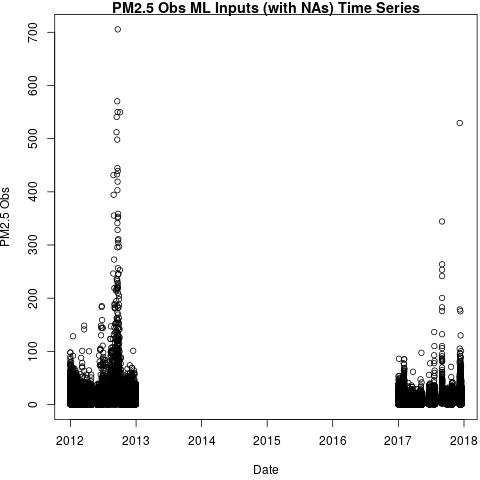
\includegraphics[width=0.77\textwidth]{Code_Outputs/Report_ML_input_PM25_Step4_part_e_de_duplicated_aves_compiled_2019-05-14wNAs_PM25_ObsvDate.jpg} 
\caption{\label{fig:Report_ML_input_PM25_Step4_part_e_de_duplicated_aves_compiled_2019-05-14wNAsPM25_ObsvDate}ML Inputs (with NAs) Time Series} 
\end{figure} 
 

\begin{figure} 
\centering  
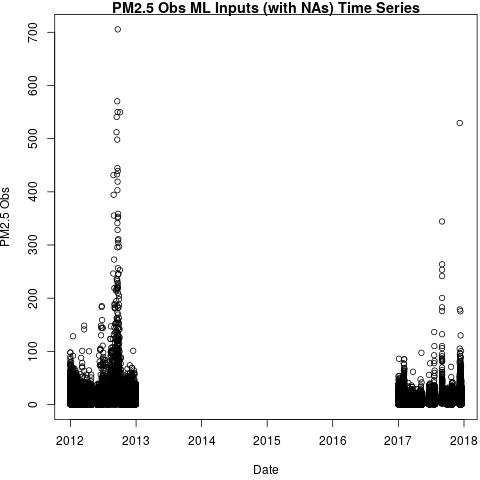
\includegraphics[width=0.77\textwidth]{Code_Outputs/Report_ML_input_PM25_Step4_part_e_de_duplicated_aves_compiled_2019-05-14wNAs_PM25_ObsvDate.jpg} 
\caption{\label{fig:Report_ML_input_PM25_Step4_part_e_de_duplicated_aves_compiled_2019-05-14wNAsPM25_ObsvDate}ML Inputs (with NAs) Time Series} 
\end{figure} 
 

\begin{figure} 
\centering  
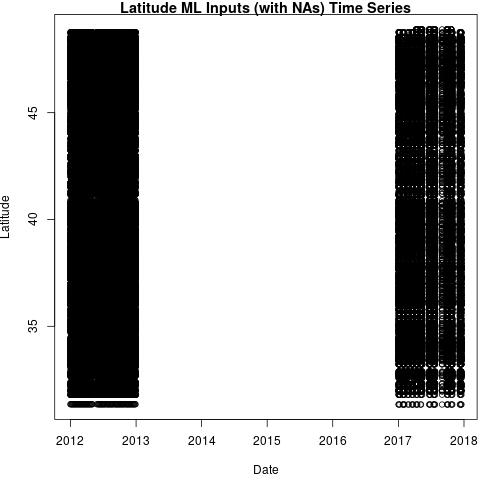
\includegraphics[width=0.77\textwidth]{Code_Outputs/Report_ML_input_PM25_Step4_part_e_de_duplicated_aves_compiled_2019-05-14wNAs_LatitudevDate.jpg} 
\caption{\label{fig:Report_ML_input_PM25_Step4_part_e_de_duplicated_aves_compiled_2019-05-14wNAsLatitudevDate}ML Inputs (with NAs) Time Series} 
\end{figure} 
 

\begin{figure} 
\centering  
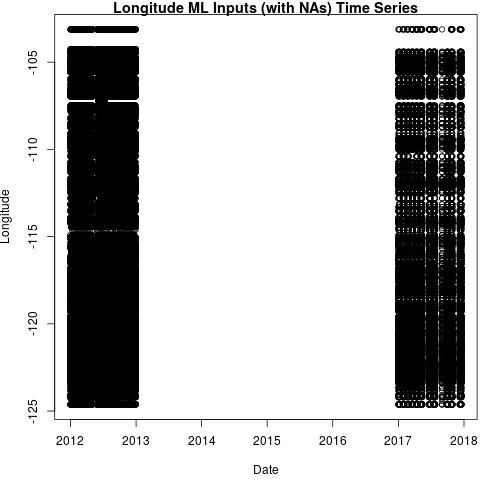
\includegraphics[width=0.77\textwidth]{Code_Outputs/Report_ML_input_PM25_Step4_part_e_de_duplicated_aves_compiled_2019-05-14wNAs_LongitudevDate.jpg} 
\caption{\label{fig:Report_ML_input_PM25_Step4_part_e_de_duplicated_aves_compiled_2019-05-14wNAsLongitudevDate}ML Inputs (with NAs) Time Series} 
\end{figure} 
 

\begin{figure} 
\centering  
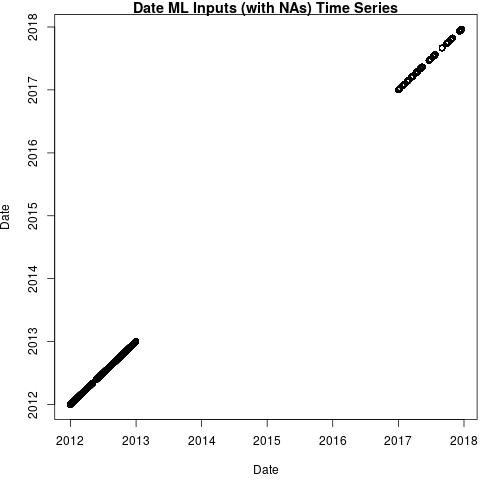
\includegraphics[width=0.77\textwidth]{Code_Outputs/Report_ML_input_PM25_Step4_part_e_de_duplicated_aves_compiled_2019-05-14wNAs_DatevDate.jpg} 
\caption{\label{fig:Report_ML_input_PM25_Step4_part_e_de_duplicated_aves_compiled_2019-05-14wNAsDatevDate}ML Inputs (with NAs) Time Series} 
\end{figure} 
 

\begin{figure} 
\centering  
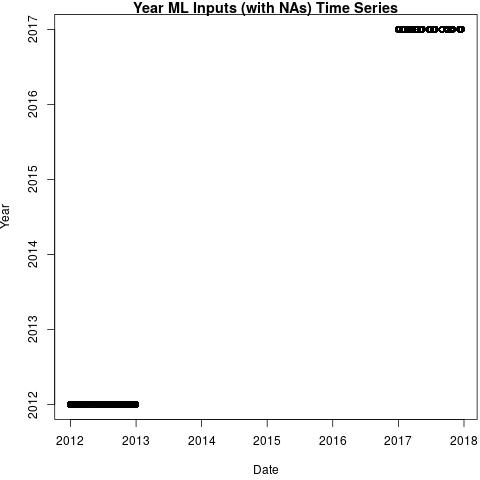
\includegraphics[width=0.77\textwidth]{Code_Outputs/Report_ML_input_PM25_Step4_part_e_de_duplicated_aves_compiled_2019-05-14wNAs_YearvDate.jpg} 
\caption{\label{fig:Report_ML_input_PM25_Step4_part_e_de_duplicated_aves_compiled_2019-05-14wNAsYearvDate}ML Inputs (with NAs) Time Series} 
\end{figure} 
 

\begin{figure} 
\centering  
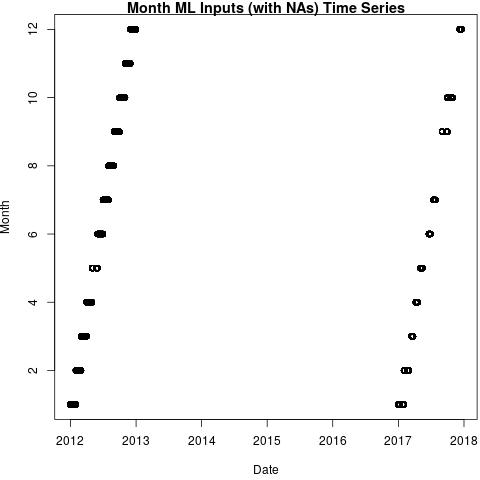
\includegraphics[width=0.77\textwidth]{Code_Outputs/Report_ML_input_PM25_Step4_part_e_de_duplicated_aves_compiled_2019-05-14wNAs_MonthvDate.jpg} 
\caption{\label{fig:Report_ML_input_PM25_Step4_part_e_de_duplicated_aves_compiled_2019-05-14wNAsMonthvDate}ML Inputs (with NAs) Time Series} 
\end{figure} 
 

\begin{figure} 
\centering  
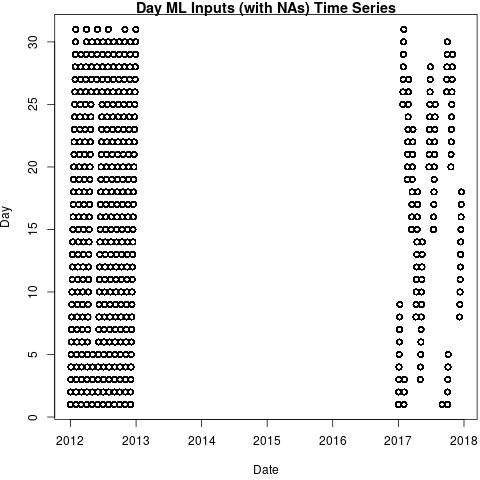
\includegraphics[width=0.77\textwidth]{Code_Outputs/Report_ML_input_PM25_Step4_part_e_de_duplicated_aves_compiled_2019-05-14wNAs_DayvDate.jpg} 
\caption{\label{fig:Report_ML_input_PM25_Step4_part_e_de_duplicated_aves_compiled_2019-05-14wNAsDayvDate}ML Inputs (with NAs) Time Series} 
\end{figure} 
 

\begin{figure} 
\centering  
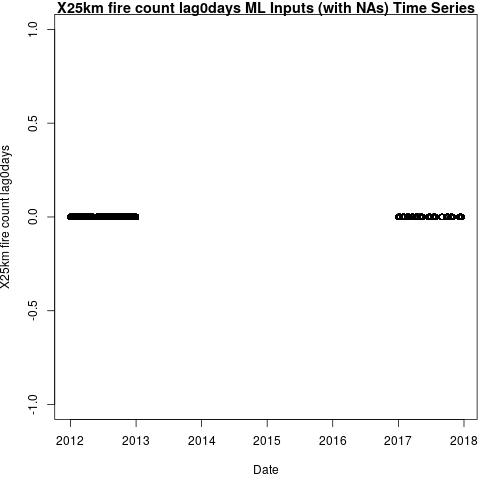
\includegraphics[width=0.77\textwidth]{Code_Outputs/Report_ML_input_PM25_Step4_part_e_de_duplicated_aves_compiled_2019-05-14wNAs_X25km_fire_count_lag0daysvDate.jpg} 
\caption{\label{fig:Report_ML_input_PM25_Step4_part_e_de_duplicated_aves_compiled_2019-05-14wNAsX25km_fire_count_lag0daysvDate}ML Inputs (with NAs) Time Series} 
\end{figure} 
 

\clearpage 

\begin{figure} 
\centering  
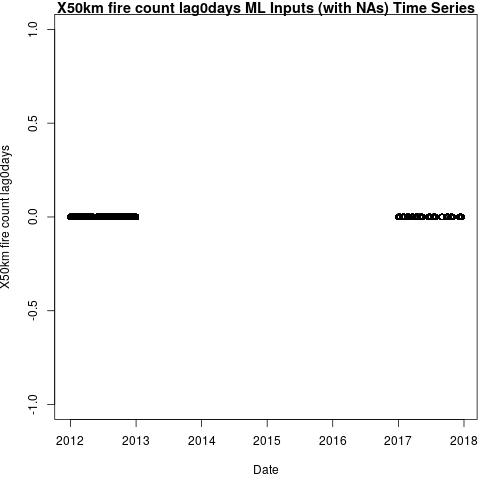
\includegraphics[width=0.77\textwidth]{Code_Outputs/Report_ML_input_PM25_Step4_part_e_de_duplicated_aves_compiled_2019-05-14wNAs_X50km_fire_count_lag0daysvDate.jpg} 
\caption{\label{fig:Report_ML_input_PM25_Step4_part_e_de_duplicated_aves_compiled_2019-05-14wNAsX50km_fire_count_lag0daysvDate}ML Inputs (with NAs) Time Series} 
\end{figure} 
 

\begin{figure} 
\centering  
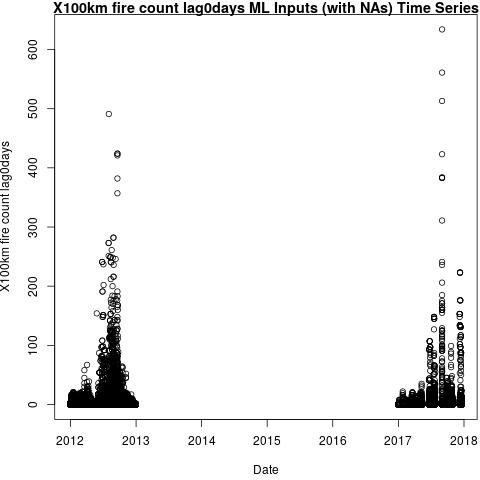
\includegraphics[width=0.77\textwidth]{Code_Outputs/Report_ML_input_PM25_Step4_part_e_de_duplicated_aves_compiled_2019-05-14wNAs_X100km_fire_count_lag0daysvDate.jpg} 
\caption{\label{fig:Report_ML_input_PM25_Step4_part_e_de_duplicated_aves_compiled_2019-05-14wNAsX100km_fire_count_lag0daysvDate}ML Inputs (with NAs) Time Series} 
\end{figure} 
 

\begin{figure} 
\centering  
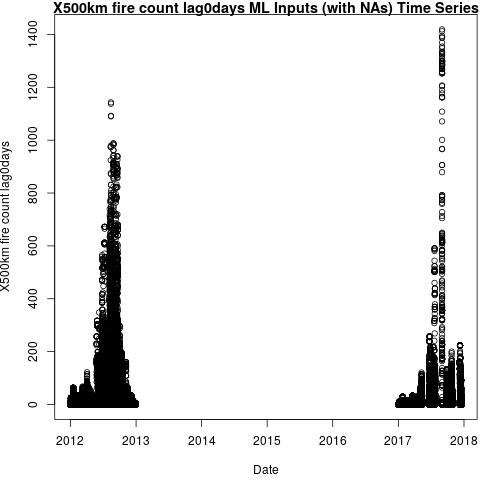
\includegraphics[width=0.77\textwidth]{Code_Outputs/Report_ML_input_PM25_Step4_part_e_de_duplicated_aves_compiled_2019-05-14wNAs_X500km_fire_count_lag0daysvDate.jpg} 
\caption{\label{fig:Report_ML_input_PM25_Step4_part_e_de_duplicated_aves_compiled_2019-05-14wNAsX500km_fire_count_lag0daysvDate}ML Inputs (with NAs) Time Series} 
\end{figure} 
 

\begin{figure} 
\centering  
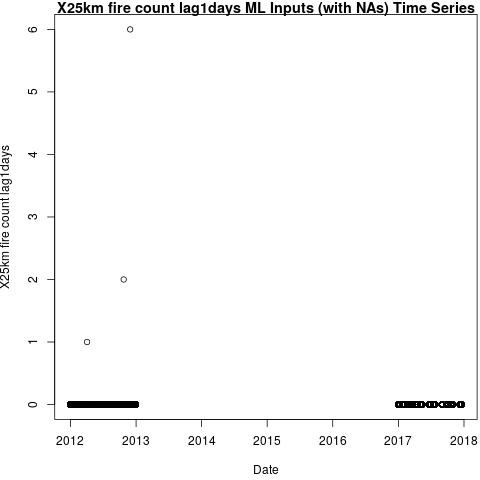
\includegraphics[width=0.77\textwidth]{Code_Outputs/Report_ML_input_PM25_Step4_part_e_de_duplicated_aves_compiled_2019-05-14wNAs_X25km_fire_count_lag1daysvDate.jpg} 
\caption{\label{fig:Report_ML_input_PM25_Step4_part_e_de_duplicated_aves_compiled_2019-05-14wNAsX25km_fire_count_lag1daysvDate}ML Inputs (with NAs) Time Series} 
\end{figure} 
 

\begin{figure} 
\centering  
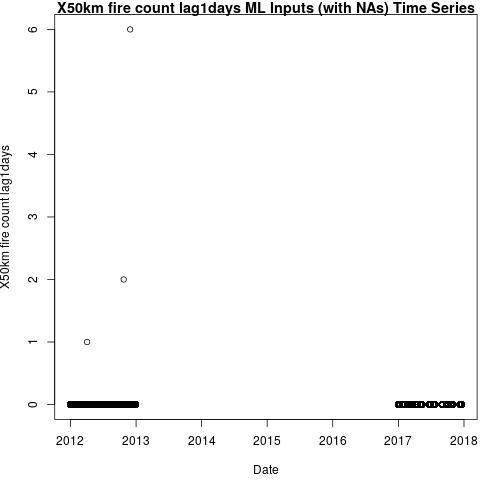
\includegraphics[width=0.77\textwidth]{Code_Outputs/Report_ML_input_PM25_Step4_part_e_de_duplicated_aves_compiled_2019-05-14wNAs_X50km_fire_count_lag1daysvDate.jpg} 
\caption{\label{fig:Report_ML_input_PM25_Step4_part_e_de_duplicated_aves_compiled_2019-05-14wNAsX50km_fire_count_lag1daysvDate}ML Inputs (with NAs) Time Series} 
\end{figure} 
 

\begin{figure} 
\centering  
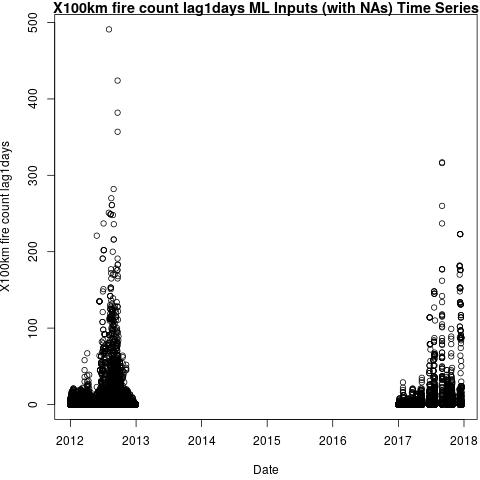
\includegraphics[width=0.77\textwidth]{Code_Outputs/Report_ML_input_PM25_Step4_part_e_de_duplicated_aves_compiled_2019-05-14wNAs_X100km_fire_count_lag1daysvDate.jpg} 
\caption{\label{fig:Report_ML_input_PM25_Step4_part_e_de_duplicated_aves_compiled_2019-05-14wNAsX100km_fire_count_lag1daysvDate}ML Inputs (with NAs) Time Series} 
\end{figure} 
 

\begin{figure} 
\centering  
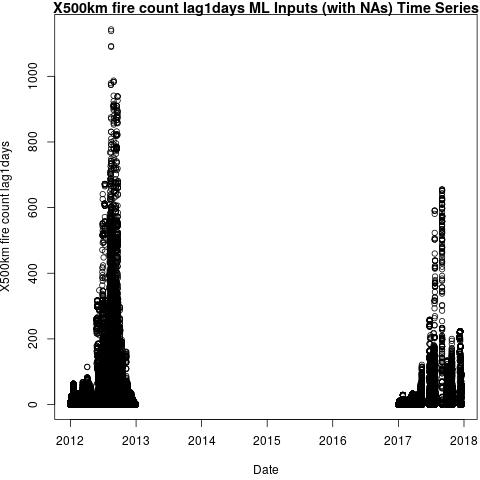
\includegraphics[width=0.77\textwidth]{Code_Outputs/Report_ML_input_PM25_Step4_part_e_de_duplicated_aves_compiled_2019-05-14wNAs_X500km_fire_count_lag1daysvDate.jpg} 
\caption{\label{fig:Report_ML_input_PM25_Step4_part_e_de_duplicated_aves_compiled_2019-05-14wNAsX500km_fire_count_lag1daysvDate}ML Inputs (with NAs) Time Series} 
\end{figure} 
 

\begin{figure} 
\centering  
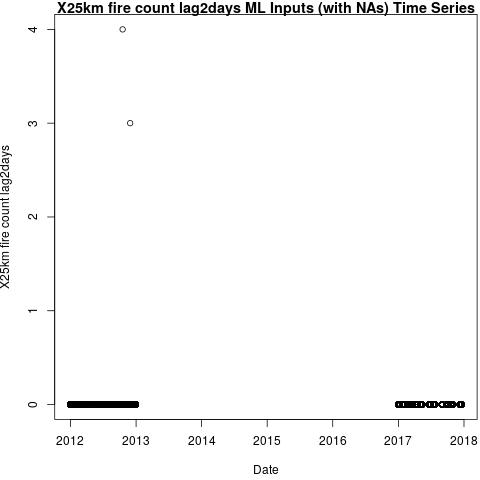
\includegraphics[width=0.77\textwidth]{Code_Outputs/Report_ML_input_PM25_Step4_part_e_de_duplicated_aves_compiled_2019-05-14wNAs_X25km_fire_count_lag2daysvDate.jpg} 
\caption{\label{fig:Report_ML_input_PM25_Step4_part_e_de_duplicated_aves_compiled_2019-05-14wNAsX25km_fire_count_lag2daysvDate}ML Inputs (with NAs) Time Series} 
\end{figure} 
 

\begin{figure} 
\centering  
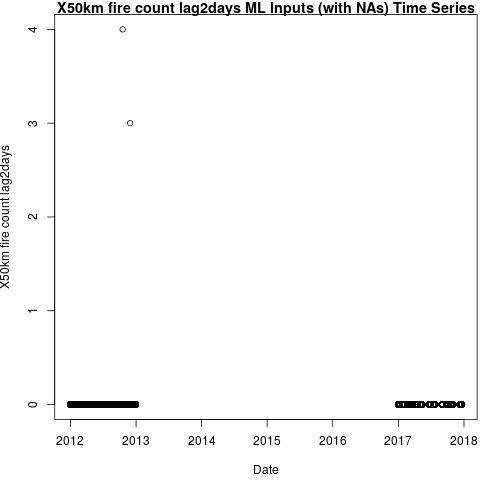
\includegraphics[width=0.77\textwidth]{Code_Outputs/Report_ML_input_PM25_Step4_part_e_de_duplicated_aves_compiled_2019-05-14wNAs_X50km_fire_count_lag2daysvDate.jpg} 
\caption{\label{fig:Report_ML_input_PM25_Step4_part_e_de_duplicated_aves_compiled_2019-05-14wNAsX50km_fire_count_lag2daysvDate}ML Inputs (with NAs) Time Series} 
\end{figure} 
 

\begin{figure} 
\centering  
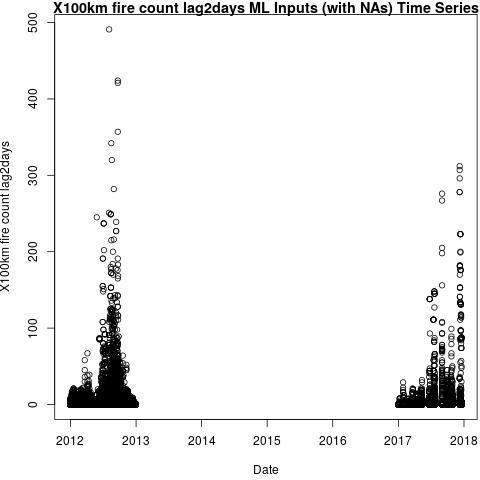
\includegraphics[width=0.77\textwidth]{Code_Outputs/Report_ML_input_PM25_Step4_part_e_de_duplicated_aves_compiled_2019-05-14wNAs_X100km_fire_count_lag2daysvDate.jpg} 
\caption{\label{fig:Report_ML_input_PM25_Step4_part_e_de_duplicated_aves_compiled_2019-05-14wNAsX100km_fire_count_lag2daysvDate}ML Inputs (with NAs) Time Series} 
\end{figure} 
 

\clearpage 

\begin{figure} 
\centering  
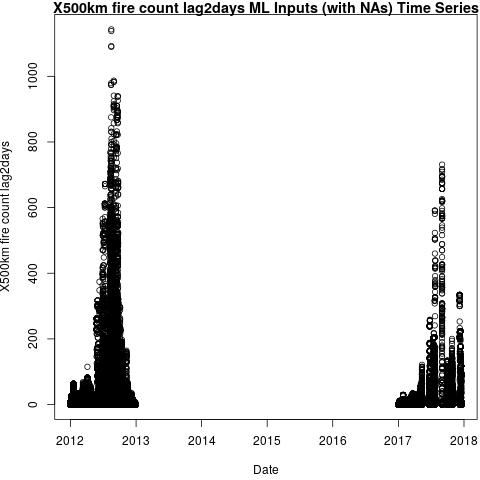
\includegraphics[width=0.77\textwidth]{Code_Outputs/Report_ML_input_PM25_Step4_part_e_de_duplicated_aves_compiled_2019-05-14wNAs_X500km_fire_count_lag2daysvDate.jpg} 
\caption{\label{fig:Report_ML_input_PM25_Step4_part_e_de_duplicated_aves_compiled_2019-05-14wNAsX500km_fire_count_lag2daysvDate}ML Inputs (with NAs) Time Series} 
\end{figure} 
 

\begin{figure} 
\centering  
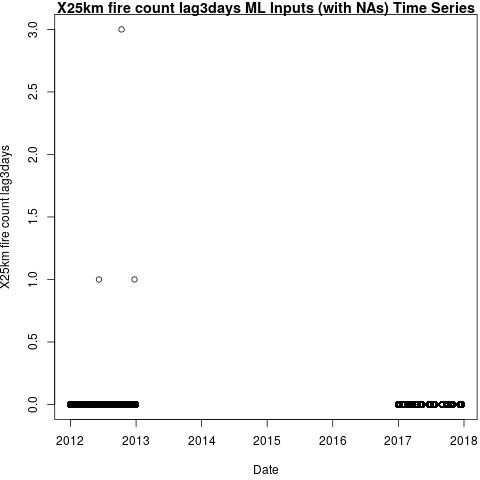
\includegraphics[width=0.77\textwidth]{Code_Outputs/Report_ML_input_PM25_Step4_part_e_de_duplicated_aves_compiled_2019-05-14wNAs_X25km_fire_count_lag3daysvDate.jpg} 
\caption{\label{fig:Report_ML_input_PM25_Step4_part_e_de_duplicated_aves_compiled_2019-05-14wNAsX25km_fire_count_lag3daysvDate}ML Inputs (with NAs) Time Series} 
\end{figure} 
 

\begin{figure} 
\centering  
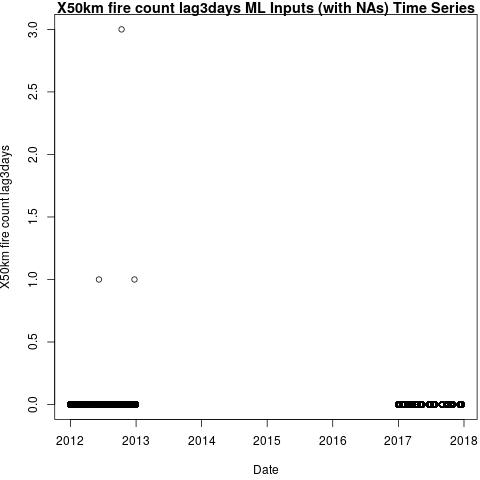
\includegraphics[width=0.77\textwidth]{Code_Outputs/Report_ML_input_PM25_Step4_part_e_de_duplicated_aves_compiled_2019-05-14wNAs_X50km_fire_count_lag3daysvDate.jpg} 
\caption{\label{fig:Report_ML_input_PM25_Step4_part_e_de_duplicated_aves_compiled_2019-05-14wNAsX50km_fire_count_lag3daysvDate}ML Inputs (with NAs) Time Series} 
\end{figure} 
 

\begin{figure} 
\centering  
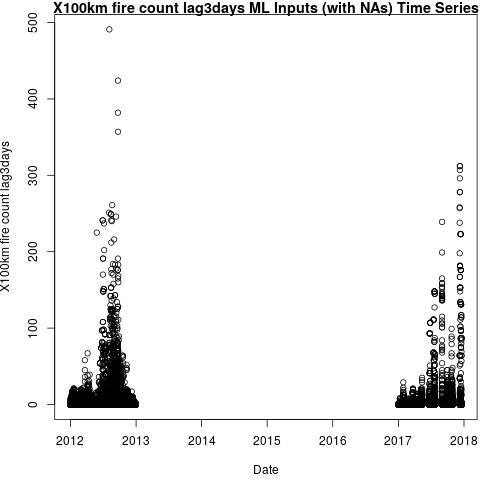
\includegraphics[width=0.77\textwidth]{Code_Outputs/Report_ML_input_PM25_Step4_part_e_de_duplicated_aves_compiled_2019-05-14wNAs_X100km_fire_count_lag3daysvDate.jpg} 
\caption{\label{fig:Report_ML_input_PM25_Step4_part_e_de_duplicated_aves_compiled_2019-05-14wNAsX100km_fire_count_lag3daysvDate}ML Inputs (with NAs) Time Series} 
\end{figure} 
 

\begin{figure} 
\centering  
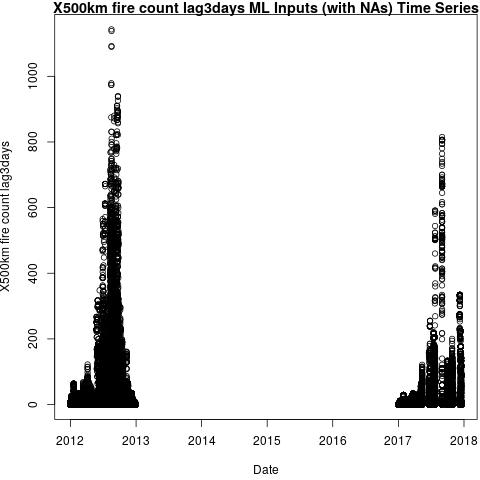
\includegraphics[width=0.77\textwidth]{Code_Outputs/Report_ML_input_PM25_Step4_part_e_de_duplicated_aves_compiled_2019-05-14wNAs_X500km_fire_count_lag3daysvDate.jpg} 
\caption{\label{fig:Report_ML_input_PM25_Step4_part_e_de_duplicated_aves_compiled_2019-05-14wNAsX500km_fire_count_lag3daysvDate}ML Inputs (with NAs) Time Series} 
\end{figure} 
 

\begin{figure} 
\centering  
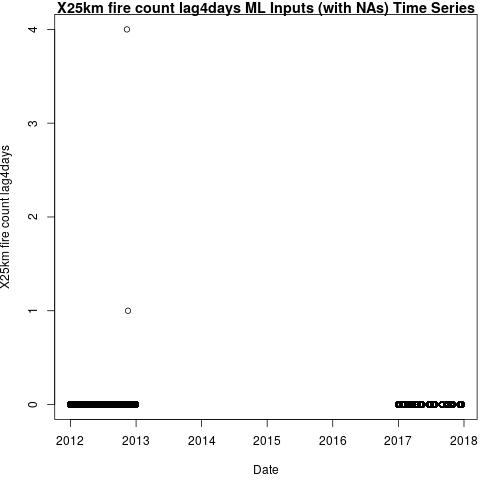
\includegraphics[width=0.77\textwidth]{Code_Outputs/Report_ML_input_PM25_Step4_part_e_de_duplicated_aves_compiled_2019-05-14wNAs_X25km_fire_count_lag4daysvDate.jpg} 
\caption{\label{fig:Report_ML_input_PM25_Step4_part_e_de_duplicated_aves_compiled_2019-05-14wNAsX25km_fire_count_lag4daysvDate}ML Inputs (with NAs) Time Series} 
\end{figure} 
 

\begin{figure} 
\centering  
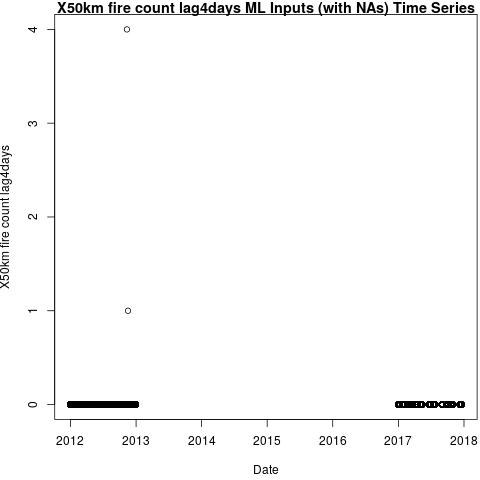
\includegraphics[width=0.77\textwidth]{Code_Outputs/Report_ML_input_PM25_Step4_part_e_de_duplicated_aves_compiled_2019-05-14wNAs_X50km_fire_count_lag4daysvDate.jpg} 
\caption{\label{fig:Report_ML_input_PM25_Step4_part_e_de_duplicated_aves_compiled_2019-05-14wNAsX50km_fire_count_lag4daysvDate}ML Inputs (with NAs) Time Series} 
\end{figure} 
 

\begin{figure} 
\centering  
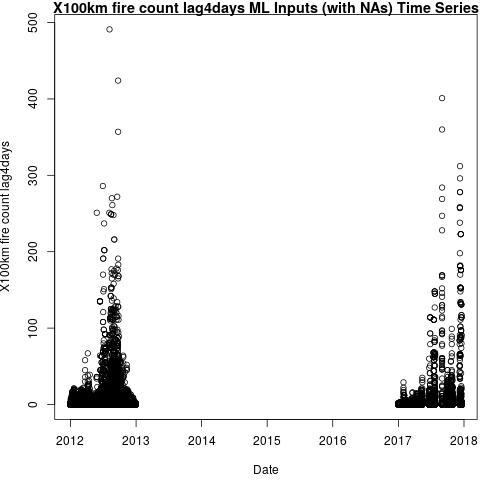
\includegraphics[width=0.77\textwidth]{Code_Outputs/Report_ML_input_PM25_Step4_part_e_de_duplicated_aves_compiled_2019-05-14wNAs_X100km_fire_count_lag4daysvDate.jpg} 
\caption{\label{fig:Report_ML_input_PM25_Step4_part_e_de_duplicated_aves_compiled_2019-05-14wNAsX100km_fire_count_lag4daysvDate}ML Inputs (with NAs) Time Series} 
\end{figure} 
 

\begin{figure} 
\centering  
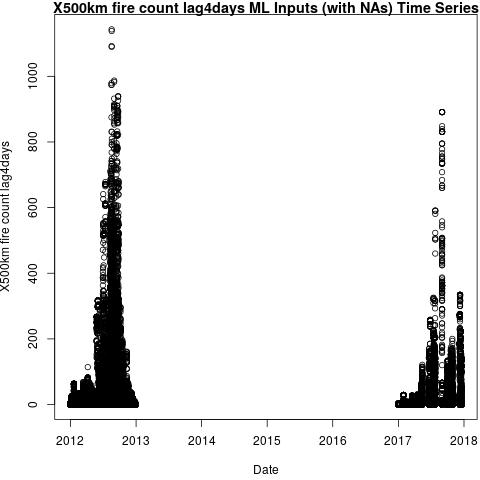
\includegraphics[width=0.77\textwidth]{Code_Outputs/Report_ML_input_PM25_Step4_part_e_de_duplicated_aves_compiled_2019-05-14wNAs_X500km_fire_count_lag4daysvDate.jpg} 
\caption{\label{fig:Report_ML_input_PM25_Step4_part_e_de_duplicated_aves_compiled_2019-05-14wNAsX500km_fire_count_lag4daysvDate}ML Inputs (with NAs) Time Series} 
\end{figure} 
 

\begin{figure} 
\centering  
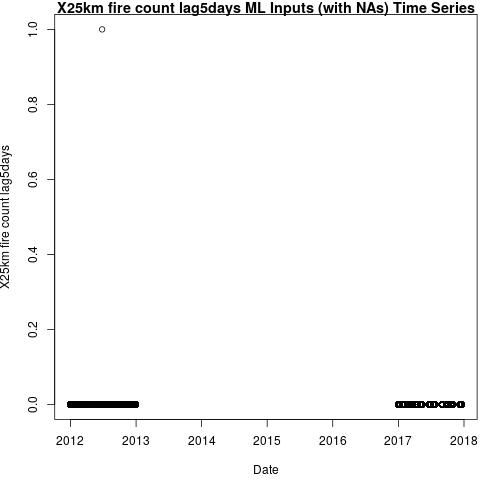
\includegraphics[width=0.77\textwidth]{Code_Outputs/Report_ML_input_PM25_Step4_part_e_de_duplicated_aves_compiled_2019-05-14wNAs_X25km_fire_count_lag5daysvDate.jpg} 
\caption{\label{fig:Report_ML_input_PM25_Step4_part_e_de_duplicated_aves_compiled_2019-05-14wNAsX25km_fire_count_lag5daysvDate}ML Inputs (with NAs) Time Series} 
\end{figure} 
 

\clearpage 

\begin{figure} 
\centering  
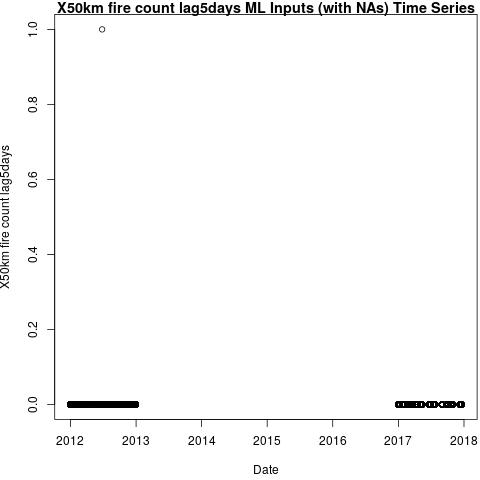
\includegraphics[width=0.77\textwidth]{Code_Outputs/Report_ML_input_PM25_Step4_part_e_de_duplicated_aves_compiled_2019-05-14wNAs_X50km_fire_count_lag5daysvDate.jpg} 
\caption{\label{fig:Report_ML_input_PM25_Step4_part_e_de_duplicated_aves_compiled_2019-05-14wNAsX50km_fire_count_lag5daysvDate}ML Inputs (with NAs) Time Series} 
\end{figure} 
 

\begin{figure} 
\centering  
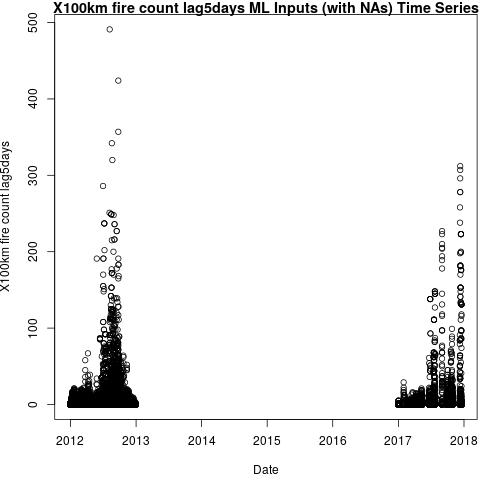
\includegraphics[width=0.77\textwidth]{Code_Outputs/Report_ML_input_PM25_Step4_part_e_de_duplicated_aves_compiled_2019-05-14wNAs_X100km_fire_count_lag5daysvDate.jpg} 
\caption{\label{fig:Report_ML_input_PM25_Step4_part_e_de_duplicated_aves_compiled_2019-05-14wNAsX100km_fire_count_lag5daysvDate}ML Inputs (with NAs) Time Series} 
\end{figure} 
 

\begin{figure} 
\centering  
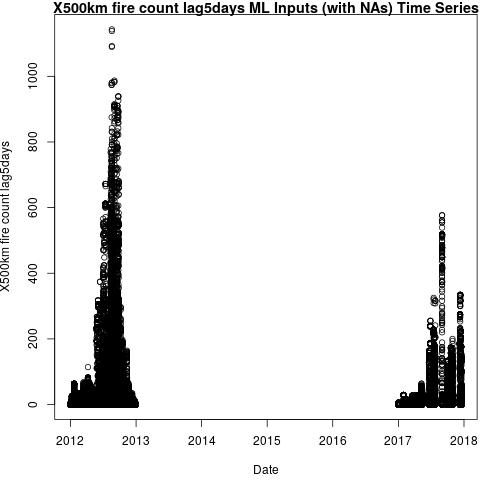
\includegraphics[width=0.77\textwidth]{Code_Outputs/Report_ML_input_PM25_Step4_part_e_de_duplicated_aves_compiled_2019-05-14wNAs_X500km_fire_count_lag5daysvDate.jpg} 
\caption{\label{fig:Report_ML_input_PM25_Step4_part_e_de_duplicated_aves_compiled_2019-05-14wNAsX500km_fire_count_lag5daysvDate}ML Inputs (with NAs) Time Series} 
\end{figure} 
 

\begin{figure} 
\centering  
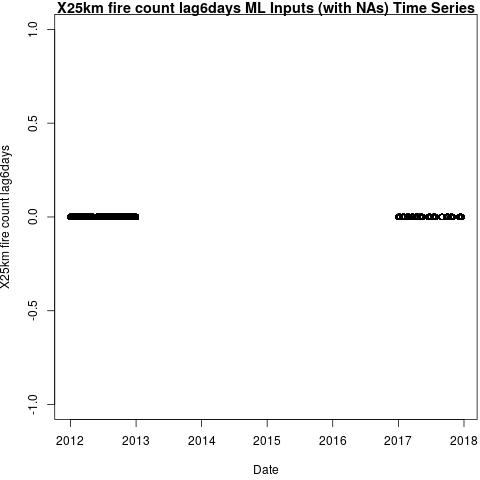
\includegraphics[width=0.77\textwidth]{Code_Outputs/Report_ML_input_PM25_Step4_part_e_de_duplicated_aves_compiled_2019-05-14wNAs_X25km_fire_count_lag6daysvDate.jpg} 
\caption{\label{fig:Report_ML_input_PM25_Step4_part_e_de_duplicated_aves_compiled_2019-05-14wNAsX25km_fire_count_lag6daysvDate}ML Inputs (with NAs) Time Series} 
\end{figure} 
 

\begin{figure} 
\centering  
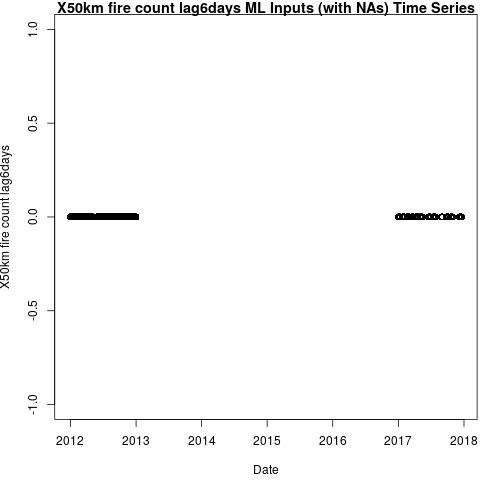
\includegraphics[width=0.77\textwidth]{Code_Outputs/Report_ML_input_PM25_Step4_part_e_de_duplicated_aves_compiled_2019-05-14wNAs_X50km_fire_count_lag6daysvDate.jpg} 
\caption{\label{fig:Report_ML_input_PM25_Step4_part_e_de_duplicated_aves_compiled_2019-05-14wNAsX50km_fire_count_lag6daysvDate}ML Inputs (with NAs) Time Series} 
\end{figure} 
 

\begin{figure} 
\centering  
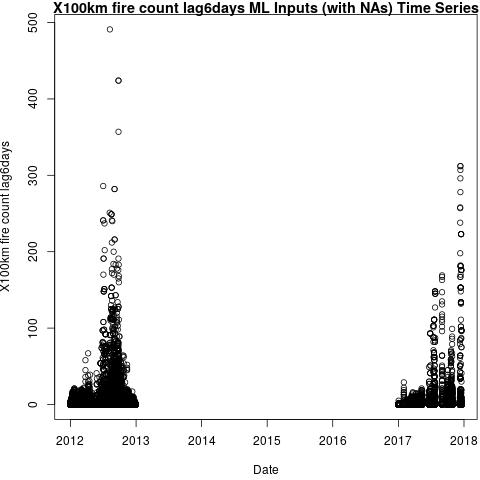
\includegraphics[width=0.77\textwidth]{Code_Outputs/Report_ML_input_PM25_Step4_part_e_de_duplicated_aves_compiled_2019-05-14wNAs_X100km_fire_count_lag6daysvDate.jpg} 
\caption{\label{fig:Report_ML_input_PM25_Step4_part_e_de_duplicated_aves_compiled_2019-05-14wNAsX100km_fire_count_lag6daysvDate}ML Inputs (with NAs) Time Series} 
\end{figure} 
 

\begin{figure} 
\centering  
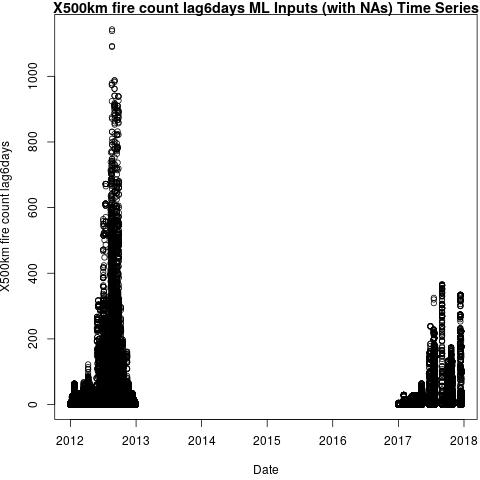
\includegraphics[width=0.77\textwidth]{Code_Outputs/Report_ML_input_PM25_Step4_part_e_de_duplicated_aves_compiled_2019-05-14wNAs_X500km_fire_count_lag6daysvDate.jpg} 
\caption{\label{fig:Report_ML_input_PM25_Step4_part_e_de_duplicated_aves_compiled_2019-05-14wNAsX500km_fire_count_lag6daysvDate}ML Inputs (with NAs) Time Series} 
\end{figure} 
 

\begin{figure} 
\centering  
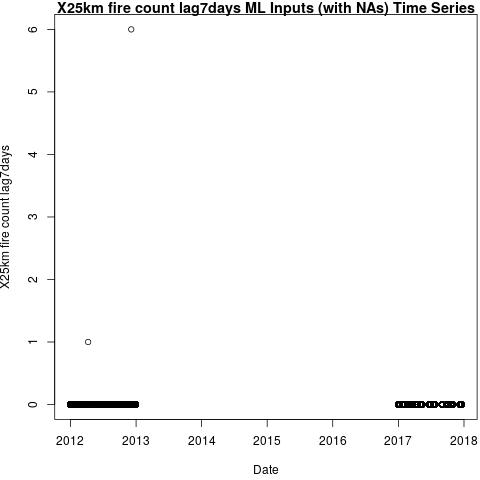
\includegraphics[width=0.77\textwidth]{Code_Outputs/Report_ML_input_PM25_Step4_part_e_de_duplicated_aves_compiled_2019-05-14wNAs_X25km_fire_count_lag7daysvDate.jpg} 
\caption{\label{fig:Report_ML_input_PM25_Step4_part_e_de_duplicated_aves_compiled_2019-05-14wNAsX25km_fire_count_lag7daysvDate}ML Inputs (with NAs) Time Series} 
\end{figure} 
 

\begin{figure} 
\centering  
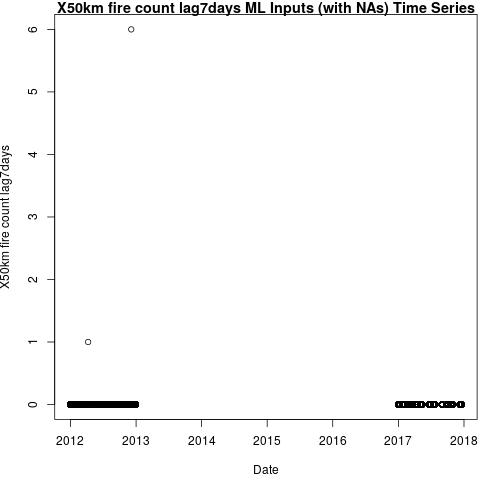
\includegraphics[width=0.77\textwidth]{Code_Outputs/Report_ML_input_PM25_Step4_part_e_de_duplicated_aves_compiled_2019-05-14wNAs_X50km_fire_count_lag7daysvDate.jpg} 
\caption{\label{fig:Report_ML_input_PM25_Step4_part_e_de_duplicated_aves_compiled_2019-05-14wNAsX50km_fire_count_lag7daysvDate}ML Inputs (with NAs) Time Series} 
\end{figure} 
 

\begin{figure} 
\centering  
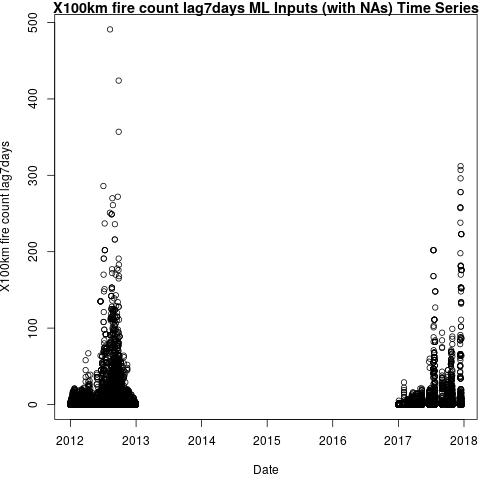
\includegraphics[width=0.77\textwidth]{Code_Outputs/Report_ML_input_PM25_Step4_part_e_de_duplicated_aves_compiled_2019-05-14wNAs_X100km_fire_count_lag7daysvDate.jpg} 
\caption{\label{fig:Report_ML_input_PM25_Step4_part_e_de_duplicated_aves_compiled_2019-05-14wNAsX100km_fire_count_lag7daysvDate}ML Inputs (with NAs) Time Series} 
\end{figure} 
 

\clearpage 

\begin{figure} 
\centering  
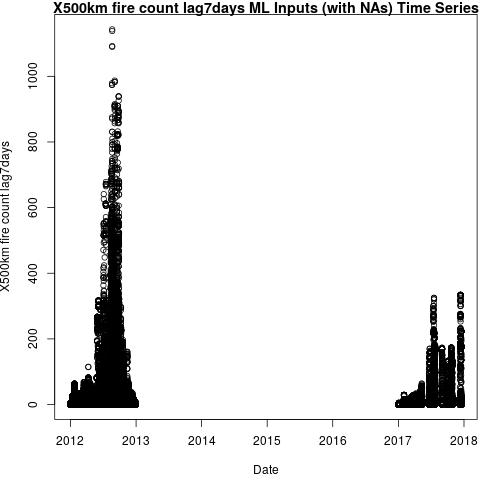
\includegraphics[width=0.77\textwidth]{Code_Outputs/Report_ML_input_PM25_Step4_part_e_de_duplicated_aves_compiled_2019-05-14wNAs_X500km_fire_count_lag7daysvDate.jpg} 
\caption{\label{fig:Report_ML_input_PM25_Step4_part_e_de_duplicated_aves_compiled_2019-05-14wNAsX500km_fire_count_lag7daysvDate}ML Inputs (with NAs) Time Series} 
\end{figure} 
 

\begin{figure} 
\centering  
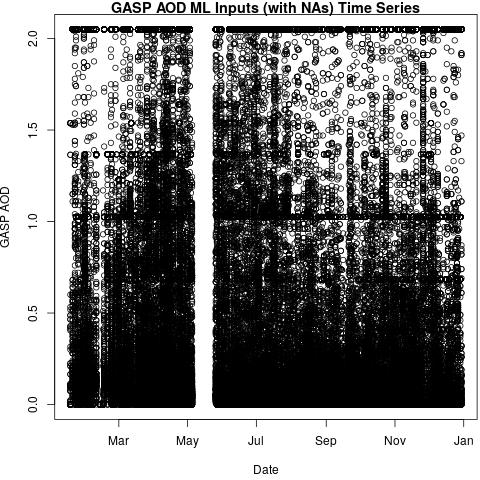
\includegraphics[width=0.77\textwidth]{Code_Outputs/Report_ML_input_PM25_Step4_part_e_de_duplicated_aves_compiled_2019-05-14wNAs_GASP_AODvDate.jpg} 
\caption{\label{fig:Report_ML_input_PM25_Step4_part_e_de_duplicated_aves_compiled_2019-05-14wNAsGASP_AODvDate}ML Inputs (with NAs) Time Series} 
\end{figure} 
 

\begin{figure} 
\centering  
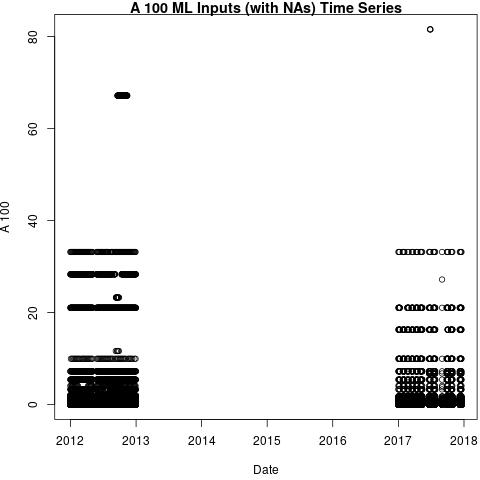
\includegraphics[width=0.77\textwidth]{Code_Outputs/Report_ML_input_PM25_Step4_part_e_de_duplicated_aves_compiled_2019-05-14wNAs_A_100vDate.jpg} 
\caption{\label{fig:Report_ML_input_PM25_Step4_part_e_de_duplicated_aves_compiled_2019-05-14wNAsA_100vDate}ML Inputs (with NAs) Time Series} 
\end{figure} 
 

\begin{figure} 
\centering  
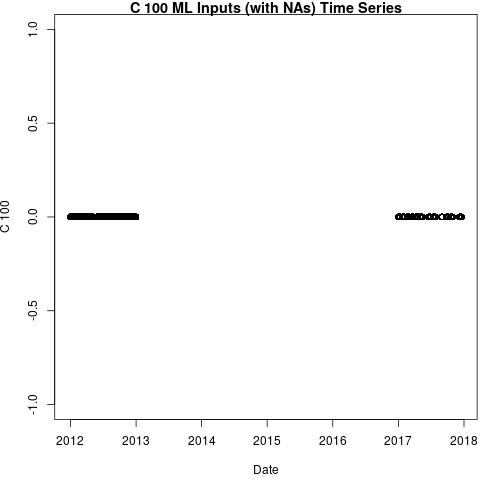
\includegraphics[width=0.77\textwidth]{Code_Outputs/Report_ML_input_PM25_Step4_part_e_de_duplicated_aves_compiled_2019-05-14wNAs_C_100vDate.jpg} 
\caption{\label{fig:Report_ML_input_PM25_Step4_part_e_de_duplicated_aves_compiled_2019-05-14wNAsC_100vDate}ML Inputs (with NAs) Time Series} 
\end{figure} 
 

\begin{figure} 
\centering  
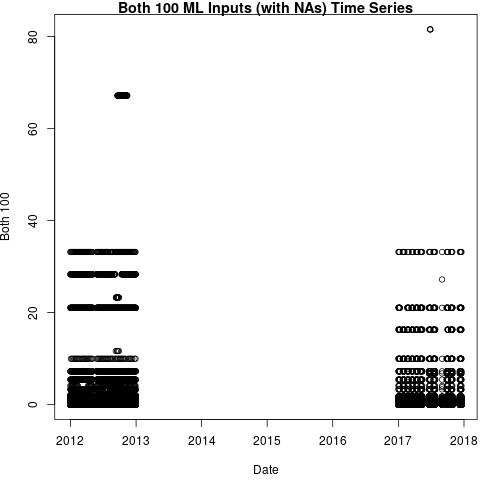
\includegraphics[width=0.77\textwidth]{Code_Outputs/Report_ML_input_PM25_Step4_part_e_de_duplicated_aves_compiled_2019-05-14wNAs_Both_100vDate.jpg} 
\caption{\label{fig:Report_ML_input_PM25_Step4_part_e_de_duplicated_aves_compiled_2019-05-14wNAsBoth_100vDate}ML Inputs (with NAs) Time Series} 
\end{figure} 
 

\begin{figure} 
\centering  
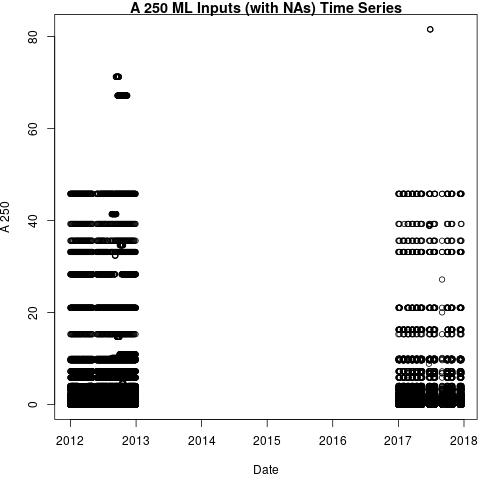
\includegraphics[width=0.77\textwidth]{Code_Outputs/Report_ML_input_PM25_Step4_part_e_de_duplicated_aves_compiled_2019-05-14wNAs_A_250vDate.jpg} 
\caption{\label{fig:Report_ML_input_PM25_Step4_part_e_de_duplicated_aves_compiled_2019-05-14wNAsA_250vDate}ML Inputs (with NAs) Time Series} 
\end{figure} 
 

\begin{figure} 
\centering  
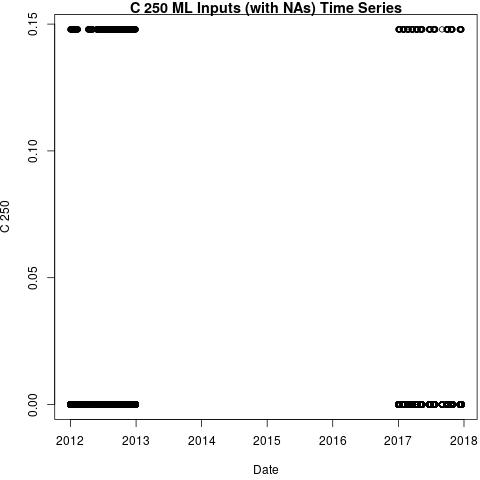
\includegraphics[width=0.77\textwidth]{Code_Outputs/Report_ML_input_PM25_Step4_part_e_de_duplicated_aves_compiled_2019-05-14wNAs_C_250vDate.jpg} 
\caption{\label{fig:Report_ML_input_PM25_Step4_part_e_de_duplicated_aves_compiled_2019-05-14wNAsC_250vDate}ML Inputs (with NAs) Time Series} 
\end{figure} 
 

\begin{figure} 
\centering  
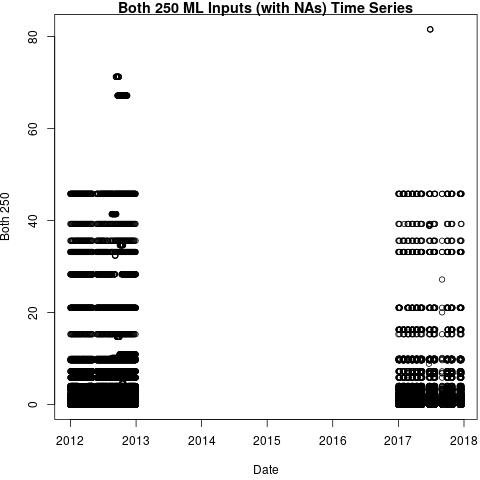
\includegraphics[width=0.77\textwidth]{Code_Outputs/Report_ML_input_PM25_Step4_part_e_de_duplicated_aves_compiled_2019-05-14wNAs_Both_250vDate.jpg} 
\caption{\label{fig:Report_ML_input_PM25_Step4_part_e_de_duplicated_aves_compiled_2019-05-14wNAsBoth_250vDate}ML Inputs (with NAs) Time Series} 
\end{figure} 
 

\begin{figure} 
\centering  
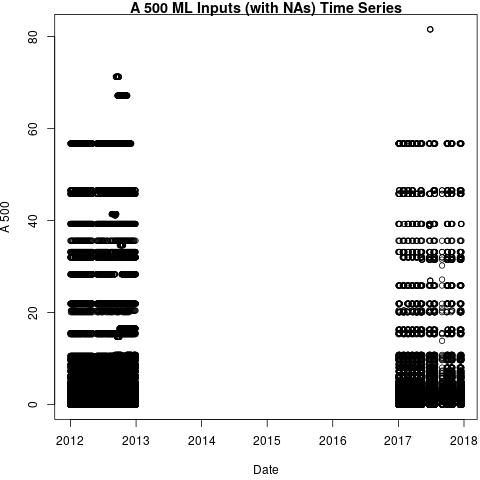
\includegraphics[width=0.77\textwidth]{Code_Outputs/Report_ML_input_PM25_Step4_part_e_de_duplicated_aves_compiled_2019-05-14wNAs_A_500vDate.jpg} 
\caption{\label{fig:Report_ML_input_PM25_Step4_part_e_de_duplicated_aves_compiled_2019-05-14wNAsA_500vDate}ML Inputs (with NAs) Time Series} 
\end{figure} 
 

\begin{figure} 
\centering  
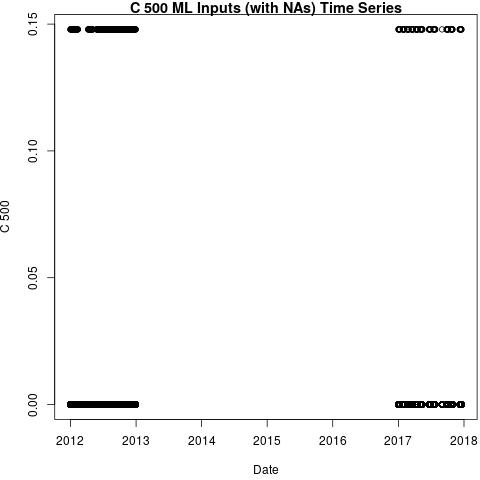
\includegraphics[width=0.77\textwidth]{Code_Outputs/Report_ML_input_PM25_Step4_part_e_de_duplicated_aves_compiled_2019-05-14wNAs_C_500vDate.jpg} 
\caption{\label{fig:Report_ML_input_PM25_Step4_part_e_de_duplicated_aves_compiled_2019-05-14wNAsC_500vDate}ML Inputs (with NAs) Time Series} 
\end{figure} 
 

\clearpage 

\begin{figure} 
\centering  
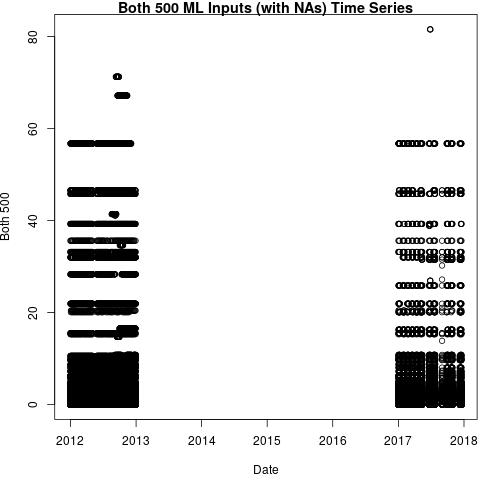
\includegraphics[width=0.77\textwidth]{Code_Outputs/Report_ML_input_PM25_Step4_part_e_de_duplicated_aves_compiled_2019-05-14wNAs_Both_500vDate.jpg} 
\caption{\label{fig:Report_ML_input_PM25_Step4_part_e_de_duplicated_aves_compiled_2019-05-14wNAsBoth_500vDate}ML Inputs (with NAs) Time Series} 
\end{figure} 
 

\begin{figure} 
\centering  
\includegraphics[width=0.77\textwidth]{Code_Outputs/Report_ML_input_PM25_Step4_part_e_de_duplicated_aves_compiled_2019-05-14wNAs_A_1000vDate.jpg} 
\caption{\label{fig:Report_ML_input_PM25_Step4_part_e_de_duplicated_aves_compiled_2019-05-14wNAsA_1000vDate}ML Inputs (with NAs) Time Series} 
\end{figure} 
 

\begin{figure} 
\centering  
\includegraphics[width=0.77\textwidth]{Code_Outputs/Report_ML_input_PM25_Step4_part_e_de_duplicated_aves_compiled_2019-05-14wNAs_C_1000vDate.jpg} 
\caption{\label{fig:Report_ML_input_PM25_Step4_part_e_de_duplicated_aves_compiled_2019-05-14wNAsC_1000vDate}ML Inputs (with NAs) Time Series} 
\end{figure} 
 

\begin{figure} 
\centering  
\includegraphics[width=0.77\textwidth]{Code_Outputs/Report_ML_input_PM25_Step4_part_e_de_duplicated_aves_compiled_2019-05-14wNAs_Both_1000vDate.jpg} 
\caption{\label{fig:Report_ML_input_PM25_Step4_part_e_de_duplicated_aves_compiled_2019-05-14wNAsBoth_1000vDate}ML Inputs (with NAs) Time Series} 
\end{figure} 
 

\begin{figure} 
\centering  
\includegraphics[width=0.77\textwidth]{Code_Outputs/Report_ML_input_PM25_Step4_part_e_de_duplicated_aves_compiled_2019-05-14wNAs_MAIAC_AODvDate.jpg} 
\caption{\label{fig:Report_ML_input_PM25_Step4_part_e_de_duplicated_aves_compiled_2019-05-14wNAsMAIAC_AODvDate}ML Inputs (with NAs) Time Series} 
\end{figure} 
 

\begin{figure} 
\centering  
\includegraphics[width=0.77\textwidth]{Code_Outputs/Report_ML_input_PM25_Step4_part_e_de_duplicated_aves_compiled_2019-05-14wNAs_elevationvDate.jpg} 
\caption{\label{fig:Report_ML_input_PM25_Step4_part_e_de_duplicated_aves_compiled_2019-05-14wNAselevationvDate}ML Inputs (with NAs) Time Series} 
\end{figure} 
 

\begin{figure} 
\centering  
\includegraphics[width=0.77\textwidth]{Code_Outputs/Report_ML_input_PM25_Step4_part_e_de_duplicated_aves_compiled_2019-05-14wNAs_HPBLsurfacevDate.jpg} 
\caption{\label{fig:Report_ML_input_PM25_Step4_part_e_de_duplicated_aves_compiled_2019-05-14wNAsHPBLsurfacevDate}ML Inputs (with NAs) Time Series} 
\end{figure} 
 

\begin{figure} 
\centering  
\includegraphics[width=0.77\textwidth]{Code_Outputs/Report_ML_input_PM25_Step4_part_e_de_duplicated_aves_compiled_2019-05-14wNAs_TMP2mabovegroundvDate.jpg} 
\caption{\label{fig:Report_ML_input_PM25_Step4_part_e_de_duplicated_aves_compiled_2019-05-14wNAsTMP2mabovegroundvDate}ML Inputs (with NAs) Time Series} 
\end{figure} 
 

\begin{figure} 
\centering  
\includegraphics[width=0.77\textwidth]{Code_Outputs/Report_ML_input_PM25_Step4_part_e_de_duplicated_aves_compiled_2019-05-14wNAs_RH2mabovegroundvDate.jpg} 
\caption{\label{fig:Report_ML_input_PM25_Step4_part_e_de_duplicated_aves_compiled_2019-05-14wNAsRH2mabovegroundvDate}ML Inputs (with NAs) Time Series} 
\end{figure} 
 

\begin{figure} 
\centering  
\includegraphics[width=0.77\textwidth]{Code_Outputs/Report_ML_input_PM25_Step4_part_e_de_duplicated_aves_compiled_2019-05-14wNAs_DPT2mabovegroundvDate.jpg} 
\caption{\label{fig:Report_ML_input_PM25_Step4_part_e_de_duplicated_aves_compiled_2019-05-14wNAsDPT2mabovegroundvDate}ML Inputs (with NAs) Time Series} 
\end{figure} 
 

\clearpage 

\begin{figure} 
\centering  
\includegraphics[width=0.77\textwidth]{Code_Outputs/Report_ML_input_PM25_Step4_part_e_de_duplicated_aves_compiled_2019-05-14wNAs_APCPsurfacevDate.jpg} 
\caption{\label{fig:Report_ML_input_PM25_Step4_part_e_de_duplicated_aves_compiled_2019-05-14wNAsAPCPsurfacevDate}ML Inputs (with NAs) Time Series} 
\end{figure} 
 

\begin{figure} 
\centering  
\includegraphics[width=0.77\textwidth]{Code_Outputs/Report_ML_input_PM25_Step4_part_e_de_duplicated_aves_compiled_2019-05-14wNAs_WEASDsurfacevDate.jpg} 
\caption{\label{fig:Report_ML_input_PM25_Step4_part_e_de_duplicated_aves_compiled_2019-05-14wNAsWEASDsurfacevDate}ML Inputs (with NAs) Time Series} 
\end{figure} 
 

\begin{figure} 
\centering  
\includegraphics[width=0.77\textwidth]{Code_Outputs/Report_ML_input_PM25_Step4_part_e_de_duplicated_aves_compiled_2019-05-14wNAs_SNOWCsurfacevDate.jpg} 
\caption{\label{fig:Report_ML_input_PM25_Step4_part_e_de_duplicated_aves_compiled_2019-05-14wNAsSNOWCsurfacevDate}ML Inputs (with NAs) Time Series} 
\end{figure} 
 

\begin{figure} 
\centering  
\includegraphics[width=0.77\textwidth]{Code_Outputs/Report_ML_input_PM25_Step4_part_e_de_duplicated_aves_compiled_2019-05-14wNAs_UGRD10mabovegroundvDate.jpg} 
\caption{\label{fig:Report_ML_input_PM25_Step4_part_e_de_duplicated_aves_compiled_2019-05-14wNAsUGRD10mabovegroundvDate}ML Inputs (with NAs) Time Series} 
\end{figure} 
 

\begin{figure} 
\centering  
\includegraphics[width=0.77\textwidth]{Code_Outputs/Report_ML_input_PM25_Step4_part_e_de_duplicated_aves_compiled_2019-05-14wNAs_VGRD10mabovegroundvDate.jpg} 
\caption{\label{fig:Report_ML_input_PM25_Step4_part_e_de_duplicated_aves_compiled_2019-05-14wNAsVGRD10mabovegroundvDate}ML Inputs (with NAs) Time Series} 
\end{figure} 
 

\begin{figure} 
\centering  
\includegraphics[width=0.77\textwidth]{Code_Outputs/Report_ML_input_PM25_Step4_part_e_de_duplicated_aves_compiled_2019-05-14wNAs_PRMSLmeansealevelvDate.jpg} 
\caption{\label{fig:Report_ML_input_PM25_Step4_part_e_de_duplicated_aves_compiled_2019-05-14wNAsPRMSLmeansealevelvDate}ML Inputs (with NAs) Time Series} 
\end{figure} 
 

\begin{figure} 
\centering  
\includegraphics[width=0.77\textwidth]{Code_Outputs/Report_ML_input_PM25_Step4_part_e_de_duplicated_aves_compiled_2019-05-14wNAs_PRESsurfacevDate.jpg} 
\caption{\label{fig:Report_ML_input_PM25_Step4_part_e_de_duplicated_aves_compiled_2019-05-14wNAsPRESsurfacevDate}ML Inputs (with NAs) Time Series} 
\end{figure} 
 

\begin{figure} 
\centering  
\includegraphics[width=0.77\textwidth]{Code_Outputs/Report_ML_input_PM25_Step4_part_e_de_duplicated_aves_compiled_2019-05-14wNAs_DZDT850mbvDate.jpg} 
\caption{\label{fig:Report_ML_input_PM25_Step4_part_e_de_duplicated_aves_compiled_2019-05-14wNAsDZDT850mbvDate}ML Inputs (with NAs) Time Series} 
\end{figure} 
 

\begin{figure} 
\centering  
\includegraphics[width=0.77\textwidth]{Code_Outputs/Report_ML_input_PM25_Step4_part_e_de_duplicated_aves_compiled_2019-05-14wNAs_DZDT700mbvDate.jpg} 
\caption{\label{fig:Report_ML_input_PM25_Step4_part_e_de_duplicated_aves_compiled_2019-05-14wNAsDZDT700mbvDate}ML Inputs (with NAs) Time Series} 
\end{figure} 
 

\begin{figure} 
\centering  
\includegraphics[width=0.77\textwidth]{Code_Outputs/Report_ML_input_PM25_Step4_part_e_de_duplicated_aves_compiled_2019-05-14wNAs_NLCD_1km_percent_urban_buffervDate.jpg} 
\caption{\label{fig:Report_ML_input_PM25_Step4_part_e_de_duplicated_aves_compiled_2019-05-14wNAsNLCD_1km_percent_urban_buffervDate}ML Inputs (with NAs) Time Series} 
\end{figure} 
 

\clearpage 

\begin{figure} 
\centering  
\includegraphics[width=0.77\textwidth]{Code_Outputs/Report_ML_input_PM25_Step4_part_e_de_duplicated_aves_compiled_2019-05-14wNAs_NLCD_5km_percent_urban_buffervDate.jpg} 
\caption{\label{fig:Report_ML_input_PM25_Step4_part_e_de_duplicated_aves_compiled_2019-05-14wNAsNLCD_5km_percent_urban_buffervDate}ML Inputs (with NAs) Time Series} 
\end{figure} 
 

\begin{figure} 
\centering  
\includegraphics[width=0.77\textwidth]{Code_Outputs/Report_ML_input_PM25_Step4_part_e_de_duplicated_aves_compiled_2019-05-14wNAs_NLCD_10km_percent_urban_buffervDate.jpg} 
\caption{\label{fig:Report_ML_input_PM25_Step4_part_e_de_duplicated_aves_compiled_2019-05-14wNAsNLCD_10km_percent_urban_buffervDate}ML Inputs (with NAs) Time Series} 
\end{figure} 
 

\begin{figure} 
\centering  
\includegraphics[width=0.77\textwidth]{Code_Outputs/Report_ML_input_PM25_Step4_part_e_de_duplicated_aves_compiled_2019-05-14wNAs_DayOfWeekvDate.jpg} 
\caption{\label{fig:Report_ML_input_PM25_Step4_part_e_de_duplicated_aves_compiled_2019-05-14wNAsDayOfWeekvDate}ML Inputs (with NAs) Time Series} 
\end{figure} 
 

\begin{figure} 
\centering  
\includegraphics[width=0.77\textwidth]{Code_Outputs/Report_ML_input_PM25_Step4_part_e_de_duplicated_aves_compiled_2019-05-14wNAs_DecimalDatewYearvDate.jpg} 
\caption{\label{fig:Report_ML_input_PM25_Step4_part_e_de_duplicated_aves_compiled_2019-05-14wNAsDecimalDatewYearvDate}ML Inputs (with NAs) Time Series} 
\end{figure} 
 

\begin{figure} 
\centering  
\includegraphics[width=0.77\textwidth]{Code_Outputs/Report_ML_input_PM25_Step4_part_e_de_duplicated_aves_compiled_2019-05-14wNAs_DecimalDatevDate.jpg} 
\caption{\label{fig:Report_ML_input_PM25_Step4_part_e_de_duplicated_aves_compiled_2019-05-14wNAsDecimalDatevDate}ML Inputs (with NAs) Time Series} 
\end{figure} 
 
 

% PM2.5 vs predictor for each predictor variable 

\subsection{ML Inputs (with NAs) Plot against PM2.5 Obs Images} 
 

\begin{figure} 
\centering  
\includegraphics[width=0.77\textwidth]{Code_Outputs/Report_ML_input_PM25_Step4_part_e_de_duplicated_aves_compiled_2019-05-14wNAs_PM25_ObsvPM25_Obs.jpg} 
\caption{\label{fig:Report_ML_input_PM25_Step4_part_e_de_duplicated_aves_compiled_2019-05-14wNAsPM25_ObsvPM25_Obs}ML Inputs (with NAs) Plot against PM2.5 Obs} 
\end{figure} 
 

\begin{figure} 
\centering  
\includegraphics[width=0.77\textwidth]{Code_Outputs/Report_ML_input_PM25_Step4_part_e_de_duplicated_aves_compiled_2019-05-14wNAs_X25km_fire_count_lag0daysvPM25_Obs.jpg} 
\caption{\label{fig:Report_ML_input_PM25_Step4_part_e_de_duplicated_aves_compiled_2019-05-14wNAsX25km_fire_count_lag0daysvPM25_Obs}ML Inputs (with NAs) Plot against PM2.5 Obs} 
\end{figure} 
 

\begin{figure} 
\centering  
\includegraphics[width=0.77\textwidth]{Code_Outputs/Report_ML_input_PM25_Step4_part_e_de_duplicated_aves_compiled_2019-05-14wNAs_X50km_fire_count_lag0daysvPM25_Obs.jpg} 
\caption{\label{fig:Report_ML_input_PM25_Step4_part_e_de_duplicated_aves_compiled_2019-05-14wNAsX50km_fire_count_lag0daysvPM25_Obs}ML Inputs (with NAs) Plot against PM2.5 Obs} 
\end{figure} 
 

\begin{figure} 
\centering  
\includegraphics[width=0.77\textwidth]{Code_Outputs/Report_ML_input_PM25_Step4_part_e_de_duplicated_aves_compiled_2019-05-14wNAs_X100km_fire_count_lag0daysvPM25_Obs.jpg} 
\caption{\label{fig:Report_ML_input_PM25_Step4_part_e_de_duplicated_aves_compiled_2019-05-14wNAsX100km_fire_count_lag0daysvPM25_Obs}ML Inputs (with NAs) Plot against PM2.5 Obs} 
\end{figure} 
 

\begin{figure} 
\centering  
\includegraphics[width=0.77\textwidth]{Code_Outputs/Report_ML_input_PM25_Step4_part_e_de_duplicated_aves_compiled_2019-05-14wNAs_X500km_fire_count_lag0daysvPM25_Obs.jpg} 
\caption{\label{fig:Report_ML_input_PM25_Step4_part_e_de_duplicated_aves_compiled_2019-05-14wNAsX500km_fire_count_lag0daysvPM25_Obs}ML Inputs (with NAs) Plot against PM2.5 Obs} 
\end{figure} 
 

\begin{figure} 
\centering  
\includegraphics[width=0.77\textwidth]{Code_Outputs/Report_ML_input_PM25_Step4_part_e_de_duplicated_aves_compiled_2019-05-14wNAs_X25km_fire_count_lag1daysvPM25_Obs.jpg} 
\caption{\label{fig:Report_ML_input_PM25_Step4_part_e_de_duplicated_aves_compiled_2019-05-14wNAsX25km_fire_count_lag1daysvPM25_Obs}ML Inputs (with NAs) Plot against PM2.5 Obs} 
\end{figure} 
 

\begin{figure} 
\centering  
\includegraphics[width=0.77\textwidth]{Code_Outputs/Report_ML_input_PM25_Step4_part_e_de_duplicated_aves_compiled_2019-05-14wNAs_X50km_fire_count_lag1daysvPM25_Obs.jpg} 
\caption{\label{fig:Report_ML_input_PM25_Step4_part_e_de_duplicated_aves_compiled_2019-05-14wNAsX50km_fire_count_lag1daysvPM25_Obs}ML Inputs (with NAs) Plot against PM2.5 Obs} 
\end{figure} 
 

\begin{figure} 
\centering  
\includegraphics[width=0.77\textwidth]{Code_Outputs/Report_ML_input_PM25_Step4_part_e_de_duplicated_aves_compiled_2019-05-14wNAs_X100km_fire_count_lag1daysvPM25_Obs.jpg} 
\caption{\label{fig:Report_ML_input_PM25_Step4_part_e_de_duplicated_aves_compiled_2019-05-14wNAsX100km_fire_count_lag1daysvPM25_Obs}ML Inputs (with NAs) Plot against PM2.5 Obs} 
\end{figure} 
 

\begin{figure} 
\centering  
\includegraphics[width=0.77\textwidth]{Code_Outputs/Report_ML_input_PM25_Step4_part_e_de_duplicated_aves_compiled_2019-05-14wNAs_X500km_fire_count_lag1daysvPM25_Obs.jpg} 
\caption{\label{fig:Report_ML_input_PM25_Step4_part_e_de_duplicated_aves_compiled_2019-05-14wNAsX500km_fire_count_lag1daysvPM25_Obs}ML Inputs (with NAs) Plot against PM2.5 Obs} 
\end{figure} 
 

\clearpage 

\begin{figure} 
\centering  
\includegraphics[width=0.77\textwidth]{Code_Outputs/Report_ML_input_PM25_Step4_part_e_de_duplicated_aves_compiled_2019-05-14wNAs_X25km_fire_count_lag2daysvPM25_Obs.jpg} 
\caption{\label{fig:Report_ML_input_PM25_Step4_part_e_de_duplicated_aves_compiled_2019-05-14wNAsX25km_fire_count_lag2daysvPM25_Obs}ML Inputs (with NAs) Plot against PM2.5 Obs} 
\end{figure} 
 

\begin{figure} 
\centering  
\includegraphics[width=0.77\textwidth]{Code_Outputs/Report_ML_input_PM25_Step4_part_e_de_duplicated_aves_compiled_2019-05-14wNAs_X50km_fire_count_lag2daysvPM25_Obs.jpg} 
\caption{\label{fig:Report_ML_input_PM25_Step4_part_e_de_duplicated_aves_compiled_2019-05-14wNAsX50km_fire_count_lag2daysvPM25_Obs}ML Inputs (with NAs) Plot against PM2.5 Obs} 
\end{figure} 
 

\begin{figure} 
\centering  
\includegraphics[width=0.77\textwidth]{Code_Outputs/Report_ML_input_PM25_Step4_part_e_de_duplicated_aves_compiled_2019-05-14wNAs_X100km_fire_count_lag2daysvPM25_Obs.jpg} 
\caption{\label{fig:Report_ML_input_PM25_Step4_part_e_de_duplicated_aves_compiled_2019-05-14wNAsX100km_fire_count_lag2daysvPM25_Obs}ML Inputs (with NAs) Plot against PM2.5 Obs} 
\end{figure} 
 

\begin{figure} 
\centering  
\includegraphics[width=0.77\textwidth]{Code_Outputs/Report_ML_input_PM25_Step4_part_e_de_duplicated_aves_compiled_2019-05-14wNAs_X500km_fire_count_lag2daysvPM25_Obs.jpg} 
\caption{\label{fig:Report_ML_input_PM25_Step4_part_e_de_duplicated_aves_compiled_2019-05-14wNAsX500km_fire_count_lag2daysvPM25_Obs}ML Inputs (with NAs) Plot against PM2.5 Obs} 
\end{figure} 
 

\begin{figure} 
\centering  
\includegraphics[width=0.77\textwidth]{Code_Outputs/Report_ML_input_PM25_Step4_part_e_de_duplicated_aves_compiled_2019-05-14wNAs_X25km_fire_count_lag3daysvPM25_Obs.jpg} 
\caption{\label{fig:Report_ML_input_PM25_Step4_part_e_de_duplicated_aves_compiled_2019-05-14wNAsX25km_fire_count_lag3daysvPM25_Obs}ML Inputs (with NAs) Plot against PM2.5 Obs} 
\end{figure} 
 

\begin{figure} 
\centering  
\includegraphics[width=0.77\textwidth]{Code_Outputs/Report_ML_input_PM25_Step4_part_e_de_duplicated_aves_compiled_2019-05-14wNAs_X50km_fire_count_lag3daysvPM25_Obs.jpg} 
\caption{\label{fig:Report_ML_input_PM25_Step4_part_e_de_duplicated_aves_compiled_2019-05-14wNAsX50km_fire_count_lag3daysvPM25_Obs}ML Inputs (with NAs) Plot against PM2.5 Obs} 
\end{figure} 
 

\begin{figure} 
\centering  
\includegraphics[width=0.77\textwidth]{Code_Outputs/Report_ML_input_PM25_Step4_part_e_de_duplicated_aves_compiled_2019-05-14wNAs_X100km_fire_count_lag3daysvPM25_Obs.jpg} 
\caption{\label{fig:Report_ML_input_PM25_Step4_part_e_de_duplicated_aves_compiled_2019-05-14wNAsX100km_fire_count_lag3daysvPM25_Obs}ML Inputs (with NAs) Plot against PM2.5 Obs} 
\end{figure} 
 

\begin{figure} 
\centering  
\includegraphics[width=0.77\textwidth]{Code_Outputs/Report_ML_input_PM25_Step4_part_e_de_duplicated_aves_compiled_2019-05-14wNAs_X500km_fire_count_lag3daysvPM25_Obs.jpg} 
\caption{\label{fig:Report_ML_input_PM25_Step4_part_e_de_duplicated_aves_compiled_2019-05-14wNAsX500km_fire_count_lag3daysvPM25_Obs}ML Inputs (with NAs) Plot against PM2.5 Obs} 
\end{figure} 
 

\begin{figure} 
\centering  
\includegraphics[width=0.77\textwidth]{Code_Outputs/Report_ML_input_PM25_Step4_part_e_de_duplicated_aves_compiled_2019-05-14wNAs_X25km_fire_count_lag4daysvPM25_Obs.jpg} 
\caption{\label{fig:Report_ML_input_PM25_Step4_part_e_de_duplicated_aves_compiled_2019-05-14wNAsX25km_fire_count_lag4daysvPM25_Obs}ML Inputs (with NAs) Plot against PM2.5 Obs} 
\end{figure} 
 

\begin{figure} 
\centering  
\includegraphics[width=0.77\textwidth]{Code_Outputs/Report_ML_input_PM25_Step4_part_e_de_duplicated_aves_compiled_2019-05-14wNAs_X50km_fire_count_lag4daysvPM25_Obs.jpg} 
\caption{\label{fig:Report_ML_input_PM25_Step4_part_e_de_duplicated_aves_compiled_2019-05-14wNAsX50km_fire_count_lag4daysvPM25_Obs}ML Inputs (with NAs) Plot against PM2.5 Obs} 
\end{figure} 
 

\clearpage 

\begin{figure} 
\centering  
\includegraphics[width=0.77\textwidth]{Code_Outputs/Report_ML_input_PM25_Step4_part_e_de_duplicated_aves_compiled_2019-05-14wNAs_X100km_fire_count_lag4daysvPM25_Obs.jpg} 
\caption{\label{fig:Report_ML_input_PM25_Step4_part_e_de_duplicated_aves_compiled_2019-05-14wNAsX100km_fire_count_lag4daysvPM25_Obs}ML Inputs (with NAs) Plot against PM2.5 Obs} 
\end{figure} 
 

\begin{figure} 
\centering  
\includegraphics[width=0.77\textwidth]{Code_Outputs/Report_ML_input_PM25_Step4_part_e_de_duplicated_aves_compiled_2019-05-14wNAs_X500km_fire_count_lag4daysvPM25_Obs.jpg} 
\caption{\label{fig:Report_ML_input_PM25_Step4_part_e_de_duplicated_aves_compiled_2019-05-14wNAsX500km_fire_count_lag4daysvPM25_Obs}ML Inputs (with NAs) Plot against PM2.5 Obs} 
\end{figure} 
 

\begin{figure} 
\centering  
\includegraphics[width=0.77\textwidth]{Code_Outputs/Report_ML_input_PM25_Step4_part_e_de_duplicated_aves_compiled_2019-05-14wNAs_X25km_fire_count_lag5daysvPM25_Obs.jpg} 
\caption{\label{fig:Report_ML_input_PM25_Step4_part_e_de_duplicated_aves_compiled_2019-05-14wNAsX25km_fire_count_lag5daysvPM25_Obs}ML Inputs (with NAs) Plot against PM2.5 Obs} 
\end{figure} 
 

\begin{figure} 
\centering  
\includegraphics[width=0.77\textwidth]{Code_Outputs/Report_ML_input_PM25_Step4_part_e_de_duplicated_aves_compiled_2019-05-14wNAs_X50km_fire_count_lag5daysvPM25_Obs.jpg} 
\caption{\label{fig:Report_ML_input_PM25_Step4_part_e_de_duplicated_aves_compiled_2019-05-14wNAsX50km_fire_count_lag5daysvPM25_Obs}ML Inputs (with NAs) Plot against PM2.5 Obs} 
\end{figure} 
 

\begin{figure} 
\centering  
\includegraphics[width=0.77\textwidth]{Code_Outputs/Report_ML_input_PM25_Step4_part_e_de_duplicated_aves_compiled_2019-05-14wNAs_X100km_fire_count_lag5daysvPM25_Obs.jpg} 
\caption{\label{fig:Report_ML_input_PM25_Step4_part_e_de_duplicated_aves_compiled_2019-05-14wNAsX100km_fire_count_lag5daysvPM25_Obs}ML Inputs (with NAs) Plot against PM2.5 Obs} 
\end{figure} 
 

\begin{figure} 
\centering  
\includegraphics[width=0.77\textwidth]{Code_Outputs/Report_ML_input_PM25_Step4_part_e_de_duplicated_aves_compiled_2019-05-14wNAs_X500km_fire_count_lag5daysvPM25_Obs.jpg} 
\caption{\label{fig:Report_ML_input_PM25_Step4_part_e_de_duplicated_aves_compiled_2019-05-14wNAsX500km_fire_count_lag5daysvPM25_Obs}ML Inputs (with NAs) Plot against PM2.5 Obs} 
\end{figure} 
 

\begin{figure} 
\centering  
\includegraphics[width=0.77\textwidth]{Code_Outputs/Report_ML_input_PM25_Step4_part_e_de_duplicated_aves_compiled_2019-05-14wNAs_X25km_fire_count_lag6daysvPM25_Obs.jpg} 
\caption{\label{fig:Report_ML_input_PM25_Step4_part_e_de_duplicated_aves_compiled_2019-05-14wNAsX25km_fire_count_lag6daysvPM25_Obs}ML Inputs (with NAs) Plot against PM2.5 Obs} 
\end{figure} 
 

\begin{figure} 
\centering  
\includegraphics[width=0.77\textwidth]{Code_Outputs/Report_ML_input_PM25_Step4_part_e_de_duplicated_aves_compiled_2019-05-14wNAs_X50km_fire_count_lag6daysvPM25_Obs.jpg} 
\caption{\label{fig:Report_ML_input_PM25_Step4_part_e_de_duplicated_aves_compiled_2019-05-14wNAsX50km_fire_count_lag6daysvPM25_Obs}ML Inputs (with NAs) Plot against PM2.5 Obs} 
\end{figure} 
 

\begin{figure} 
\centering  
\includegraphics[width=0.77\textwidth]{Code_Outputs/Report_ML_input_PM25_Step4_part_e_de_duplicated_aves_compiled_2019-05-14wNAs_X100km_fire_count_lag6daysvPM25_Obs.jpg} 
\caption{\label{fig:Report_ML_input_PM25_Step4_part_e_de_duplicated_aves_compiled_2019-05-14wNAsX100km_fire_count_lag6daysvPM25_Obs}ML Inputs (with NAs) Plot against PM2.5 Obs} 
\end{figure} 
 

\begin{figure} 
\centering  
\includegraphics[width=0.77\textwidth]{Code_Outputs/Report_ML_input_PM25_Step4_part_e_de_duplicated_aves_compiled_2019-05-14wNAs_X500km_fire_count_lag6daysvPM25_Obs.jpg} 
\caption{\label{fig:Report_ML_input_PM25_Step4_part_e_de_duplicated_aves_compiled_2019-05-14wNAsX500km_fire_count_lag6daysvPM25_Obs}ML Inputs (with NAs) Plot against PM2.5 Obs} 
\end{figure} 
 

\clearpage 

\begin{figure} 
\centering  
\includegraphics[width=0.77\textwidth]{Code_Outputs/Report_ML_input_PM25_Step4_part_e_de_duplicated_aves_compiled_2019-05-14wNAs_X25km_fire_count_lag7daysvPM25_Obs.jpg} 
\caption{\label{fig:Report_ML_input_PM25_Step4_part_e_de_duplicated_aves_compiled_2019-05-14wNAsX25km_fire_count_lag7daysvPM25_Obs}ML Inputs (with NAs) Plot against PM2.5 Obs} 
\end{figure} 
 

\begin{figure} 
\centering  
\includegraphics[width=0.77\textwidth]{Code_Outputs/Report_ML_input_PM25_Step4_part_e_de_duplicated_aves_compiled_2019-05-14wNAs_X50km_fire_count_lag7daysvPM25_Obs.jpg} 
\caption{\label{fig:Report_ML_input_PM25_Step4_part_e_de_duplicated_aves_compiled_2019-05-14wNAsX50km_fire_count_lag7daysvPM25_Obs}ML Inputs (with NAs) Plot against PM2.5 Obs} 
\end{figure} 
 

\begin{figure} 
\centering  
\includegraphics[width=0.77\textwidth]{Code_Outputs/Report_ML_input_PM25_Step4_part_e_de_duplicated_aves_compiled_2019-05-14wNAs_X100km_fire_count_lag7daysvPM25_Obs.jpg} 
\caption{\label{fig:Report_ML_input_PM25_Step4_part_e_de_duplicated_aves_compiled_2019-05-14wNAsX100km_fire_count_lag7daysvPM25_Obs}ML Inputs (with NAs) Plot against PM2.5 Obs} 
\end{figure} 
 

\begin{figure} 
\centering  
\includegraphics[width=0.77\textwidth]{Code_Outputs/Report_ML_input_PM25_Step4_part_e_de_duplicated_aves_compiled_2019-05-14wNAs_X500km_fire_count_lag7daysvPM25_Obs.jpg} 
\caption{\label{fig:Report_ML_input_PM25_Step4_part_e_de_duplicated_aves_compiled_2019-05-14wNAsX500km_fire_count_lag7daysvPM25_Obs}ML Inputs (with NAs) Plot against PM2.5 Obs} 
\end{figure} 
 

\begin{figure} 
\centering  
\includegraphics[width=0.77\textwidth]{Code_Outputs/Report_ML_input_PM25_Step4_part_e_de_duplicated_aves_compiled_2019-05-14wNAs_GASP_AODvPM25_Obs.jpg} 
\caption{\label{fig:Report_ML_input_PM25_Step4_part_e_de_duplicated_aves_compiled_2019-05-14wNAsGASP_AODvPM25_Obs}ML Inputs (with NAs) Plot against PM2.5 Obs} 
\end{figure} 
 

\begin{figure} 
\centering  
\includegraphics[width=0.77\textwidth]{Code_Outputs/Report_ML_input_PM25_Step4_part_e_de_duplicated_aves_compiled_2019-05-14wNAs_MAIAC_AODvPM25_Obs.jpg} 
\caption{\label{fig:Report_ML_input_PM25_Step4_part_e_de_duplicated_aves_compiled_2019-05-14wNAsMAIAC_AODvPM25_Obs}ML Inputs (with NAs) Plot against PM2.5 Obs} 
\end{figure} 
 

\begin{figure} 
\centering  
\includegraphics[width=0.77\textwidth]{Code_Outputs/Report_ML_input_PM25_Step4_part_e_de_duplicated_aves_compiled_2019-05-14wNAs_HPBLsurfacevPM25_Obs.jpg} 
\caption{\label{fig:Report_ML_input_PM25_Step4_part_e_de_duplicated_aves_compiled_2019-05-14wNAsHPBLsurfacevPM25_Obs}ML Inputs (with NAs) Plot against PM2.5 Obs} 
\end{figure} 
 

\begin{figure} 
\centering  
\includegraphics[width=0.77\textwidth]{Code_Outputs/Report_ML_input_PM25_Step4_part_e_de_duplicated_aves_compiled_2019-05-14wNAs_TMP2mabovegroundvPM25_Obs.jpg} 
\caption{\label{fig:Report_ML_input_PM25_Step4_part_e_de_duplicated_aves_compiled_2019-05-14wNAsTMP2mabovegroundvPM25_Obs}ML Inputs (with NAs) Plot against PM2.5 Obs} 
\end{figure} 
 

\begin{figure} 
\centering  
\includegraphics[width=0.77\textwidth]{Code_Outputs/Report_ML_input_PM25_Step4_part_e_de_duplicated_aves_compiled_2019-05-14wNAs_RH2mabovegroundvPM25_Obs.jpg} 
\caption{\label{fig:Report_ML_input_PM25_Step4_part_e_de_duplicated_aves_compiled_2019-05-14wNAsRH2mabovegroundvPM25_Obs}ML Inputs (with NAs) Plot against PM2.5 Obs} 
\end{figure} 
 

\begin{figure} 
\centering  
\includegraphics[width=0.77\textwidth]{Code_Outputs/Report_ML_input_PM25_Step4_part_e_de_duplicated_aves_compiled_2019-05-14wNAs_DPT2mabovegroundvPM25_Obs.jpg} 
\caption{\label{fig:Report_ML_input_PM25_Step4_part_e_de_duplicated_aves_compiled_2019-05-14wNAsDPT2mabovegroundvPM25_Obs}ML Inputs (with NAs) Plot against PM2.5 Obs} 
\end{figure} 
 

\clearpage 

\begin{figure} 
\centering  
\includegraphics[width=0.77\textwidth]{Code_Outputs/Report_ML_input_PM25_Step4_part_e_de_duplicated_aves_compiled_2019-05-14wNAs_APCPsurfacevPM25_Obs.jpg} 
\caption{\label{fig:Report_ML_input_PM25_Step4_part_e_de_duplicated_aves_compiled_2019-05-14wNAsAPCPsurfacevPM25_Obs}ML Inputs (with NAs) Plot against PM2.5 Obs} 
\end{figure} 
 

\begin{figure} 
\centering  
\includegraphics[width=0.77\textwidth]{Code_Outputs/Report_ML_input_PM25_Step4_part_e_de_duplicated_aves_compiled_2019-05-14wNAs_WEASDsurfacevPM25_Obs.jpg} 
\caption{\label{fig:Report_ML_input_PM25_Step4_part_e_de_duplicated_aves_compiled_2019-05-14wNAsWEASDsurfacevPM25_Obs}ML Inputs (with NAs) Plot against PM2.5 Obs} 
\end{figure} 
 

\begin{figure} 
\centering  
\includegraphics[width=0.77\textwidth]{Code_Outputs/Report_ML_input_PM25_Step4_part_e_de_duplicated_aves_compiled_2019-05-14wNAs_SNOWCsurfacevPM25_Obs.jpg} 
\caption{\label{fig:Report_ML_input_PM25_Step4_part_e_de_duplicated_aves_compiled_2019-05-14wNAsSNOWCsurfacevPM25_Obs}ML Inputs (with NAs) Plot against PM2.5 Obs} 
\end{figure} 
 

\begin{figure} 
\centering  
\includegraphics[width=0.77\textwidth]{Code_Outputs/Report_ML_input_PM25_Step4_part_e_de_duplicated_aves_compiled_2019-05-14wNAs_UGRD10mabovegroundvPM25_Obs.jpg} 
\caption{\label{fig:Report_ML_input_PM25_Step4_part_e_de_duplicated_aves_compiled_2019-05-14wNAsUGRD10mabovegroundvPM25_Obs}ML Inputs (with NAs) Plot against PM2.5 Obs} 
\end{figure} 
 

\begin{figure} 
\centering  
\includegraphics[width=0.77\textwidth]{Code_Outputs/Report_ML_input_PM25_Step4_part_e_de_duplicated_aves_compiled_2019-05-14wNAs_VGRD10mabovegroundvPM25_Obs.jpg} 
\caption{\label{fig:Report_ML_input_PM25_Step4_part_e_de_duplicated_aves_compiled_2019-05-14wNAsVGRD10mabovegroundvPM25_Obs}ML Inputs (with NAs) Plot against PM2.5 Obs} 
\end{figure} 
 

\begin{figure} 
\centering  
\includegraphics[width=0.77\textwidth]{Code_Outputs/Report_ML_input_PM25_Step4_part_e_de_duplicated_aves_compiled_2019-05-14wNAs_PRMSLmeansealevelvPM25_Obs.jpg} 
\caption{\label{fig:Report_ML_input_PM25_Step4_part_e_de_duplicated_aves_compiled_2019-05-14wNAsPRMSLmeansealevelvPM25_Obs}ML Inputs (with NAs) Plot against PM2.5 Obs} 
\end{figure} 
 

\begin{figure} 
\centering  
\includegraphics[width=0.77\textwidth]{Code_Outputs/Report_ML_input_PM25_Step4_part_e_de_duplicated_aves_compiled_2019-05-14wNAs_PRESsurfacevPM25_Obs.jpg} 
\caption{\label{fig:Report_ML_input_PM25_Step4_part_e_de_duplicated_aves_compiled_2019-05-14wNAsPRESsurfacevPM25_Obs}ML Inputs (with NAs) Plot against PM2.5 Obs} 
\end{figure} 
 

\begin{figure} 
\centering  
\includegraphics[width=0.77\textwidth]{Code_Outputs/Report_ML_input_PM25_Step4_part_e_de_duplicated_aves_compiled_2019-05-14wNAs_DZDT850mbvPM25_Obs.jpg} 
\caption{\label{fig:Report_ML_input_PM25_Step4_part_e_de_duplicated_aves_compiled_2019-05-14wNAsDZDT850mbvPM25_Obs}ML Inputs (with NAs) Plot against PM2.5 Obs} 
\end{figure} 
 

\begin{figure} 
\centering  
\includegraphics[width=0.77\textwidth]{Code_Outputs/Report_ML_input_PM25_Step4_part_e_de_duplicated_aves_compiled_2019-05-14wNAs_DZDT700mbvPM25_Obs.jpg} 
\caption{\label{fig:Report_ML_input_PM25_Step4_part_e_de_duplicated_aves_compiled_2019-05-14wNAsDZDT700mbvPM25_Obs}ML Inputs (with NAs) Plot against PM2.5 Obs} 
\end{figure} 
 

\begin{figure} 
\centering  
\includegraphics[width=0.77\textwidth]{Code_Outputs/Report_ML_input_PM25_Step4_part_e_de_duplicated_aves_compiled_2019-05-14wNAs_NLCD_1km_percent_urban_buffervPM25_Obs.jpg} 
\caption{\label{fig:Report_ML_input_PM25_Step4_part_e_de_duplicated_aves_compiled_2019-05-14wNAsNLCD_1km_percent_urban_buffervPM25_Obs}ML Inputs (with NAs) Plot against PM2.5 Obs} 
\end{figure} 
 

\clearpage 

\begin{figure} 
\centering  
\includegraphics[width=0.77\textwidth]{Code_Outputs/Report_ML_input_PM25_Step4_part_e_de_duplicated_aves_compiled_2019-05-14wNAs_NLCD_5km_percent_urban_buffervPM25_Obs.jpg} 
\caption{\label{fig:Report_ML_input_PM25_Step4_part_e_de_duplicated_aves_compiled_2019-05-14wNAsNLCD_5km_percent_urban_buffervPM25_Obs}ML Inputs (with NAs) Plot against PM2.5 Obs} 
\end{figure} 
 

\begin{figure} 
\centering  
\includegraphics[width=0.77\textwidth]{Code_Outputs/Report_ML_input_PM25_Step4_part_e_de_duplicated_aves_compiled_2019-05-14wNAs_NLCD_10km_percent_urban_buffervPM25_Obs.jpg} 
\caption{\label{fig:Report_ML_input_PM25_Step4_part_e_de_duplicated_aves_compiled_2019-05-14wNAsNLCD_10km_percent_urban_buffervPM25_Obs}ML Inputs (with NAs) Plot against PM2.5 Obs} 
\end{figure} 
 
 

% plot maps of a few specific days - aggregated to county averages 

\clearpage 

\begin{figure} 
\centering  
\includegraphics[width=0.77\textwidth]{Code_Outputs/Report_ML_input_PM25_Step4_part_e_de_duplicated_aves_compiled_2019-05-14wNAs_CountyPM25_ObsMean2012-09-21_2012-09-21.jpg} 
\caption{\label{fig:Report_ML_input_PM25_Step4_part_e_de_duplicated_aves_compiled_2019-05-14wNAsCountyPM25_ObsMean2012-09-21_2012-09-21}ML Inputs (with NAs) PM2.5 Obs 2012-09-21} 
\end{figure} 
 

\begin{figure} 
\centering  
\includegraphics[width=0.77\textwidth]{Code_Outputs/Report_ML_input_PM25_Step4_part_e_de_duplicated_aves_compiled_2019-05-14wNAs_CountyPM25_ObsMean2012-09-18_2012-09-18.jpg} 
\caption{\label{fig:Report_ML_input_PM25_Step4_part_e_de_duplicated_aves_compiled_2019-05-14wNAsCountyPM25_ObsMean2012-09-18_2012-09-18}ML Inputs (with NAs) PM2.5 Obs 2012-09-18} 
\end{figure} 
 

\begin{figure} 
\centering  
\includegraphics[width=0.77\textwidth]{Code_Outputs/Report_ML_input_PM25_Step4_part_e_de_duplicated_aves_compiled_2019-05-14wNAs_CountyPM25_ObsMean2012-09-20_2012-09-20.jpg} 
\caption{\label{fig:Report_ML_input_PM25_Step4_part_e_de_duplicated_aves_compiled_2019-05-14wNAsCountyPM25_ObsMean2012-09-20_2012-09-20}ML Inputs (with NAs) PM2.5 Obs 2012-09-20} 
\end{figure} 
 

\begin{figure} 
\centering  
\includegraphics[width=0.77\textwidth]{Code_Outputs/Report_ML_input_PM25_Step4_part_e_de_duplicated_aves_compiled_2019-05-14wNAs_CountyPM25_ObsMean2017-04-18_2017-04-18.jpg} 
\caption{\label{fig:Report_ML_input_PM25_Step4_part_e_de_duplicated_aves_compiled_2019-05-14wNAsCountyPM25_ObsMean2017-04-18_2017-04-18}ML Inputs (with NAs) PM2.5 Obs 2017-04-18} 
\end{figure} 
 

\begin{figure} 
\centering  
\includegraphics[width=0.77\textwidth]{Code_Outputs/Report_ML_input_PM25_Step4_part_e_de_duplicated_aves_compiled_2019-05-14wNAs_CountyPM25_ObsMean2012-04-12_2012-04-12.jpg} 
\caption{\label{fig:Report_ML_input_PM25_Step4_part_e_de_duplicated_aves_compiled_2019-05-14wNAsCountyPM25_ObsMean2012-04-12_2012-04-12}ML Inputs (with NAs) PM2.5 Obs 2012-04-12} 
\end{figure} 
 

\begin{figure} 
\centering  
\includegraphics[width=0.77\textwidth]{Code_Outputs/Report_ML_input_PM25_Step4_part_e_de_duplicated_aves_compiled_2019-05-14wNAs_CountyPM25_ObsMean2012-07-18_2012-07-18.jpg} 
\caption{\label{fig:Report_ML_input_PM25_Step4_part_e_de_duplicated_aves_compiled_2019-05-14wNAsCountyPM25_ObsMean2012-07-18_2012-07-18}ML Inputs (with NAs) PM2.5 Obs 2012-07-18} 
\end{figure} 
 

\begin{figure} 
\centering  
\includegraphics[width=0.77\textwidth]{Code_Outputs/Report_ML_input_PM25_Step4_part_e_de_duplicated_aves_compiled_2019-05-14wNAs_CountyPM25_ObsMean2012-09-21_2012-09-21.jpg} 
\caption{\label{fig:Report_ML_input_PM25_Step4_part_e_de_duplicated_aves_compiled_2019-05-14wNAsCountyPM25_ObsMean2012-09-21_2012-09-21}ML Inputs (with NAs) PM2.5 Obs 2012-09-21} 
\end{figure} 
 

\begin{figure} 
\centering  
\includegraphics[width=0.77\textwidth]{Code_Outputs/Report_ML_input_PM25_Step4_part_e_de_duplicated_aves_compiled_2019-05-14wNAs_CountyPM25_ObsMean2012-09-18_2012-09-18.jpg} 
\caption{\label{fig:Report_ML_input_PM25_Step4_part_e_de_duplicated_aves_compiled_2019-05-14wNAsCountyPM25_ObsMean2012-09-18_2012-09-18}ML Inputs (with NAs) PM2.5 Obs 2012-09-18} 
\end{figure} 
 

\begin{figure} 
\centering  
\includegraphics[width=0.77\textwidth]{Code_Outputs/Report_ML_input_PM25_Step4_part_e_de_duplicated_aves_compiled_2019-05-14wNAs_CountyPM25_ObsMean2012-09-20_2012-09-20.jpg} 
\caption{\label{fig:Report_ML_input_PM25_Step4_part_e_de_duplicated_aves_compiled_2019-05-14wNAsCountyPM25_ObsMean2012-09-20_2012-09-20}ML Inputs (with NAs) PM2.5 Obs 2012-09-20} 
\end{figure} 
 

\begin{figure} 
\centering  
\includegraphics[width=0.77\textwidth]{Code_Outputs/Report_ML_input_PM25_Step4_part_e_de_duplicated_aves_compiled_2019-05-14wNAs_CountyPM25_ObsMean2017-04-18_2017-04-18.jpg} 
\caption{\label{fig:Report_ML_input_PM25_Step4_part_e_de_duplicated_aves_compiled_2019-05-14wNAsCountyPM25_ObsMean2017-04-18_2017-04-18}ML Inputs (with NAs) PM2.5 Obs 2017-04-18} 
\end{figure} 
 

\clearpage 

\begin{figure} 
\centering  
\includegraphics[width=0.77\textwidth]{Code_Outputs/Report_ML_input_PM25_Step4_part_e_de_duplicated_aves_compiled_2019-05-14wNAs_CountyPM25_ObsMean2012-04-12_2012-04-12.jpg} 
\caption{\label{fig:Report_ML_input_PM25_Step4_part_e_de_duplicated_aves_compiled_2019-05-14wNAsCountyPM25_ObsMean2012-04-12_2012-04-12}ML Inputs (with NAs) PM2.5 Obs 2012-04-12} 
\end{figure} 
 

\begin{figure} 
\centering  
\includegraphics[width=0.77\textwidth]{Code_Outputs/Report_ML_input_PM25_Step4_part_e_de_duplicated_aves_compiled_2019-05-14wNAs_CountyPM25_ObsMean2012-07-18_2012-07-18.jpg} 
\caption{\label{fig:Report_ML_input_PM25_Step4_part_e_de_duplicated_aves_compiled_2019-05-14wNAsCountyPM25_ObsMean2012-07-18_2012-07-18}ML Inputs (with NAs) PM2.5 Obs 2012-07-18} 
\end{figure} 
 

\begin{figure} 
\centering  
\includegraphics[width=0.77\textwidth]{Code_Outputs/Report_ML_input_PM25_Step4_part_e_de_duplicated_aves_compiled_2019-05-14wNAs_CountyX100km_fire_count_lag0daysMean2012-09-21_2012-09-21.jpg} 
\caption{\label{fig:Report_ML_input_PM25_Step4_part_e_de_duplicated_aves_compiled_2019-05-14wNAsCountyX100km_fire_count_lag0daysMean2012-09-21_2012-09-21}ML Inputs (with NAs) X100km fire count lag0days 2012-09-21} 
\end{figure} 
 

\begin{figure} 
\centering  
\includegraphics[width=0.77\textwidth]{Code_Outputs/Report_ML_input_PM25_Step4_part_e_de_duplicated_aves_compiled_2019-05-14wNAs_CountyX100km_fire_count_lag0daysMean2012-09-18_2012-09-18.jpg} 
\caption{\label{fig:Report_ML_input_PM25_Step4_part_e_de_duplicated_aves_compiled_2019-05-14wNAsCountyX100km_fire_count_lag0daysMean2012-09-18_2012-09-18}ML Inputs (with NAs) X100km fire count lag0days 2012-09-18} 
\end{figure} 
 

\begin{figure} 
\centering  
\includegraphics[width=0.77\textwidth]{Code_Outputs/Report_ML_input_PM25_Step4_part_e_de_duplicated_aves_compiled_2019-05-14wNAs_CountyX100km_fire_count_lag0daysMean2012-09-20_2012-09-20.jpg} 
\caption{\label{fig:Report_ML_input_PM25_Step4_part_e_de_duplicated_aves_compiled_2019-05-14wNAsCountyX100km_fire_count_lag0daysMean2012-09-20_2012-09-20}ML Inputs (with NAs) X100km fire count lag0days 2012-09-20} 
\end{figure} 
 

\begin{figure} 
\centering  
\includegraphics[width=0.77\textwidth]{Code_Outputs/Report_ML_input_PM25_Step4_part_e_de_duplicated_aves_compiled_2019-05-14wNAs_CountyX100km_fire_count_lag0daysMean2017-04-18_2017-04-18.jpg} 
\caption{\label{fig:Report_ML_input_PM25_Step4_part_e_de_duplicated_aves_compiled_2019-05-14wNAsCountyX100km_fire_count_lag0daysMean2017-04-18_2017-04-18}ML Inputs (with NAs) X100km fire count lag0days 2017-04-18} 
\end{figure} 
 

\begin{figure} 
\centering  
\includegraphics[width=0.77\textwidth]{Code_Outputs/Report_ML_input_PM25_Step4_part_e_de_duplicated_aves_compiled_2019-05-14wNAs_CountyX100km_fire_count_lag0daysMean2012-04-12_2012-04-12.jpg} 
\caption{\label{fig:Report_ML_input_PM25_Step4_part_e_de_duplicated_aves_compiled_2019-05-14wNAsCountyX100km_fire_count_lag0daysMean2012-04-12_2012-04-12}ML Inputs (with NAs) X100km fire count lag0days 2012-04-12} 
\end{figure} 
 

\begin{figure} 
\centering  
\includegraphics[width=0.77\textwidth]{Code_Outputs/Report_ML_input_PM25_Step4_part_e_de_duplicated_aves_compiled_2019-05-14wNAs_CountyX100km_fire_count_lag0daysMean2012-07-18_2012-07-18.jpg} 
\caption{\label{fig:Report_ML_input_PM25_Step4_part_e_de_duplicated_aves_compiled_2019-05-14wNAsCountyX100km_fire_count_lag0daysMean2012-07-18_2012-07-18}ML Inputs (with NAs) X100km fire count lag0days 2012-07-18} 
\end{figure} 
 

\clearpage 

\begin{figure} 
\centering  
\includegraphics[width=0.77\textwidth]{Code_Outputs/Report_ML_input_PM25_Step4_part_e_de_duplicated_aves_compiled_2019-05-14wNAs_CountyX500km_fire_count_lag0daysMean2012-09-21_2012-09-21.jpg} 
\caption{\label{fig:Report_ML_input_PM25_Step4_part_e_de_duplicated_aves_compiled_2019-05-14wNAsCountyX500km_fire_count_lag0daysMean2012-09-21_2012-09-21}ML Inputs (with NAs) X500km fire count lag0days 2012-09-21} 
\end{figure} 
 

\begin{figure} 
\centering  
\includegraphics[width=0.77\textwidth]{Code_Outputs/Report_ML_input_PM25_Step4_part_e_de_duplicated_aves_compiled_2019-05-14wNAs_CountyX500km_fire_count_lag0daysMean2012-09-18_2012-09-18.jpg} 
\caption{\label{fig:Report_ML_input_PM25_Step4_part_e_de_duplicated_aves_compiled_2019-05-14wNAsCountyX500km_fire_count_lag0daysMean2012-09-18_2012-09-18}ML Inputs (with NAs) X500km fire count lag0days 2012-09-18} 
\end{figure} 
 

\begin{figure} 
\centering  
\includegraphics[width=0.77\textwidth]{Code_Outputs/Report_ML_input_PM25_Step4_part_e_de_duplicated_aves_compiled_2019-05-14wNAs_CountyX500km_fire_count_lag0daysMean2012-09-20_2012-09-20.jpg} 
\caption{\label{fig:Report_ML_input_PM25_Step4_part_e_de_duplicated_aves_compiled_2019-05-14wNAsCountyX500km_fire_count_lag0daysMean2012-09-20_2012-09-20}ML Inputs (with NAs) X500km fire count lag0days 2012-09-20} 
\end{figure} 
 

\begin{figure} 
\centering  
\includegraphics[width=0.77\textwidth]{Code_Outputs/Report_ML_input_PM25_Step4_part_e_de_duplicated_aves_compiled_2019-05-14wNAs_CountyX500km_fire_count_lag0daysMean2017-04-18_2017-04-18.jpg} 
\caption{\label{fig:Report_ML_input_PM25_Step4_part_e_de_duplicated_aves_compiled_2019-05-14wNAsCountyX500km_fire_count_lag0daysMean2017-04-18_2017-04-18}ML Inputs (with NAs) X500km fire count lag0days 2017-04-18} 
\end{figure} 
 

\begin{figure} 
\centering  
\includegraphics[width=0.77\textwidth]{Code_Outputs/Report_ML_input_PM25_Step4_part_e_de_duplicated_aves_compiled_2019-05-14wNAs_CountyX500km_fire_count_lag0daysMean2012-04-12_2012-04-12.jpg} 
\caption{\label{fig:Report_ML_input_PM25_Step4_part_e_de_duplicated_aves_compiled_2019-05-14wNAsCountyX500km_fire_count_lag0daysMean2012-04-12_2012-04-12}ML Inputs (with NAs) X500km fire count lag0days 2012-04-12} 
\end{figure} 
 

\begin{figure} 
\centering  
\includegraphics[width=0.77\textwidth]{Code_Outputs/Report_ML_input_PM25_Step4_part_e_de_duplicated_aves_compiled_2019-05-14wNAs_CountyX500km_fire_count_lag0daysMean2012-07-18_2012-07-18.jpg} 
\caption{\label{fig:Report_ML_input_PM25_Step4_part_e_de_duplicated_aves_compiled_2019-05-14wNAsCountyX500km_fire_count_lag0daysMean2012-07-18_2012-07-18}ML Inputs (with NAs) X500km fire count lag0days 2012-07-18} 
\end{figure} 
 

\begin{figure} 
\centering  
\includegraphics[width=0.77\textwidth]{Code_Outputs/Report_ML_input_PM25_Step4_part_e_de_duplicated_aves_compiled_2019-05-14wNAs_CountyX100km_fire_count_lag1daysMean2012-09-21_2012-09-21.jpg} 
\caption{\label{fig:Report_ML_input_PM25_Step4_part_e_de_duplicated_aves_compiled_2019-05-14wNAsCountyX100km_fire_count_lag1daysMean2012-09-21_2012-09-21}ML Inputs (with NAs) X100km fire count lag1days 2012-09-21} 
\end{figure} 
 

\begin{figure} 
\centering  
\includegraphics[width=0.77\textwidth]{Code_Outputs/Report_ML_input_PM25_Step4_part_e_de_duplicated_aves_compiled_2019-05-14wNAs_CountyX100km_fire_count_lag1daysMean2012-09-18_2012-09-18.jpg} 
\caption{\label{fig:Report_ML_input_PM25_Step4_part_e_de_duplicated_aves_compiled_2019-05-14wNAsCountyX100km_fire_count_lag1daysMean2012-09-18_2012-09-18}ML Inputs (with NAs) X100km fire count lag1days 2012-09-18} 
\end{figure} 
 

\clearpage 

\begin{figure} 
\centering  
\includegraphics[width=0.77\textwidth]{Code_Outputs/Report_ML_input_PM25_Step4_part_e_de_duplicated_aves_compiled_2019-05-14wNAs_CountyX100km_fire_count_lag1daysMean2012-09-20_2012-09-20.jpg} 
\caption{\label{fig:Report_ML_input_PM25_Step4_part_e_de_duplicated_aves_compiled_2019-05-14wNAsCountyX100km_fire_count_lag1daysMean2012-09-20_2012-09-20}ML Inputs (with NAs) X100km fire count lag1days 2012-09-20} 
\end{figure} 
 

\begin{figure} 
\centering  
\includegraphics[width=0.77\textwidth]{Code_Outputs/Report_ML_input_PM25_Step4_part_e_de_duplicated_aves_compiled_2019-05-14wNAs_CountyX100km_fire_count_lag1daysMean2017-04-18_2017-04-18.jpg} 
\caption{\label{fig:Report_ML_input_PM25_Step4_part_e_de_duplicated_aves_compiled_2019-05-14wNAsCountyX100km_fire_count_lag1daysMean2017-04-18_2017-04-18}ML Inputs (with NAs) X100km fire count lag1days 2017-04-18} 
\end{figure} 
 

\begin{figure} 
\centering  
\includegraphics[width=0.77\textwidth]{Code_Outputs/Report_ML_input_PM25_Step4_part_e_de_duplicated_aves_compiled_2019-05-14wNAs_CountyX100km_fire_count_lag1daysMean2012-04-12_2012-04-12.jpg} 
\caption{\label{fig:Report_ML_input_PM25_Step4_part_e_de_duplicated_aves_compiled_2019-05-14wNAsCountyX100km_fire_count_lag1daysMean2012-04-12_2012-04-12}ML Inputs (with NAs) X100km fire count lag1days 2012-04-12} 
\end{figure} 
 

\begin{figure} 
\centering  
\includegraphics[width=0.77\textwidth]{Code_Outputs/Report_ML_input_PM25_Step4_part_e_de_duplicated_aves_compiled_2019-05-14wNAs_CountyX100km_fire_count_lag1daysMean2012-07-18_2012-07-18.jpg} 
\caption{\label{fig:Report_ML_input_PM25_Step4_part_e_de_duplicated_aves_compiled_2019-05-14wNAsCountyX100km_fire_count_lag1daysMean2012-07-18_2012-07-18}ML Inputs (with NAs) X100km fire count lag1days 2012-07-18} 
\end{figure} 
 

\begin{figure} 
\centering  
\includegraphics[width=0.77\textwidth]{Code_Outputs/Report_ML_input_PM25_Step4_part_e_de_duplicated_aves_compiled_2019-05-14wNAs_CountyX500km_fire_count_lag1daysMean2012-09-21_2012-09-21.jpg} 
\caption{\label{fig:Report_ML_input_PM25_Step4_part_e_de_duplicated_aves_compiled_2019-05-14wNAsCountyX500km_fire_count_lag1daysMean2012-09-21_2012-09-21}ML Inputs (with NAs) X500km fire count lag1days 2012-09-21} 
\end{figure} 
 

\begin{figure} 
\centering  
\includegraphics[width=0.77\textwidth]{Code_Outputs/Report_ML_input_PM25_Step4_part_e_de_duplicated_aves_compiled_2019-05-14wNAs_CountyX500km_fire_count_lag1daysMean2012-09-18_2012-09-18.jpg} 
\caption{\label{fig:Report_ML_input_PM25_Step4_part_e_de_duplicated_aves_compiled_2019-05-14wNAsCountyX500km_fire_count_lag1daysMean2012-09-18_2012-09-18}ML Inputs (with NAs) X500km fire count lag1days 2012-09-18} 
\end{figure} 
 

\begin{figure} 
\centering  
\includegraphics[width=0.77\textwidth]{Code_Outputs/Report_ML_input_PM25_Step4_part_e_de_duplicated_aves_compiled_2019-05-14wNAs_CountyX500km_fire_count_lag1daysMean2012-09-20_2012-09-20.jpg} 
\caption{\label{fig:Report_ML_input_PM25_Step4_part_e_de_duplicated_aves_compiled_2019-05-14wNAsCountyX500km_fire_count_lag1daysMean2012-09-20_2012-09-20}ML Inputs (with NAs) X500km fire count lag1days 2012-09-20} 
\end{figure} 
 

\begin{figure} 
\centering  
\includegraphics[width=0.77\textwidth]{Code_Outputs/Report_ML_input_PM25_Step4_part_e_de_duplicated_aves_compiled_2019-05-14wNAs_CountyX500km_fire_count_lag1daysMean2017-04-18_2017-04-18.jpg} 
\caption{\label{fig:Report_ML_input_PM25_Step4_part_e_de_duplicated_aves_compiled_2019-05-14wNAsCountyX500km_fire_count_lag1daysMean2017-04-18_2017-04-18}ML Inputs (with NAs) X500km fire count lag1days 2017-04-18} 
\end{figure} 
 

\begin{figure} 
\centering  
\includegraphics[width=0.77\textwidth]{Code_Outputs/Report_ML_input_PM25_Step4_part_e_de_duplicated_aves_compiled_2019-05-14wNAs_CountyX500km_fire_count_lag1daysMean2012-04-12_2012-04-12.jpg} 
\caption{\label{fig:Report_ML_input_PM25_Step4_part_e_de_duplicated_aves_compiled_2019-05-14wNAsCountyX500km_fire_count_lag1daysMean2012-04-12_2012-04-12}ML Inputs (with NAs) X500km fire count lag1days 2012-04-12} 
\end{figure} 
 

\begin{figure} 
\centering  
\includegraphics[width=0.77\textwidth]{Code_Outputs/Report_ML_input_PM25_Step4_part_e_de_duplicated_aves_compiled_2019-05-14wNAs_CountyX500km_fire_count_lag1daysMean2012-07-18_2012-07-18.jpg} 
\caption{\label{fig:Report_ML_input_PM25_Step4_part_e_de_duplicated_aves_compiled_2019-05-14wNAsCountyX500km_fire_count_lag1daysMean2012-07-18_2012-07-18}ML Inputs (with NAs) X500km fire count lag1days 2012-07-18} 
\end{figure} 
 

\begin{figure} 
\centering  
\includegraphics[width=0.77\textwidth]{Code_Outputs/Report_ML_input_PM25_Step4_part_e_de_duplicated_aves_compiled_2019-05-14wNAs_CountyX100km_fire_count_lag2daysMean2012-09-21_2012-09-21.jpg} 
\caption{\label{fig:Report_ML_input_PM25_Step4_part_e_de_duplicated_aves_compiled_2019-05-14wNAsCountyX100km_fire_count_lag2daysMean2012-09-21_2012-09-21}ML Inputs (with NAs) X100km fire count lag2days 2012-09-21} 
\end{figure} 
 

\begin{figure} 
\centering  
\includegraphics[width=0.77\textwidth]{Code_Outputs/Report_ML_input_PM25_Step4_part_e_de_duplicated_aves_compiled_2019-05-14wNAs_CountyX100km_fire_count_lag2daysMean2012-09-18_2012-09-18.jpg} 
\caption{\label{fig:Report_ML_input_PM25_Step4_part_e_de_duplicated_aves_compiled_2019-05-14wNAsCountyX100km_fire_count_lag2daysMean2012-09-18_2012-09-18}ML Inputs (with NAs) X100km fire count lag2days 2012-09-18} 
\end{figure} 
 

\begin{figure} 
\centering  
\includegraphics[width=0.77\textwidth]{Code_Outputs/Report_ML_input_PM25_Step4_part_e_de_duplicated_aves_compiled_2019-05-14wNAs_CountyX100km_fire_count_lag2daysMean2012-09-20_2012-09-20.jpg} 
\caption{\label{fig:Report_ML_input_PM25_Step4_part_e_de_duplicated_aves_compiled_2019-05-14wNAsCountyX100km_fire_count_lag2daysMean2012-09-20_2012-09-20}ML Inputs (with NAs) X100km fire count lag2days 2012-09-20} 
\end{figure} 
 

\begin{figure} 
\centering  
\includegraphics[width=0.77\textwidth]{Code_Outputs/Report_ML_input_PM25_Step4_part_e_de_duplicated_aves_compiled_2019-05-14wNAs_CountyX100km_fire_count_lag2daysMean2017-04-18_2017-04-18.jpg} 
\caption{\label{fig:Report_ML_input_PM25_Step4_part_e_de_duplicated_aves_compiled_2019-05-14wNAsCountyX100km_fire_count_lag2daysMean2017-04-18_2017-04-18}ML Inputs (with NAs) X100km fire count lag2days 2017-04-18} 
\end{figure} 
 

\begin{figure} 
\centering  
\includegraphics[width=0.77\textwidth]{Code_Outputs/Report_ML_input_PM25_Step4_part_e_de_duplicated_aves_compiled_2019-05-14wNAs_CountyX100km_fire_count_lag2daysMean2012-04-12_2012-04-12.jpg} 
\caption{\label{fig:Report_ML_input_PM25_Step4_part_e_de_duplicated_aves_compiled_2019-05-14wNAsCountyX100km_fire_count_lag2daysMean2012-04-12_2012-04-12}ML Inputs (with NAs) X100km fire count lag2days 2012-04-12} 
\end{figure} 
 

\begin{figure} 
\centering  
\includegraphics[width=0.77\textwidth]{Code_Outputs/Report_ML_input_PM25_Step4_part_e_de_duplicated_aves_compiled_2019-05-14wNAs_CountyX100km_fire_count_lag2daysMean2012-07-18_2012-07-18.jpg} 
\caption{\label{fig:Report_ML_input_PM25_Step4_part_e_de_duplicated_aves_compiled_2019-05-14wNAsCountyX100km_fire_count_lag2daysMean2012-07-18_2012-07-18}ML Inputs (with NAs) X100km fire count lag2days 2012-07-18} 
\end{figure} 
 

\begin{figure} 
\centering  
\includegraphics[width=0.77\textwidth]{Code_Outputs/Report_ML_input_PM25_Step4_part_e_de_duplicated_aves_compiled_2019-05-14wNAs_CountyX500km_fire_count_lag2daysMean2012-09-21_2012-09-21.jpg} 
\caption{\label{fig:Report_ML_input_PM25_Step4_part_e_de_duplicated_aves_compiled_2019-05-14wNAsCountyX500km_fire_count_lag2daysMean2012-09-21_2012-09-21}ML Inputs (with NAs) X500km fire count lag2days 2012-09-21} 
\end{figure} 
 

\begin{figure} 
\centering  
\includegraphics[width=0.77\textwidth]{Code_Outputs/Report_ML_input_PM25_Step4_part_e_de_duplicated_aves_compiled_2019-05-14wNAs_CountyX500km_fire_count_lag2daysMean2012-09-18_2012-09-18.jpg} 
\caption{\label{fig:Report_ML_input_PM25_Step4_part_e_de_duplicated_aves_compiled_2019-05-14wNAsCountyX500km_fire_count_lag2daysMean2012-09-18_2012-09-18}ML Inputs (with NAs) X500km fire count lag2days 2012-09-18} 
\end{figure} 
 

\clearpage 

\begin{figure} 
\centering  
\includegraphics[width=0.77\textwidth]{Code_Outputs/Report_ML_input_PM25_Step4_part_e_de_duplicated_aves_compiled_2019-05-14wNAs_CountyX500km_fire_count_lag2daysMean2012-09-20_2012-09-20.jpg} 
\caption{\label{fig:Report_ML_input_PM25_Step4_part_e_de_duplicated_aves_compiled_2019-05-14wNAsCountyX500km_fire_count_lag2daysMean2012-09-20_2012-09-20}ML Inputs (with NAs) X500km fire count lag2days 2012-09-20} 
\end{figure} 
 

\begin{figure} 
\centering  
\includegraphics[width=0.77\textwidth]{Code_Outputs/Report_ML_input_PM25_Step4_part_e_de_duplicated_aves_compiled_2019-05-14wNAs_CountyX500km_fire_count_lag2daysMean2017-04-18_2017-04-18.jpg} 
\caption{\label{fig:Report_ML_input_PM25_Step4_part_e_de_duplicated_aves_compiled_2019-05-14wNAsCountyX500km_fire_count_lag2daysMean2017-04-18_2017-04-18}ML Inputs (with NAs) X500km fire count lag2days 2017-04-18} 
\end{figure} 
 

\begin{figure} 
\centering  
\includegraphics[width=0.77\textwidth]{Code_Outputs/Report_ML_input_PM25_Step4_part_e_de_duplicated_aves_compiled_2019-05-14wNAs_CountyX500km_fire_count_lag2daysMean2012-04-12_2012-04-12.jpg} 
\caption{\label{fig:Report_ML_input_PM25_Step4_part_e_de_duplicated_aves_compiled_2019-05-14wNAsCountyX500km_fire_count_lag2daysMean2012-04-12_2012-04-12}ML Inputs (with NAs) X500km fire count lag2days 2012-04-12} 
\end{figure} 
 

\begin{figure} 
\centering  
\includegraphics[width=0.77\textwidth]{Code_Outputs/Report_ML_input_PM25_Step4_part_e_de_duplicated_aves_compiled_2019-05-14wNAs_CountyX500km_fire_count_lag2daysMean2012-07-18_2012-07-18.jpg} 
\caption{\label{fig:Report_ML_input_PM25_Step4_part_e_de_duplicated_aves_compiled_2019-05-14wNAsCountyX500km_fire_count_lag2daysMean2012-07-18_2012-07-18}ML Inputs (with NAs) X500km fire count lag2days 2012-07-18} 
\end{figure} 
 

\begin{figure} 
\centering  
\includegraphics[width=0.77\textwidth]{Code_Outputs/Report_ML_input_PM25_Step4_part_e_de_duplicated_aves_compiled_2019-05-14wNAs_CountyX100km_fire_count_lag3daysMean2012-09-21_2012-09-21.jpg} 
\caption{\label{fig:Report_ML_input_PM25_Step4_part_e_de_duplicated_aves_compiled_2019-05-14wNAsCountyX100km_fire_count_lag3daysMean2012-09-21_2012-09-21}ML Inputs (with NAs) X100km fire count lag3days 2012-09-21} 
\end{figure} 
 

\begin{figure} 
\centering  
\includegraphics[width=0.77\textwidth]{Code_Outputs/Report_ML_input_PM25_Step4_part_e_de_duplicated_aves_compiled_2019-05-14wNAs_CountyX100km_fire_count_lag3daysMean2012-09-18_2012-09-18.jpg} 
\caption{\label{fig:Report_ML_input_PM25_Step4_part_e_de_duplicated_aves_compiled_2019-05-14wNAsCountyX100km_fire_count_lag3daysMean2012-09-18_2012-09-18}ML Inputs (with NAs) X100km fire count lag3days 2012-09-18} 
\end{figure} 
 

\begin{figure} 
\centering  
\includegraphics[width=0.77\textwidth]{Code_Outputs/Report_ML_input_PM25_Step4_part_e_de_duplicated_aves_compiled_2019-05-14wNAs_CountyX100km_fire_count_lag3daysMean2012-09-20_2012-09-20.jpg} 
\caption{\label{fig:Report_ML_input_PM25_Step4_part_e_de_duplicated_aves_compiled_2019-05-14wNAsCountyX100km_fire_count_lag3daysMean2012-09-20_2012-09-20}ML Inputs (with NAs) X100km fire count lag3days 2012-09-20} 
\end{figure} 
 

\begin{figure} 
\centering  
\includegraphics[width=0.77\textwidth]{Code_Outputs/Report_ML_input_PM25_Step4_part_e_de_duplicated_aves_compiled_2019-05-14wNAs_CountyX100km_fire_count_lag3daysMean2017-04-18_2017-04-18.jpg} 
\caption{\label{fig:Report_ML_input_PM25_Step4_part_e_de_duplicated_aves_compiled_2019-05-14wNAsCountyX100km_fire_count_lag3daysMean2017-04-18_2017-04-18}ML Inputs (with NAs) X100km fire count lag3days 2017-04-18} 
\end{figure} 
 

\clearpage 

\begin{figure} 
\centering  
\includegraphics[width=0.77\textwidth]{Code_Outputs/Report_ML_input_PM25_Step4_part_e_de_duplicated_aves_compiled_2019-05-14wNAs_CountyX100km_fire_count_lag3daysMean2012-04-12_2012-04-12.jpg} 
\caption{\label{fig:Report_ML_input_PM25_Step4_part_e_de_duplicated_aves_compiled_2019-05-14wNAsCountyX100km_fire_count_lag3daysMean2012-04-12_2012-04-12}ML Inputs (with NAs) X100km fire count lag3days 2012-04-12} 
\end{figure} 
 

\begin{figure} 
\centering  
\includegraphics[width=0.77\textwidth]{Code_Outputs/Report_ML_input_PM25_Step4_part_e_de_duplicated_aves_compiled_2019-05-14wNAs_CountyX100km_fire_count_lag3daysMean2012-07-18_2012-07-18.jpg} 
\caption{\label{fig:Report_ML_input_PM25_Step4_part_e_de_duplicated_aves_compiled_2019-05-14wNAsCountyX100km_fire_count_lag3daysMean2012-07-18_2012-07-18}ML Inputs (with NAs) X100km fire count lag3days 2012-07-18} 
\end{figure} 
 

\begin{figure} 
\centering  
\includegraphics[width=0.77\textwidth]{Code_Outputs/Report_ML_input_PM25_Step4_part_e_de_duplicated_aves_compiled_2019-05-14wNAs_CountyX500km_fire_count_lag3daysMean2012-09-21_2012-09-21.jpg} 
\caption{\label{fig:Report_ML_input_PM25_Step4_part_e_de_duplicated_aves_compiled_2019-05-14wNAsCountyX500km_fire_count_lag3daysMean2012-09-21_2012-09-21}ML Inputs (with NAs) X500km fire count lag3days 2012-09-21} 
\end{figure} 
 

\begin{figure} 
\centering  
\includegraphics[width=0.77\textwidth]{Code_Outputs/Report_ML_input_PM25_Step4_part_e_de_duplicated_aves_compiled_2019-05-14wNAs_CountyX500km_fire_count_lag3daysMean2012-09-18_2012-09-18.jpg} 
\caption{\label{fig:Report_ML_input_PM25_Step4_part_e_de_duplicated_aves_compiled_2019-05-14wNAsCountyX500km_fire_count_lag3daysMean2012-09-18_2012-09-18}ML Inputs (with NAs) X500km fire count lag3days 2012-09-18} 
\end{figure} 
 

\begin{figure} 
\centering  
\includegraphics[width=0.77\textwidth]{Code_Outputs/Report_ML_input_PM25_Step4_part_e_de_duplicated_aves_compiled_2019-05-14wNAs_CountyX500km_fire_count_lag3daysMean2012-09-20_2012-09-20.jpg} 
\caption{\label{fig:Report_ML_input_PM25_Step4_part_e_de_duplicated_aves_compiled_2019-05-14wNAsCountyX500km_fire_count_lag3daysMean2012-09-20_2012-09-20}ML Inputs (with NAs) X500km fire count lag3days 2012-09-20} 
\end{figure} 
 

\begin{figure} 
\centering  
\includegraphics[width=0.77\textwidth]{Code_Outputs/Report_ML_input_PM25_Step4_part_e_de_duplicated_aves_compiled_2019-05-14wNAs_CountyX500km_fire_count_lag3daysMean2017-04-18_2017-04-18.jpg} 
\caption{\label{fig:Report_ML_input_PM25_Step4_part_e_de_duplicated_aves_compiled_2019-05-14wNAsCountyX500km_fire_count_lag3daysMean2017-04-18_2017-04-18}ML Inputs (with NAs) X500km fire count lag3days 2017-04-18} 
\end{figure} 
 

\begin{figure} 
\centering  
\includegraphics[width=0.77\textwidth]{Code_Outputs/Report_ML_input_PM25_Step4_part_e_de_duplicated_aves_compiled_2019-05-14wNAs_CountyX500km_fire_count_lag3daysMean2012-04-12_2012-04-12.jpg} 
\caption{\label{fig:Report_ML_input_PM25_Step4_part_e_de_duplicated_aves_compiled_2019-05-14wNAsCountyX500km_fire_count_lag3daysMean2012-04-12_2012-04-12}ML Inputs (with NAs) X500km fire count lag3days 2012-04-12} 
\end{figure} 
 

\begin{figure} 
\centering  
\includegraphics[width=0.77\textwidth]{Code_Outputs/Report_ML_input_PM25_Step4_part_e_de_duplicated_aves_compiled_2019-05-14wNAs_CountyX500km_fire_count_lag3daysMean2012-07-18_2012-07-18.jpg} 
\caption{\label{fig:Report_ML_input_PM25_Step4_part_e_de_duplicated_aves_compiled_2019-05-14wNAsCountyX500km_fire_count_lag3daysMean2012-07-18_2012-07-18}ML Inputs (with NAs) X500km fire count lag3days 2012-07-18} 
\end{figure} 
 

\clearpage 

\begin{figure} 
\centering  
\includegraphics[width=0.77\textwidth]{Code_Outputs/Report_ML_input_PM25_Step4_part_e_de_duplicated_aves_compiled_2019-05-14wNAs_CountyX100km_fire_count_lag4daysMean2012-09-21_2012-09-21.jpg} 
\caption{\label{fig:Report_ML_input_PM25_Step4_part_e_de_duplicated_aves_compiled_2019-05-14wNAsCountyX100km_fire_count_lag4daysMean2012-09-21_2012-09-21}ML Inputs (with NAs) X100km fire count lag4days 2012-09-21} 
\end{figure} 
 

\begin{figure} 
\centering  
\includegraphics[width=0.77\textwidth]{Code_Outputs/Report_ML_input_PM25_Step4_part_e_de_duplicated_aves_compiled_2019-05-14wNAs_CountyX100km_fire_count_lag4daysMean2012-09-18_2012-09-18.jpg} 
\caption{\label{fig:Report_ML_input_PM25_Step4_part_e_de_duplicated_aves_compiled_2019-05-14wNAsCountyX100km_fire_count_lag4daysMean2012-09-18_2012-09-18}ML Inputs (with NAs) X100km fire count lag4days 2012-09-18} 
\end{figure} 
 

\begin{figure} 
\centering  
\includegraphics[width=0.77\textwidth]{Code_Outputs/Report_ML_input_PM25_Step4_part_e_de_duplicated_aves_compiled_2019-05-14wNAs_CountyX100km_fire_count_lag4daysMean2012-09-20_2012-09-20.jpg} 
\caption{\label{fig:Report_ML_input_PM25_Step4_part_e_de_duplicated_aves_compiled_2019-05-14wNAsCountyX100km_fire_count_lag4daysMean2012-09-20_2012-09-20}ML Inputs (with NAs) X100km fire count lag4days 2012-09-20} 
\end{figure} 
 

\begin{figure} 
\centering  
\includegraphics[width=0.77\textwidth]{Code_Outputs/Report_ML_input_PM25_Step4_part_e_de_duplicated_aves_compiled_2019-05-14wNAs_CountyX100km_fire_count_lag4daysMean2017-04-18_2017-04-18.jpg} 
\caption{\label{fig:Report_ML_input_PM25_Step4_part_e_de_duplicated_aves_compiled_2019-05-14wNAsCountyX100km_fire_count_lag4daysMean2017-04-18_2017-04-18}ML Inputs (with NAs) X100km fire count lag4days 2017-04-18} 
\end{figure} 
 

\begin{figure} 
\centering  
\includegraphics[width=0.77\textwidth]{Code_Outputs/Report_ML_input_PM25_Step4_part_e_de_duplicated_aves_compiled_2019-05-14wNAs_CountyX100km_fire_count_lag4daysMean2012-04-12_2012-04-12.jpg} 
\caption{\label{fig:Report_ML_input_PM25_Step4_part_e_de_duplicated_aves_compiled_2019-05-14wNAsCountyX100km_fire_count_lag4daysMean2012-04-12_2012-04-12}ML Inputs (with NAs) X100km fire count lag4days 2012-04-12} 
\end{figure} 
 

\begin{figure} 
\centering  
\includegraphics[width=0.77\textwidth]{Code_Outputs/Report_ML_input_PM25_Step4_part_e_de_duplicated_aves_compiled_2019-05-14wNAs_CountyX100km_fire_count_lag4daysMean2012-07-18_2012-07-18.jpg} 
\caption{\label{fig:Report_ML_input_PM25_Step4_part_e_de_duplicated_aves_compiled_2019-05-14wNAsCountyX100km_fire_count_lag4daysMean2012-07-18_2012-07-18}ML Inputs (with NAs) X100km fire count lag4days 2012-07-18} 
\end{figure} 
 

\begin{figure} 
\centering  
\includegraphics[width=0.77\textwidth]{Code_Outputs/Report_ML_input_PM25_Step4_part_e_de_duplicated_aves_compiled_2019-05-14wNAs_CountyX500km_fire_count_lag4daysMean2012-09-21_2012-09-21.jpg} 
\caption{\label{fig:Report_ML_input_PM25_Step4_part_e_de_duplicated_aves_compiled_2019-05-14wNAsCountyX500km_fire_count_lag4daysMean2012-09-21_2012-09-21}ML Inputs (with NAs) X500km fire count lag4days 2012-09-21} 
\end{figure} 
 

\begin{figure} 
\centering  
\includegraphics[width=0.77\textwidth]{Code_Outputs/Report_ML_input_PM25_Step4_part_e_de_duplicated_aves_compiled_2019-05-14wNAs_CountyX500km_fire_count_lag4daysMean2012-09-18_2012-09-18.jpg} 
\caption{\label{fig:Report_ML_input_PM25_Step4_part_e_de_duplicated_aves_compiled_2019-05-14wNAsCountyX500km_fire_count_lag4daysMean2012-09-18_2012-09-18}ML Inputs (with NAs) X500km fire count lag4days 2012-09-18} 
\end{figure} 
 

\begin{figure} 
\centering  
\includegraphics[width=0.77\textwidth]{Code_Outputs/Report_ML_input_PM25_Step4_part_e_de_duplicated_aves_compiled_2019-05-14wNAs_CountyX500km_fire_count_lag4daysMean2012-09-20_2012-09-20.jpg} 
\caption{\label{fig:Report_ML_input_PM25_Step4_part_e_de_duplicated_aves_compiled_2019-05-14wNAsCountyX500km_fire_count_lag4daysMean2012-09-20_2012-09-20}ML Inputs (with NAs) X500km fire count lag4days 2012-09-20} 
\end{figure} 
 

\begin{figure} 
\centering  
\includegraphics[width=0.77\textwidth]{Code_Outputs/Report_ML_input_PM25_Step4_part_e_de_duplicated_aves_compiled_2019-05-14wNAs_CountyX500km_fire_count_lag4daysMean2017-04-18_2017-04-18.jpg} 
\caption{\label{fig:Report_ML_input_PM25_Step4_part_e_de_duplicated_aves_compiled_2019-05-14wNAsCountyX500km_fire_count_lag4daysMean2017-04-18_2017-04-18}ML Inputs (with NAs) X500km fire count lag4days 2017-04-18} 
\end{figure} 
 

\clearpage 

\begin{figure} 
\centering  
\includegraphics[width=0.77\textwidth]{Code_Outputs/Report_ML_input_PM25_Step4_part_e_de_duplicated_aves_compiled_2019-05-14wNAs_CountyX500km_fire_count_lag4daysMean2012-04-12_2012-04-12.jpg} 
\caption{\label{fig:Report_ML_input_PM25_Step4_part_e_de_duplicated_aves_compiled_2019-05-14wNAsCountyX500km_fire_count_lag4daysMean2012-04-12_2012-04-12}ML Inputs (with NAs) X500km fire count lag4days 2012-04-12} 
\end{figure} 
 

\begin{figure} 
\centering  
\includegraphics[width=0.77\textwidth]{Code_Outputs/Report_ML_input_PM25_Step4_part_e_de_duplicated_aves_compiled_2019-05-14wNAs_CountyX500km_fire_count_lag4daysMean2012-07-18_2012-07-18.jpg} 
\caption{\label{fig:Report_ML_input_PM25_Step4_part_e_de_duplicated_aves_compiled_2019-05-14wNAsCountyX500km_fire_count_lag4daysMean2012-07-18_2012-07-18}ML Inputs (with NAs) X500km fire count lag4days 2012-07-18} 
\end{figure} 
 

\begin{figure} 
\centering  
\includegraphics[width=0.77\textwidth]{Code_Outputs/Report_ML_input_PM25_Step4_part_e_de_duplicated_aves_compiled_2019-05-14wNAs_CountyX100km_fire_count_lag5daysMean2012-09-21_2012-09-21.jpg} 
\caption{\label{fig:Report_ML_input_PM25_Step4_part_e_de_duplicated_aves_compiled_2019-05-14wNAsCountyX100km_fire_count_lag5daysMean2012-09-21_2012-09-21}ML Inputs (with NAs) X100km fire count lag5days 2012-09-21} 
\end{figure} 
 

\begin{figure} 
\centering  
\includegraphics[width=0.77\textwidth]{Code_Outputs/Report_ML_input_PM25_Step4_part_e_de_duplicated_aves_compiled_2019-05-14wNAs_CountyX100km_fire_count_lag5daysMean2012-09-18_2012-09-18.jpg} 
\caption{\label{fig:Report_ML_input_PM25_Step4_part_e_de_duplicated_aves_compiled_2019-05-14wNAsCountyX100km_fire_count_lag5daysMean2012-09-18_2012-09-18}ML Inputs (with NAs) X100km fire count lag5days 2012-09-18} 
\end{figure} 
 

\begin{figure} 
\centering  
\includegraphics[width=0.77\textwidth]{Code_Outputs/Report_ML_input_PM25_Step4_part_e_de_duplicated_aves_compiled_2019-05-14wNAs_CountyX100km_fire_count_lag5daysMean2012-09-20_2012-09-20.jpg} 
\caption{\label{fig:Report_ML_input_PM25_Step4_part_e_de_duplicated_aves_compiled_2019-05-14wNAsCountyX100km_fire_count_lag5daysMean2012-09-20_2012-09-20}ML Inputs (with NAs) X100km fire count lag5days 2012-09-20} 
\end{figure} 
 

\begin{figure} 
\centering  
\includegraphics[width=0.77\textwidth]{Code_Outputs/Report_ML_input_PM25_Step4_part_e_de_duplicated_aves_compiled_2019-05-14wNAs_CountyX100km_fire_count_lag5daysMean2017-04-18_2017-04-18.jpg} 
\caption{\label{fig:Report_ML_input_PM25_Step4_part_e_de_duplicated_aves_compiled_2019-05-14wNAsCountyX100km_fire_count_lag5daysMean2017-04-18_2017-04-18}ML Inputs (with NAs) X100km fire count lag5days 2017-04-18} 
\end{figure} 
 

\begin{figure} 
\centering  
\includegraphics[width=0.77\textwidth]{Code_Outputs/Report_ML_input_PM25_Step4_part_e_de_duplicated_aves_compiled_2019-05-14wNAs_CountyX100km_fire_count_lag5daysMean2012-04-12_2012-04-12.jpg} 
\caption{\label{fig:Report_ML_input_PM25_Step4_part_e_de_duplicated_aves_compiled_2019-05-14wNAsCountyX100km_fire_count_lag5daysMean2012-04-12_2012-04-12}ML Inputs (with NAs) X100km fire count lag5days 2012-04-12} 
\end{figure} 
 

\begin{figure} 
\centering  
\includegraphics[width=0.77\textwidth]{Code_Outputs/Report_ML_input_PM25_Step4_part_e_de_duplicated_aves_compiled_2019-05-14wNAs_CountyX100km_fire_count_lag5daysMean2012-07-18_2012-07-18.jpg} 
\caption{\label{fig:Report_ML_input_PM25_Step4_part_e_de_duplicated_aves_compiled_2019-05-14wNAsCountyX100km_fire_count_lag5daysMean2012-07-18_2012-07-18}ML Inputs (with NAs) X100km fire count lag5days 2012-07-18} 
\end{figure} 
 

\clearpage 

\begin{figure} 
\centering  
\includegraphics[width=0.77\textwidth]{Code_Outputs/Report_ML_input_PM25_Step4_part_e_de_duplicated_aves_compiled_2019-05-14wNAs_CountyX500km_fire_count_lag5daysMean2012-09-21_2012-09-21.jpg} 
\caption{\label{fig:Report_ML_input_PM25_Step4_part_e_de_duplicated_aves_compiled_2019-05-14wNAsCountyX500km_fire_count_lag5daysMean2012-09-21_2012-09-21}ML Inputs (with NAs) X500km fire count lag5days 2012-09-21} 
\end{figure} 
 

\begin{figure} 
\centering  
\includegraphics[width=0.77\textwidth]{Code_Outputs/Report_ML_input_PM25_Step4_part_e_de_duplicated_aves_compiled_2019-05-14wNAs_CountyX500km_fire_count_lag5daysMean2012-09-18_2012-09-18.jpg} 
\caption{\label{fig:Report_ML_input_PM25_Step4_part_e_de_duplicated_aves_compiled_2019-05-14wNAsCountyX500km_fire_count_lag5daysMean2012-09-18_2012-09-18}ML Inputs (with NAs) X500km fire count lag5days 2012-09-18} 
\end{figure} 
 

\begin{figure} 
\centering  
\includegraphics[width=0.77\textwidth]{Code_Outputs/Report_ML_input_PM25_Step4_part_e_de_duplicated_aves_compiled_2019-05-14wNAs_CountyX500km_fire_count_lag5daysMean2012-09-20_2012-09-20.jpg} 
\caption{\label{fig:Report_ML_input_PM25_Step4_part_e_de_duplicated_aves_compiled_2019-05-14wNAsCountyX500km_fire_count_lag5daysMean2012-09-20_2012-09-20}ML Inputs (with NAs) X500km fire count lag5days 2012-09-20} 
\end{figure} 
 

\begin{figure} 
\centering  
\includegraphics[width=0.77\textwidth]{Code_Outputs/Report_ML_input_PM25_Step4_part_e_de_duplicated_aves_compiled_2019-05-14wNAs_CountyX500km_fire_count_lag5daysMean2017-04-18_2017-04-18.jpg} 
\caption{\label{fig:Report_ML_input_PM25_Step4_part_e_de_duplicated_aves_compiled_2019-05-14wNAsCountyX500km_fire_count_lag5daysMean2017-04-18_2017-04-18}ML Inputs (with NAs) X500km fire count lag5days 2017-04-18} 
\end{figure} 
 

\begin{figure} 
\centering  
\includegraphics[width=0.77\textwidth]{Code_Outputs/Report_ML_input_PM25_Step4_part_e_de_duplicated_aves_compiled_2019-05-14wNAs_CountyX500km_fire_count_lag5daysMean2012-04-12_2012-04-12.jpg} 
\caption{\label{fig:Report_ML_input_PM25_Step4_part_e_de_duplicated_aves_compiled_2019-05-14wNAsCountyX500km_fire_count_lag5daysMean2012-04-12_2012-04-12}ML Inputs (with NAs) X500km fire count lag5days 2012-04-12} 
\end{figure} 
 

\begin{figure} 
\centering  
\includegraphics[width=0.77\textwidth]{Code_Outputs/Report_ML_input_PM25_Step4_part_e_de_duplicated_aves_compiled_2019-05-14wNAs_CountyX500km_fire_count_lag5daysMean2012-07-18_2012-07-18.jpg} 
\caption{\label{fig:Report_ML_input_PM25_Step4_part_e_de_duplicated_aves_compiled_2019-05-14wNAsCountyX500km_fire_count_lag5daysMean2012-07-18_2012-07-18}ML Inputs (with NAs) X500km fire count lag5days 2012-07-18} 
\end{figure} 
 

\begin{figure} 
\centering  
\includegraphics[width=0.77\textwidth]{Code_Outputs/Report_ML_input_PM25_Step4_part_e_de_duplicated_aves_compiled_2019-05-14wNAs_CountyX100km_fire_count_lag6daysMean2012-09-21_2012-09-21.jpg} 
\caption{\label{fig:Report_ML_input_PM25_Step4_part_e_de_duplicated_aves_compiled_2019-05-14wNAsCountyX100km_fire_count_lag6daysMean2012-09-21_2012-09-21}ML Inputs (with NAs) X100km fire count lag6days 2012-09-21} 
\end{figure} 
 

\begin{figure} 
\centering  
\includegraphics[width=0.77\textwidth]{Code_Outputs/Report_ML_input_PM25_Step4_part_e_de_duplicated_aves_compiled_2019-05-14wNAs_CountyX100km_fire_count_lag6daysMean2012-09-18_2012-09-18.jpg} 
\caption{\label{fig:Report_ML_input_PM25_Step4_part_e_de_duplicated_aves_compiled_2019-05-14wNAsCountyX100km_fire_count_lag6daysMean2012-09-18_2012-09-18}ML Inputs (with NAs) X100km fire count lag6days 2012-09-18} 
\end{figure} 
 

\clearpage 

\begin{figure} 
\centering  
\includegraphics[width=0.77\textwidth]{Code_Outputs/Report_ML_input_PM25_Step4_part_e_de_duplicated_aves_compiled_2019-05-14wNAs_CountyX100km_fire_count_lag6daysMean2012-09-20_2012-09-20.jpg} 
\caption{\label{fig:Report_ML_input_PM25_Step4_part_e_de_duplicated_aves_compiled_2019-05-14wNAsCountyX100km_fire_count_lag6daysMean2012-09-20_2012-09-20}ML Inputs (with NAs) X100km fire count lag6days 2012-09-20} 
\end{figure} 
 

\begin{figure} 
\centering  
\includegraphics[width=0.77\textwidth]{Code_Outputs/Report_ML_input_PM25_Step4_part_e_de_duplicated_aves_compiled_2019-05-14wNAs_CountyX100km_fire_count_lag6daysMean2017-04-18_2017-04-18.jpg} 
\caption{\label{fig:Report_ML_input_PM25_Step4_part_e_de_duplicated_aves_compiled_2019-05-14wNAsCountyX100km_fire_count_lag6daysMean2017-04-18_2017-04-18}ML Inputs (with NAs) X100km fire count lag6days 2017-04-18} 
\end{figure} 
 

\begin{figure} 
\centering  
\includegraphics[width=0.77\textwidth]{Code_Outputs/Report_ML_input_PM25_Step4_part_e_de_duplicated_aves_compiled_2019-05-14wNAs_CountyX100km_fire_count_lag6daysMean2012-04-12_2012-04-12.jpg} 
\caption{\label{fig:Report_ML_input_PM25_Step4_part_e_de_duplicated_aves_compiled_2019-05-14wNAsCountyX100km_fire_count_lag6daysMean2012-04-12_2012-04-12}ML Inputs (with NAs) X100km fire count lag6days 2012-04-12} 
\end{figure} 
 

\begin{figure} 
\centering  
\includegraphics[width=0.77\textwidth]{Code_Outputs/Report_ML_input_PM25_Step4_part_e_de_duplicated_aves_compiled_2019-05-14wNAs_CountyX100km_fire_count_lag6daysMean2012-07-18_2012-07-18.jpg} 
\caption{\label{fig:Report_ML_input_PM25_Step4_part_e_de_duplicated_aves_compiled_2019-05-14wNAsCountyX100km_fire_count_lag6daysMean2012-07-18_2012-07-18}ML Inputs (with NAs) X100km fire count lag6days 2012-07-18} 
\end{figure} 
 

\begin{figure} 
\centering  
\includegraphics[width=0.77\textwidth]{Code_Outputs/Report_ML_input_PM25_Step4_part_e_de_duplicated_aves_compiled_2019-05-14wNAs_CountyX500km_fire_count_lag6daysMean2012-09-21_2012-09-21.jpg} 
\caption{\label{fig:Report_ML_input_PM25_Step4_part_e_de_duplicated_aves_compiled_2019-05-14wNAsCountyX500km_fire_count_lag6daysMean2012-09-21_2012-09-21}ML Inputs (with NAs) X500km fire count lag6days 2012-09-21} 
\end{figure} 
 

\begin{figure} 
\centering  
\includegraphics[width=0.77\textwidth]{Code_Outputs/Report_ML_input_PM25_Step4_part_e_de_duplicated_aves_compiled_2019-05-14wNAs_CountyX500km_fire_count_lag6daysMean2012-09-18_2012-09-18.jpg} 
\caption{\label{fig:Report_ML_input_PM25_Step4_part_e_de_duplicated_aves_compiled_2019-05-14wNAsCountyX500km_fire_count_lag6daysMean2012-09-18_2012-09-18}ML Inputs (with NAs) X500km fire count lag6days 2012-09-18} 
\end{figure} 
 

\begin{figure} 
\centering  
\includegraphics[width=0.77\textwidth]{Code_Outputs/Report_ML_input_PM25_Step4_part_e_de_duplicated_aves_compiled_2019-05-14wNAs_CountyX500km_fire_count_lag6daysMean2012-09-20_2012-09-20.jpg} 
\caption{\label{fig:Report_ML_input_PM25_Step4_part_e_de_duplicated_aves_compiled_2019-05-14wNAsCountyX500km_fire_count_lag6daysMean2012-09-20_2012-09-20}ML Inputs (with NAs) X500km fire count lag6days 2012-09-20} 
\end{figure} 
 

\begin{figure} 
\centering  
\includegraphics[width=0.77\textwidth]{Code_Outputs/Report_ML_input_PM25_Step4_part_e_de_duplicated_aves_compiled_2019-05-14wNAs_CountyX500km_fire_count_lag6daysMean2017-04-18_2017-04-18.jpg} 
\caption{\label{fig:Report_ML_input_PM25_Step4_part_e_de_duplicated_aves_compiled_2019-05-14wNAsCountyX500km_fire_count_lag6daysMean2017-04-18_2017-04-18}ML Inputs (with NAs) X500km fire count lag6days 2017-04-18} 
\end{figure} 
 

\begin{figure} 
\centering  
\includegraphics[width=0.77\textwidth]{Code_Outputs/Report_ML_input_PM25_Step4_part_e_de_duplicated_aves_compiled_2019-05-14wNAs_CountyX500km_fire_count_lag6daysMean2012-04-12_2012-04-12.jpg} 
\caption{\label{fig:Report_ML_input_PM25_Step4_part_e_de_duplicated_aves_compiled_2019-05-14wNAsCountyX500km_fire_count_lag6daysMean2012-04-12_2012-04-12}ML Inputs (with NAs) X500km fire count lag6days 2012-04-12} 
\end{figure} 
 

\begin{figure} 
\centering  
\includegraphics[width=0.77\textwidth]{Code_Outputs/Report_ML_input_PM25_Step4_part_e_de_duplicated_aves_compiled_2019-05-14wNAs_CountyX500km_fire_count_lag6daysMean2012-07-18_2012-07-18.jpg} 
\caption{\label{fig:Report_ML_input_PM25_Step4_part_e_de_duplicated_aves_compiled_2019-05-14wNAsCountyX500km_fire_count_lag6daysMean2012-07-18_2012-07-18}ML Inputs (with NAs) X500km fire count lag6days 2012-07-18} 
\end{figure} 
 

\begin{figure} 
\centering  
\includegraphics[width=0.77\textwidth]{Code_Outputs/Report_ML_input_PM25_Step4_part_e_de_duplicated_aves_compiled_2019-05-14wNAs_CountyX100km_fire_count_lag7daysMean2012-09-21_2012-09-21.jpg} 
\caption{\label{fig:Report_ML_input_PM25_Step4_part_e_de_duplicated_aves_compiled_2019-05-14wNAsCountyX100km_fire_count_lag7daysMean2012-09-21_2012-09-21}ML Inputs (with NAs) X100km fire count lag7days 2012-09-21} 
\end{figure} 
 

\begin{figure} 
\centering  
\includegraphics[width=0.77\textwidth]{Code_Outputs/Report_ML_input_PM25_Step4_part_e_de_duplicated_aves_compiled_2019-05-14wNAs_CountyX100km_fire_count_lag7daysMean2012-09-18_2012-09-18.jpg} 
\caption{\label{fig:Report_ML_input_PM25_Step4_part_e_de_duplicated_aves_compiled_2019-05-14wNAsCountyX100km_fire_count_lag7daysMean2012-09-18_2012-09-18}ML Inputs (with NAs) X100km fire count lag7days 2012-09-18} 
\end{figure} 
 

\begin{figure} 
\centering  
\includegraphics[width=0.77\textwidth]{Code_Outputs/Report_ML_input_PM25_Step4_part_e_de_duplicated_aves_compiled_2019-05-14wNAs_CountyX100km_fire_count_lag7daysMean2012-09-20_2012-09-20.jpg} 
\caption{\label{fig:Report_ML_input_PM25_Step4_part_e_de_duplicated_aves_compiled_2019-05-14wNAsCountyX100km_fire_count_lag7daysMean2012-09-20_2012-09-20}ML Inputs (with NAs) X100km fire count lag7days 2012-09-20} 
\end{figure} 
 

\begin{figure} 
\centering  
\includegraphics[width=0.77\textwidth]{Code_Outputs/Report_ML_input_PM25_Step4_part_e_de_duplicated_aves_compiled_2019-05-14wNAs_CountyX100km_fire_count_lag7daysMean2017-04-18_2017-04-18.jpg} 
\caption{\label{fig:Report_ML_input_PM25_Step4_part_e_de_duplicated_aves_compiled_2019-05-14wNAsCountyX100km_fire_count_lag7daysMean2017-04-18_2017-04-18}ML Inputs (with NAs) X100km fire count lag7days 2017-04-18} 
\end{figure} 
 

\begin{figure} 
\centering  
\includegraphics[width=0.77\textwidth]{Code_Outputs/Report_ML_input_PM25_Step4_part_e_de_duplicated_aves_compiled_2019-05-14wNAs_CountyX100km_fire_count_lag7daysMean2012-04-12_2012-04-12.jpg} 
\caption{\label{fig:Report_ML_input_PM25_Step4_part_e_de_duplicated_aves_compiled_2019-05-14wNAsCountyX100km_fire_count_lag7daysMean2012-04-12_2012-04-12}ML Inputs (with NAs) X100km fire count lag7days 2012-04-12} 
\end{figure} 
 

\begin{figure} 
\centering  
\includegraphics[width=0.77\textwidth]{Code_Outputs/Report_ML_input_PM25_Step4_part_e_de_duplicated_aves_compiled_2019-05-14wNAs_CountyX100km_fire_count_lag7daysMean2012-07-18_2012-07-18.jpg} 
\caption{\label{fig:Report_ML_input_PM25_Step4_part_e_de_duplicated_aves_compiled_2019-05-14wNAsCountyX100km_fire_count_lag7daysMean2012-07-18_2012-07-18}ML Inputs (with NAs) X100km fire count lag7days 2012-07-18} 
\end{figure} 
 

\begin{figure} 
\centering  
\includegraphics[width=0.77\textwidth]{Code_Outputs/Report_ML_input_PM25_Step4_part_e_de_duplicated_aves_compiled_2019-05-14wNAs_CountyX500km_fire_count_lag7daysMean2012-09-21_2012-09-21.jpg} 
\caption{\label{fig:Report_ML_input_PM25_Step4_part_e_de_duplicated_aves_compiled_2019-05-14wNAsCountyX500km_fire_count_lag7daysMean2012-09-21_2012-09-21}ML Inputs (with NAs) X500km fire count lag7days 2012-09-21} 
\end{figure} 
 

\begin{figure} 
\centering  
\includegraphics[width=0.77\textwidth]{Code_Outputs/Report_ML_input_PM25_Step4_part_e_de_duplicated_aves_compiled_2019-05-14wNAs_CountyX500km_fire_count_lag7daysMean2012-09-18_2012-09-18.jpg} 
\caption{\label{fig:Report_ML_input_PM25_Step4_part_e_de_duplicated_aves_compiled_2019-05-14wNAsCountyX500km_fire_count_lag7daysMean2012-09-18_2012-09-18}ML Inputs (with NAs) X500km fire count lag7days 2012-09-18} 
\end{figure} 
 

\clearpage 

\begin{figure} 
\centering  
\includegraphics[width=0.77\textwidth]{Code_Outputs/Report_ML_input_PM25_Step4_part_e_de_duplicated_aves_compiled_2019-05-14wNAs_CountyX500km_fire_count_lag7daysMean2012-09-20_2012-09-20.jpg} 
\caption{\label{fig:Report_ML_input_PM25_Step4_part_e_de_duplicated_aves_compiled_2019-05-14wNAsCountyX500km_fire_count_lag7daysMean2012-09-20_2012-09-20}ML Inputs (with NAs) X500km fire count lag7days 2012-09-20} 
\end{figure} 
 

\begin{figure} 
\centering  
\includegraphics[width=0.77\textwidth]{Code_Outputs/Report_ML_input_PM25_Step4_part_e_de_duplicated_aves_compiled_2019-05-14wNAs_CountyX500km_fire_count_lag7daysMean2017-04-18_2017-04-18.jpg} 
\caption{\label{fig:Report_ML_input_PM25_Step4_part_e_de_duplicated_aves_compiled_2019-05-14wNAsCountyX500km_fire_count_lag7daysMean2017-04-18_2017-04-18}ML Inputs (with NAs) X500km fire count lag7days 2017-04-18} 
\end{figure} 
 

\begin{figure} 
\centering  
\includegraphics[width=0.77\textwidth]{Code_Outputs/Report_ML_input_PM25_Step4_part_e_de_duplicated_aves_compiled_2019-05-14wNAs_CountyX500km_fire_count_lag7daysMean2012-04-12_2012-04-12.jpg} 
\caption{\label{fig:Report_ML_input_PM25_Step4_part_e_de_duplicated_aves_compiled_2019-05-14wNAsCountyX500km_fire_count_lag7daysMean2012-04-12_2012-04-12}ML Inputs (with NAs) X500km fire count lag7days 2012-04-12} 
\end{figure} 
 

\begin{figure} 
\centering  
\includegraphics[width=0.77\textwidth]{Code_Outputs/Report_ML_input_PM25_Step4_part_e_de_duplicated_aves_compiled_2019-05-14wNAs_CountyX500km_fire_count_lag7daysMean2012-07-18_2012-07-18.jpg} 
\caption{\label{fig:Report_ML_input_PM25_Step4_part_e_de_duplicated_aves_compiled_2019-05-14wNAsCountyX500km_fire_count_lag7daysMean2012-07-18_2012-07-18}ML Inputs (with NAs) X500km fire count lag7days 2012-07-18} 
\end{figure} 
 

\begin{figure} 
\centering  
\includegraphics[width=0.77\textwidth]{Code_Outputs/Report_ML_input_PM25_Step4_part_e_de_duplicated_aves_compiled_2019-05-14wNAs_CountyGASP_AODMean2012-09-21_2012-09-21.jpg} 
\caption{\label{fig:Report_ML_input_PM25_Step4_part_e_de_duplicated_aves_compiled_2019-05-14wNAsCountyGASP_AODMean2012-09-21_2012-09-21}ML Inputs (with NAs) GASP AOD 2012-09-21} 
\end{figure} 
 

\begin{figure} 
\centering  
\includegraphics[width=0.77\textwidth]{Code_Outputs/Report_ML_input_PM25_Step4_part_e_de_duplicated_aves_compiled_2019-05-14wNAs_CountyGASP_AODMean2012-09-18_2012-09-18.jpg} 
\caption{\label{fig:Report_ML_input_PM25_Step4_part_e_de_duplicated_aves_compiled_2019-05-14wNAsCountyGASP_AODMean2012-09-18_2012-09-18}ML Inputs (with NAs) GASP AOD 2012-09-18} 
\end{figure} 
 

\begin{figure} 
\centering  
\includegraphics[width=0.77\textwidth]{Code_Outputs/Report_ML_input_PM25_Step4_part_e_de_duplicated_aves_compiled_2019-05-14wNAs_CountyGASP_AODMean2012-09-20_2012-09-20.jpg} 
\caption{\label{fig:Report_ML_input_PM25_Step4_part_e_de_duplicated_aves_compiled_2019-05-14wNAsCountyGASP_AODMean2012-09-20_2012-09-20}ML Inputs (with NAs) GASP AOD 2012-09-20} 
\end{figure} 
 

\begin{figure} 
\centering  
\includegraphics[width=0.77\textwidth]{Code_Outputs/Report_ML_input_PM25_Step4_part_e_de_duplicated_aves_compiled_2019-05-14wNAs_CountyGASP_AODMean2012-04-12_2012-04-12.jpg} 
\caption{\label{fig:Report_ML_input_PM25_Step4_part_e_de_duplicated_aves_compiled_2019-05-14wNAsCountyGASP_AODMean2012-04-12_2012-04-12}ML Inputs (with NAs) GASP AOD 2012-04-12} 
\end{figure} 
 

\begin{figure} 
\centering  
\includegraphics[width=0.77\textwidth]{Code_Outputs/Report_ML_input_PM25_Step4_part_e_de_duplicated_aves_compiled_2019-05-14wNAs_CountyGASP_AODMean2012-07-18_2012-07-18.jpg} 
\caption{\label{fig:Report_ML_input_PM25_Step4_part_e_de_duplicated_aves_compiled_2019-05-14wNAsCountyGASP_AODMean2012-07-18_2012-07-18}ML Inputs (with NAs) GASP AOD 2012-07-18} 
\end{figure} 
 

\clearpage 

\begin{figure} 
\centering  
\includegraphics[width=0.77\textwidth]{Code_Outputs/Report_ML_input_PM25_Step4_part_e_de_duplicated_aves_compiled_2019-05-14wNAs_CountyMAIAC_AODMean2012-09-21_2012-09-21.jpg} 
\caption{\label{fig:Report_ML_input_PM25_Step4_part_e_de_duplicated_aves_compiled_2019-05-14wNAsCountyMAIAC_AODMean2012-09-21_2012-09-21}ML Inputs (with NAs) MAIAC AOD 2012-09-21} 
\end{figure} 
 

\begin{figure} 
\centering  
\includegraphics[width=0.77\textwidth]{Code_Outputs/Report_ML_input_PM25_Step4_part_e_de_duplicated_aves_compiled_2019-05-14wNAs_CountyMAIAC_AODMean2012-09-18_2012-09-18.jpg} 
\caption{\label{fig:Report_ML_input_PM25_Step4_part_e_de_duplicated_aves_compiled_2019-05-14wNAsCountyMAIAC_AODMean2012-09-18_2012-09-18}ML Inputs (with NAs) MAIAC AOD 2012-09-18} 
\end{figure} 
 

\begin{figure} 
\centering  
\includegraphics[width=0.77\textwidth]{Code_Outputs/Report_ML_input_PM25_Step4_part_e_de_duplicated_aves_compiled_2019-05-14wNAs_CountyMAIAC_AODMean2012-09-20_2012-09-20.jpg} 
\caption{\label{fig:Report_ML_input_PM25_Step4_part_e_de_duplicated_aves_compiled_2019-05-14wNAsCountyMAIAC_AODMean2012-09-20_2012-09-20}ML Inputs (with NAs) MAIAC AOD 2012-09-20} 
\end{figure} 
 

\begin{figure} 
\centering  
\includegraphics[width=0.77\textwidth]{Code_Outputs/Report_ML_input_PM25_Step4_part_e_de_duplicated_aves_compiled_2019-05-14wNAs_CountyMAIAC_AODMean2017-04-18_2017-04-18.jpg} 
\caption{\label{fig:Report_ML_input_PM25_Step4_part_e_de_duplicated_aves_compiled_2019-05-14wNAsCountyMAIAC_AODMean2017-04-18_2017-04-18}ML Inputs (with NAs) MAIAC AOD 2017-04-18} 
\end{figure} 
 

\begin{figure} 
\centering  
\includegraphics[width=0.77\textwidth]{Code_Outputs/Report_ML_input_PM25_Step4_part_e_de_duplicated_aves_compiled_2019-05-14wNAs_CountyMAIAC_AODMean2012-04-12_2012-04-12.jpg} 
\caption{\label{fig:Report_ML_input_PM25_Step4_part_e_de_duplicated_aves_compiled_2019-05-14wNAsCountyMAIAC_AODMean2012-04-12_2012-04-12}ML Inputs (with NAs) MAIAC AOD 2012-04-12} 
\end{figure} 
 

\begin{figure} 
\centering  
\includegraphics[width=0.77\textwidth]{Code_Outputs/Report_ML_input_PM25_Step4_part_e_de_duplicated_aves_compiled_2019-05-14wNAs_CountyMAIAC_AODMean2012-07-18_2012-07-18.jpg} 
\caption{\label{fig:Report_ML_input_PM25_Step4_part_e_de_duplicated_aves_compiled_2019-05-14wNAsCountyMAIAC_AODMean2012-07-18_2012-07-18}ML Inputs (with NAs) MAIAC AOD 2012-07-18} 
\end{figure} 
 

\begin{figure} 
\centering  
\includegraphics[width=0.77\textwidth]{Code_Outputs/Report_ML_input_PM25_Step4_part_e_de_duplicated_aves_compiled_2019-05-14wNAs_CountyHPBLsurfaceMean2012-09-21_2012-09-21.jpg} 
\caption{\label{fig:Report_ML_input_PM25_Step4_part_e_de_duplicated_aves_compiled_2019-05-14wNAsCountyHPBLsurfaceMean2012-09-21_2012-09-21}ML Inputs (with NAs) HPBL.surface 2012-09-21} 
\end{figure} 
 

\begin{figure} 
\centering  
\includegraphics[width=0.77\textwidth]{Code_Outputs/Report_ML_input_PM25_Step4_part_e_de_duplicated_aves_compiled_2019-05-14wNAs_CountyHPBLsurfaceMean2012-09-18_2012-09-18.jpg} 
\caption{\label{fig:Report_ML_input_PM25_Step4_part_e_de_duplicated_aves_compiled_2019-05-14wNAsCountyHPBLsurfaceMean2012-09-18_2012-09-18}ML Inputs (with NAs) HPBL.surface 2012-09-18} 
\end{figure} 
 

\begin{figure} 
\centering  
\includegraphics[width=0.77\textwidth]{Code_Outputs/Report_ML_input_PM25_Step4_part_e_de_duplicated_aves_compiled_2019-05-14wNAs_CountyHPBLsurfaceMean2012-09-20_2012-09-20.jpg} 
\caption{\label{fig:Report_ML_input_PM25_Step4_part_e_de_duplicated_aves_compiled_2019-05-14wNAsCountyHPBLsurfaceMean2012-09-20_2012-09-20}ML Inputs (with NAs) HPBL.surface 2012-09-20} 
\end{figure} 
 

\begin{figure} 
\centering  
\includegraphics[width=0.77\textwidth]{Code_Outputs/Report_ML_input_PM25_Step4_part_e_de_duplicated_aves_compiled_2019-05-14wNAs_CountyHPBLsurfaceMean2017-04-18_2017-04-18.jpg} 
\caption{\label{fig:Report_ML_input_PM25_Step4_part_e_de_duplicated_aves_compiled_2019-05-14wNAsCountyHPBLsurfaceMean2017-04-18_2017-04-18}ML Inputs (with NAs) HPBL.surface 2017-04-18} 
\end{figure} 
 

\clearpage 

\begin{figure} 
\centering  
\includegraphics[width=0.77\textwidth]{Code_Outputs/Report_ML_input_PM25_Step4_part_e_de_duplicated_aves_compiled_2019-05-14wNAs_CountyHPBLsurfaceMean2012-04-12_2012-04-12.jpg} 
\caption{\label{fig:Report_ML_input_PM25_Step4_part_e_de_duplicated_aves_compiled_2019-05-14wNAsCountyHPBLsurfaceMean2012-04-12_2012-04-12}ML Inputs (with NAs) HPBL.surface 2012-04-12} 
\end{figure} 
 

\begin{figure} 
\centering  
\includegraphics[width=0.77\textwidth]{Code_Outputs/Report_ML_input_PM25_Step4_part_e_de_duplicated_aves_compiled_2019-05-14wNAs_CountyHPBLsurfaceMean2012-07-18_2012-07-18.jpg} 
\caption{\label{fig:Report_ML_input_PM25_Step4_part_e_de_duplicated_aves_compiled_2019-05-14wNAsCountyHPBLsurfaceMean2012-07-18_2012-07-18}ML Inputs (with NAs) HPBL.surface 2012-07-18} 
\end{figure} 
 

\begin{figure} 
\centering  
\includegraphics[width=0.77\textwidth]{Code_Outputs/Report_ML_input_PM25_Step4_part_e_de_duplicated_aves_compiled_2019-05-14wNAs_CountyTMP2mabovegroundMean2012-09-21_2012-09-21.jpg} 
\caption{\label{fig:Report_ML_input_PM25_Step4_part_e_de_duplicated_aves_compiled_2019-05-14wNAsCountyTMP2mabovegroundMean2012-09-21_2012-09-21}ML Inputs (with NAs) TMP.2.m.above.ground 2012-09-21} 
\end{figure} 
 

\begin{figure} 
\centering  
\includegraphics[width=0.77\textwidth]{Code_Outputs/Report_ML_input_PM25_Step4_part_e_de_duplicated_aves_compiled_2019-05-14wNAs_CountyTMP2mabovegroundMean2012-09-18_2012-09-18.jpg} 
\caption{\label{fig:Report_ML_input_PM25_Step4_part_e_de_duplicated_aves_compiled_2019-05-14wNAsCountyTMP2mabovegroundMean2012-09-18_2012-09-18}ML Inputs (with NAs) TMP.2.m.above.ground 2012-09-18} 
\end{figure} 
 

\begin{figure} 
\centering  
\includegraphics[width=0.77\textwidth]{Code_Outputs/Report_ML_input_PM25_Step4_part_e_de_duplicated_aves_compiled_2019-05-14wNAs_CountyTMP2mabovegroundMean2012-09-20_2012-09-20.jpg} 
\caption{\label{fig:Report_ML_input_PM25_Step4_part_e_de_duplicated_aves_compiled_2019-05-14wNAsCountyTMP2mabovegroundMean2012-09-20_2012-09-20}ML Inputs (with NAs) TMP.2.m.above.ground 2012-09-20} 
\end{figure} 
 

\begin{figure} 
\centering  
\includegraphics[width=0.77\textwidth]{Code_Outputs/Report_ML_input_PM25_Step4_part_e_de_duplicated_aves_compiled_2019-05-14wNAs_CountyTMP2mabovegroundMean2017-04-18_2017-04-18.jpg} 
\caption{\label{fig:Report_ML_input_PM25_Step4_part_e_de_duplicated_aves_compiled_2019-05-14wNAsCountyTMP2mabovegroundMean2017-04-18_2017-04-18}ML Inputs (with NAs) TMP.2.m.above.ground 2017-04-18} 
\end{figure} 
 

\begin{figure} 
\centering  
\includegraphics[width=0.77\textwidth]{Code_Outputs/Report_ML_input_PM25_Step4_part_e_de_duplicated_aves_compiled_2019-05-14wNAs_CountyTMP2mabovegroundMean2012-04-12_2012-04-12.jpg} 
\caption{\label{fig:Report_ML_input_PM25_Step4_part_e_de_duplicated_aves_compiled_2019-05-14wNAsCountyTMP2mabovegroundMean2012-04-12_2012-04-12}ML Inputs (with NAs) TMP.2.m.above.ground 2012-04-12} 
\end{figure} 
 

\begin{figure} 
\centering  
\includegraphics[width=0.77\textwidth]{Code_Outputs/Report_ML_input_PM25_Step4_part_e_de_duplicated_aves_compiled_2019-05-14wNAs_CountyTMP2mabovegroundMean2012-07-18_2012-07-18.jpg} 
\caption{\label{fig:Report_ML_input_PM25_Step4_part_e_de_duplicated_aves_compiled_2019-05-14wNAsCountyTMP2mabovegroundMean2012-07-18_2012-07-18}ML Inputs (with NAs) TMP.2.m.above.ground 2012-07-18} 
\end{figure} 
 

\begin{figure} 
\centering  
\includegraphics[width=0.77\textwidth]{Code_Outputs/Report_ML_input_PM25_Step4_part_e_de_duplicated_aves_compiled_2019-05-14wNAs_CountyRH2mabovegroundMean2012-09-21_2012-09-21.jpg} 
\caption{\label{fig:Report_ML_input_PM25_Step4_part_e_de_duplicated_aves_compiled_2019-05-14wNAsCountyRH2mabovegroundMean2012-09-21_2012-09-21}ML Inputs (with NAs) RH.2.m.above.ground 2012-09-21} 
\end{figure} 
 

\begin{figure} 
\centering  
\includegraphics[width=0.77\textwidth]{Code_Outputs/Report_ML_input_PM25_Step4_part_e_de_duplicated_aves_compiled_2019-05-14wNAs_CountyRH2mabovegroundMean2012-09-18_2012-09-18.jpg} 
\caption{\label{fig:Report_ML_input_PM25_Step4_part_e_de_duplicated_aves_compiled_2019-05-14wNAsCountyRH2mabovegroundMean2012-09-18_2012-09-18}ML Inputs (with NAs) RH.2.m.above.ground 2012-09-18} 
\end{figure} 
 

\clearpage 

\begin{figure} 
\centering  
\includegraphics[width=0.77\textwidth]{Code_Outputs/Report_ML_input_PM25_Step4_part_e_de_duplicated_aves_compiled_2019-05-14wNAs_CountyRH2mabovegroundMean2012-09-20_2012-09-20.jpg} 
\caption{\label{fig:Report_ML_input_PM25_Step4_part_e_de_duplicated_aves_compiled_2019-05-14wNAsCountyRH2mabovegroundMean2012-09-20_2012-09-20}ML Inputs (with NAs) RH.2.m.above.ground 2012-09-20} 
\end{figure} 
 

\begin{figure} 
\centering  
\includegraphics[width=0.77\textwidth]{Code_Outputs/Report_ML_input_PM25_Step4_part_e_de_duplicated_aves_compiled_2019-05-14wNAs_CountyRH2mabovegroundMean2017-04-18_2017-04-18.jpg} 
\caption{\label{fig:Report_ML_input_PM25_Step4_part_e_de_duplicated_aves_compiled_2019-05-14wNAsCountyRH2mabovegroundMean2017-04-18_2017-04-18}ML Inputs (with NAs) RH.2.m.above.ground 2017-04-18} 
\end{figure} 
 

\begin{figure} 
\centering  
\includegraphics[width=0.77\textwidth]{Code_Outputs/Report_ML_input_PM25_Step4_part_e_de_duplicated_aves_compiled_2019-05-14wNAs_CountyRH2mabovegroundMean2012-04-12_2012-04-12.jpg} 
\caption{\label{fig:Report_ML_input_PM25_Step4_part_e_de_duplicated_aves_compiled_2019-05-14wNAsCountyRH2mabovegroundMean2012-04-12_2012-04-12}ML Inputs (with NAs) RH.2.m.above.ground 2012-04-12} 
\end{figure} 
 

\begin{figure} 
\centering  
\includegraphics[width=0.77\textwidth]{Code_Outputs/Report_ML_input_PM25_Step4_part_e_de_duplicated_aves_compiled_2019-05-14wNAs_CountyRH2mabovegroundMean2012-07-18_2012-07-18.jpg} 
\caption{\label{fig:Report_ML_input_PM25_Step4_part_e_de_duplicated_aves_compiled_2019-05-14wNAsCountyRH2mabovegroundMean2012-07-18_2012-07-18}ML Inputs (with NAs) RH.2.m.above.ground 2012-07-18} 
\end{figure} 
 

\begin{figure} 
\centering  
\includegraphics[width=0.77\textwidth]{Code_Outputs/Report_ML_input_PM25_Step4_part_e_de_duplicated_aves_compiled_2019-05-14wNAs_CountyDPT2mabovegroundMean2012-09-21_2012-09-21.jpg} 
\caption{\label{fig:Report_ML_input_PM25_Step4_part_e_de_duplicated_aves_compiled_2019-05-14wNAsCountyDPT2mabovegroundMean2012-09-21_2012-09-21}ML Inputs (with NAs) DPT.2.m.above.ground 2012-09-21} 
\end{figure} 
 

\begin{figure} 
\centering  
\includegraphics[width=0.77\textwidth]{Code_Outputs/Report_ML_input_PM25_Step4_part_e_de_duplicated_aves_compiled_2019-05-14wNAs_CountyDPT2mabovegroundMean2012-09-18_2012-09-18.jpg} 
\caption{\label{fig:Report_ML_input_PM25_Step4_part_e_de_duplicated_aves_compiled_2019-05-14wNAsCountyDPT2mabovegroundMean2012-09-18_2012-09-18}ML Inputs (with NAs) DPT.2.m.above.ground 2012-09-18} 
\end{figure} 
 

\begin{figure} 
\centering  
\includegraphics[width=0.77\textwidth]{Code_Outputs/Report_ML_input_PM25_Step4_part_e_de_duplicated_aves_compiled_2019-05-14wNAs_CountyDPT2mabovegroundMean2012-09-20_2012-09-20.jpg} 
\caption{\label{fig:Report_ML_input_PM25_Step4_part_e_de_duplicated_aves_compiled_2019-05-14wNAsCountyDPT2mabovegroundMean2012-09-20_2012-09-20}ML Inputs (with NAs) DPT.2.m.above.ground 2012-09-20} 
\end{figure} 
 

\begin{figure} 
\centering  
\includegraphics[width=0.77\textwidth]{Code_Outputs/Report_ML_input_PM25_Step4_part_e_de_duplicated_aves_compiled_2019-05-14wNAs_CountyDPT2mabovegroundMean2017-04-18_2017-04-18.jpg} 
\caption{\label{fig:Report_ML_input_PM25_Step4_part_e_de_duplicated_aves_compiled_2019-05-14wNAsCountyDPT2mabovegroundMean2017-04-18_2017-04-18}ML Inputs (with NAs) DPT.2.m.above.ground 2017-04-18} 
\end{figure} 
 

\begin{figure} 
\centering  
\includegraphics[width=0.77\textwidth]{Code_Outputs/Report_ML_input_PM25_Step4_part_e_de_duplicated_aves_compiled_2019-05-14wNAs_CountyDPT2mabovegroundMean2012-04-12_2012-04-12.jpg} 
\caption{\label{fig:Report_ML_input_PM25_Step4_part_e_de_duplicated_aves_compiled_2019-05-14wNAsCountyDPT2mabovegroundMean2012-04-12_2012-04-12}ML Inputs (with NAs) DPT.2.m.above.ground 2012-04-12} 
\end{figure} 
 

\begin{figure} 
\centering  
\includegraphics[width=0.77\textwidth]{Code_Outputs/Report_ML_input_PM25_Step4_part_e_de_duplicated_aves_compiled_2019-05-14wNAs_CountyDPT2mabovegroundMean2012-07-18_2012-07-18.jpg} 
\caption{\label{fig:Report_ML_input_PM25_Step4_part_e_de_duplicated_aves_compiled_2019-05-14wNAsCountyDPT2mabovegroundMean2012-07-18_2012-07-18}ML Inputs (with NAs) DPT.2.m.above.ground 2012-07-18} 
\end{figure} 
 

\begin{figure} 
\centering  
\includegraphics[width=0.77\textwidth]{Code_Outputs/Report_ML_input_PM25_Step4_part_e_de_duplicated_aves_compiled_2019-05-14wNAs_CountyWEASDsurfaceMean2017-04-18_2017-04-18.jpg} 
\caption{\label{fig:Report_ML_input_PM25_Step4_part_e_de_duplicated_aves_compiled_2019-05-14wNAsCountyWEASDsurfaceMean2017-04-18_2017-04-18}ML Inputs (with NAs) WEASD.surface 2017-04-18} 
\end{figure} 
 

\clearpage 

\begin{figure} 
\centering  
\includegraphics[width=0.77\textwidth]{Code_Outputs/Report_ML_input_PM25_Step4_part_e_de_duplicated_aves_compiled_2019-05-14wNAs_CountyWEASDsurfaceMean2012-04-12_2012-04-12.jpg} 
\caption{\label{fig:Report_ML_input_PM25_Step4_part_e_de_duplicated_aves_compiled_2019-05-14wNAsCountyWEASDsurfaceMean2012-04-12_2012-04-12}ML Inputs (with NAs) WEASD.surface 2012-04-12} 
\end{figure} 
 

\begin{figure} 
\centering  
\includegraphics[width=0.77\textwidth]{Code_Outputs/Report_ML_input_PM25_Step4_part_e_de_duplicated_aves_compiled_2019-05-14wNAs_CountySNOWCsurfaceMean2012-09-18_2012-09-18.jpg} 
\caption{\label{fig:Report_ML_input_PM25_Step4_part_e_de_duplicated_aves_compiled_2019-05-14wNAsCountySNOWCsurfaceMean2012-09-18_2012-09-18}ML Inputs (with NAs) SNOWC.surface 2012-09-18} 
\end{figure} 
 

\begin{figure} 
\centering  
\includegraphics[width=0.77\textwidth]{Code_Outputs/Report_ML_input_PM25_Step4_part_e_de_duplicated_aves_compiled_2019-05-14wNAs_CountySNOWCsurfaceMean2017-04-18_2017-04-18.jpg} 
\caption{\label{fig:Report_ML_input_PM25_Step4_part_e_de_duplicated_aves_compiled_2019-05-14wNAsCountySNOWCsurfaceMean2017-04-18_2017-04-18}ML Inputs (with NAs) SNOWC.surface 2017-04-18} 
\end{figure} 
 

\begin{figure} 
\centering  
\includegraphics[width=0.77\textwidth]{Code_Outputs/Report_ML_input_PM25_Step4_part_e_de_duplicated_aves_compiled_2019-05-14wNAs_CountySNOWCsurfaceMean2012-04-12_2012-04-12.jpg} 
\caption{\label{fig:Report_ML_input_PM25_Step4_part_e_de_duplicated_aves_compiled_2019-05-14wNAsCountySNOWCsurfaceMean2012-04-12_2012-04-12}ML Inputs (with NAs) SNOWC.surface 2012-04-12} 
\end{figure} 
 

\begin{figure} 
\centering  
\includegraphics[width=0.77\textwidth]{Code_Outputs/Report_ML_input_PM25_Step4_part_e_de_duplicated_aves_compiled_2019-05-14wNAs_CountyUGRD10mabovegroundMean2012-09-21_2012-09-21.jpg} 
\caption{\label{fig:Report_ML_input_PM25_Step4_part_e_de_duplicated_aves_compiled_2019-05-14wNAsCountyUGRD10mabovegroundMean2012-09-21_2012-09-21}ML Inputs (with NAs) UGRD.10.m.above.ground 2012-09-21} 
\end{figure} 
 

\begin{figure} 
\centering  
\includegraphics[width=0.77\textwidth]{Code_Outputs/Report_ML_input_PM25_Step4_part_e_de_duplicated_aves_compiled_2019-05-14wNAs_CountyUGRD10mabovegroundMean2012-09-18_2012-09-18.jpg} 
\caption{\label{fig:Report_ML_input_PM25_Step4_part_e_de_duplicated_aves_compiled_2019-05-14wNAsCountyUGRD10mabovegroundMean2012-09-18_2012-09-18}ML Inputs (with NAs) UGRD.10.m.above.ground 2012-09-18} 
\end{figure} 
 

\clearpage 

\begin{figure} 
\centering  
\includegraphics[width=0.77\textwidth]{Code_Outputs/Report_ML_input_PM25_Step4_part_e_de_duplicated_aves_compiled_2019-05-14wNAs_CountyUGRD10mabovegroundMean2012-09-20_2012-09-20.jpg} 
\caption{\label{fig:Report_ML_input_PM25_Step4_part_e_de_duplicated_aves_compiled_2019-05-14wNAsCountyUGRD10mabovegroundMean2012-09-20_2012-09-20}ML Inputs (with NAs) UGRD.10.m.above.ground 2012-09-20} 
\end{figure} 
 

\begin{figure} 
\centering  
\includegraphics[width=0.77\textwidth]{Code_Outputs/Report_ML_input_PM25_Step4_part_e_de_duplicated_aves_compiled_2019-05-14wNAs_CountyUGRD10mabovegroundMean2017-04-18_2017-04-18.jpg} 
\caption{\label{fig:Report_ML_input_PM25_Step4_part_e_de_duplicated_aves_compiled_2019-05-14wNAsCountyUGRD10mabovegroundMean2017-04-18_2017-04-18}ML Inputs (with NAs) UGRD.10.m.above.ground 2017-04-18} 
\end{figure} 
 

\begin{figure} 
\centering  
\includegraphics[width=0.77\textwidth]{Code_Outputs/Report_ML_input_PM25_Step4_part_e_de_duplicated_aves_compiled_2019-05-14wNAs_CountyUGRD10mabovegroundMean2012-04-12_2012-04-12.jpg} 
\caption{\label{fig:Report_ML_input_PM25_Step4_part_e_de_duplicated_aves_compiled_2019-05-14wNAsCountyUGRD10mabovegroundMean2012-04-12_2012-04-12}ML Inputs (with NAs) UGRD.10.m.above.ground 2012-04-12} 
\end{figure} 
 

\begin{figure} 
\centering  
\includegraphics[width=0.77\textwidth]{Code_Outputs/Report_ML_input_PM25_Step4_part_e_de_duplicated_aves_compiled_2019-05-14wNAs_CountyUGRD10mabovegroundMean2012-07-18_2012-07-18.jpg} 
\caption{\label{fig:Report_ML_input_PM25_Step4_part_e_de_duplicated_aves_compiled_2019-05-14wNAsCountyUGRD10mabovegroundMean2012-07-18_2012-07-18}ML Inputs (with NAs) UGRD.10.m.above.ground 2012-07-18} 
\end{figure} 
 

\begin{figure} 
\centering  
\includegraphics[width=0.77\textwidth]{Code_Outputs/Report_ML_input_PM25_Step4_part_e_de_duplicated_aves_compiled_2019-05-14wNAs_CountyVGRD10mabovegroundMean2012-09-21_2012-09-21.jpg} 
\caption{\label{fig:Report_ML_input_PM25_Step4_part_e_de_duplicated_aves_compiled_2019-05-14wNAsCountyVGRD10mabovegroundMean2012-09-21_2012-09-21}ML Inputs (with NAs) VGRD.10.m.above.ground 2012-09-21} 
\end{figure} 
 

\begin{figure} 
\centering  
\includegraphics[width=0.77\textwidth]{Code_Outputs/Report_ML_input_PM25_Step4_part_e_de_duplicated_aves_compiled_2019-05-14wNAs_CountyVGRD10mabovegroundMean2012-09-18_2012-09-18.jpg} 
\caption{\label{fig:Report_ML_input_PM25_Step4_part_e_de_duplicated_aves_compiled_2019-05-14wNAsCountyVGRD10mabovegroundMean2012-09-18_2012-09-18}ML Inputs (with NAs) VGRD.10.m.above.ground 2012-09-18} 
\end{figure} 
 

\begin{figure} 
\centering  
\includegraphics[width=0.77\textwidth]{Code_Outputs/Report_ML_input_PM25_Step4_part_e_de_duplicated_aves_compiled_2019-05-14wNAs_CountyVGRD10mabovegroundMean2012-09-20_2012-09-20.jpg} 
\caption{\label{fig:Report_ML_input_PM25_Step4_part_e_de_duplicated_aves_compiled_2019-05-14wNAsCountyVGRD10mabovegroundMean2012-09-20_2012-09-20}ML Inputs (with NAs) VGRD.10.m.above.ground 2012-09-20} 
\end{figure} 
 

\begin{figure} 
\centering  
\includegraphics[width=0.77\textwidth]{Code_Outputs/Report_ML_input_PM25_Step4_part_e_de_duplicated_aves_compiled_2019-05-14wNAs_CountyVGRD10mabovegroundMean2017-04-18_2017-04-18.jpg} 
\caption{\label{fig:Report_ML_input_PM25_Step4_part_e_de_duplicated_aves_compiled_2019-05-14wNAsCountyVGRD10mabovegroundMean2017-04-18_2017-04-18}ML Inputs (with NAs) VGRD.10.m.above.ground 2017-04-18} 
\end{figure} 
 

\begin{figure} 
\centering  
\includegraphics[width=0.77\textwidth]{Code_Outputs/Report_ML_input_PM25_Step4_part_e_de_duplicated_aves_compiled_2019-05-14wNAs_CountyVGRD10mabovegroundMean2012-04-12_2012-04-12.jpg} 
\caption{\label{fig:Report_ML_input_PM25_Step4_part_e_de_duplicated_aves_compiled_2019-05-14wNAsCountyVGRD10mabovegroundMean2012-04-12_2012-04-12}ML Inputs (with NAs) VGRD.10.m.above.ground 2012-04-12} 
\end{figure} 
 

\begin{figure} 
\centering  
\includegraphics[width=0.77\textwidth]{Code_Outputs/Report_ML_input_PM25_Step4_part_e_de_duplicated_aves_compiled_2019-05-14wNAs_CountyVGRD10mabovegroundMean2012-07-18_2012-07-18.jpg} 
\caption{\label{fig:Report_ML_input_PM25_Step4_part_e_de_duplicated_aves_compiled_2019-05-14wNAsCountyVGRD10mabovegroundMean2012-07-18_2012-07-18}ML Inputs (with NAs) VGRD.10.m.above.ground 2012-07-18} 
\end{figure} 
 

\clearpage 

\begin{figure} 
\centering  
\includegraphics[width=0.77\textwidth]{Code_Outputs/Report_ML_input_PM25_Step4_part_e_de_duplicated_aves_compiled_2019-05-14wNAs_CountyPRMSLmeansealevelMean2012-09-21_2012-09-21.jpg} 
\caption{\label{fig:Report_ML_input_PM25_Step4_part_e_de_duplicated_aves_compiled_2019-05-14wNAsCountyPRMSLmeansealevelMean2012-09-21_2012-09-21}ML Inputs (with NAs) PRMSL.mean.sea.level 2012-09-21} 
\end{figure} 
 

\begin{figure} 
\centering  
\includegraphics[width=0.77\textwidth]{Code_Outputs/Report_ML_input_PM25_Step4_part_e_de_duplicated_aves_compiled_2019-05-14wNAs_CountyPRMSLmeansealevelMean2012-09-18_2012-09-18.jpg} 
\caption{\label{fig:Report_ML_input_PM25_Step4_part_e_de_duplicated_aves_compiled_2019-05-14wNAsCountyPRMSLmeansealevelMean2012-09-18_2012-09-18}ML Inputs (with NAs) PRMSL.mean.sea.level 2012-09-18} 
\end{figure} 
 

\begin{figure} 
\centering  
\includegraphics[width=0.77\textwidth]{Code_Outputs/Report_ML_input_PM25_Step4_part_e_de_duplicated_aves_compiled_2019-05-14wNAs_CountyPRMSLmeansealevelMean2012-09-20_2012-09-20.jpg} 
\caption{\label{fig:Report_ML_input_PM25_Step4_part_e_de_duplicated_aves_compiled_2019-05-14wNAsCountyPRMSLmeansealevelMean2012-09-20_2012-09-20}ML Inputs (with NAs) PRMSL.mean.sea.level 2012-09-20} 
\end{figure} 
 

\begin{figure} 
\centering  
\includegraphics[width=0.77\textwidth]{Code_Outputs/Report_ML_input_PM25_Step4_part_e_de_duplicated_aves_compiled_2019-05-14wNAs_CountyPRMSLmeansealevelMean2017-04-18_2017-04-18.jpg} 
\caption{\label{fig:Report_ML_input_PM25_Step4_part_e_de_duplicated_aves_compiled_2019-05-14wNAsCountyPRMSLmeansealevelMean2017-04-18_2017-04-18}ML Inputs (with NAs) PRMSL.mean.sea.level 2017-04-18} 
\end{figure} 
 

\begin{figure} 
\centering  
\includegraphics[width=0.77\textwidth]{Code_Outputs/Report_ML_input_PM25_Step4_part_e_de_duplicated_aves_compiled_2019-05-14wNAs_CountyPRMSLmeansealevelMean2012-04-12_2012-04-12.jpg} 
\caption{\label{fig:Report_ML_input_PM25_Step4_part_e_de_duplicated_aves_compiled_2019-05-14wNAsCountyPRMSLmeansealevelMean2012-04-12_2012-04-12}ML Inputs (with NAs) PRMSL.mean.sea.level 2012-04-12} 
\end{figure} 
 

\begin{figure} 
\centering  
\includegraphics[width=0.77\textwidth]{Code_Outputs/Report_ML_input_PM25_Step4_part_e_de_duplicated_aves_compiled_2019-05-14wNAs_CountyPRMSLmeansealevelMean2012-07-18_2012-07-18.jpg} 
\caption{\label{fig:Report_ML_input_PM25_Step4_part_e_de_duplicated_aves_compiled_2019-05-14wNAsCountyPRMSLmeansealevelMean2012-07-18_2012-07-18}ML Inputs (with NAs) PRMSL.mean.sea.level 2012-07-18} 
\end{figure} 
 

\begin{figure} 
\centering  
\includegraphics[width=0.77\textwidth]{Code_Outputs/Report_ML_input_PM25_Step4_part_e_de_duplicated_aves_compiled_2019-05-14wNAs_CountyPRESsurfaceMean2012-09-21_2012-09-21.jpg} 
\caption{\label{fig:Report_ML_input_PM25_Step4_part_e_de_duplicated_aves_compiled_2019-05-14wNAsCountyPRESsurfaceMean2012-09-21_2012-09-21}ML Inputs (with NAs) PRES.surface 2012-09-21} 
\end{figure} 
 

\begin{figure} 
\centering  
\includegraphics[width=0.77\textwidth]{Code_Outputs/Report_ML_input_PM25_Step4_part_e_de_duplicated_aves_compiled_2019-05-14wNAs_CountyPRESsurfaceMean2012-09-18_2012-09-18.jpg} 
\caption{\label{fig:Report_ML_input_PM25_Step4_part_e_de_duplicated_aves_compiled_2019-05-14wNAsCountyPRESsurfaceMean2012-09-18_2012-09-18}ML Inputs (with NAs) PRES.surface 2012-09-18} 
\end{figure} 
 

\begin{figure} 
\centering  
\includegraphics[width=0.77\textwidth]{Code_Outputs/Report_ML_input_PM25_Step4_part_e_de_duplicated_aves_compiled_2019-05-14wNAs_CountyPRESsurfaceMean2012-09-20_2012-09-20.jpg} 
\caption{\label{fig:Report_ML_input_PM25_Step4_part_e_de_duplicated_aves_compiled_2019-05-14wNAsCountyPRESsurfaceMean2012-09-20_2012-09-20}ML Inputs (with NAs) PRES.surface 2012-09-20} 
\end{figure} 
 

\begin{figure} 
\centering  
\includegraphics[width=0.77\textwidth]{Code_Outputs/Report_ML_input_PM25_Step4_part_e_de_duplicated_aves_compiled_2019-05-14wNAs_CountyPRESsurfaceMean2017-04-18_2017-04-18.jpg} 
\caption{\label{fig:Report_ML_input_PM25_Step4_part_e_de_duplicated_aves_compiled_2019-05-14wNAsCountyPRESsurfaceMean2017-04-18_2017-04-18}ML Inputs (with NAs) PRES.surface 2017-04-18} 
\end{figure} 
 

\clearpage 

\begin{figure} 
\centering  
\includegraphics[width=0.77\textwidth]{Code_Outputs/Report_ML_input_PM25_Step4_part_e_de_duplicated_aves_compiled_2019-05-14wNAs_CountyPRESsurfaceMean2012-04-12_2012-04-12.jpg} 
\caption{\label{fig:Report_ML_input_PM25_Step4_part_e_de_duplicated_aves_compiled_2019-05-14wNAsCountyPRESsurfaceMean2012-04-12_2012-04-12}ML Inputs (with NAs) PRES.surface 2012-04-12} 
\end{figure} 
 

\begin{figure} 
\centering  
\includegraphics[width=0.77\textwidth]{Code_Outputs/Report_ML_input_PM25_Step4_part_e_de_duplicated_aves_compiled_2019-05-14wNAs_CountyPRESsurfaceMean2012-07-18_2012-07-18.jpg} 
\caption{\label{fig:Report_ML_input_PM25_Step4_part_e_de_duplicated_aves_compiled_2019-05-14wNAsCountyPRESsurfaceMean2012-07-18_2012-07-18}ML Inputs (with NAs) PRES.surface 2012-07-18} 
\end{figure} 
 

\begin{figure} 
\centering  
\includegraphics[width=0.77\textwidth]{Code_Outputs/Report_ML_input_PM25_Step4_part_e_de_duplicated_aves_compiled_2019-05-14wNAs_CountyDZDT850mbMean2012-09-21_2012-09-21.jpg} 
\caption{\label{fig:Report_ML_input_PM25_Step4_part_e_de_duplicated_aves_compiled_2019-05-14wNAsCountyDZDT850mbMean2012-09-21_2012-09-21}ML Inputs (with NAs) DZDT.850.mb 2012-09-21} 
\end{figure} 
 

\begin{figure} 
\centering  
\includegraphics[width=0.77\textwidth]{Code_Outputs/Report_ML_input_PM25_Step4_part_e_de_duplicated_aves_compiled_2019-05-14wNAs_CountyDZDT850mbMean2012-09-18_2012-09-18.jpg} 
\caption{\label{fig:Report_ML_input_PM25_Step4_part_e_de_duplicated_aves_compiled_2019-05-14wNAsCountyDZDT850mbMean2012-09-18_2012-09-18}ML Inputs (with NAs) DZDT.850.mb 2012-09-18} 
\end{figure} 
 

\begin{figure} 
\centering  
\includegraphics[width=0.77\textwidth]{Code_Outputs/Report_ML_input_PM25_Step4_part_e_de_duplicated_aves_compiled_2019-05-14wNAs_CountyDZDT850mbMean2012-09-20_2012-09-20.jpg} 
\caption{\label{fig:Report_ML_input_PM25_Step4_part_e_de_duplicated_aves_compiled_2019-05-14wNAsCountyDZDT850mbMean2012-09-20_2012-09-20}ML Inputs (with NAs) DZDT.850.mb 2012-09-20} 
\end{figure} 
 

\begin{figure} 
\centering  
\includegraphics[width=0.77\textwidth]{Code_Outputs/Report_ML_input_PM25_Step4_part_e_de_duplicated_aves_compiled_2019-05-14wNAs_CountyDZDT850mbMean2017-04-18_2017-04-18.jpg} 
\caption{\label{fig:Report_ML_input_PM25_Step4_part_e_de_duplicated_aves_compiled_2019-05-14wNAsCountyDZDT850mbMean2017-04-18_2017-04-18}ML Inputs (with NAs) DZDT.850.mb 2017-04-18} 
\end{figure} 
 

\begin{figure} 
\centering  
\includegraphics[width=0.77\textwidth]{Code_Outputs/Report_ML_input_PM25_Step4_part_e_de_duplicated_aves_compiled_2019-05-14wNAs_CountyDZDT850mbMean2012-04-12_2012-04-12.jpg} 
\caption{\label{fig:Report_ML_input_PM25_Step4_part_e_de_duplicated_aves_compiled_2019-05-14wNAsCountyDZDT850mbMean2012-04-12_2012-04-12}ML Inputs (with NAs) DZDT.850.mb 2012-04-12} 
\end{figure} 
 

\begin{figure} 
\centering  
\includegraphics[width=0.77\textwidth]{Code_Outputs/Report_ML_input_PM25_Step4_part_e_de_duplicated_aves_compiled_2019-05-14wNAs_CountyDZDT850mbMean2012-07-18_2012-07-18.jpg} 
\caption{\label{fig:Report_ML_input_PM25_Step4_part_e_de_duplicated_aves_compiled_2019-05-14wNAsCountyDZDT850mbMean2012-07-18_2012-07-18}ML Inputs (with NAs) DZDT.850.mb 2012-07-18} 
\end{figure} 
 

\begin{figure} 
\centering  
\includegraphics[width=0.77\textwidth]{Code_Outputs/Report_ML_input_PM25_Step4_part_e_de_duplicated_aves_compiled_2019-05-14wNAs_CountyDZDT700mbMean2012-09-21_2012-09-21.jpg} 
\caption{\label{fig:Report_ML_input_PM25_Step4_part_e_de_duplicated_aves_compiled_2019-05-14wNAsCountyDZDT700mbMean2012-09-21_2012-09-21}ML Inputs (with NAs) DZDT.700.mb 2012-09-21} 
\end{figure} 
 

\begin{figure} 
\centering  
\includegraphics[width=0.77\textwidth]{Code_Outputs/Report_ML_input_PM25_Step4_part_e_de_duplicated_aves_compiled_2019-05-14wNAs_CountyDZDT700mbMean2012-09-18_2012-09-18.jpg} 
\caption{\label{fig:Report_ML_input_PM25_Step4_part_e_de_duplicated_aves_compiled_2019-05-14wNAsCountyDZDT700mbMean2012-09-18_2012-09-18}ML Inputs (with NAs) DZDT.700.mb 2012-09-18} 
\end{figure} 
 

\clearpage 

\begin{figure} 
\centering  
\includegraphics[width=0.77\textwidth]{Code_Outputs/Report_ML_input_PM25_Step4_part_e_de_duplicated_aves_compiled_2019-05-14wNAs_CountyDZDT700mbMean2012-09-20_2012-09-20.jpg} 
\caption{\label{fig:Report_ML_input_PM25_Step4_part_e_de_duplicated_aves_compiled_2019-05-14wNAsCountyDZDT700mbMean2012-09-20_2012-09-20}ML Inputs (with NAs) DZDT.700.mb 2012-09-20} 
\end{figure} 
 

\begin{figure} 
\centering  
\includegraphics[width=0.77\textwidth]{Code_Outputs/Report_ML_input_PM25_Step4_part_e_de_duplicated_aves_compiled_2019-05-14wNAs_CountyDZDT700mbMean2017-04-18_2017-04-18.jpg} 
\caption{\label{fig:Report_ML_input_PM25_Step4_part_e_de_duplicated_aves_compiled_2019-05-14wNAsCountyDZDT700mbMean2017-04-18_2017-04-18}ML Inputs (with NAs) DZDT.700.mb 2017-04-18} 
\end{figure} 
 

\begin{figure} 
\centering  
\includegraphics[width=0.77\textwidth]{Code_Outputs/Report_ML_input_PM25_Step4_part_e_de_duplicated_aves_compiled_2019-05-14wNAs_CountyDZDT700mbMean2012-04-12_2012-04-12.jpg} 
\caption{\label{fig:Report_ML_input_PM25_Step4_part_e_de_duplicated_aves_compiled_2019-05-14wNAsCountyDZDT700mbMean2012-04-12_2012-04-12}ML Inputs (with NAs) DZDT.700.mb 2012-04-12} 
\end{figure} 
 

\begin{figure} 
\centering  
\includegraphics[width=0.77\textwidth]{Code_Outputs/Report_ML_input_PM25_Step4_part_e_de_duplicated_aves_compiled_2019-05-14wNAs_CountyDZDT700mbMean2012-07-18_2012-07-18.jpg} 
\caption{\label{fig:Report_ML_input_PM25_Step4_part_e_de_duplicated_aves_compiled_2019-05-14wNAsCountyDZDT700mbMean2012-07-18_2012-07-18}ML Inputs (with NAs) DZDT.700.mb 2012-07-18} 
\end{figure} 
 

\begin{figure} 
\centering  
\includegraphics[width=0.77\textwidth]{Code_Outputs/Report_ML_input_PM25_Step4_part_e_de_duplicated_aves_compiled_2019-05-14wNAs_CountyNLCD_1km_percent_urban_bufferMean2012-09-21_2012-09-21.jpg} 
\caption{\label{fig:Report_ML_input_PM25_Step4_part_e_de_duplicated_aves_compiled_2019-05-14wNAsCountyNLCD_1km_percent_urban_bufferMean2012-09-21_2012-09-21}ML Inputs (with NAs) NLCD 1km percent urban buffer 2012-09-21} 
\end{figure} 
 

\begin{figure} 
\centering  
\includegraphics[width=0.77\textwidth]{Code_Outputs/Report_ML_input_PM25_Step4_part_e_de_duplicated_aves_compiled_2019-05-14wNAs_CountyNLCD_1km_percent_urban_bufferMean2012-09-18_2012-09-18.jpg} 
\caption{\label{fig:Report_ML_input_PM25_Step4_part_e_de_duplicated_aves_compiled_2019-05-14wNAsCountyNLCD_1km_percent_urban_bufferMean2012-09-18_2012-09-18}ML Inputs (with NAs) NLCD 1km percent urban buffer 2012-09-18} 
\end{figure} 
 

\begin{figure} 
\centering  
\includegraphics[width=0.77\textwidth]{Code_Outputs/Report_ML_input_PM25_Step4_part_e_de_duplicated_aves_compiled_2019-05-14wNAs_CountyNLCD_1km_percent_urban_bufferMean2012-09-20_2012-09-20.jpg} 
\caption{\label{fig:Report_ML_input_PM25_Step4_part_e_de_duplicated_aves_compiled_2019-05-14wNAsCountyNLCD_1km_percent_urban_bufferMean2012-09-20_2012-09-20}ML Inputs (with NAs) NLCD 1km percent urban buffer 2012-09-20} 
\end{figure} 
 

\begin{figure} 
\centering  
\includegraphics[width=0.77\textwidth]{Code_Outputs/Report_ML_input_PM25_Step4_part_e_de_duplicated_aves_compiled_2019-05-14wNAs_CountyNLCD_1km_percent_urban_bufferMean2017-04-18_2017-04-18.jpg} 
\caption{\label{fig:Report_ML_input_PM25_Step4_part_e_de_duplicated_aves_compiled_2019-05-14wNAsCountyNLCD_1km_percent_urban_bufferMean2017-04-18_2017-04-18}ML Inputs (with NAs) NLCD 1km percent urban buffer 2017-04-18} 
\end{figure} 
 

\begin{figure} 
\centering  
\includegraphics[width=0.77\textwidth]{Code_Outputs/Report_ML_input_PM25_Step4_part_e_de_duplicated_aves_compiled_2019-05-14wNAs_CountyNLCD_1km_percent_urban_bufferMean2012-04-12_2012-04-12.jpg} 
\caption{\label{fig:Report_ML_input_PM25_Step4_part_e_de_duplicated_aves_compiled_2019-05-14wNAsCountyNLCD_1km_percent_urban_bufferMean2012-04-12_2012-04-12}ML Inputs (with NAs) NLCD 1km percent urban buffer 2012-04-12} 
\end{figure} 
 

\begin{figure} 
\centering  
\includegraphics[width=0.77\textwidth]{Code_Outputs/Report_ML_input_PM25_Step4_part_e_de_duplicated_aves_compiled_2019-05-14wNAs_CountyNLCD_1km_percent_urban_bufferMean2012-07-18_2012-07-18.jpg} 
\caption{\label{fig:Report_ML_input_PM25_Step4_part_e_de_duplicated_aves_compiled_2019-05-14wNAsCountyNLCD_1km_percent_urban_bufferMean2012-07-18_2012-07-18}ML Inputs (with NAs) NLCD 1km percent urban buffer 2012-07-18} 
\end{figure} 
 

\clearpage 

\begin{figure} 
\centering  
\includegraphics[width=0.77\textwidth]{Code_Outputs/Report_ML_input_PM25_Step4_part_e_de_duplicated_aves_compiled_2019-05-14wNAs_CountyNLCD_5km_percent_urban_bufferMean2012-09-21_2012-09-21.jpg} 
\caption{\label{fig:Report_ML_input_PM25_Step4_part_e_de_duplicated_aves_compiled_2019-05-14wNAsCountyNLCD_5km_percent_urban_bufferMean2012-09-21_2012-09-21}ML Inputs (with NAs) NLCD 5km percent urban buffer 2012-09-21} 
\end{figure} 
 

\begin{figure} 
\centering  
\includegraphics[width=0.77\textwidth]{Code_Outputs/Report_ML_input_PM25_Step4_part_e_de_duplicated_aves_compiled_2019-05-14wNAs_CountyNLCD_5km_percent_urban_bufferMean2012-09-18_2012-09-18.jpg} 
\caption{\label{fig:Report_ML_input_PM25_Step4_part_e_de_duplicated_aves_compiled_2019-05-14wNAsCountyNLCD_5km_percent_urban_bufferMean2012-09-18_2012-09-18}ML Inputs (with NAs) NLCD 5km percent urban buffer 2012-09-18} 
\end{figure} 
 

\begin{figure} 
\centering  
\includegraphics[width=0.77\textwidth]{Code_Outputs/Report_ML_input_PM25_Step4_part_e_de_duplicated_aves_compiled_2019-05-14wNAs_CountyNLCD_5km_percent_urban_bufferMean2012-09-20_2012-09-20.jpg} 
\caption{\label{fig:Report_ML_input_PM25_Step4_part_e_de_duplicated_aves_compiled_2019-05-14wNAsCountyNLCD_5km_percent_urban_bufferMean2012-09-20_2012-09-20}ML Inputs (with NAs) NLCD 5km percent urban buffer 2012-09-20} 
\end{figure} 
 

\begin{figure} 
\centering  
\includegraphics[width=0.77\textwidth]{Code_Outputs/Report_ML_input_PM25_Step4_part_e_de_duplicated_aves_compiled_2019-05-14wNAs_CountyNLCD_5km_percent_urban_bufferMean2017-04-18_2017-04-18.jpg} 
\caption{\label{fig:Report_ML_input_PM25_Step4_part_e_de_duplicated_aves_compiled_2019-05-14wNAsCountyNLCD_5km_percent_urban_bufferMean2017-04-18_2017-04-18}ML Inputs (with NAs) NLCD 5km percent urban buffer 2017-04-18} 
\end{figure} 
 

\begin{figure} 
\centering  
\includegraphics[width=0.77\textwidth]{Code_Outputs/Report_ML_input_PM25_Step4_part_e_de_duplicated_aves_compiled_2019-05-14wNAs_CountyNLCD_5km_percent_urban_bufferMean2012-04-12_2012-04-12.jpg} 
\caption{\label{fig:Report_ML_input_PM25_Step4_part_e_de_duplicated_aves_compiled_2019-05-14wNAsCountyNLCD_5km_percent_urban_bufferMean2012-04-12_2012-04-12}ML Inputs (with NAs) NLCD 5km percent urban buffer 2012-04-12} 
\end{figure} 
 

\begin{figure} 
\centering  
\includegraphics[width=0.77\textwidth]{Code_Outputs/Report_ML_input_PM25_Step4_part_e_de_duplicated_aves_compiled_2019-05-14wNAs_CountyNLCD_5km_percent_urban_bufferMean2012-07-18_2012-07-18.jpg} 
\caption{\label{fig:Report_ML_input_PM25_Step4_part_e_de_duplicated_aves_compiled_2019-05-14wNAsCountyNLCD_5km_percent_urban_bufferMean2012-07-18_2012-07-18}ML Inputs (with NAs) NLCD 5km percent urban buffer 2012-07-18} 
\end{figure} 
 

\begin{figure} 
\centering  
\includegraphics[width=0.77\textwidth]{Code_Outputs/Report_ML_input_PM25_Step4_part_e_de_duplicated_aves_compiled_2019-05-14wNAs_CountyNLCD_10km_percent_urban_bufferMean2012-09-21_2012-09-21.jpg} 
\caption{\label{fig:Report_ML_input_PM25_Step4_part_e_de_duplicated_aves_compiled_2019-05-14wNAsCountyNLCD_10km_percent_urban_bufferMean2012-09-21_2012-09-21}ML Inputs (with NAs) NLCD 10km percent urban buffer 2012-09-21} 
\end{figure} 
 

\begin{figure} 
\centering  
\includegraphics[width=0.77\textwidth]{Code_Outputs/Report_ML_input_PM25_Step4_part_e_de_duplicated_aves_compiled_2019-05-14wNAs_CountyNLCD_10km_percent_urban_bufferMean2012-09-18_2012-09-18.jpg} 
\caption{\label{fig:Report_ML_input_PM25_Step4_part_e_de_duplicated_aves_compiled_2019-05-14wNAsCountyNLCD_10km_percent_urban_bufferMean2012-09-18_2012-09-18}ML Inputs (with NAs) NLCD 10km percent urban buffer 2012-09-18} 
\end{figure} 
 

\begin{figure} 
\centering  
\includegraphics[width=0.77\textwidth]{Code_Outputs/Report_ML_input_PM25_Step4_part_e_de_duplicated_aves_compiled_2019-05-14wNAs_CountyNLCD_10km_percent_urban_bufferMean2012-09-20_2012-09-20.jpg} 
\caption{\label{fig:Report_ML_input_PM25_Step4_part_e_de_duplicated_aves_compiled_2019-05-14wNAsCountyNLCD_10km_percent_urban_bufferMean2012-09-20_2012-09-20}ML Inputs (with NAs) NLCD 10km percent urban buffer 2012-09-20} 
\end{figure} 
 

\begin{figure} 
\centering  
\includegraphics[width=0.77\textwidth]{Code_Outputs/Report_ML_input_PM25_Step4_part_e_de_duplicated_aves_compiled_2019-05-14wNAs_CountyNLCD_10km_percent_urban_bufferMean2017-04-18_2017-04-18.jpg} 
\caption{\label{fig:Report_ML_input_PM25_Step4_part_e_de_duplicated_aves_compiled_2019-05-14wNAsCountyNLCD_10km_percent_urban_bufferMean2017-04-18_2017-04-18}ML Inputs (with NAs) NLCD 10km percent urban buffer 2017-04-18} 
\end{figure} 
 

\clearpage 

\begin{figure} 
\centering  
\includegraphics[width=0.77\textwidth]{Code_Outputs/Report_ML_input_PM25_Step4_part_e_de_duplicated_aves_compiled_2019-05-14wNAs_CountyNLCD_10km_percent_urban_bufferMean2012-04-12_2012-04-12.jpg} 
\caption{\label{fig:Report_ML_input_PM25_Step4_part_e_de_duplicated_aves_compiled_2019-05-14wNAsCountyNLCD_10km_percent_urban_bufferMean2012-04-12_2012-04-12}ML Inputs (with NAs) NLCD 10km percent urban buffer 2012-04-12} 
\end{figure} 
 

\begin{figure} 
\centering  
\includegraphics[width=0.77\textwidth]{Code_Outputs/Report_ML_input_PM25_Step4_part_e_de_duplicated_aves_compiled_2019-05-14wNAs_CountyNLCD_10km_percent_urban_bufferMean2012-07-18_2012-07-18.jpg} 
\caption{\label{fig:Report_ML_input_PM25_Step4_part_e_de_duplicated_aves_compiled_2019-05-14wNAsCountyNLCD_10km_percent_urban_bufferMean2012-07-18_2012-07-18}ML Inputs (with NAs) NLCD 10km percent urban buffer 2012-07-18} 
\end{figure} 
 
 

% plot maps of a few specific days - point values 

\subsection{ML Inputs (with NAs) Map subset of days Images} 
 

\begin{figure} 
\centering  
\includegraphics[width=0.77\textwidth]{Code_Outputs/Report_ML_input_PM25_Step4_part_e_de_duplicated_aves_compiled_2019-05-14wNAs_MapObsPM25_Obs2012-09-21.jpg} 
\caption{\label{fig:Report_ML_input_PM25_Step4_part_e_de_duplicated_aves_compiled_2019-05-14wNAsMapObsPM25_Obs2012-09-21}PM2.5 Obs 2012-09-21} 
\end{figure} 
 

\begin{figure} 
\centering  
\includegraphics[width=0.77\textwidth]{Code_Outputs/Report_ML_input_PM25_Step4_part_e_de_duplicated_aves_compiled_2019-05-14wNAs_MapObsPM25_Obs2012-09-18.jpg} 
\caption{\label{fig:Report_ML_input_PM25_Step4_part_e_de_duplicated_aves_compiled_2019-05-14wNAsMapObsPM25_Obs2012-09-18}PM2.5 Obs 2012-09-18} 
\end{figure} 
 

\begin{figure} 
\centering  
\includegraphics[width=0.77\textwidth]{Code_Outputs/Report_ML_input_PM25_Step4_part_e_de_duplicated_aves_compiled_2019-05-14wNAs_MapObsPM25_Obs2012-09-20.jpg} 
\caption{\label{fig:Report_ML_input_PM25_Step4_part_e_de_duplicated_aves_compiled_2019-05-14wNAsMapObsPM25_Obs2012-09-20}PM2.5 Obs 2012-09-20} 
\end{figure} 
 

\begin{figure} 
\centering  
\includegraphics[width=0.77\textwidth]{Code_Outputs/Report_ML_input_PM25_Step4_part_e_de_duplicated_aves_compiled_2019-05-14wNAs_MapObsPM25_Obs2017-04-18.jpg} 
\caption{\label{fig:Report_ML_input_PM25_Step4_part_e_de_duplicated_aves_compiled_2019-05-14wNAsMapObsPM25_Obs2017-04-18}PM2.5 Obs 2017-04-18} 
\end{figure} 
 

\begin{figure} 
\centering  
\includegraphics[width=0.77\textwidth]{Code_Outputs/Report_ML_input_PM25_Step4_part_e_de_duplicated_aves_compiled_2019-05-14wNAs_MapObsPM25_Obs2012-04-12.jpg} 
\caption{\label{fig:Report_ML_input_PM25_Step4_part_e_de_duplicated_aves_compiled_2019-05-14wNAsMapObsPM25_Obs2012-04-12}PM2.5 Obs 2012-04-12} 
\end{figure} 
 

\begin{figure} 
\centering  
\includegraphics[width=0.77\textwidth]{Code_Outputs/Report_ML_input_PM25_Step4_part_e_de_duplicated_aves_compiled_2019-05-14wNAs_MapObsPM25_Obs2012-07-18.jpg} 
\caption{\label{fig:Report_ML_input_PM25_Step4_part_e_de_duplicated_aves_compiled_2019-05-14wNAsMapObsPM25_Obs2012-07-18}PM2.5 Obs 2012-07-18} 
\end{figure} 
 

\begin{figure} 
\centering  
\includegraphics[width=0.77\textwidth]{Code_Outputs/Report_ML_input_PM25_Step4_part_e_de_duplicated_aves_compiled_2019-05-14wNAs_MapObsPM25_Obs2012-09-21.jpg} 
\caption{\label{fig:Report_ML_input_PM25_Step4_part_e_de_duplicated_aves_compiled_2019-05-14wNAsMapObsPM25_Obs2012-09-21}PM2.5 Obs 2012-09-21} 
\end{figure} 
 

\begin{figure} 
\centering  
\includegraphics[width=0.77\textwidth]{Code_Outputs/Report_ML_input_PM25_Step4_part_e_de_duplicated_aves_compiled_2019-05-14wNAs_MapObsPM25_Obs2012-09-18.jpg} 
\caption{\label{fig:Report_ML_input_PM25_Step4_part_e_de_duplicated_aves_compiled_2019-05-14wNAsMapObsPM25_Obs2012-09-18}PM2.5 Obs 2012-09-18} 
\end{figure} 
 

\begin{figure} 
\centering  
\includegraphics[width=0.77\textwidth]{Code_Outputs/Report_ML_input_PM25_Step4_part_e_de_duplicated_aves_compiled_2019-05-14wNAs_MapObsPM25_Obs2012-09-20.jpg} 
\caption{\label{fig:Report_ML_input_PM25_Step4_part_e_de_duplicated_aves_compiled_2019-05-14wNAsMapObsPM25_Obs2012-09-20}PM2.5 Obs 2012-09-20} 
\end{figure} 
 

\clearpage 

\begin{figure} 
\centering  
\includegraphics[width=0.77\textwidth]{Code_Outputs/Report_ML_input_PM25_Step4_part_e_de_duplicated_aves_compiled_2019-05-14wNAs_MapObsPM25_Obs2017-04-18.jpg} 
\caption{\label{fig:Report_ML_input_PM25_Step4_part_e_de_duplicated_aves_compiled_2019-05-14wNAsMapObsPM25_Obs2017-04-18}PM2.5 Obs 2017-04-18} 
\end{figure} 
 

\begin{figure} 
\centering  
\includegraphics[width=0.77\textwidth]{Code_Outputs/Report_ML_input_PM25_Step4_part_e_de_duplicated_aves_compiled_2019-05-14wNAs_MapObsPM25_Obs2012-04-12.jpg} 
\caption{\label{fig:Report_ML_input_PM25_Step4_part_e_de_duplicated_aves_compiled_2019-05-14wNAsMapObsPM25_Obs2012-04-12}PM2.5 Obs 2012-04-12} 
\end{figure} 
 

\begin{figure} 
\centering  
\includegraphics[width=0.77\textwidth]{Code_Outputs/Report_ML_input_PM25_Step4_part_e_de_duplicated_aves_compiled_2019-05-14wNAs_MapObsPM25_Obs2012-07-18.jpg} 
\caption{\label{fig:Report_ML_input_PM25_Step4_part_e_de_duplicated_aves_compiled_2019-05-14wNAsMapObsPM25_Obs2012-07-18}PM2.5 Obs 2012-07-18} 
\end{figure} 
 

\begin{figure} 
\centering  
\includegraphics[width=0.77\textwidth]{Code_Outputs/Report_ML_input_PM25_Step4_part_e_de_duplicated_aves_compiled_2019-05-14wNAs_MapObsX25km_fire_count_lag0days2012-09-21.jpg} 
\caption{\label{fig:Report_ML_input_PM25_Step4_part_e_de_duplicated_aves_compiled_2019-05-14wNAsMapObsX25km_fire_count_lag0days2012-09-21}X25km fire count lag0days 2012-09-21} 
\end{figure} 
 

\begin{figure} 
\centering  
\includegraphics[width=0.77\textwidth]{Code_Outputs/Report_ML_input_PM25_Step4_part_e_de_duplicated_aves_compiled_2019-05-14wNAs_MapObsX25km_fire_count_lag0days2012-09-18.jpg} 
\caption{\label{fig:Report_ML_input_PM25_Step4_part_e_de_duplicated_aves_compiled_2019-05-14wNAsMapObsX25km_fire_count_lag0days2012-09-18}X25km fire count lag0days 2012-09-18} 
\end{figure} 
 

\begin{figure} 
\centering  
\includegraphics[width=0.77\textwidth]{Code_Outputs/Report_ML_input_PM25_Step4_part_e_de_duplicated_aves_compiled_2019-05-14wNAs_MapObsX25km_fire_count_lag0days2012-09-20.jpg} 
\caption{\label{fig:Report_ML_input_PM25_Step4_part_e_de_duplicated_aves_compiled_2019-05-14wNAsMapObsX25km_fire_count_lag0days2012-09-20}X25km fire count lag0days 2012-09-20} 
\end{figure} 
 

\begin{figure} 
\centering  
\includegraphics[width=0.77\textwidth]{Code_Outputs/Report_ML_input_PM25_Step4_part_e_de_duplicated_aves_compiled_2019-05-14wNAs_MapObsX25km_fire_count_lag0days2017-04-18.jpg} 
\caption{\label{fig:Report_ML_input_PM25_Step4_part_e_de_duplicated_aves_compiled_2019-05-14wNAsMapObsX25km_fire_count_lag0days2017-04-18}X25km fire count lag0days 2017-04-18} 
\end{figure} 
 

\begin{figure} 
\centering  
\includegraphics[width=0.77\textwidth]{Code_Outputs/Report_ML_input_PM25_Step4_part_e_de_duplicated_aves_compiled_2019-05-14wNAs_MapObsX25km_fire_count_lag0days2012-04-12.jpg} 
\caption{\label{fig:Report_ML_input_PM25_Step4_part_e_de_duplicated_aves_compiled_2019-05-14wNAsMapObsX25km_fire_count_lag0days2012-04-12}X25km fire count lag0days 2012-04-12} 
\end{figure} 
 

\begin{figure} 
\centering  
\includegraphics[width=0.77\textwidth]{Code_Outputs/Report_ML_input_PM25_Step4_part_e_de_duplicated_aves_compiled_2019-05-14wNAs_MapObsX25km_fire_count_lag0days2012-07-18.jpg} 
\caption{\label{fig:Report_ML_input_PM25_Step4_part_e_de_duplicated_aves_compiled_2019-05-14wNAsMapObsX25km_fire_count_lag0days2012-07-18}X25km fire count lag0days 2012-07-18} 
\end{figure} 
 

\begin{figure} 
\centering  
\includegraphics[width=0.77\textwidth]{Code_Outputs/Report_ML_input_PM25_Step4_part_e_de_duplicated_aves_compiled_2019-05-14wNAs_MapObsX50km_fire_count_lag0days2012-09-21.jpg} 
\caption{\label{fig:Report_ML_input_PM25_Step4_part_e_de_duplicated_aves_compiled_2019-05-14wNAsMapObsX50km_fire_count_lag0days2012-09-21}X50km fire count lag0days 2012-09-21} 
\end{figure} 
 

\clearpage 

\begin{figure} 
\centering  
\includegraphics[width=0.77\textwidth]{Code_Outputs/Report_ML_input_PM25_Step4_part_e_de_duplicated_aves_compiled_2019-05-14wNAs_MapObsX50km_fire_count_lag0days2012-09-18.jpg} 
\caption{\label{fig:Report_ML_input_PM25_Step4_part_e_de_duplicated_aves_compiled_2019-05-14wNAsMapObsX50km_fire_count_lag0days2012-09-18}X50km fire count lag0days 2012-09-18} 
\end{figure} 
 

\begin{figure} 
\centering  
\includegraphics[width=0.77\textwidth]{Code_Outputs/Report_ML_input_PM25_Step4_part_e_de_duplicated_aves_compiled_2019-05-14wNAs_MapObsX50km_fire_count_lag0days2012-09-20.jpg} 
\caption{\label{fig:Report_ML_input_PM25_Step4_part_e_de_duplicated_aves_compiled_2019-05-14wNAsMapObsX50km_fire_count_lag0days2012-09-20}X50km fire count lag0days 2012-09-20} 
\end{figure} 
 

\begin{figure} 
\centering  
\includegraphics[width=0.77\textwidth]{Code_Outputs/Report_ML_input_PM25_Step4_part_e_de_duplicated_aves_compiled_2019-05-14wNAs_MapObsX50km_fire_count_lag0days2017-04-18.jpg} 
\caption{\label{fig:Report_ML_input_PM25_Step4_part_e_de_duplicated_aves_compiled_2019-05-14wNAsMapObsX50km_fire_count_lag0days2017-04-18}X50km fire count lag0days 2017-04-18} 
\end{figure} 
 

\begin{figure} 
\centering  
\includegraphics[width=0.77\textwidth]{Code_Outputs/Report_ML_input_PM25_Step4_part_e_de_duplicated_aves_compiled_2019-05-14wNAs_MapObsX50km_fire_count_lag0days2012-04-12.jpg} 
\caption{\label{fig:Report_ML_input_PM25_Step4_part_e_de_duplicated_aves_compiled_2019-05-14wNAsMapObsX50km_fire_count_lag0days2012-04-12}X50km fire count lag0days 2012-04-12} 
\end{figure} 
 

\begin{figure} 
\centering  
\includegraphics[width=0.77\textwidth]{Code_Outputs/Report_ML_input_PM25_Step4_part_e_de_duplicated_aves_compiled_2019-05-14wNAs_MapObsX50km_fire_count_lag0days2012-07-18.jpg} 
\caption{\label{fig:Report_ML_input_PM25_Step4_part_e_de_duplicated_aves_compiled_2019-05-14wNAsMapObsX50km_fire_count_lag0days2012-07-18}X50km fire count lag0days 2012-07-18} 
\end{figure} 
 

\begin{figure} 
\centering  
\includegraphics[width=0.77\textwidth]{Code_Outputs/Report_ML_input_PM25_Step4_part_e_de_duplicated_aves_compiled_2019-05-14wNAs_MapObsX100km_fire_count_lag0days2012-09-21.jpg} 
\caption{\label{fig:Report_ML_input_PM25_Step4_part_e_de_duplicated_aves_compiled_2019-05-14wNAsMapObsX100km_fire_count_lag0days2012-09-21}X100km fire count lag0days 2012-09-21} 
\end{figure} 
 

\begin{figure} 
\centering  
\includegraphics[width=0.77\textwidth]{Code_Outputs/Report_ML_input_PM25_Step4_part_e_de_duplicated_aves_compiled_2019-05-14wNAs_MapObsX100km_fire_count_lag0days2012-09-18.jpg} 
\caption{\label{fig:Report_ML_input_PM25_Step4_part_e_de_duplicated_aves_compiled_2019-05-14wNAsMapObsX100km_fire_count_lag0days2012-09-18}X100km fire count lag0days 2012-09-18} 
\end{figure} 
 

\begin{figure} 
\centering  
\includegraphics[width=0.77\textwidth]{Code_Outputs/Report_ML_input_PM25_Step4_part_e_de_duplicated_aves_compiled_2019-05-14wNAs_MapObsX100km_fire_count_lag0days2012-09-20.jpg} 
\caption{\label{fig:Report_ML_input_PM25_Step4_part_e_de_duplicated_aves_compiled_2019-05-14wNAsMapObsX100km_fire_count_lag0days2012-09-20}X100km fire count lag0days 2012-09-20} 
\end{figure} 
 

\begin{figure} 
\centering  
\includegraphics[width=0.77\textwidth]{Code_Outputs/Report_ML_input_PM25_Step4_part_e_de_duplicated_aves_compiled_2019-05-14wNAs_MapObsX100km_fire_count_lag0days2017-04-18.jpg} 
\caption{\label{fig:Report_ML_input_PM25_Step4_part_e_de_duplicated_aves_compiled_2019-05-14wNAsMapObsX100km_fire_count_lag0days2017-04-18}X100km fire count lag0days 2017-04-18} 
\end{figure} 
 

\begin{figure} 
\centering  
\includegraphics[width=0.77\textwidth]{Code_Outputs/Report_ML_input_PM25_Step4_part_e_de_duplicated_aves_compiled_2019-05-14wNAs_MapObsX100km_fire_count_lag0days2012-04-12.jpg} 
\caption{\label{fig:Report_ML_input_PM25_Step4_part_e_de_duplicated_aves_compiled_2019-05-14wNAsMapObsX100km_fire_count_lag0days2012-04-12}X100km fire count lag0days 2012-04-12} 
\end{figure} 
 

\clearpage 

\begin{figure} 
\centering  
\includegraphics[width=0.77\textwidth]{Code_Outputs/Report_ML_input_PM25_Step4_part_e_de_duplicated_aves_compiled_2019-05-14wNAs_MapObsX100km_fire_count_lag0days2012-07-18.jpg} 
\caption{\label{fig:Report_ML_input_PM25_Step4_part_e_de_duplicated_aves_compiled_2019-05-14wNAsMapObsX100km_fire_count_lag0days2012-07-18}X100km fire count lag0days 2012-07-18} 
\end{figure} 
 

\begin{figure} 
\centering  
\includegraphics[width=0.77\textwidth]{Code_Outputs/Report_ML_input_PM25_Step4_part_e_de_duplicated_aves_compiled_2019-05-14wNAs_MapObsX500km_fire_count_lag0days2012-09-21.jpg} 
\caption{\label{fig:Report_ML_input_PM25_Step4_part_e_de_duplicated_aves_compiled_2019-05-14wNAsMapObsX500km_fire_count_lag0days2012-09-21}X500km fire count lag0days 2012-09-21} 
\end{figure} 
 

\begin{figure} 
\centering  
\includegraphics[width=0.77\textwidth]{Code_Outputs/Report_ML_input_PM25_Step4_part_e_de_duplicated_aves_compiled_2019-05-14wNAs_MapObsX500km_fire_count_lag0days2012-09-18.jpg} 
\caption{\label{fig:Report_ML_input_PM25_Step4_part_e_de_duplicated_aves_compiled_2019-05-14wNAsMapObsX500km_fire_count_lag0days2012-09-18}X500km fire count lag0days 2012-09-18} 
\end{figure} 
 

\begin{figure} 
\centering  
\includegraphics[width=0.77\textwidth]{Code_Outputs/Report_ML_input_PM25_Step4_part_e_de_duplicated_aves_compiled_2019-05-14wNAs_MapObsX500km_fire_count_lag0days2012-09-20.jpg} 
\caption{\label{fig:Report_ML_input_PM25_Step4_part_e_de_duplicated_aves_compiled_2019-05-14wNAsMapObsX500km_fire_count_lag0days2012-09-20}X500km fire count lag0days 2012-09-20} 
\end{figure} 
 

\begin{figure} 
\centering  
\includegraphics[width=0.77\textwidth]{Code_Outputs/Report_ML_input_PM25_Step4_part_e_de_duplicated_aves_compiled_2019-05-14wNAs_MapObsX500km_fire_count_lag0days2017-04-18.jpg} 
\caption{\label{fig:Report_ML_input_PM25_Step4_part_e_de_duplicated_aves_compiled_2019-05-14wNAsMapObsX500km_fire_count_lag0days2017-04-18}X500km fire count lag0days 2017-04-18} 
\end{figure} 
 

\begin{figure} 
\centering  
\includegraphics[width=0.77\textwidth]{Code_Outputs/Report_ML_input_PM25_Step4_part_e_de_duplicated_aves_compiled_2019-05-14wNAs_MapObsX500km_fire_count_lag0days2012-04-12.jpg} 
\caption{\label{fig:Report_ML_input_PM25_Step4_part_e_de_duplicated_aves_compiled_2019-05-14wNAsMapObsX500km_fire_count_lag0days2012-04-12}X500km fire count lag0days 2012-04-12} 
\end{figure} 
 

\begin{figure} 
\centering  
\includegraphics[width=0.77\textwidth]{Code_Outputs/Report_ML_input_PM25_Step4_part_e_de_duplicated_aves_compiled_2019-05-14wNAs_MapObsX500km_fire_count_lag0days2012-07-18.jpg} 
\caption{\label{fig:Report_ML_input_PM25_Step4_part_e_de_duplicated_aves_compiled_2019-05-14wNAsMapObsX500km_fire_count_lag0days2012-07-18}X500km fire count lag0days 2012-07-18} 
\end{figure} 
 

\begin{figure} 
\centering  
\includegraphics[width=0.77\textwidth]{Code_Outputs/Report_ML_input_PM25_Step4_part_e_de_duplicated_aves_compiled_2019-05-14wNAs_MapObsX25km_fire_count_lag1days2012-09-21.jpg} 
\caption{\label{fig:Report_ML_input_PM25_Step4_part_e_de_duplicated_aves_compiled_2019-05-14wNAsMapObsX25km_fire_count_lag1days2012-09-21}X25km fire count lag1days 2012-09-21} 
\end{figure} 
 

\begin{figure} 
\centering  
\includegraphics[width=0.77\textwidth]{Code_Outputs/Report_ML_input_PM25_Step4_part_e_de_duplicated_aves_compiled_2019-05-14wNAs_MapObsX25km_fire_count_lag1days2012-09-18.jpg} 
\caption{\label{fig:Report_ML_input_PM25_Step4_part_e_de_duplicated_aves_compiled_2019-05-14wNAsMapObsX25km_fire_count_lag1days2012-09-18}X25km fire count lag1days 2012-09-18} 
\end{figure} 
 

\begin{figure} 
\centering  
\includegraphics[width=0.77\textwidth]{Code_Outputs/Report_ML_input_PM25_Step4_part_e_de_duplicated_aves_compiled_2019-05-14wNAs_MapObsX25km_fire_count_lag1days2012-09-20.jpg} 
\caption{\label{fig:Report_ML_input_PM25_Step4_part_e_de_duplicated_aves_compiled_2019-05-14wNAsMapObsX25km_fire_count_lag1days2012-09-20}X25km fire count lag1days 2012-09-20} 
\end{figure} 
 

\clearpage 

\begin{figure} 
\centering  
\includegraphics[width=0.77\textwidth]{Code_Outputs/Report_ML_input_PM25_Step4_part_e_de_duplicated_aves_compiled_2019-05-14wNAs_MapObsX25km_fire_count_lag1days2017-04-18.jpg} 
\caption{\label{fig:Report_ML_input_PM25_Step4_part_e_de_duplicated_aves_compiled_2019-05-14wNAsMapObsX25km_fire_count_lag1days2017-04-18}X25km fire count lag1days 2017-04-18} 
\end{figure} 
 

\begin{figure} 
\centering  
\includegraphics[width=0.77\textwidth]{Code_Outputs/Report_ML_input_PM25_Step4_part_e_de_duplicated_aves_compiled_2019-05-14wNAs_MapObsX25km_fire_count_lag1days2012-04-12.jpg} 
\caption{\label{fig:Report_ML_input_PM25_Step4_part_e_de_duplicated_aves_compiled_2019-05-14wNAsMapObsX25km_fire_count_lag1days2012-04-12}X25km fire count lag1days 2012-04-12} 
\end{figure} 
 

\begin{figure} 
\centering  
\includegraphics[width=0.77\textwidth]{Code_Outputs/Report_ML_input_PM25_Step4_part_e_de_duplicated_aves_compiled_2019-05-14wNAs_MapObsX25km_fire_count_lag1days2012-07-18.jpg} 
\caption{\label{fig:Report_ML_input_PM25_Step4_part_e_de_duplicated_aves_compiled_2019-05-14wNAsMapObsX25km_fire_count_lag1days2012-07-18}X25km fire count lag1days 2012-07-18} 
\end{figure} 
 

\begin{figure} 
\centering  
\includegraphics[width=0.77\textwidth]{Code_Outputs/Report_ML_input_PM25_Step4_part_e_de_duplicated_aves_compiled_2019-05-14wNAs_MapObsX50km_fire_count_lag1days2012-09-21.jpg} 
\caption{\label{fig:Report_ML_input_PM25_Step4_part_e_de_duplicated_aves_compiled_2019-05-14wNAsMapObsX50km_fire_count_lag1days2012-09-21}X50km fire count lag1days 2012-09-21} 
\end{figure} 
 

\begin{figure} 
\centering  
\includegraphics[width=0.77\textwidth]{Code_Outputs/Report_ML_input_PM25_Step4_part_e_de_duplicated_aves_compiled_2019-05-14wNAs_MapObsX50km_fire_count_lag1days2012-09-18.jpg} 
\caption{\label{fig:Report_ML_input_PM25_Step4_part_e_de_duplicated_aves_compiled_2019-05-14wNAsMapObsX50km_fire_count_lag1days2012-09-18}X50km fire count lag1days 2012-09-18} 
\end{figure} 
 

\begin{figure} 
\centering  
\includegraphics[width=0.77\textwidth]{Code_Outputs/Report_ML_input_PM25_Step4_part_e_de_duplicated_aves_compiled_2019-05-14wNAs_MapObsX50km_fire_count_lag1days2012-09-20.jpg} 
\caption{\label{fig:Report_ML_input_PM25_Step4_part_e_de_duplicated_aves_compiled_2019-05-14wNAsMapObsX50km_fire_count_lag1days2012-09-20}X50km fire count lag1days 2012-09-20} 
\end{figure} 
 

\begin{figure} 
\centering  
\includegraphics[width=0.77\textwidth]{Code_Outputs/Report_ML_input_PM25_Step4_part_e_de_duplicated_aves_compiled_2019-05-14wNAs_MapObsX50km_fire_count_lag1days2017-04-18.jpg} 
\caption{\label{fig:Report_ML_input_PM25_Step4_part_e_de_duplicated_aves_compiled_2019-05-14wNAsMapObsX50km_fire_count_lag1days2017-04-18}X50km fire count lag1days 2017-04-18} 
\end{figure} 
 

\begin{figure} 
\centering  
\includegraphics[width=0.77\textwidth]{Code_Outputs/Report_ML_input_PM25_Step4_part_e_de_duplicated_aves_compiled_2019-05-14wNAs_MapObsX50km_fire_count_lag1days2012-04-12.jpg} 
\caption{\label{fig:Report_ML_input_PM25_Step4_part_e_de_duplicated_aves_compiled_2019-05-14wNAsMapObsX50km_fire_count_lag1days2012-04-12}X50km fire count lag1days 2012-04-12} 
\end{figure} 
 

\begin{figure} 
\centering  
\includegraphics[width=0.77\textwidth]{Code_Outputs/Report_ML_input_PM25_Step4_part_e_de_duplicated_aves_compiled_2019-05-14wNAs_MapObsX50km_fire_count_lag1days2012-07-18.jpg} 
\caption{\label{fig:Report_ML_input_PM25_Step4_part_e_de_duplicated_aves_compiled_2019-05-14wNAsMapObsX50km_fire_count_lag1days2012-07-18}X50km fire count lag1days 2012-07-18} 
\end{figure} 
 

\begin{figure} 
\centering  
\includegraphics[width=0.77\textwidth]{Code_Outputs/Report_ML_input_PM25_Step4_part_e_de_duplicated_aves_compiled_2019-05-14wNAs_MapObsX100km_fire_count_lag1days2012-09-21.jpg} 
\caption{\label{fig:Report_ML_input_PM25_Step4_part_e_de_duplicated_aves_compiled_2019-05-14wNAsMapObsX100km_fire_count_lag1days2012-09-21}X100km fire count lag1days 2012-09-21} 
\end{figure} 
 

\clearpage 

\begin{figure} 
\centering  
\includegraphics[width=0.77\textwidth]{Code_Outputs/Report_ML_input_PM25_Step4_part_e_de_duplicated_aves_compiled_2019-05-14wNAs_MapObsX100km_fire_count_lag1days2012-09-18.jpg} 
\caption{\label{fig:Report_ML_input_PM25_Step4_part_e_de_duplicated_aves_compiled_2019-05-14wNAsMapObsX100km_fire_count_lag1days2012-09-18}X100km fire count lag1days 2012-09-18} 
\end{figure} 
 

\begin{figure} 
\centering  
\includegraphics[width=0.77\textwidth]{Code_Outputs/Report_ML_input_PM25_Step4_part_e_de_duplicated_aves_compiled_2019-05-14wNAs_MapObsX100km_fire_count_lag1days2012-09-20.jpg} 
\caption{\label{fig:Report_ML_input_PM25_Step4_part_e_de_duplicated_aves_compiled_2019-05-14wNAsMapObsX100km_fire_count_lag1days2012-09-20}X100km fire count lag1days 2012-09-20} 
\end{figure} 
 

\begin{figure} 
\centering  
\includegraphics[width=0.77\textwidth]{Code_Outputs/Report_ML_input_PM25_Step4_part_e_de_duplicated_aves_compiled_2019-05-14wNAs_MapObsX100km_fire_count_lag1days2017-04-18.jpg} 
\caption{\label{fig:Report_ML_input_PM25_Step4_part_e_de_duplicated_aves_compiled_2019-05-14wNAsMapObsX100km_fire_count_lag1days2017-04-18}X100km fire count lag1days 2017-04-18} 
\end{figure} 
 

\begin{figure} 
\centering  
\includegraphics[width=0.77\textwidth]{Code_Outputs/Report_ML_input_PM25_Step4_part_e_de_duplicated_aves_compiled_2019-05-14wNAs_MapObsX100km_fire_count_lag1days2012-04-12.jpg} 
\caption{\label{fig:Report_ML_input_PM25_Step4_part_e_de_duplicated_aves_compiled_2019-05-14wNAsMapObsX100km_fire_count_lag1days2012-04-12}X100km fire count lag1days 2012-04-12} 
\end{figure} 
 

\begin{figure} 
\centering  
\includegraphics[width=0.77\textwidth]{Code_Outputs/Report_ML_input_PM25_Step4_part_e_de_duplicated_aves_compiled_2019-05-14wNAs_MapObsX100km_fire_count_lag1days2012-07-18.jpg} 
\caption{\label{fig:Report_ML_input_PM25_Step4_part_e_de_duplicated_aves_compiled_2019-05-14wNAsMapObsX100km_fire_count_lag1days2012-07-18}X100km fire count lag1days 2012-07-18} 
\end{figure} 
 

\begin{figure} 
\centering  
\includegraphics[width=0.77\textwidth]{Code_Outputs/Report_ML_input_PM25_Step4_part_e_de_duplicated_aves_compiled_2019-05-14wNAs_MapObsX500km_fire_count_lag1days2012-09-21.jpg} 
\caption{\label{fig:Report_ML_input_PM25_Step4_part_e_de_duplicated_aves_compiled_2019-05-14wNAsMapObsX500km_fire_count_lag1days2012-09-21}X500km fire count lag1days 2012-09-21} 
\end{figure} 
 

\begin{figure} 
\centering  
\includegraphics[width=0.77\textwidth]{Code_Outputs/Report_ML_input_PM25_Step4_part_e_de_duplicated_aves_compiled_2019-05-14wNAs_MapObsX500km_fire_count_lag1days2012-09-18.jpg} 
\caption{\label{fig:Report_ML_input_PM25_Step4_part_e_de_duplicated_aves_compiled_2019-05-14wNAsMapObsX500km_fire_count_lag1days2012-09-18}X500km fire count lag1days 2012-09-18} 
\end{figure} 
 

\begin{figure} 
\centering  
\includegraphics[width=0.77\textwidth]{Code_Outputs/Report_ML_input_PM25_Step4_part_e_de_duplicated_aves_compiled_2019-05-14wNAs_MapObsX500km_fire_count_lag1days2012-09-20.jpg} 
\caption{\label{fig:Report_ML_input_PM25_Step4_part_e_de_duplicated_aves_compiled_2019-05-14wNAsMapObsX500km_fire_count_lag1days2012-09-20}X500km fire count lag1days 2012-09-20} 
\end{figure} 
 

\begin{figure} 
\centering  
\includegraphics[width=0.77\textwidth]{Code_Outputs/Report_ML_input_PM25_Step4_part_e_de_duplicated_aves_compiled_2019-05-14wNAs_MapObsX500km_fire_count_lag1days2017-04-18.jpg} 
\caption{\label{fig:Report_ML_input_PM25_Step4_part_e_de_duplicated_aves_compiled_2019-05-14wNAsMapObsX500km_fire_count_lag1days2017-04-18}X500km fire count lag1days 2017-04-18} 
\end{figure} 
 

\begin{figure} 
\centering  
\includegraphics[width=0.77\textwidth]{Code_Outputs/Report_ML_input_PM25_Step4_part_e_de_duplicated_aves_compiled_2019-05-14wNAs_MapObsX500km_fire_count_lag1days2012-04-12.jpg} 
\caption{\label{fig:Report_ML_input_PM25_Step4_part_e_de_duplicated_aves_compiled_2019-05-14wNAsMapObsX500km_fire_count_lag1days2012-04-12}X500km fire count lag1days 2012-04-12} 
\end{figure} 
 

\clearpage 

\begin{figure} 
\centering  
\includegraphics[width=0.77\textwidth]{Code_Outputs/Report_ML_input_PM25_Step4_part_e_de_duplicated_aves_compiled_2019-05-14wNAs_MapObsX500km_fire_count_lag1days2012-07-18.jpg} 
\caption{\label{fig:Report_ML_input_PM25_Step4_part_e_de_duplicated_aves_compiled_2019-05-14wNAsMapObsX500km_fire_count_lag1days2012-07-18}X500km fire count lag1days 2012-07-18} 
\end{figure} 
 

\begin{figure} 
\centering  
\includegraphics[width=0.77\textwidth]{Code_Outputs/Report_ML_input_PM25_Step4_part_e_de_duplicated_aves_compiled_2019-05-14wNAs_MapObsX25km_fire_count_lag2days2012-09-21.jpg} 
\caption{\label{fig:Report_ML_input_PM25_Step4_part_e_de_duplicated_aves_compiled_2019-05-14wNAsMapObsX25km_fire_count_lag2days2012-09-21}X25km fire count lag2days 2012-09-21} 
\end{figure} 
 

\begin{figure} 
\centering  
\includegraphics[width=0.77\textwidth]{Code_Outputs/Report_ML_input_PM25_Step4_part_e_de_duplicated_aves_compiled_2019-05-14wNAs_MapObsX25km_fire_count_lag2days2012-09-18.jpg} 
\caption{\label{fig:Report_ML_input_PM25_Step4_part_e_de_duplicated_aves_compiled_2019-05-14wNAsMapObsX25km_fire_count_lag2days2012-09-18}X25km fire count lag2days 2012-09-18} 
\end{figure} 
 

\begin{figure} 
\centering  
\includegraphics[width=0.77\textwidth]{Code_Outputs/Report_ML_input_PM25_Step4_part_e_de_duplicated_aves_compiled_2019-05-14wNAs_MapObsX25km_fire_count_lag2days2012-09-20.jpg} 
\caption{\label{fig:Report_ML_input_PM25_Step4_part_e_de_duplicated_aves_compiled_2019-05-14wNAsMapObsX25km_fire_count_lag2days2012-09-20}X25km fire count lag2days 2012-09-20} 
\end{figure} 
 

\begin{figure} 
\centering  
\includegraphics[width=0.77\textwidth]{Code_Outputs/Report_ML_input_PM25_Step4_part_e_de_duplicated_aves_compiled_2019-05-14wNAs_MapObsX25km_fire_count_lag2days2017-04-18.jpg} 
\caption{\label{fig:Report_ML_input_PM25_Step4_part_e_de_duplicated_aves_compiled_2019-05-14wNAsMapObsX25km_fire_count_lag2days2017-04-18}X25km fire count lag2days 2017-04-18} 
\end{figure} 
 

\begin{figure} 
\centering  
\includegraphics[width=0.77\textwidth]{Code_Outputs/Report_ML_input_PM25_Step4_part_e_de_duplicated_aves_compiled_2019-05-14wNAs_MapObsX25km_fire_count_lag2days2012-04-12.jpg} 
\caption{\label{fig:Report_ML_input_PM25_Step4_part_e_de_duplicated_aves_compiled_2019-05-14wNAsMapObsX25km_fire_count_lag2days2012-04-12}X25km fire count lag2days 2012-04-12} 
\end{figure} 
 

\begin{figure} 
\centering  
\includegraphics[width=0.77\textwidth]{Code_Outputs/Report_ML_input_PM25_Step4_part_e_de_duplicated_aves_compiled_2019-05-14wNAs_MapObsX25km_fire_count_lag2days2012-07-18.jpg} 
\caption{\label{fig:Report_ML_input_PM25_Step4_part_e_de_duplicated_aves_compiled_2019-05-14wNAsMapObsX25km_fire_count_lag2days2012-07-18}X25km fire count lag2days 2012-07-18} 
\end{figure} 
 

\begin{figure} 
\centering  
\includegraphics[width=0.77\textwidth]{Code_Outputs/Report_ML_input_PM25_Step4_part_e_de_duplicated_aves_compiled_2019-05-14wNAs_MapObsX50km_fire_count_lag2days2012-09-21.jpg} 
\caption{\label{fig:Report_ML_input_PM25_Step4_part_e_de_duplicated_aves_compiled_2019-05-14wNAsMapObsX50km_fire_count_lag2days2012-09-21}X50km fire count lag2days 2012-09-21} 
\end{figure} 
 

\begin{figure} 
\centering  
\includegraphics[width=0.77\textwidth]{Code_Outputs/Report_ML_input_PM25_Step4_part_e_de_duplicated_aves_compiled_2019-05-14wNAs_MapObsX50km_fire_count_lag2days2012-09-18.jpg} 
\caption{\label{fig:Report_ML_input_PM25_Step4_part_e_de_duplicated_aves_compiled_2019-05-14wNAsMapObsX50km_fire_count_lag2days2012-09-18}X50km fire count lag2days 2012-09-18} 
\end{figure} 
 

\begin{figure} 
\centering  
\includegraphics[width=0.77\textwidth]{Code_Outputs/Report_ML_input_PM25_Step4_part_e_de_duplicated_aves_compiled_2019-05-14wNAs_MapObsX50km_fire_count_lag2days2012-09-20.jpg} 
\caption{\label{fig:Report_ML_input_PM25_Step4_part_e_de_duplicated_aves_compiled_2019-05-14wNAsMapObsX50km_fire_count_lag2days2012-09-20}X50km fire count lag2days 2012-09-20} 
\end{figure} 
 

\clearpage 

\begin{figure} 
\centering  
\includegraphics[width=0.77\textwidth]{Code_Outputs/Report_ML_input_PM25_Step4_part_e_de_duplicated_aves_compiled_2019-05-14wNAs_MapObsX50km_fire_count_lag2days2017-04-18.jpg} 
\caption{\label{fig:Report_ML_input_PM25_Step4_part_e_de_duplicated_aves_compiled_2019-05-14wNAsMapObsX50km_fire_count_lag2days2017-04-18}X50km fire count lag2days 2017-04-18} 
\end{figure} 
 

\begin{figure} 
\centering  
\includegraphics[width=0.77\textwidth]{Code_Outputs/Report_ML_input_PM25_Step4_part_e_de_duplicated_aves_compiled_2019-05-14wNAs_MapObsX50km_fire_count_lag2days2012-04-12.jpg} 
\caption{\label{fig:Report_ML_input_PM25_Step4_part_e_de_duplicated_aves_compiled_2019-05-14wNAsMapObsX50km_fire_count_lag2days2012-04-12}X50km fire count lag2days 2012-04-12} 
\end{figure} 
 

\begin{figure} 
\centering  
\includegraphics[width=0.77\textwidth]{Code_Outputs/Report_ML_input_PM25_Step4_part_e_de_duplicated_aves_compiled_2019-05-14wNAs_MapObsX50km_fire_count_lag2days2012-07-18.jpg} 
\caption{\label{fig:Report_ML_input_PM25_Step4_part_e_de_duplicated_aves_compiled_2019-05-14wNAsMapObsX50km_fire_count_lag2days2012-07-18}X50km fire count lag2days 2012-07-18} 
\end{figure} 
 

\begin{figure} 
\centering  
\includegraphics[width=0.77\textwidth]{Code_Outputs/Report_ML_input_PM25_Step4_part_e_de_duplicated_aves_compiled_2019-05-14wNAs_MapObsX100km_fire_count_lag2days2012-09-21.jpg} 
\caption{\label{fig:Report_ML_input_PM25_Step4_part_e_de_duplicated_aves_compiled_2019-05-14wNAsMapObsX100km_fire_count_lag2days2012-09-21}X100km fire count lag2days 2012-09-21} 
\end{figure} 
 

\begin{figure} 
\centering  
\includegraphics[width=0.77\textwidth]{Code_Outputs/Report_ML_input_PM25_Step4_part_e_de_duplicated_aves_compiled_2019-05-14wNAs_MapObsX100km_fire_count_lag2days2012-09-18.jpg} 
\caption{\label{fig:Report_ML_input_PM25_Step4_part_e_de_duplicated_aves_compiled_2019-05-14wNAsMapObsX100km_fire_count_lag2days2012-09-18}X100km fire count lag2days 2012-09-18} 
\end{figure} 
 

\begin{figure} 
\centering  
\includegraphics[width=0.77\textwidth]{Code_Outputs/Report_ML_input_PM25_Step4_part_e_de_duplicated_aves_compiled_2019-05-14wNAs_MapObsX100km_fire_count_lag2days2012-09-20.jpg} 
\caption{\label{fig:Report_ML_input_PM25_Step4_part_e_de_duplicated_aves_compiled_2019-05-14wNAsMapObsX100km_fire_count_lag2days2012-09-20}X100km fire count lag2days 2012-09-20} 
\end{figure} 
 

\begin{figure} 
\centering  
\includegraphics[width=0.77\textwidth]{Code_Outputs/Report_ML_input_PM25_Step4_part_e_de_duplicated_aves_compiled_2019-05-14wNAs_MapObsX100km_fire_count_lag2days2017-04-18.jpg} 
\caption{\label{fig:Report_ML_input_PM25_Step4_part_e_de_duplicated_aves_compiled_2019-05-14wNAsMapObsX100km_fire_count_lag2days2017-04-18}X100km fire count lag2days 2017-04-18} 
\end{figure} 
 

\begin{figure} 
\centering  
\includegraphics[width=0.77\textwidth]{Code_Outputs/Report_ML_input_PM25_Step4_part_e_de_duplicated_aves_compiled_2019-05-14wNAs_MapObsX100km_fire_count_lag2days2012-04-12.jpg} 
\caption{\label{fig:Report_ML_input_PM25_Step4_part_e_de_duplicated_aves_compiled_2019-05-14wNAsMapObsX100km_fire_count_lag2days2012-04-12}X100km fire count lag2days 2012-04-12} 
\end{figure} 
 

\begin{figure} 
\centering  
\includegraphics[width=0.77\textwidth]{Code_Outputs/Report_ML_input_PM25_Step4_part_e_de_duplicated_aves_compiled_2019-05-14wNAs_MapObsX100km_fire_count_lag2days2012-07-18.jpg} 
\caption{\label{fig:Report_ML_input_PM25_Step4_part_e_de_duplicated_aves_compiled_2019-05-14wNAsMapObsX100km_fire_count_lag2days2012-07-18}X100km fire count lag2days 2012-07-18} 
\end{figure} 
 

\begin{figure} 
\centering  
\includegraphics[width=0.77\textwidth]{Code_Outputs/Report_ML_input_PM25_Step4_part_e_de_duplicated_aves_compiled_2019-05-14wNAs_MapObsX500km_fire_count_lag2days2012-09-21.jpg} 
\caption{\label{fig:Report_ML_input_PM25_Step4_part_e_de_duplicated_aves_compiled_2019-05-14wNAsMapObsX500km_fire_count_lag2days2012-09-21}X500km fire count lag2days 2012-09-21} 
\end{figure} 
 

\clearpage 

\begin{figure} 
\centering  
\includegraphics[width=0.77\textwidth]{Code_Outputs/Report_ML_input_PM25_Step4_part_e_de_duplicated_aves_compiled_2019-05-14wNAs_MapObsX500km_fire_count_lag2days2012-09-18.jpg} 
\caption{\label{fig:Report_ML_input_PM25_Step4_part_e_de_duplicated_aves_compiled_2019-05-14wNAsMapObsX500km_fire_count_lag2days2012-09-18}X500km fire count lag2days 2012-09-18} 
\end{figure} 
 

\begin{figure} 
\centering  
\includegraphics[width=0.77\textwidth]{Code_Outputs/Report_ML_input_PM25_Step4_part_e_de_duplicated_aves_compiled_2019-05-14wNAs_MapObsX500km_fire_count_lag2days2012-09-20.jpg} 
\caption{\label{fig:Report_ML_input_PM25_Step4_part_e_de_duplicated_aves_compiled_2019-05-14wNAsMapObsX500km_fire_count_lag2days2012-09-20}X500km fire count lag2days 2012-09-20} 
\end{figure} 
 

\begin{figure} 
\centering  
\includegraphics[width=0.77\textwidth]{Code_Outputs/Report_ML_input_PM25_Step4_part_e_de_duplicated_aves_compiled_2019-05-14wNAs_MapObsX500km_fire_count_lag2days2017-04-18.jpg} 
\caption{\label{fig:Report_ML_input_PM25_Step4_part_e_de_duplicated_aves_compiled_2019-05-14wNAsMapObsX500km_fire_count_lag2days2017-04-18}X500km fire count lag2days 2017-04-18} 
\end{figure} 
 

\begin{figure} 
\centering  
\includegraphics[width=0.77\textwidth]{Code_Outputs/Report_ML_input_PM25_Step4_part_e_de_duplicated_aves_compiled_2019-05-14wNAs_MapObsX500km_fire_count_lag2days2012-04-12.jpg} 
\caption{\label{fig:Report_ML_input_PM25_Step4_part_e_de_duplicated_aves_compiled_2019-05-14wNAsMapObsX500km_fire_count_lag2days2012-04-12}X500km fire count lag2days 2012-04-12} 
\end{figure} 
 

\begin{figure} 
\centering  
\includegraphics[width=0.77\textwidth]{Code_Outputs/Report_ML_input_PM25_Step4_part_e_de_duplicated_aves_compiled_2019-05-14wNAs_MapObsX500km_fire_count_lag2days2012-07-18.jpg} 
\caption{\label{fig:Report_ML_input_PM25_Step4_part_e_de_duplicated_aves_compiled_2019-05-14wNAsMapObsX500km_fire_count_lag2days2012-07-18}X500km fire count lag2days 2012-07-18} 
\end{figure} 
 

\begin{figure} 
\centering  
\includegraphics[width=0.77\textwidth]{Code_Outputs/Report_ML_input_PM25_Step4_part_e_de_duplicated_aves_compiled_2019-05-14wNAs_MapObsX25km_fire_count_lag3days2012-09-21.jpg} 
\caption{\label{fig:Report_ML_input_PM25_Step4_part_e_de_duplicated_aves_compiled_2019-05-14wNAsMapObsX25km_fire_count_lag3days2012-09-21}X25km fire count lag3days 2012-09-21} 
\end{figure} 
 

\begin{figure} 
\centering  
\includegraphics[width=0.77\textwidth]{Code_Outputs/Report_ML_input_PM25_Step4_part_e_de_duplicated_aves_compiled_2019-05-14wNAs_MapObsX25km_fire_count_lag3days2012-09-18.jpg} 
\caption{\label{fig:Report_ML_input_PM25_Step4_part_e_de_duplicated_aves_compiled_2019-05-14wNAsMapObsX25km_fire_count_lag3days2012-09-18}X25km fire count lag3days 2012-09-18} 
\end{figure} 
 

\begin{figure} 
\centering  
\includegraphics[width=0.77\textwidth]{Code_Outputs/Report_ML_input_PM25_Step4_part_e_de_duplicated_aves_compiled_2019-05-14wNAs_MapObsX25km_fire_count_lag3days2012-09-20.jpg} 
\caption{\label{fig:Report_ML_input_PM25_Step4_part_e_de_duplicated_aves_compiled_2019-05-14wNAsMapObsX25km_fire_count_lag3days2012-09-20}X25km fire count lag3days 2012-09-20} 
\end{figure} 
 

\begin{figure} 
\centering  
\includegraphics[width=0.77\textwidth]{Code_Outputs/Report_ML_input_PM25_Step4_part_e_de_duplicated_aves_compiled_2019-05-14wNAs_MapObsX25km_fire_count_lag3days2017-04-18.jpg} 
\caption{\label{fig:Report_ML_input_PM25_Step4_part_e_de_duplicated_aves_compiled_2019-05-14wNAsMapObsX25km_fire_count_lag3days2017-04-18}X25km fire count lag3days 2017-04-18} 
\end{figure} 
 

\begin{figure} 
\centering  
\includegraphics[width=0.77\textwidth]{Code_Outputs/Report_ML_input_PM25_Step4_part_e_de_duplicated_aves_compiled_2019-05-14wNAs_MapObsX25km_fire_count_lag3days2012-04-12.jpg} 
\caption{\label{fig:Report_ML_input_PM25_Step4_part_e_de_duplicated_aves_compiled_2019-05-14wNAsMapObsX25km_fire_count_lag3days2012-04-12}X25km fire count lag3days 2012-04-12} 
\end{figure} 
 

\clearpage 

\begin{figure} 
\centering  
\includegraphics[width=0.77\textwidth]{Code_Outputs/Report_ML_input_PM25_Step4_part_e_de_duplicated_aves_compiled_2019-05-14wNAs_MapObsX25km_fire_count_lag3days2012-07-18.jpg} 
\caption{\label{fig:Report_ML_input_PM25_Step4_part_e_de_duplicated_aves_compiled_2019-05-14wNAsMapObsX25km_fire_count_lag3days2012-07-18}X25km fire count lag3days 2012-07-18} 
\end{figure} 
 

\begin{figure} 
\centering  
\includegraphics[width=0.77\textwidth]{Code_Outputs/Report_ML_input_PM25_Step4_part_e_de_duplicated_aves_compiled_2019-05-14wNAs_MapObsX50km_fire_count_lag3days2012-09-21.jpg} 
\caption{\label{fig:Report_ML_input_PM25_Step4_part_e_de_duplicated_aves_compiled_2019-05-14wNAsMapObsX50km_fire_count_lag3days2012-09-21}X50km fire count lag3days 2012-09-21} 
\end{figure} 
 

\begin{figure} 
\centering  
\includegraphics[width=0.77\textwidth]{Code_Outputs/Report_ML_input_PM25_Step4_part_e_de_duplicated_aves_compiled_2019-05-14wNAs_MapObsX50km_fire_count_lag3days2012-09-18.jpg} 
\caption{\label{fig:Report_ML_input_PM25_Step4_part_e_de_duplicated_aves_compiled_2019-05-14wNAsMapObsX50km_fire_count_lag3days2012-09-18}X50km fire count lag3days 2012-09-18} 
\end{figure} 
 

\begin{figure} 
\centering  
\includegraphics[width=0.77\textwidth]{Code_Outputs/Report_ML_input_PM25_Step4_part_e_de_duplicated_aves_compiled_2019-05-14wNAs_MapObsX50km_fire_count_lag3days2012-09-20.jpg} 
\caption{\label{fig:Report_ML_input_PM25_Step4_part_e_de_duplicated_aves_compiled_2019-05-14wNAsMapObsX50km_fire_count_lag3days2012-09-20}X50km fire count lag3days 2012-09-20} 
\end{figure} 
 

\begin{figure} 
\centering  
\includegraphics[width=0.77\textwidth]{Code_Outputs/Report_ML_input_PM25_Step4_part_e_de_duplicated_aves_compiled_2019-05-14wNAs_MapObsX50km_fire_count_lag3days2017-04-18.jpg} 
\caption{\label{fig:Report_ML_input_PM25_Step4_part_e_de_duplicated_aves_compiled_2019-05-14wNAsMapObsX50km_fire_count_lag3days2017-04-18}X50km fire count lag3days 2017-04-18} 
\end{figure} 
 

\begin{figure} 
\centering  
\includegraphics[width=0.77\textwidth]{Code_Outputs/Report_ML_input_PM25_Step4_part_e_de_duplicated_aves_compiled_2019-05-14wNAs_MapObsX50km_fire_count_lag3days2012-04-12.jpg} 
\caption{\label{fig:Report_ML_input_PM25_Step4_part_e_de_duplicated_aves_compiled_2019-05-14wNAsMapObsX50km_fire_count_lag3days2012-04-12}X50km fire count lag3days 2012-04-12} 
\end{figure} 
 

\begin{figure} 
\centering  
\includegraphics[width=0.77\textwidth]{Code_Outputs/Report_ML_input_PM25_Step4_part_e_de_duplicated_aves_compiled_2019-05-14wNAs_MapObsX50km_fire_count_lag3days2012-07-18.jpg} 
\caption{\label{fig:Report_ML_input_PM25_Step4_part_e_de_duplicated_aves_compiled_2019-05-14wNAsMapObsX50km_fire_count_lag3days2012-07-18}X50km fire count lag3days 2012-07-18} 
\end{figure} 
 

\begin{figure} 
\centering  
\includegraphics[width=0.77\textwidth]{Code_Outputs/Report_ML_input_PM25_Step4_part_e_de_duplicated_aves_compiled_2019-05-14wNAs_MapObsX100km_fire_count_lag3days2012-09-21.jpg} 
\caption{\label{fig:Report_ML_input_PM25_Step4_part_e_de_duplicated_aves_compiled_2019-05-14wNAsMapObsX100km_fire_count_lag3days2012-09-21}X100km fire count lag3days 2012-09-21} 
\end{figure} 
 

\begin{figure} 
\centering  
\includegraphics[width=0.77\textwidth]{Code_Outputs/Report_ML_input_PM25_Step4_part_e_de_duplicated_aves_compiled_2019-05-14wNAs_MapObsX100km_fire_count_lag3days2012-09-18.jpg} 
\caption{\label{fig:Report_ML_input_PM25_Step4_part_e_de_duplicated_aves_compiled_2019-05-14wNAsMapObsX100km_fire_count_lag3days2012-09-18}X100km fire count lag3days 2012-09-18} 
\end{figure} 
 

\begin{figure} 
\centering  
\includegraphics[width=0.77\textwidth]{Code_Outputs/Report_ML_input_PM25_Step4_part_e_de_duplicated_aves_compiled_2019-05-14wNAs_MapObsX100km_fire_count_lag3days2012-09-20.jpg} 
\caption{\label{fig:Report_ML_input_PM25_Step4_part_e_de_duplicated_aves_compiled_2019-05-14wNAsMapObsX100km_fire_count_lag3days2012-09-20}X100km fire count lag3days 2012-09-20} 
\end{figure} 
 

\clearpage 

\begin{figure} 
\centering  
\includegraphics[width=0.77\textwidth]{Code_Outputs/Report_ML_input_PM25_Step4_part_e_de_duplicated_aves_compiled_2019-05-14wNAs_MapObsX100km_fire_count_lag3days2017-04-18.jpg} 
\caption{\label{fig:Report_ML_input_PM25_Step4_part_e_de_duplicated_aves_compiled_2019-05-14wNAsMapObsX100km_fire_count_lag3days2017-04-18}X100km fire count lag3days 2017-04-18} 
\end{figure} 
 

\begin{figure} 
\centering  
\includegraphics[width=0.77\textwidth]{Code_Outputs/Report_ML_input_PM25_Step4_part_e_de_duplicated_aves_compiled_2019-05-14wNAs_MapObsX100km_fire_count_lag3days2012-04-12.jpg} 
\caption{\label{fig:Report_ML_input_PM25_Step4_part_e_de_duplicated_aves_compiled_2019-05-14wNAsMapObsX100km_fire_count_lag3days2012-04-12}X100km fire count lag3days 2012-04-12} 
\end{figure} 
 

\begin{figure} 
\centering  
\includegraphics[width=0.77\textwidth]{Code_Outputs/Report_ML_input_PM25_Step4_part_e_de_duplicated_aves_compiled_2019-05-14wNAs_MapObsX100km_fire_count_lag3days2012-07-18.jpg} 
\caption{\label{fig:Report_ML_input_PM25_Step4_part_e_de_duplicated_aves_compiled_2019-05-14wNAsMapObsX100km_fire_count_lag3days2012-07-18}X100km fire count lag3days 2012-07-18} 
\end{figure} 
 

\begin{figure} 
\centering  
\includegraphics[width=0.77\textwidth]{Code_Outputs/Report_ML_input_PM25_Step4_part_e_de_duplicated_aves_compiled_2019-05-14wNAs_MapObsX500km_fire_count_lag3days2012-09-21.jpg} 
\caption{\label{fig:Report_ML_input_PM25_Step4_part_e_de_duplicated_aves_compiled_2019-05-14wNAsMapObsX500km_fire_count_lag3days2012-09-21}X500km fire count lag3days 2012-09-21} 
\end{figure} 
 

\begin{figure} 
\centering  
\includegraphics[width=0.77\textwidth]{Code_Outputs/Report_ML_input_PM25_Step4_part_e_de_duplicated_aves_compiled_2019-05-14wNAs_MapObsX500km_fire_count_lag3days2012-09-18.jpg} 
\caption{\label{fig:Report_ML_input_PM25_Step4_part_e_de_duplicated_aves_compiled_2019-05-14wNAsMapObsX500km_fire_count_lag3days2012-09-18}X500km fire count lag3days 2012-09-18} 
\end{figure} 
 

\begin{figure} 
\centering  
\includegraphics[width=0.77\textwidth]{Code_Outputs/Report_ML_input_PM25_Step4_part_e_de_duplicated_aves_compiled_2019-05-14wNAs_MapObsX500km_fire_count_lag3days2012-09-20.jpg} 
\caption{\label{fig:Report_ML_input_PM25_Step4_part_e_de_duplicated_aves_compiled_2019-05-14wNAsMapObsX500km_fire_count_lag3days2012-09-20}X500km fire count lag3days 2012-09-20} 
\end{figure} 
 

\begin{figure} 
\centering  
\includegraphics[width=0.77\textwidth]{Code_Outputs/Report_ML_input_PM25_Step4_part_e_de_duplicated_aves_compiled_2019-05-14wNAs_MapObsX500km_fire_count_lag3days2017-04-18.jpg} 
\caption{\label{fig:Report_ML_input_PM25_Step4_part_e_de_duplicated_aves_compiled_2019-05-14wNAsMapObsX500km_fire_count_lag3days2017-04-18}X500km fire count lag3days 2017-04-18} 
\end{figure} 
 

\begin{figure} 
\centering  
\includegraphics[width=0.77\textwidth]{Code_Outputs/Report_ML_input_PM25_Step4_part_e_de_duplicated_aves_compiled_2019-05-14wNAs_MapObsX500km_fire_count_lag3days2012-04-12.jpg} 
\caption{\label{fig:Report_ML_input_PM25_Step4_part_e_de_duplicated_aves_compiled_2019-05-14wNAsMapObsX500km_fire_count_lag3days2012-04-12}X500km fire count lag3days 2012-04-12} 
\end{figure} 
 

\begin{figure} 
\centering  
\includegraphics[width=0.77\textwidth]{Code_Outputs/Report_ML_input_PM25_Step4_part_e_de_duplicated_aves_compiled_2019-05-14wNAs_MapObsX500km_fire_count_lag3days2012-07-18.jpg} 
\caption{\label{fig:Report_ML_input_PM25_Step4_part_e_de_duplicated_aves_compiled_2019-05-14wNAsMapObsX500km_fire_count_lag3days2012-07-18}X500km fire count lag3days 2012-07-18} 
\end{figure} 
 

\begin{figure} 
\centering  
\includegraphics[width=0.77\textwidth]{Code_Outputs/Report_ML_input_PM25_Step4_part_e_de_duplicated_aves_compiled_2019-05-14wNAs_MapObsX25km_fire_count_lag4days2012-09-21.jpg} 
\caption{\label{fig:Report_ML_input_PM25_Step4_part_e_de_duplicated_aves_compiled_2019-05-14wNAsMapObsX25km_fire_count_lag4days2012-09-21}X25km fire count lag4days 2012-09-21} 
\end{figure} 
 

\clearpage 

\begin{figure} 
\centering  
\includegraphics[width=0.77\textwidth]{Code_Outputs/Report_ML_input_PM25_Step4_part_e_de_duplicated_aves_compiled_2019-05-14wNAs_MapObsX25km_fire_count_lag4days2012-09-18.jpg} 
\caption{\label{fig:Report_ML_input_PM25_Step4_part_e_de_duplicated_aves_compiled_2019-05-14wNAsMapObsX25km_fire_count_lag4days2012-09-18}X25km fire count lag4days 2012-09-18} 
\end{figure} 
 

\begin{figure} 
\centering  
\includegraphics[width=0.77\textwidth]{Code_Outputs/Report_ML_input_PM25_Step4_part_e_de_duplicated_aves_compiled_2019-05-14wNAs_MapObsX25km_fire_count_lag4days2012-09-20.jpg} 
\caption{\label{fig:Report_ML_input_PM25_Step4_part_e_de_duplicated_aves_compiled_2019-05-14wNAsMapObsX25km_fire_count_lag4days2012-09-20}X25km fire count lag4days 2012-09-20} 
\end{figure} 
 

\begin{figure} 
\centering  
\includegraphics[width=0.77\textwidth]{Code_Outputs/Report_ML_input_PM25_Step4_part_e_de_duplicated_aves_compiled_2019-05-14wNAs_MapObsX25km_fire_count_lag4days2017-04-18.jpg} 
\caption{\label{fig:Report_ML_input_PM25_Step4_part_e_de_duplicated_aves_compiled_2019-05-14wNAsMapObsX25km_fire_count_lag4days2017-04-18}X25km fire count lag4days 2017-04-18} 
\end{figure} 
 

\begin{figure} 
\centering  
\includegraphics[width=0.77\textwidth]{Code_Outputs/Report_ML_input_PM25_Step4_part_e_de_duplicated_aves_compiled_2019-05-14wNAs_MapObsX25km_fire_count_lag4days2012-04-12.jpg} 
\caption{\label{fig:Report_ML_input_PM25_Step4_part_e_de_duplicated_aves_compiled_2019-05-14wNAsMapObsX25km_fire_count_lag4days2012-04-12}X25km fire count lag4days 2012-04-12} 
\end{figure} 
 

\begin{figure} 
\centering  
\includegraphics[width=0.77\textwidth]{Code_Outputs/Report_ML_input_PM25_Step4_part_e_de_duplicated_aves_compiled_2019-05-14wNAs_MapObsX25km_fire_count_lag4days2012-07-18.jpg} 
\caption{\label{fig:Report_ML_input_PM25_Step4_part_e_de_duplicated_aves_compiled_2019-05-14wNAsMapObsX25km_fire_count_lag4days2012-07-18}X25km fire count lag4days 2012-07-18} 
\end{figure} 
 

\begin{figure} 
\centering  
\includegraphics[width=0.77\textwidth]{Code_Outputs/Report_ML_input_PM25_Step4_part_e_de_duplicated_aves_compiled_2019-05-14wNAs_MapObsX50km_fire_count_lag4days2012-09-21.jpg} 
\caption{\label{fig:Report_ML_input_PM25_Step4_part_e_de_duplicated_aves_compiled_2019-05-14wNAsMapObsX50km_fire_count_lag4days2012-09-21}X50km fire count lag4days 2012-09-21} 
\end{figure} 
 

\begin{figure} 
\centering  
\includegraphics[width=0.77\textwidth]{Code_Outputs/Report_ML_input_PM25_Step4_part_e_de_duplicated_aves_compiled_2019-05-14wNAs_MapObsX50km_fire_count_lag4days2012-09-18.jpg} 
\caption{\label{fig:Report_ML_input_PM25_Step4_part_e_de_duplicated_aves_compiled_2019-05-14wNAsMapObsX50km_fire_count_lag4days2012-09-18}X50km fire count lag4days 2012-09-18} 
\end{figure} 
 

\begin{figure} 
\centering  
\includegraphics[width=0.77\textwidth]{Code_Outputs/Report_ML_input_PM25_Step4_part_e_de_duplicated_aves_compiled_2019-05-14wNAs_MapObsX50km_fire_count_lag4days2012-09-20.jpg} 
\caption{\label{fig:Report_ML_input_PM25_Step4_part_e_de_duplicated_aves_compiled_2019-05-14wNAsMapObsX50km_fire_count_lag4days2012-09-20}X50km fire count lag4days 2012-09-20} 
\end{figure} 
 

\begin{figure} 
\centering  
\includegraphics[width=0.77\textwidth]{Code_Outputs/Report_ML_input_PM25_Step4_part_e_de_duplicated_aves_compiled_2019-05-14wNAs_MapObsX50km_fire_count_lag4days2017-04-18.jpg} 
\caption{\label{fig:Report_ML_input_PM25_Step4_part_e_de_duplicated_aves_compiled_2019-05-14wNAsMapObsX50km_fire_count_lag4days2017-04-18}X50km fire count lag4days 2017-04-18} 
\end{figure} 
 

\begin{figure} 
\centering  
\includegraphics[width=0.77\textwidth]{Code_Outputs/Report_ML_input_PM25_Step4_part_e_de_duplicated_aves_compiled_2019-05-14wNAs_MapObsX50km_fire_count_lag4days2012-04-12.jpg} 
\caption{\label{fig:Report_ML_input_PM25_Step4_part_e_de_duplicated_aves_compiled_2019-05-14wNAsMapObsX50km_fire_count_lag4days2012-04-12}X50km fire count lag4days 2012-04-12} 
\end{figure} 
 

\clearpage 

\begin{figure} 
\centering  
\includegraphics[width=0.77\textwidth]{Code_Outputs/Report_ML_input_PM25_Step4_part_e_de_duplicated_aves_compiled_2019-05-14wNAs_MapObsX50km_fire_count_lag4days2012-07-18.jpg} 
\caption{\label{fig:Report_ML_input_PM25_Step4_part_e_de_duplicated_aves_compiled_2019-05-14wNAsMapObsX50km_fire_count_lag4days2012-07-18}X50km fire count lag4days 2012-07-18} 
\end{figure} 
 

\begin{figure} 
\centering  
\includegraphics[width=0.77\textwidth]{Code_Outputs/Report_ML_input_PM25_Step4_part_e_de_duplicated_aves_compiled_2019-05-14wNAs_MapObsX100km_fire_count_lag4days2012-09-21.jpg} 
\caption{\label{fig:Report_ML_input_PM25_Step4_part_e_de_duplicated_aves_compiled_2019-05-14wNAsMapObsX100km_fire_count_lag4days2012-09-21}X100km fire count lag4days 2012-09-21} 
\end{figure} 
 

\begin{figure} 
\centering  
\includegraphics[width=0.77\textwidth]{Code_Outputs/Report_ML_input_PM25_Step4_part_e_de_duplicated_aves_compiled_2019-05-14wNAs_MapObsX100km_fire_count_lag4days2012-09-18.jpg} 
\caption{\label{fig:Report_ML_input_PM25_Step4_part_e_de_duplicated_aves_compiled_2019-05-14wNAsMapObsX100km_fire_count_lag4days2012-09-18}X100km fire count lag4days 2012-09-18} 
\end{figure} 
 

\begin{figure} 
\centering  
\includegraphics[width=0.77\textwidth]{Code_Outputs/Report_ML_input_PM25_Step4_part_e_de_duplicated_aves_compiled_2019-05-14wNAs_MapObsX100km_fire_count_lag4days2012-09-20.jpg} 
\caption{\label{fig:Report_ML_input_PM25_Step4_part_e_de_duplicated_aves_compiled_2019-05-14wNAsMapObsX100km_fire_count_lag4days2012-09-20}X100km fire count lag4days 2012-09-20} 
\end{figure} 
 

\begin{figure} 
\centering  
\includegraphics[width=0.77\textwidth]{Code_Outputs/Report_ML_input_PM25_Step4_part_e_de_duplicated_aves_compiled_2019-05-14wNAs_MapObsX100km_fire_count_lag4days2017-04-18.jpg} 
\caption{\label{fig:Report_ML_input_PM25_Step4_part_e_de_duplicated_aves_compiled_2019-05-14wNAsMapObsX100km_fire_count_lag4days2017-04-18}X100km fire count lag4days 2017-04-18} 
\end{figure} 
 

\begin{figure} 
\centering  
\includegraphics[width=0.77\textwidth]{Code_Outputs/Report_ML_input_PM25_Step4_part_e_de_duplicated_aves_compiled_2019-05-14wNAs_MapObsX100km_fire_count_lag4days2012-04-12.jpg} 
\caption{\label{fig:Report_ML_input_PM25_Step4_part_e_de_duplicated_aves_compiled_2019-05-14wNAsMapObsX100km_fire_count_lag4days2012-04-12}X100km fire count lag4days 2012-04-12} 
\end{figure} 
 

\begin{figure} 
\centering  
\includegraphics[width=0.77\textwidth]{Code_Outputs/Report_ML_input_PM25_Step4_part_e_de_duplicated_aves_compiled_2019-05-14wNAs_MapObsX100km_fire_count_lag4days2012-07-18.jpg} 
\caption{\label{fig:Report_ML_input_PM25_Step4_part_e_de_duplicated_aves_compiled_2019-05-14wNAsMapObsX100km_fire_count_lag4days2012-07-18}X100km fire count lag4days 2012-07-18} 
\end{figure} 
 

\begin{figure} 
\centering  
\includegraphics[width=0.77\textwidth]{Code_Outputs/Report_ML_input_PM25_Step4_part_e_de_duplicated_aves_compiled_2019-05-14wNAs_MapObsX500km_fire_count_lag4days2012-09-21.jpg} 
\caption{\label{fig:Report_ML_input_PM25_Step4_part_e_de_duplicated_aves_compiled_2019-05-14wNAsMapObsX500km_fire_count_lag4days2012-09-21}X500km fire count lag4days 2012-09-21} 
\end{figure} 
 

\begin{figure} 
\centering  
\includegraphics[width=0.77\textwidth]{Code_Outputs/Report_ML_input_PM25_Step4_part_e_de_duplicated_aves_compiled_2019-05-14wNAs_MapObsX500km_fire_count_lag4days2012-09-18.jpg} 
\caption{\label{fig:Report_ML_input_PM25_Step4_part_e_de_duplicated_aves_compiled_2019-05-14wNAsMapObsX500km_fire_count_lag4days2012-09-18}X500km fire count lag4days 2012-09-18} 
\end{figure} 
 

\begin{figure} 
\centering  
\includegraphics[width=0.77\textwidth]{Code_Outputs/Report_ML_input_PM25_Step4_part_e_de_duplicated_aves_compiled_2019-05-14wNAs_MapObsX500km_fire_count_lag4days2012-09-20.jpg} 
\caption{\label{fig:Report_ML_input_PM25_Step4_part_e_de_duplicated_aves_compiled_2019-05-14wNAsMapObsX500km_fire_count_lag4days2012-09-20}X500km fire count lag4days 2012-09-20} 
\end{figure} 
 

\clearpage 

\begin{figure} 
\centering  
\includegraphics[width=0.77\textwidth]{Code_Outputs/Report_ML_input_PM25_Step4_part_e_de_duplicated_aves_compiled_2019-05-14wNAs_MapObsX500km_fire_count_lag4days2017-04-18.jpg} 
\caption{\label{fig:Report_ML_input_PM25_Step4_part_e_de_duplicated_aves_compiled_2019-05-14wNAsMapObsX500km_fire_count_lag4days2017-04-18}X500km fire count lag4days 2017-04-18} 
\end{figure} 
 

\begin{figure} 
\centering  
\includegraphics[width=0.77\textwidth]{Code_Outputs/Report_ML_input_PM25_Step4_part_e_de_duplicated_aves_compiled_2019-05-14wNAs_MapObsX500km_fire_count_lag4days2012-04-12.jpg} 
\caption{\label{fig:Report_ML_input_PM25_Step4_part_e_de_duplicated_aves_compiled_2019-05-14wNAsMapObsX500km_fire_count_lag4days2012-04-12}X500km fire count lag4days 2012-04-12} 
\end{figure} 
 

\begin{figure} 
\centering  
\includegraphics[width=0.77\textwidth]{Code_Outputs/Report_ML_input_PM25_Step4_part_e_de_duplicated_aves_compiled_2019-05-14wNAs_MapObsX500km_fire_count_lag4days2012-07-18.jpg} 
\caption{\label{fig:Report_ML_input_PM25_Step4_part_e_de_duplicated_aves_compiled_2019-05-14wNAsMapObsX500km_fire_count_lag4days2012-07-18}X500km fire count lag4days 2012-07-18} 
\end{figure} 
 

\begin{figure} 
\centering  
\includegraphics[width=0.77\textwidth]{Code_Outputs/Report_ML_input_PM25_Step4_part_e_de_duplicated_aves_compiled_2019-05-14wNAs_MapObsX25km_fire_count_lag5days2012-09-21.jpg} 
\caption{\label{fig:Report_ML_input_PM25_Step4_part_e_de_duplicated_aves_compiled_2019-05-14wNAsMapObsX25km_fire_count_lag5days2012-09-21}X25km fire count lag5days 2012-09-21} 
\end{figure} 
 

\begin{figure} 
\centering  
\includegraphics[width=0.77\textwidth]{Code_Outputs/Report_ML_input_PM25_Step4_part_e_de_duplicated_aves_compiled_2019-05-14wNAs_MapObsX25km_fire_count_lag5days2012-09-18.jpg} 
\caption{\label{fig:Report_ML_input_PM25_Step4_part_e_de_duplicated_aves_compiled_2019-05-14wNAsMapObsX25km_fire_count_lag5days2012-09-18}X25km fire count lag5days 2012-09-18} 
\end{figure} 
 

\begin{figure} 
\centering  
\includegraphics[width=0.77\textwidth]{Code_Outputs/Report_ML_input_PM25_Step4_part_e_de_duplicated_aves_compiled_2019-05-14wNAs_MapObsX25km_fire_count_lag5days2012-09-20.jpg} 
\caption{\label{fig:Report_ML_input_PM25_Step4_part_e_de_duplicated_aves_compiled_2019-05-14wNAsMapObsX25km_fire_count_lag5days2012-09-20}X25km fire count lag5days 2012-09-20} 
\end{figure} 
 

\begin{figure} 
\centering  
\includegraphics[width=0.77\textwidth]{Code_Outputs/Report_ML_input_PM25_Step4_part_e_de_duplicated_aves_compiled_2019-05-14wNAs_MapObsX25km_fire_count_lag5days2017-04-18.jpg} 
\caption{\label{fig:Report_ML_input_PM25_Step4_part_e_de_duplicated_aves_compiled_2019-05-14wNAsMapObsX25km_fire_count_lag5days2017-04-18}X25km fire count lag5days 2017-04-18} 
\end{figure} 
 

\begin{figure} 
\centering  
\includegraphics[width=0.77\textwidth]{Code_Outputs/Report_ML_input_PM25_Step4_part_e_de_duplicated_aves_compiled_2019-05-14wNAs_MapObsX25km_fire_count_lag5days2012-04-12.jpg} 
\caption{\label{fig:Report_ML_input_PM25_Step4_part_e_de_duplicated_aves_compiled_2019-05-14wNAsMapObsX25km_fire_count_lag5days2012-04-12}X25km fire count lag5days 2012-04-12} 
\end{figure} 
 

\begin{figure} 
\centering  
\includegraphics[width=0.77\textwidth]{Code_Outputs/Report_ML_input_PM25_Step4_part_e_de_duplicated_aves_compiled_2019-05-14wNAs_MapObsX25km_fire_count_lag5days2012-07-18.jpg} 
\caption{\label{fig:Report_ML_input_PM25_Step4_part_e_de_duplicated_aves_compiled_2019-05-14wNAsMapObsX25km_fire_count_lag5days2012-07-18}X25km fire count lag5days 2012-07-18} 
\end{figure} 
 

\begin{figure} 
\centering  
\includegraphics[width=0.77\textwidth]{Code_Outputs/Report_ML_input_PM25_Step4_part_e_de_duplicated_aves_compiled_2019-05-14wNAs_MapObsX50km_fire_count_lag5days2012-09-21.jpg} 
\caption{\label{fig:Report_ML_input_PM25_Step4_part_e_de_duplicated_aves_compiled_2019-05-14wNAsMapObsX50km_fire_count_lag5days2012-09-21}X50km fire count lag5days 2012-09-21} 
\end{figure} 
 

\clearpage 

\begin{figure} 
\centering  
\includegraphics[width=0.77\textwidth]{Code_Outputs/Report_ML_input_PM25_Step4_part_e_de_duplicated_aves_compiled_2019-05-14wNAs_MapObsX50km_fire_count_lag5days2012-09-18.jpg} 
\caption{\label{fig:Report_ML_input_PM25_Step4_part_e_de_duplicated_aves_compiled_2019-05-14wNAsMapObsX50km_fire_count_lag5days2012-09-18}X50km fire count lag5days 2012-09-18} 
\end{figure} 
 

\begin{figure} 
\centering  
\includegraphics[width=0.77\textwidth]{Code_Outputs/Report_ML_input_PM25_Step4_part_e_de_duplicated_aves_compiled_2019-05-14wNAs_MapObsX50km_fire_count_lag5days2012-09-20.jpg} 
\caption{\label{fig:Report_ML_input_PM25_Step4_part_e_de_duplicated_aves_compiled_2019-05-14wNAsMapObsX50km_fire_count_lag5days2012-09-20}X50km fire count lag5days 2012-09-20} 
\end{figure} 
 

\begin{figure} 
\centering  
\includegraphics[width=0.77\textwidth]{Code_Outputs/Report_ML_input_PM25_Step4_part_e_de_duplicated_aves_compiled_2019-05-14wNAs_MapObsX50km_fire_count_lag5days2017-04-18.jpg} 
\caption{\label{fig:Report_ML_input_PM25_Step4_part_e_de_duplicated_aves_compiled_2019-05-14wNAsMapObsX50km_fire_count_lag5days2017-04-18}X50km fire count lag5days 2017-04-18} 
\end{figure} 
 

\begin{figure} 
\centering  
\includegraphics[width=0.77\textwidth]{Code_Outputs/Report_ML_input_PM25_Step4_part_e_de_duplicated_aves_compiled_2019-05-14wNAs_MapObsX50km_fire_count_lag5days2012-04-12.jpg} 
\caption{\label{fig:Report_ML_input_PM25_Step4_part_e_de_duplicated_aves_compiled_2019-05-14wNAsMapObsX50km_fire_count_lag5days2012-04-12}X50km fire count lag5days 2012-04-12} 
\end{figure} 
 

\begin{figure} 
\centering  
\includegraphics[width=0.77\textwidth]{Code_Outputs/Report_ML_input_PM25_Step4_part_e_de_duplicated_aves_compiled_2019-05-14wNAs_MapObsX50km_fire_count_lag5days2012-07-18.jpg} 
\caption{\label{fig:Report_ML_input_PM25_Step4_part_e_de_duplicated_aves_compiled_2019-05-14wNAsMapObsX50km_fire_count_lag5days2012-07-18}X50km fire count lag5days 2012-07-18} 
\end{figure} 
 

\begin{figure} 
\centering  
\includegraphics[width=0.77\textwidth]{Code_Outputs/Report_ML_input_PM25_Step4_part_e_de_duplicated_aves_compiled_2019-05-14wNAs_MapObsX100km_fire_count_lag5days2012-09-21.jpg} 
\caption{\label{fig:Report_ML_input_PM25_Step4_part_e_de_duplicated_aves_compiled_2019-05-14wNAsMapObsX100km_fire_count_lag5days2012-09-21}X100km fire count lag5days 2012-09-21} 
\end{figure} 
 

\begin{figure} 
\centering  
\includegraphics[width=0.77\textwidth]{Code_Outputs/Report_ML_input_PM25_Step4_part_e_de_duplicated_aves_compiled_2019-05-14wNAs_MapObsX100km_fire_count_lag5days2012-09-18.jpg} 
\caption{\label{fig:Report_ML_input_PM25_Step4_part_e_de_duplicated_aves_compiled_2019-05-14wNAsMapObsX100km_fire_count_lag5days2012-09-18}X100km fire count lag5days 2012-09-18} 
\end{figure} 
 

\begin{figure} 
\centering  
\includegraphics[width=0.77\textwidth]{Code_Outputs/Report_ML_input_PM25_Step4_part_e_de_duplicated_aves_compiled_2019-05-14wNAs_MapObsX100km_fire_count_lag5days2012-09-20.jpg} 
\caption{\label{fig:Report_ML_input_PM25_Step4_part_e_de_duplicated_aves_compiled_2019-05-14wNAsMapObsX100km_fire_count_lag5days2012-09-20}X100km fire count lag5days 2012-09-20} 
\end{figure} 
 

\begin{figure} 
\centering  
\includegraphics[width=0.77\textwidth]{Code_Outputs/Report_ML_input_PM25_Step4_part_e_de_duplicated_aves_compiled_2019-05-14wNAs_MapObsX100km_fire_count_lag5days2017-04-18.jpg} 
\caption{\label{fig:Report_ML_input_PM25_Step4_part_e_de_duplicated_aves_compiled_2019-05-14wNAsMapObsX100km_fire_count_lag5days2017-04-18}X100km fire count lag5days 2017-04-18} 
\end{figure} 
 

\begin{figure} 
\centering  
\includegraphics[width=0.77\textwidth]{Code_Outputs/Report_ML_input_PM25_Step4_part_e_de_duplicated_aves_compiled_2019-05-14wNAs_MapObsX100km_fire_count_lag5days2012-04-12.jpg} 
\caption{\label{fig:Report_ML_input_PM25_Step4_part_e_de_duplicated_aves_compiled_2019-05-14wNAsMapObsX100km_fire_count_lag5days2012-04-12}X100km fire count lag5days 2012-04-12} 
\end{figure} 
 

\clearpage 

\begin{figure} 
\centering  
\includegraphics[width=0.77\textwidth]{Code_Outputs/Report_ML_input_PM25_Step4_part_e_de_duplicated_aves_compiled_2019-05-14wNAs_MapObsX100km_fire_count_lag5days2012-07-18.jpg} 
\caption{\label{fig:Report_ML_input_PM25_Step4_part_e_de_duplicated_aves_compiled_2019-05-14wNAsMapObsX100km_fire_count_lag5days2012-07-18}X100km fire count lag5days 2012-07-18} 
\end{figure} 
 

\begin{figure} 
\centering  
\includegraphics[width=0.77\textwidth]{Code_Outputs/Report_ML_input_PM25_Step4_part_e_de_duplicated_aves_compiled_2019-05-14wNAs_MapObsX500km_fire_count_lag5days2012-09-21.jpg} 
\caption{\label{fig:Report_ML_input_PM25_Step4_part_e_de_duplicated_aves_compiled_2019-05-14wNAsMapObsX500km_fire_count_lag5days2012-09-21}X500km fire count lag5days 2012-09-21} 
\end{figure} 
 

\begin{figure} 
\centering  
\includegraphics[width=0.77\textwidth]{Code_Outputs/Report_ML_input_PM25_Step4_part_e_de_duplicated_aves_compiled_2019-05-14wNAs_MapObsX500km_fire_count_lag5days2012-09-18.jpg} 
\caption{\label{fig:Report_ML_input_PM25_Step4_part_e_de_duplicated_aves_compiled_2019-05-14wNAsMapObsX500km_fire_count_lag5days2012-09-18}X500km fire count lag5days 2012-09-18} 
\end{figure} 
 

\begin{figure} 
\centering  
\includegraphics[width=0.77\textwidth]{Code_Outputs/Report_ML_input_PM25_Step4_part_e_de_duplicated_aves_compiled_2019-05-14wNAs_MapObsX500km_fire_count_lag5days2012-09-20.jpg} 
\caption{\label{fig:Report_ML_input_PM25_Step4_part_e_de_duplicated_aves_compiled_2019-05-14wNAsMapObsX500km_fire_count_lag5days2012-09-20}X500km fire count lag5days 2012-09-20} 
\end{figure} 
 

\begin{figure} 
\centering  
\includegraphics[width=0.77\textwidth]{Code_Outputs/Report_ML_input_PM25_Step4_part_e_de_duplicated_aves_compiled_2019-05-14wNAs_MapObsX500km_fire_count_lag5days2017-04-18.jpg} 
\caption{\label{fig:Report_ML_input_PM25_Step4_part_e_de_duplicated_aves_compiled_2019-05-14wNAsMapObsX500km_fire_count_lag5days2017-04-18}X500km fire count lag5days 2017-04-18} 
\end{figure} 
 

\begin{figure} 
\centering  
\includegraphics[width=0.77\textwidth]{Code_Outputs/Report_ML_input_PM25_Step4_part_e_de_duplicated_aves_compiled_2019-05-14wNAs_MapObsX500km_fire_count_lag5days2012-04-12.jpg} 
\caption{\label{fig:Report_ML_input_PM25_Step4_part_e_de_duplicated_aves_compiled_2019-05-14wNAsMapObsX500km_fire_count_lag5days2012-04-12}X500km fire count lag5days 2012-04-12} 
\end{figure} 
 

\begin{figure} 
\centering  
\includegraphics[width=0.77\textwidth]{Code_Outputs/Report_ML_input_PM25_Step4_part_e_de_duplicated_aves_compiled_2019-05-14wNAs_MapObsX500km_fire_count_lag5days2012-07-18.jpg} 
\caption{\label{fig:Report_ML_input_PM25_Step4_part_e_de_duplicated_aves_compiled_2019-05-14wNAsMapObsX500km_fire_count_lag5days2012-07-18}X500km fire count lag5days 2012-07-18} 
\end{figure} 
 

\begin{figure} 
\centering  
\includegraphics[width=0.77\textwidth]{Code_Outputs/Report_ML_input_PM25_Step4_part_e_de_duplicated_aves_compiled_2019-05-14wNAs_MapObsX25km_fire_count_lag6days2012-09-21.jpg} 
\caption{\label{fig:Report_ML_input_PM25_Step4_part_e_de_duplicated_aves_compiled_2019-05-14wNAsMapObsX25km_fire_count_lag6days2012-09-21}X25km fire count lag6days 2012-09-21} 
\end{figure} 
 

\begin{figure} 
\centering  
\includegraphics[width=0.77\textwidth]{Code_Outputs/Report_ML_input_PM25_Step4_part_e_de_duplicated_aves_compiled_2019-05-14wNAs_MapObsX25km_fire_count_lag6days2012-09-18.jpg} 
\caption{\label{fig:Report_ML_input_PM25_Step4_part_e_de_duplicated_aves_compiled_2019-05-14wNAsMapObsX25km_fire_count_lag6days2012-09-18}X25km fire count lag6days 2012-09-18} 
\end{figure} 
 

\begin{figure} 
\centering  
\includegraphics[width=0.77\textwidth]{Code_Outputs/Report_ML_input_PM25_Step4_part_e_de_duplicated_aves_compiled_2019-05-14wNAs_MapObsX25km_fire_count_lag6days2012-09-20.jpg} 
\caption{\label{fig:Report_ML_input_PM25_Step4_part_e_de_duplicated_aves_compiled_2019-05-14wNAsMapObsX25km_fire_count_lag6days2012-09-20}X25km fire count lag6days 2012-09-20} 
\end{figure} 
 

\clearpage 

\begin{figure} 
\centering  
\includegraphics[width=0.77\textwidth]{Code_Outputs/Report_ML_input_PM25_Step4_part_e_de_duplicated_aves_compiled_2019-05-14wNAs_MapObsX25km_fire_count_lag6days2017-04-18.jpg} 
\caption{\label{fig:Report_ML_input_PM25_Step4_part_e_de_duplicated_aves_compiled_2019-05-14wNAsMapObsX25km_fire_count_lag6days2017-04-18}X25km fire count lag6days 2017-04-18} 
\end{figure} 
 

\begin{figure} 
\centering  
\includegraphics[width=0.77\textwidth]{Code_Outputs/Report_ML_input_PM25_Step4_part_e_de_duplicated_aves_compiled_2019-05-14wNAs_MapObsX25km_fire_count_lag6days2012-04-12.jpg} 
\caption{\label{fig:Report_ML_input_PM25_Step4_part_e_de_duplicated_aves_compiled_2019-05-14wNAsMapObsX25km_fire_count_lag6days2012-04-12}X25km fire count lag6days 2012-04-12} 
\end{figure} 
 

\begin{figure} 
\centering  
\includegraphics[width=0.77\textwidth]{Code_Outputs/Report_ML_input_PM25_Step4_part_e_de_duplicated_aves_compiled_2019-05-14wNAs_MapObsX25km_fire_count_lag6days2012-07-18.jpg} 
\caption{\label{fig:Report_ML_input_PM25_Step4_part_e_de_duplicated_aves_compiled_2019-05-14wNAsMapObsX25km_fire_count_lag6days2012-07-18}X25km fire count lag6days 2012-07-18} 
\end{figure} 
 

\begin{figure} 
\centering  
\includegraphics[width=0.77\textwidth]{Code_Outputs/Report_ML_input_PM25_Step4_part_e_de_duplicated_aves_compiled_2019-05-14wNAs_MapObsX50km_fire_count_lag6days2012-09-21.jpg} 
\caption{\label{fig:Report_ML_input_PM25_Step4_part_e_de_duplicated_aves_compiled_2019-05-14wNAsMapObsX50km_fire_count_lag6days2012-09-21}X50km fire count lag6days 2012-09-21} 
\end{figure} 
 

\begin{figure} 
\centering  
\includegraphics[width=0.77\textwidth]{Code_Outputs/Report_ML_input_PM25_Step4_part_e_de_duplicated_aves_compiled_2019-05-14wNAs_MapObsX50km_fire_count_lag6days2012-09-18.jpg} 
\caption{\label{fig:Report_ML_input_PM25_Step4_part_e_de_duplicated_aves_compiled_2019-05-14wNAsMapObsX50km_fire_count_lag6days2012-09-18}X50km fire count lag6days 2012-09-18} 
\end{figure} 
 

\begin{figure} 
\centering  
\includegraphics[width=0.77\textwidth]{Code_Outputs/Report_ML_input_PM25_Step4_part_e_de_duplicated_aves_compiled_2019-05-14wNAs_MapObsX50km_fire_count_lag6days2012-09-20.jpg} 
\caption{\label{fig:Report_ML_input_PM25_Step4_part_e_de_duplicated_aves_compiled_2019-05-14wNAsMapObsX50km_fire_count_lag6days2012-09-20}X50km fire count lag6days 2012-09-20} 
\end{figure} 
 

\begin{figure} 
\centering  
\includegraphics[width=0.77\textwidth]{Code_Outputs/Report_ML_input_PM25_Step4_part_e_de_duplicated_aves_compiled_2019-05-14wNAs_MapObsX50km_fire_count_lag6days2017-04-18.jpg} 
\caption{\label{fig:Report_ML_input_PM25_Step4_part_e_de_duplicated_aves_compiled_2019-05-14wNAsMapObsX50km_fire_count_lag6days2017-04-18}X50km fire count lag6days 2017-04-18} 
\end{figure} 
 

\begin{figure} 
\centering  
\includegraphics[width=0.77\textwidth]{Code_Outputs/Report_ML_input_PM25_Step4_part_e_de_duplicated_aves_compiled_2019-05-14wNAs_MapObsX50km_fire_count_lag6days2012-04-12.jpg} 
\caption{\label{fig:Report_ML_input_PM25_Step4_part_e_de_duplicated_aves_compiled_2019-05-14wNAsMapObsX50km_fire_count_lag6days2012-04-12}X50km fire count lag6days 2012-04-12} 
\end{figure} 
 

\begin{figure} 
\centering  
\includegraphics[width=0.77\textwidth]{Code_Outputs/Report_ML_input_PM25_Step4_part_e_de_duplicated_aves_compiled_2019-05-14wNAs_MapObsX50km_fire_count_lag6days2012-07-18.jpg} 
\caption{\label{fig:Report_ML_input_PM25_Step4_part_e_de_duplicated_aves_compiled_2019-05-14wNAsMapObsX50km_fire_count_lag6days2012-07-18}X50km fire count lag6days 2012-07-18} 
\end{figure} 
 

\begin{figure} 
\centering  
\includegraphics[width=0.77\textwidth]{Code_Outputs/Report_ML_input_PM25_Step4_part_e_de_duplicated_aves_compiled_2019-05-14wNAs_MapObsX100km_fire_count_lag6days2012-09-21.jpg} 
\caption{\label{fig:Report_ML_input_PM25_Step4_part_e_de_duplicated_aves_compiled_2019-05-14wNAsMapObsX100km_fire_count_lag6days2012-09-21}X100km fire count lag6days 2012-09-21} 
\end{figure} 
 

\clearpage 

\begin{figure} 
\centering  
\includegraphics[width=0.77\textwidth]{Code_Outputs/Report_ML_input_PM25_Step4_part_e_de_duplicated_aves_compiled_2019-05-14wNAs_MapObsX100km_fire_count_lag6days2012-09-18.jpg} 
\caption{\label{fig:Report_ML_input_PM25_Step4_part_e_de_duplicated_aves_compiled_2019-05-14wNAsMapObsX100km_fire_count_lag6days2012-09-18}X100km fire count lag6days 2012-09-18} 
\end{figure} 
 

\begin{figure} 
\centering  
\includegraphics[width=0.77\textwidth]{Code_Outputs/Report_ML_input_PM25_Step4_part_e_de_duplicated_aves_compiled_2019-05-14wNAs_MapObsX100km_fire_count_lag6days2012-09-20.jpg} 
\caption{\label{fig:Report_ML_input_PM25_Step4_part_e_de_duplicated_aves_compiled_2019-05-14wNAsMapObsX100km_fire_count_lag6days2012-09-20}X100km fire count lag6days 2012-09-20} 
\end{figure} 
 

\begin{figure} 
\centering  
\includegraphics[width=0.77\textwidth]{Code_Outputs/Report_ML_input_PM25_Step4_part_e_de_duplicated_aves_compiled_2019-05-14wNAs_MapObsX100km_fire_count_lag6days2017-04-18.jpg} 
\caption{\label{fig:Report_ML_input_PM25_Step4_part_e_de_duplicated_aves_compiled_2019-05-14wNAsMapObsX100km_fire_count_lag6days2017-04-18}X100km fire count lag6days 2017-04-18} 
\end{figure} 
 

\begin{figure} 
\centering  
\includegraphics[width=0.77\textwidth]{Code_Outputs/Report_ML_input_PM25_Step4_part_e_de_duplicated_aves_compiled_2019-05-14wNAs_MapObsX100km_fire_count_lag6days2012-04-12.jpg} 
\caption{\label{fig:Report_ML_input_PM25_Step4_part_e_de_duplicated_aves_compiled_2019-05-14wNAsMapObsX100km_fire_count_lag6days2012-04-12}X100km fire count lag6days 2012-04-12} 
\end{figure} 
 

\begin{figure} 
\centering  
\includegraphics[width=0.77\textwidth]{Code_Outputs/Report_ML_input_PM25_Step4_part_e_de_duplicated_aves_compiled_2019-05-14wNAs_MapObsX100km_fire_count_lag6days2012-07-18.jpg} 
\caption{\label{fig:Report_ML_input_PM25_Step4_part_e_de_duplicated_aves_compiled_2019-05-14wNAsMapObsX100km_fire_count_lag6days2012-07-18}X100km fire count lag6days 2012-07-18} 
\end{figure} 
 

\begin{figure} 
\centering  
\includegraphics[width=0.77\textwidth]{Code_Outputs/Report_ML_input_PM25_Step4_part_e_de_duplicated_aves_compiled_2019-05-14wNAs_MapObsX500km_fire_count_lag6days2012-09-21.jpg} 
\caption{\label{fig:Report_ML_input_PM25_Step4_part_e_de_duplicated_aves_compiled_2019-05-14wNAsMapObsX500km_fire_count_lag6days2012-09-21}X500km fire count lag6days 2012-09-21} 
\end{figure} 
 

\begin{figure} 
\centering  
\includegraphics[width=0.77\textwidth]{Code_Outputs/Report_ML_input_PM25_Step4_part_e_de_duplicated_aves_compiled_2019-05-14wNAs_MapObsX500km_fire_count_lag6days2012-09-18.jpg} 
\caption{\label{fig:Report_ML_input_PM25_Step4_part_e_de_duplicated_aves_compiled_2019-05-14wNAsMapObsX500km_fire_count_lag6days2012-09-18}X500km fire count lag6days 2012-09-18} 
\end{figure} 
 

\begin{figure} 
\centering  
\includegraphics[width=0.77\textwidth]{Code_Outputs/Report_ML_input_PM25_Step4_part_e_de_duplicated_aves_compiled_2019-05-14wNAs_MapObsX500km_fire_count_lag6days2012-09-20.jpg} 
\caption{\label{fig:Report_ML_input_PM25_Step4_part_e_de_duplicated_aves_compiled_2019-05-14wNAsMapObsX500km_fire_count_lag6days2012-09-20}X500km fire count lag6days 2012-09-20} 
\end{figure} 
 

\begin{figure} 
\centering  
\includegraphics[width=0.77\textwidth]{Code_Outputs/Report_ML_input_PM25_Step4_part_e_de_duplicated_aves_compiled_2019-05-14wNAs_MapObsX500km_fire_count_lag6days2017-04-18.jpg} 
\caption{\label{fig:Report_ML_input_PM25_Step4_part_e_de_duplicated_aves_compiled_2019-05-14wNAsMapObsX500km_fire_count_lag6days2017-04-18}X500km fire count lag6days 2017-04-18} 
\end{figure} 
 

\begin{figure} 
\centering  
\includegraphics[width=0.77\textwidth]{Code_Outputs/Report_ML_input_PM25_Step4_part_e_de_duplicated_aves_compiled_2019-05-14wNAs_MapObsX500km_fire_count_lag6days2012-04-12.jpg} 
\caption{\label{fig:Report_ML_input_PM25_Step4_part_e_de_duplicated_aves_compiled_2019-05-14wNAsMapObsX500km_fire_count_lag6days2012-04-12}X500km fire count lag6days 2012-04-12} 
\end{figure} 
 

\clearpage 

\begin{figure} 
\centering  
\includegraphics[width=0.77\textwidth]{Code_Outputs/Report_ML_input_PM25_Step4_part_e_de_duplicated_aves_compiled_2019-05-14wNAs_MapObsX500km_fire_count_lag6days2012-07-18.jpg} 
\caption{\label{fig:Report_ML_input_PM25_Step4_part_e_de_duplicated_aves_compiled_2019-05-14wNAsMapObsX500km_fire_count_lag6days2012-07-18}X500km fire count lag6days 2012-07-18} 
\end{figure} 
 

\begin{figure} 
\centering  
\includegraphics[width=0.77\textwidth]{Code_Outputs/Report_ML_input_PM25_Step4_part_e_de_duplicated_aves_compiled_2019-05-14wNAs_MapObsX25km_fire_count_lag7days2012-09-21.jpg} 
\caption{\label{fig:Report_ML_input_PM25_Step4_part_e_de_duplicated_aves_compiled_2019-05-14wNAsMapObsX25km_fire_count_lag7days2012-09-21}X25km fire count lag7days 2012-09-21} 
\end{figure} 
 

\begin{figure} 
\centering  
\includegraphics[width=0.77\textwidth]{Code_Outputs/Report_ML_input_PM25_Step4_part_e_de_duplicated_aves_compiled_2019-05-14wNAs_MapObsX25km_fire_count_lag7days2012-09-18.jpg} 
\caption{\label{fig:Report_ML_input_PM25_Step4_part_e_de_duplicated_aves_compiled_2019-05-14wNAsMapObsX25km_fire_count_lag7days2012-09-18}X25km fire count lag7days 2012-09-18} 
\end{figure} 
 

\begin{figure} 
\centering  
\includegraphics[width=0.77\textwidth]{Code_Outputs/Report_ML_input_PM25_Step4_part_e_de_duplicated_aves_compiled_2019-05-14wNAs_MapObsX25km_fire_count_lag7days2012-09-20.jpg} 
\caption{\label{fig:Report_ML_input_PM25_Step4_part_e_de_duplicated_aves_compiled_2019-05-14wNAsMapObsX25km_fire_count_lag7days2012-09-20}X25km fire count lag7days 2012-09-20} 
\end{figure} 
 

\begin{figure} 
\centering  
\includegraphics[width=0.77\textwidth]{Code_Outputs/Report_ML_input_PM25_Step4_part_e_de_duplicated_aves_compiled_2019-05-14wNAs_MapObsX25km_fire_count_lag7days2017-04-18.jpg} 
\caption{\label{fig:Report_ML_input_PM25_Step4_part_e_de_duplicated_aves_compiled_2019-05-14wNAsMapObsX25km_fire_count_lag7days2017-04-18}X25km fire count lag7days 2017-04-18} 
\end{figure} 
 

\begin{figure} 
\centering  
\includegraphics[width=0.77\textwidth]{Code_Outputs/Report_ML_input_PM25_Step4_part_e_de_duplicated_aves_compiled_2019-05-14wNAs_MapObsX25km_fire_count_lag7days2012-04-12.jpg} 
\caption{\label{fig:Report_ML_input_PM25_Step4_part_e_de_duplicated_aves_compiled_2019-05-14wNAsMapObsX25km_fire_count_lag7days2012-04-12}X25km fire count lag7days 2012-04-12} 
\end{figure} 
 

\begin{figure} 
\centering  
\includegraphics[width=0.77\textwidth]{Code_Outputs/Report_ML_input_PM25_Step4_part_e_de_duplicated_aves_compiled_2019-05-14wNAs_MapObsX25km_fire_count_lag7days2012-07-18.jpg} 
\caption{\label{fig:Report_ML_input_PM25_Step4_part_e_de_duplicated_aves_compiled_2019-05-14wNAsMapObsX25km_fire_count_lag7days2012-07-18}X25km fire count lag7days 2012-07-18} 
\end{figure} 
 

\begin{figure} 
\centering  
\includegraphics[width=0.77\textwidth]{Code_Outputs/Report_ML_input_PM25_Step4_part_e_de_duplicated_aves_compiled_2019-05-14wNAs_MapObsX50km_fire_count_lag7days2012-09-21.jpg} 
\caption{\label{fig:Report_ML_input_PM25_Step4_part_e_de_duplicated_aves_compiled_2019-05-14wNAsMapObsX50km_fire_count_lag7days2012-09-21}X50km fire count lag7days 2012-09-21} 
\end{figure} 
 

\begin{figure} 
\centering  
\includegraphics[width=0.77\textwidth]{Code_Outputs/Report_ML_input_PM25_Step4_part_e_de_duplicated_aves_compiled_2019-05-14wNAs_MapObsX50km_fire_count_lag7days2012-09-18.jpg} 
\caption{\label{fig:Report_ML_input_PM25_Step4_part_e_de_duplicated_aves_compiled_2019-05-14wNAsMapObsX50km_fire_count_lag7days2012-09-18}X50km fire count lag7days 2012-09-18} 
\end{figure} 
 

\begin{figure} 
\centering  
\includegraphics[width=0.77\textwidth]{Code_Outputs/Report_ML_input_PM25_Step4_part_e_de_duplicated_aves_compiled_2019-05-14wNAs_MapObsX50km_fire_count_lag7days2012-09-20.jpg} 
\caption{\label{fig:Report_ML_input_PM25_Step4_part_e_de_duplicated_aves_compiled_2019-05-14wNAsMapObsX50km_fire_count_lag7days2012-09-20}X50km fire count lag7days 2012-09-20} 
\end{figure} 
 

\clearpage 

\begin{figure} 
\centering  
\includegraphics[width=0.77\textwidth]{Code_Outputs/Report_ML_input_PM25_Step4_part_e_de_duplicated_aves_compiled_2019-05-14wNAs_MapObsX50km_fire_count_lag7days2017-04-18.jpg} 
\caption{\label{fig:Report_ML_input_PM25_Step4_part_e_de_duplicated_aves_compiled_2019-05-14wNAsMapObsX50km_fire_count_lag7days2017-04-18}X50km fire count lag7days 2017-04-18} 
\end{figure} 
 

\begin{figure} 
\centering  
\includegraphics[width=0.77\textwidth]{Code_Outputs/Report_ML_input_PM25_Step4_part_e_de_duplicated_aves_compiled_2019-05-14wNAs_MapObsX50km_fire_count_lag7days2012-04-12.jpg} 
\caption{\label{fig:Report_ML_input_PM25_Step4_part_e_de_duplicated_aves_compiled_2019-05-14wNAsMapObsX50km_fire_count_lag7days2012-04-12}X50km fire count lag7days 2012-04-12} 
\end{figure} 
 

\begin{figure} 
\centering  
\includegraphics[width=0.77\textwidth]{Code_Outputs/Report_ML_input_PM25_Step4_part_e_de_duplicated_aves_compiled_2019-05-14wNAs_MapObsX50km_fire_count_lag7days2012-07-18.jpg} 
\caption{\label{fig:Report_ML_input_PM25_Step4_part_e_de_duplicated_aves_compiled_2019-05-14wNAsMapObsX50km_fire_count_lag7days2012-07-18}X50km fire count lag7days 2012-07-18} 
\end{figure} 
 

\begin{figure} 
\centering  
\includegraphics[width=0.77\textwidth]{Code_Outputs/Report_ML_input_PM25_Step4_part_e_de_duplicated_aves_compiled_2019-05-14wNAs_MapObsX100km_fire_count_lag7days2012-09-21.jpg} 
\caption{\label{fig:Report_ML_input_PM25_Step4_part_e_de_duplicated_aves_compiled_2019-05-14wNAsMapObsX100km_fire_count_lag7days2012-09-21}X100km fire count lag7days 2012-09-21} 
\end{figure} 
 

\begin{figure} 
\centering  
\includegraphics[width=0.77\textwidth]{Code_Outputs/Report_ML_input_PM25_Step4_part_e_de_duplicated_aves_compiled_2019-05-14wNAs_MapObsX100km_fire_count_lag7days2012-09-18.jpg} 
\caption{\label{fig:Report_ML_input_PM25_Step4_part_e_de_duplicated_aves_compiled_2019-05-14wNAsMapObsX100km_fire_count_lag7days2012-09-18}X100km fire count lag7days 2012-09-18} 
\end{figure} 
 

\begin{figure} 
\centering  
\includegraphics[width=0.77\textwidth]{Code_Outputs/Report_ML_input_PM25_Step4_part_e_de_duplicated_aves_compiled_2019-05-14wNAs_MapObsX100km_fire_count_lag7days2012-09-20.jpg} 
\caption{\label{fig:Report_ML_input_PM25_Step4_part_e_de_duplicated_aves_compiled_2019-05-14wNAsMapObsX100km_fire_count_lag7days2012-09-20}X100km fire count lag7days 2012-09-20} 
\end{figure} 
 

\begin{figure} 
\centering  
\includegraphics[width=0.77\textwidth]{Code_Outputs/Report_ML_input_PM25_Step4_part_e_de_duplicated_aves_compiled_2019-05-14wNAs_MapObsX100km_fire_count_lag7days2017-04-18.jpg} 
\caption{\label{fig:Report_ML_input_PM25_Step4_part_e_de_duplicated_aves_compiled_2019-05-14wNAsMapObsX100km_fire_count_lag7days2017-04-18}X100km fire count lag7days 2017-04-18} 
\end{figure} 
 

\begin{figure} 
\centering  
\includegraphics[width=0.77\textwidth]{Code_Outputs/Report_ML_input_PM25_Step4_part_e_de_duplicated_aves_compiled_2019-05-14wNAs_MapObsX100km_fire_count_lag7days2012-04-12.jpg} 
\caption{\label{fig:Report_ML_input_PM25_Step4_part_e_de_duplicated_aves_compiled_2019-05-14wNAsMapObsX100km_fire_count_lag7days2012-04-12}X100km fire count lag7days 2012-04-12} 
\end{figure} 
 

\begin{figure} 
\centering  
\includegraphics[width=0.77\textwidth]{Code_Outputs/Report_ML_input_PM25_Step4_part_e_de_duplicated_aves_compiled_2019-05-14wNAs_MapObsX100km_fire_count_lag7days2012-07-18.jpg} 
\caption{\label{fig:Report_ML_input_PM25_Step4_part_e_de_duplicated_aves_compiled_2019-05-14wNAsMapObsX100km_fire_count_lag7days2012-07-18}X100km fire count lag7days 2012-07-18} 
\end{figure} 
 

\begin{figure} 
\centering  
\includegraphics[width=0.77\textwidth]{Code_Outputs/Report_ML_input_PM25_Step4_part_e_de_duplicated_aves_compiled_2019-05-14wNAs_MapObsX500km_fire_count_lag7days2012-09-21.jpg} 
\caption{\label{fig:Report_ML_input_PM25_Step4_part_e_de_duplicated_aves_compiled_2019-05-14wNAsMapObsX500km_fire_count_lag7days2012-09-21}X500km fire count lag7days 2012-09-21} 
\end{figure} 
 

\clearpage 

\begin{figure} 
\centering  
\includegraphics[width=0.77\textwidth]{Code_Outputs/Report_ML_input_PM25_Step4_part_e_de_duplicated_aves_compiled_2019-05-14wNAs_MapObsX500km_fire_count_lag7days2012-09-18.jpg} 
\caption{\label{fig:Report_ML_input_PM25_Step4_part_e_de_duplicated_aves_compiled_2019-05-14wNAsMapObsX500km_fire_count_lag7days2012-09-18}X500km fire count lag7days 2012-09-18} 
\end{figure} 
 

\begin{figure} 
\centering  
\includegraphics[width=0.77\textwidth]{Code_Outputs/Report_ML_input_PM25_Step4_part_e_de_duplicated_aves_compiled_2019-05-14wNAs_MapObsX500km_fire_count_lag7days2012-09-20.jpg} 
\caption{\label{fig:Report_ML_input_PM25_Step4_part_e_de_duplicated_aves_compiled_2019-05-14wNAsMapObsX500km_fire_count_lag7days2012-09-20}X500km fire count lag7days 2012-09-20} 
\end{figure} 
 

\begin{figure} 
\centering  
\includegraphics[width=0.77\textwidth]{Code_Outputs/Report_ML_input_PM25_Step4_part_e_de_duplicated_aves_compiled_2019-05-14wNAs_MapObsX500km_fire_count_lag7days2017-04-18.jpg} 
\caption{\label{fig:Report_ML_input_PM25_Step4_part_e_de_duplicated_aves_compiled_2019-05-14wNAsMapObsX500km_fire_count_lag7days2017-04-18}X500km fire count lag7days 2017-04-18} 
\end{figure} 
 

\begin{figure} 
\centering  
\includegraphics[width=0.77\textwidth]{Code_Outputs/Report_ML_input_PM25_Step4_part_e_de_duplicated_aves_compiled_2019-05-14wNAs_MapObsX500km_fire_count_lag7days2012-04-12.jpg} 
\caption{\label{fig:Report_ML_input_PM25_Step4_part_e_de_duplicated_aves_compiled_2019-05-14wNAsMapObsX500km_fire_count_lag7days2012-04-12}X500km fire count lag7days 2012-04-12} 
\end{figure} 
 

\begin{figure} 
\centering  
\includegraphics[width=0.77\textwidth]{Code_Outputs/Report_ML_input_PM25_Step4_part_e_de_duplicated_aves_compiled_2019-05-14wNAs_MapObsX500km_fire_count_lag7days2012-07-18.jpg} 
\caption{\label{fig:Report_ML_input_PM25_Step4_part_e_de_duplicated_aves_compiled_2019-05-14wNAsMapObsX500km_fire_count_lag7days2012-07-18}X500km fire count lag7days 2012-07-18} 
\end{figure} 
 

\begin{figure} 
\centering  
\includegraphics[width=0.77\textwidth]{Code_Outputs/Report_ML_input_PM25_Step4_part_e_de_duplicated_aves_compiled_2019-05-14wNAs_MapObsGASP_AOD2012-09-21.jpg} 
\caption{\label{fig:Report_ML_input_PM25_Step4_part_e_de_duplicated_aves_compiled_2019-05-14wNAsMapObsGASP_AOD2012-09-21}GASP AOD 2012-09-21} 
\end{figure} 
 

\begin{figure} 
\centering  
\includegraphics[width=0.77\textwidth]{Code_Outputs/Report_ML_input_PM25_Step4_part_e_de_duplicated_aves_compiled_2019-05-14wNAs_MapObsGASP_AOD2012-09-18.jpg} 
\caption{\label{fig:Report_ML_input_PM25_Step4_part_e_de_duplicated_aves_compiled_2019-05-14wNAsMapObsGASP_AOD2012-09-18}GASP AOD 2012-09-18} 
\end{figure} 
 

\begin{figure} 
\centering  
\includegraphics[width=0.77\textwidth]{Code_Outputs/Report_ML_input_PM25_Step4_part_e_de_duplicated_aves_compiled_2019-05-14wNAs_MapObsGASP_AOD2012-09-20.jpg} 
\caption{\label{fig:Report_ML_input_PM25_Step4_part_e_de_duplicated_aves_compiled_2019-05-14wNAsMapObsGASP_AOD2012-09-20}GASP AOD 2012-09-20} 
\end{figure} 
 

\begin{figure} 
\centering  
\includegraphics[width=0.77\textwidth]{Code_Outputs/Report_ML_input_PM25_Step4_part_e_de_duplicated_aves_compiled_2019-05-14wNAs_MapObsGASP_AOD2017-04-18.jpg} 
\caption{\label{fig:Report_ML_input_PM25_Step4_part_e_de_duplicated_aves_compiled_2019-05-14wNAsMapObsGASP_AOD2017-04-18}GASP AOD 2017-04-18} 
\end{figure} 
 

\begin{figure} 
\centering  
\includegraphics[width=0.77\textwidth]{Code_Outputs/Report_ML_input_PM25_Step4_part_e_de_duplicated_aves_compiled_2019-05-14wNAs_MapObsGASP_AOD2012-04-12.jpg} 
\caption{\label{fig:Report_ML_input_PM25_Step4_part_e_de_duplicated_aves_compiled_2019-05-14wNAsMapObsGASP_AOD2012-04-12}GASP AOD 2012-04-12} 
\end{figure} 
 

\clearpage 

\begin{figure} 
\centering  
\includegraphics[width=0.77\textwidth]{Code_Outputs/Report_ML_input_PM25_Step4_part_e_de_duplicated_aves_compiled_2019-05-14wNAs_MapObsGASP_AOD2012-07-18.jpg} 
\caption{\label{fig:Report_ML_input_PM25_Step4_part_e_de_duplicated_aves_compiled_2019-05-14wNAsMapObsGASP_AOD2012-07-18}GASP AOD 2012-07-18} 
\end{figure} 
 

\begin{figure} 
\centering  
\includegraphics[width=0.77\textwidth]{Code_Outputs/Report_ML_input_PM25_Step4_part_e_de_duplicated_aves_compiled_2019-05-14wNAs_MapObsMAIAC_AOD2012-09-21.jpg} 
\caption{\label{fig:Report_ML_input_PM25_Step4_part_e_de_duplicated_aves_compiled_2019-05-14wNAsMapObsMAIAC_AOD2012-09-21}MAIAC AOD 2012-09-21} 
\end{figure} 
 

\begin{figure} 
\centering  
\includegraphics[width=0.77\textwidth]{Code_Outputs/Report_ML_input_PM25_Step4_part_e_de_duplicated_aves_compiled_2019-05-14wNAs_MapObsMAIAC_AOD2012-09-18.jpg} 
\caption{\label{fig:Report_ML_input_PM25_Step4_part_e_de_duplicated_aves_compiled_2019-05-14wNAsMapObsMAIAC_AOD2012-09-18}MAIAC AOD 2012-09-18} 
\end{figure} 
 

\begin{figure} 
\centering  
\includegraphics[width=0.77\textwidth]{Code_Outputs/Report_ML_input_PM25_Step4_part_e_de_duplicated_aves_compiled_2019-05-14wNAs_MapObsMAIAC_AOD2012-09-20.jpg} 
\caption{\label{fig:Report_ML_input_PM25_Step4_part_e_de_duplicated_aves_compiled_2019-05-14wNAsMapObsMAIAC_AOD2012-09-20}MAIAC AOD 2012-09-20} 
\end{figure} 
 

\begin{figure} 
\centering  
\includegraphics[width=0.77\textwidth]{Code_Outputs/Report_ML_input_PM25_Step4_part_e_de_duplicated_aves_compiled_2019-05-14wNAs_MapObsMAIAC_AOD2017-04-18.jpg} 
\caption{\label{fig:Report_ML_input_PM25_Step4_part_e_de_duplicated_aves_compiled_2019-05-14wNAsMapObsMAIAC_AOD2017-04-18}MAIAC AOD 2017-04-18} 
\end{figure} 
 

\begin{figure} 
\centering  
\includegraphics[width=0.77\textwidth]{Code_Outputs/Report_ML_input_PM25_Step4_part_e_de_duplicated_aves_compiled_2019-05-14wNAs_MapObsMAIAC_AOD2012-04-12.jpg} 
\caption{\label{fig:Report_ML_input_PM25_Step4_part_e_de_duplicated_aves_compiled_2019-05-14wNAsMapObsMAIAC_AOD2012-04-12}MAIAC AOD 2012-04-12} 
\end{figure} 
 

\begin{figure} 
\centering  
\includegraphics[width=0.77\textwidth]{Code_Outputs/Report_ML_input_PM25_Step4_part_e_de_duplicated_aves_compiled_2019-05-14wNAs_MapObsMAIAC_AOD2012-07-18.jpg} 
\caption{\label{fig:Report_ML_input_PM25_Step4_part_e_de_duplicated_aves_compiled_2019-05-14wNAsMapObsMAIAC_AOD2012-07-18}MAIAC AOD 2012-07-18} 
\end{figure} 
 

\begin{figure} 
\centering  
\includegraphics[width=0.77\textwidth]{Code_Outputs/Report_ML_input_PM25_Step4_part_e_de_duplicated_aves_compiled_2019-05-14wNAs_MapObsHPBLsurface2012-09-21.jpg} 
\caption{\label{fig:Report_ML_input_PM25_Step4_part_e_de_duplicated_aves_compiled_2019-05-14wNAsMapObsHPBLsurface2012-09-21}HPBL.surface 2012-09-21} 
\end{figure} 
 

\begin{figure} 
\centering  
\includegraphics[width=0.77\textwidth]{Code_Outputs/Report_ML_input_PM25_Step4_part_e_de_duplicated_aves_compiled_2019-05-14wNAs_MapObsHPBLsurface2012-09-18.jpg} 
\caption{\label{fig:Report_ML_input_PM25_Step4_part_e_de_duplicated_aves_compiled_2019-05-14wNAsMapObsHPBLsurface2012-09-18}HPBL.surface 2012-09-18} 
\end{figure} 
 

\begin{figure} 
\centering  
\includegraphics[width=0.77\textwidth]{Code_Outputs/Report_ML_input_PM25_Step4_part_e_de_duplicated_aves_compiled_2019-05-14wNAs_MapObsHPBLsurface2012-09-20.jpg} 
\caption{\label{fig:Report_ML_input_PM25_Step4_part_e_de_duplicated_aves_compiled_2019-05-14wNAsMapObsHPBLsurface2012-09-20}HPBL.surface 2012-09-20} 
\end{figure} 
 

\clearpage 

\begin{figure} 
\centering  
\includegraphics[width=0.77\textwidth]{Code_Outputs/Report_ML_input_PM25_Step4_part_e_de_duplicated_aves_compiled_2019-05-14wNAs_MapObsHPBLsurface2017-04-18.jpg} 
\caption{\label{fig:Report_ML_input_PM25_Step4_part_e_de_duplicated_aves_compiled_2019-05-14wNAsMapObsHPBLsurface2017-04-18}HPBL.surface 2017-04-18} 
\end{figure} 
 

\begin{figure} 
\centering  
\includegraphics[width=0.77\textwidth]{Code_Outputs/Report_ML_input_PM25_Step4_part_e_de_duplicated_aves_compiled_2019-05-14wNAs_MapObsHPBLsurface2012-04-12.jpg} 
\caption{\label{fig:Report_ML_input_PM25_Step4_part_e_de_duplicated_aves_compiled_2019-05-14wNAsMapObsHPBLsurface2012-04-12}HPBL.surface 2012-04-12} 
\end{figure} 
 

\begin{figure} 
\centering  
\includegraphics[width=0.77\textwidth]{Code_Outputs/Report_ML_input_PM25_Step4_part_e_de_duplicated_aves_compiled_2019-05-14wNAs_MapObsHPBLsurface2012-07-18.jpg} 
\caption{\label{fig:Report_ML_input_PM25_Step4_part_e_de_duplicated_aves_compiled_2019-05-14wNAsMapObsHPBLsurface2012-07-18}HPBL.surface 2012-07-18} 
\end{figure} 
 

\begin{figure} 
\centering  
\includegraphics[width=0.77\textwidth]{Code_Outputs/Report_ML_input_PM25_Step4_part_e_de_duplicated_aves_compiled_2019-05-14wNAs_MapObsTMP2maboveground2012-09-21.jpg} 
\caption{\label{fig:Report_ML_input_PM25_Step4_part_e_de_duplicated_aves_compiled_2019-05-14wNAsMapObsTMP2maboveground2012-09-21}TMP.2.m.above.ground 2012-09-21} 
\end{figure} 
 

\begin{figure} 
\centering  
\includegraphics[width=0.77\textwidth]{Code_Outputs/Report_ML_input_PM25_Step4_part_e_de_duplicated_aves_compiled_2019-05-14wNAs_MapObsTMP2maboveground2012-09-18.jpg} 
\caption{\label{fig:Report_ML_input_PM25_Step4_part_e_de_duplicated_aves_compiled_2019-05-14wNAsMapObsTMP2maboveground2012-09-18}TMP.2.m.above.ground 2012-09-18} 
\end{figure} 
 

\begin{figure} 
\centering  
\includegraphics[width=0.77\textwidth]{Code_Outputs/Report_ML_input_PM25_Step4_part_e_de_duplicated_aves_compiled_2019-05-14wNAs_MapObsTMP2maboveground2012-09-20.jpg} 
\caption{\label{fig:Report_ML_input_PM25_Step4_part_e_de_duplicated_aves_compiled_2019-05-14wNAsMapObsTMP2maboveground2012-09-20}TMP.2.m.above.ground 2012-09-20} 
\end{figure} 
 

\begin{figure} 
\centering  
\includegraphics[width=0.77\textwidth]{Code_Outputs/Report_ML_input_PM25_Step4_part_e_de_duplicated_aves_compiled_2019-05-14wNAs_MapObsTMP2maboveground2017-04-18.jpg} 
\caption{\label{fig:Report_ML_input_PM25_Step4_part_e_de_duplicated_aves_compiled_2019-05-14wNAsMapObsTMP2maboveground2017-04-18}TMP.2.m.above.ground 2017-04-18} 
\end{figure} 
 

\begin{figure} 
\centering  
\includegraphics[width=0.77\textwidth]{Code_Outputs/Report_ML_input_PM25_Step4_part_e_de_duplicated_aves_compiled_2019-05-14wNAs_MapObsTMP2maboveground2012-04-12.jpg} 
\caption{\label{fig:Report_ML_input_PM25_Step4_part_e_de_duplicated_aves_compiled_2019-05-14wNAsMapObsTMP2maboveground2012-04-12}TMP.2.m.above.ground 2012-04-12} 
\end{figure} 
 

\begin{figure} 
\centering  
\includegraphics[width=0.77\textwidth]{Code_Outputs/Report_ML_input_PM25_Step4_part_e_de_duplicated_aves_compiled_2019-05-14wNAs_MapObsTMP2maboveground2012-07-18.jpg} 
\caption{\label{fig:Report_ML_input_PM25_Step4_part_e_de_duplicated_aves_compiled_2019-05-14wNAsMapObsTMP2maboveground2012-07-18}TMP.2.m.above.ground 2012-07-18} 
\end{figure} 
 

\begin{figure} 
\centering  
\includegraphics[width=0.77\textwidth]{Code_Outputs/Report_ML_input_PM25_Step4_part_e_de_duplicated_aves_compiled_2019-05-14wNAs_MapObsRH2maboveground2012-09-21.jpg} 
\caption{\label{fig:Report_ML_input_PM25_Step4_part_e_de_duplicated_aves_compiled_2019-05-14wNAsMapObsRH2maboveground2012-09-21}RH.2.m.above.ground 2012-09-21} 
\end{figure} 
 

\clearpage 

\begin{figure} 
\centering  
\includegraphics[width=0.77\textwidth]{Code_Outputs/Report_ML_input_PM25_Step4_part_e_de_duplicated_aves_compiled_2019-05-14wNAs_MapObsRH2maboveground2012-09-18.jpg} 
\caption{\label{fig:Report_ML_input_PM25_Step4_part_e_de_duplicated_aves_compiled_2019-05-14wNAsMapObsRH2maboveground2012-09-18}RH.2.m.above.ground 2012-09-18} 
\end{figure} 
 

\begin{figure} 
\centering  
\includegraphics[width=0.77\textwidth]{Code_Outputs/Report_ML_input_PM25_Step4_part_e_de_duplicated_aves_compiled_2019-05-14wNAs_MapObsRH2maboveground2012-09-20.jpg} 
\caption{\label{fig:Report_ML_input_PM25_Step4_part_e_de_duplicated_aves_compiled_2019-05-14wNAsMapObsRH2maboveground2012-09-20}RH.2.m.above.ground 2012-09-20} 
\end{figure} 
 

\begin{figure} 
\centering  
\includegraphics[width=0.77\textwidth]{Code_Outputs/Report_ML_input_PM25_Step4_part_e_de_duplicated_aves_compiled_2019-05-14wNAs_MapObsRH2maboveground2017-04-18.jpg} 
\caption{\label{fig:Report_ML_input_PM25_Step4_part_e_de_duplicated_aves_compiled_2019-05-14wNAsMapObsRH2maboveground2017-04-18}RH.2.m.above.ground 2017-04-18} 
\end{figure} 
 

\begin{figure} 
\centering  
\includegraphics[width=0.77\textwidth]{Code_Outputs/Report_ML_input_PM25_Step4_part_e_de_duplicated_aves_compiled_2019-05-14wNAs_MapObsRH2maboveground2012-04-12.jpg} 
\caption{\label{fig:Report_ML_input_PM25_Step4_part_e_de_duplicated_aves_compiled_2019-05-14wNAsMapObsRH2maboveground2012-04-12}RH.2.m.above.ground 2012-04-12} 
\end{figure} 
 

\begin{figure} 
\centering  
\includegraphics[width=0.77\textwidth]{Code_Outputs/Report_ML_input_PM25_Step4_part_e_de_duplicated_aves_compiled_2019-05-14wNAs_MapObsRH2maboveground2012-07-18.jpg} 
\caption{\label{fig:Report_ML_input_PM25_Step4_part_e_de_duplicated_aves_compiled_2019-05-14wNAsMapObsRH2maboveground2012-07-18}RH.2.m.above.ground 2012-07-18} 
\end{figure} 
 

\begin{figure} 
\centering  
\includegraphics[width=0.77\textwidth]{Code_Outputs/Report_ML_input_PM25_Step4_part_e_de_duplicated_aves_compiled_2019-05-14wNAs_MapObsDPT2maboveground2012-09-21.jpg} 
\caption{\label{fig:Report_ML_input_PM25_Step4_part_e_de_duplicated_aves_compiled_2019-05-14wNAsMapObsDPT2maboveground2012-09-21}DPT.2.m.above.ground 2012-09-21} 
\end{figure} 
 

\begin{figure} 
\centering  
\includegraphics[width=0.77\textwidth]{Code_Outputs/Report_ML_input_PM25_Step4_part_e_de_duplicated_aves_compiled_2019-05-14wNAs_MapObsDPT2maboveground2012-09-18.jpg} 
\caption{\label{fig:Report_ML_input_PM25_Step4_part_e_de_duplicated_aves_compiled_2019-05-14wNAsMapObsDPT2maboveground2012-09-18}DPT.2.m.above.ground 2012-09-18} 
\end{figure} 
 

\begin{figure} 
\centering  
\includegraphics[width=0.77\textwidth]{Code_Outputs/Report_ML_input_PM25_Step4_part_e_de_duplicated_aves_compiled_2019-05-14wNAs_MapObsDPT2maboveground2012-09-20.jpg} 
\caption{\label{fig:Report_ML_input_PM25_Step4_part_e_de_duplicated_aves_compiled_2019-05-14wNAsMapObsDPT2maboveground2012-09-20}DPT.2.m.above.ground 2012-09-20} 
\end{figure} 
 

\begin{figure} 
\centering  
\includegraphics[width=0.77\textwidth]{Code_Outputs/Report_ML_input_PM25_Step4_part_e_de_duplicated_aves_compiled_2019-05-14wNAs_MapObsDPT2maboveground2017-04-18.jpg} 
\caption{\label{fig:Report_ML_input_PM25_Step4_part_e_de_duplicated_aves_compiled_2019-05-14wNAsMapObsDPT2maboveground2017-04-18}DPT.2.m.above.ground 2017-04-18} 
\end{figure} 
 

\begin{figure} 
\centering  
\includegraphics[width=0.77\textwidth]{Code_Outputs/Report_ML_input_PM25_Step4_part_e_de_duplicated_aves_compiled_2019-05-14wNAs_MapObsDPT2maboveground2012-04-12.jpg} 
\caption{\label{fig:Report_ML_input_PM25_Step4_part_e_de_duplicated_aves_compiled_2019-05-14wNAsMapObsDPT2maboveground2012-04-12}DPT.2.m.above.ground 2012-04-12} 
\end{figure} 
 

\clearpage 

\begin{figure} 
\centering  
\includegraphics[width=0.77\textwidth]{Code_Outputs/Report_ML_input_PM25_Step4_part_e_de_duplicated_aves_compiled_2019-05-14wNAs_MapObsDPT2maboveground2012-07-18.jpg} 
\caption{\label{fig:Report_ML_input_PM25_Step4_part_e_de_duplicated_aves_compiled_2019-05-14wNAsMapObsDPT2maboveground2012-07-18}DPT.2.m.above.ground 2012-07-18} 
\end{figure} 
 

\begin{figure} 
\centering  
\includegraphics[width=0.77\textwidth]{Code_Outputs/Report_ML_input_PM25_Step4_part_e_de_duplicated_aves_compiled_2019-05-14wNAs_MapObsAPCPsurface2012-09-21.jpg} 
\caption{\label{fig:Report_ML_input_PM25_Step4_part_e_de_duplicated_aves_compiled_2019-05-14wNAsMapObsAPCPsurface2012-09-21}APCP.surface 2012-09-21} 
\end{figure} 
 

\begin{figure} 
\centering  
\includegraphics[width=0.77\textwidth]{Code_Outputs/Report_ML_input_PM25_Step4_part_e_de_duplicated_aves_compiled_2019-05-14wNAs_MapObsAPCPsurface2012-09-18.jpg} 
\caption{\label{fig:Report_ML_input_PM25_Step4_part_e_de_duplicated_aves_compiled_2019-05-14wNAsMapObsAPCPsurface2012-09-18}APCP.surface 2012-09-18} 
\end{figure} 
 

\begin{figure} 
\centering  
\includegraphics[width=0.77\textwidth]{Code_Outputs/Report_ML_input_PM25_Step4_part_e_de_duplicated_aves_compiled_2019-05-14wNAs_MapObsAPCPsurface2012-09-20.jpg} 
\caption{\label{fig:Report_ML_input_PM25_Step4_part_e_de_duplicated_aves_compiled_2019-05-14wNAsMapObsAPCPsurface2012-09-20}APCP.surface 2012-09-20} 
\end{figure} 
 

\begin{figure} 
\centering  
\includegraphics[width=0.77\textwidth]{Code_Outputs/Report_ML_input_PM25_Step4_part_e_de_duplicated_aves_compiled_2019-05-14wNAs_MapObsAPCPsurface2017-04-18.jpg} 
\caption{\label{fig:Report_ML_input_PM25_Step4_part_e_de_duplicated_aves_compiled_2019-05-14wNAsMapObsAPCPsurface2017-04-18}APCP.surface 2017-04-18} 
\end{figure} 
 

\begin{figure} 
\centering  
\includegraphics[width=0.77\textwidth]{Code_Outputs/Report_ML_input_PM25_Step4_part_e_de_duplicated_aves_compiled_2019-05-14wNAs_MapObsAPCPsurface2012-04-12.jpg} 
\caption{\label{fig:Report_ML_input_PM25_Step4_part_e_de_duplicated_aves_compiled_2019-05-14wNAsMapObsAPCPsurface2012-04-12}APCP.surface 2012-04-12} 
\end{figure} 
 

\begin{figure} 
\centering  
\includegraphics[width=0.77\textwidth]{Code_Outputs/Report_ML_input_PM25_Step4_part_e_de_duplicated_aves_compiled_2019-05-14wNAs_MapObsAPCPsurface2012-07-18.jpg} 
\caption{\label{fig:Report_ML_input_PM25_Step4_part_e_de_duplicated_aves_compiled_2019-05-14wNAsMapObsAPCPsurface2012-07-18}APCP.surface 2012-07-18} 
\end{figure} 
 

\begin{figure} 
\centering  
\includegraphics[width=0.77\textwidth]{Code_Outputs/Report_ML_input_PM25_Step4_part_e_de_duplicated_aves_compiled_2019-05-14wNAs_MapObsWEASDsurface2012-09-21.jpg} 
\caption{\label{fig:Report_ML_input_PM25_Step4_part_e_de_duplicated_aves_compiled_2019-05-14wNAsMapObsWEASDsurface2012-09-21}WEASD.surface 2012-09-21} 
\end{figure} 
 

\begin{figure} 
\centering  
\includegraphics[width=0.77\textwidth]{Code_Outputs/Report_ML_input_PM25_Step4_part_e_de_duplicated_aves_compiled_2019-05-14wNAs_MapObsWEASDsurface2012-09-18.jpg} 
\caption{\label{fig:Report_ML_input_PM25_Step4_part_e_de_duplicated_aves_compiled_2019-05-14wNAsMapObsWEASDsurface2012-09-18}WEASD.surface 2012-09-18} 
\end{figure} 
 

\begin{figure} 
\centering  
\includegraphics[width=0.77\textwidth]{Code_Outputs/Report_ML_input_PM25_Step4_part_e_de_duplicated_aves_compiled_2019-05-14wNAs_MapObsWEASDsurface2012-09-20.jpg} 
\caption{\label{fig:Report_ML_input_PM25_Step4_part_e_de_duplicated_aves_compiled_2019-05-14wNAsMapObsWEASDsurface2012-09-20}WEASD.surface 2012-09-20} 
\end{figure} 
 

\clearpage 

\begin{figure} 
\centering  
\includegraphics[width=0.77\textwidth]{Code_Outputs/Report_ML_input_PM25_Step4_part_e_de_duplicated_aves_compiled_2019-05-14wNAs_MapObsWEASDsurface2017-04-18.jpg} 
\caption{\label{fig:Report_ML_input_PM25_Step4_part_e_de_duplicated_aves_compiled_2019-05-14wNAsMapObsWEASDsurface2017-04-18}WEASD.surface 2017-04-18} 
\end{figure} 
 

\begin{figure} 
\centering  
\includegraphics[width=0.77\textwidth]{Code_Outputs/Report_ML_input_PM25_Step4_part_e_de_duplicated_aves_compiled_2019-05-14wNAs_MapObsWEASDsurface2012-04-12.jpg} 
\caption{\label{fig:Report_ML_input_PM25_Step4_part_e_de_duplicated_aves_compiled_2019-05-14wNAsMapObsWEASDsurface2012-04-12}WEASD.surface 2012-04-12} 
\end{figure} 
 

\begin{figure} 
\centering  
\includegraphics[width=0.77\textwidth]{Code_Outputs/Report_ML_input_PM25_Step4_part_e_de_duplicated_aves_compiled_2019-05-14wNAs_MapObsWEASDsurface2012-07-18.jpg} 
\caption{\label{fig:Report_ML_input_PM25_Step4_part_e_de_duplicated_aves_compiled_2019-05-14wNAsMapObsWEASDsurface2012-07-18}WEASD.surface 2012-07-18} 
\end{figure} 
 

\begin{figure} 
\centering  
\includegraphics[width=0.77\textwidth]{Code_Outputs/Report_ML_input_PM25_Step4_part_e_de_duplicated_aves_compiled_2019-05-14wNAs_MapObsSNOWCsurface2012-09-21.jpg} 
\caption{\label{fig:Report_ML_input_PM25_Step4_part_e_de_duplicated_aves_compiled_2019-05-14wNAsMapObsSNOWCsurface2012-09-21}SNOWC.surface 2012-09-21} 
\end{figure} 
 

\begin{figure} 
\centering  
\includegraphics[width=0.77\textwidth]{Code_Outputs/Report_ML_input_PM25_Step4_part_e_de_duplicated_aves_compiled_2019-05-14wNAs_MapObsSNOWCsurface2012-09-18.jpg} 
\caption{\label{fig:Report_ML_input_PM25_Step4_part_e_de_duplicated_aves_compiled_2019-05-14wNAsMapObsSNOWCsurface2012-09-18}SNOWC.surface 2012-09-18} 
\end{figure} 
 

\begin{figure} 
\centering  
\includegraphics[width=0.77\textwidth]{Code_Outputs/Report_ML_input_PM25_Step4_part_e_de_duplicated_aves_compiled_2019-05-14wNAs_MapObsSNOWCsurface2012-09-20.jpg} 
\caption{\label{fig:Report_ML_input_PM25_Step4_part_e_de_duplicated_aves_compiled_2019-05-14wNAsMapObsSNOWCsurface2012-09-20}SNOWC.surface 2012-09-20} 
\end{figure} 
 

\begin{figure} 
\centering  
\includegraphics[width=0.77\textwidth]{Code_Outputs/Report_ML_input_PM25_Step4_part_e_de_duplicated_aves_compiled_2019-05-14wNAs_MapObsSNOWCsurface2017-04-18.jpg} 
\caption{\label{fig:Report_ML_input_PM25_Step4_part_e_de_duplicated_aves_compiled_2019-05-14wNAsMapObsSNOWCsurface2017-04-18}SNOWC.surface 2017-04-18} 
\end{figure} 
 

\begin{figure} 
\centering  
\includegraphics[width=0.77\textwidth]{Code_Outputs/Report_ML_input_PM25_Step4_part_e_de_duplicated_aves_compiled_2019-05-14wNAs_MapObsSNOWCsurface2012-04-12.jpg} 
\caption{\label{fig:Report_ML_input_PM25_Step4_part_e_de_duplicated_aves_compiled_2019-05-14wNAsMapObsSNOWCsurface2012-04-12}SNOWC.surface 2012-04-12} 
\end{figure} 
 

\begin{figure} 
\centering  
\includegraphics[width=0.77\textwidth]{Code_Outputs/Report_ML_input_PM25_Step4_part_e_de_duplicated_aves_compiled_2019-05-14wNAs_MapObsSNOWCsurface2012-07-18.jpg} 
\caption{\label{fig:Report_ML_input_PM25_Step4_part_e_de_duplicated_aves_compiled_2019-05-14wNAsMapObsSNOWCsurface2012-07-18}SNOWC.surface 2012-07-18} 
\end{figure} 
 

\begin{figure} 
\centering  
\includegraphics[width=0.77\textwidth]{Code_Outputs/Report_ML_input_PM25_Step4_part_e_de_duplicated_aves_compiled_2019-05-14wNAs_MapObsUGRD10maboveground2012-09-21.jpg} 
\caption{\label{fig:Report_ML_input_PM25_Step4_part_e_de_duplicated_aves_compiled_2019-05-14wNAsMapObsUGRD10maboveground2012-09-21}UGRD.10.m.above.ground 2012-09-21} 
\end{figure} 
 

\clearpage 

\begin{figure} 
\centering  
\includegraphics[width=0.77\textwidth]{Code_Outputs/Report_ML_input_PM25_Step4_part_e_de_duplicated_aves_compiled_2019-05-14wNAs_MapObsUGRD10maboveground2012-09-18.jpg} 
\caption{\label{fig:Report_ML_input_PM25_Step4_part_e_de_duplicated_aves_compiled_2019-05-14wNAsMapObsUGRD10maboveground2012-09-18}UGRD.10.m.above.ground 2012-09-18} 
\end{figure} 
 

\begin{figure} 
\centering  
\includegraphics[width=0.77\textwidth]{Code_Outputs/Report_ML_input_PM25_Step4_part_e_de_duplicated_aves_compiled_2019-05-14wNAs_MapObsUGRD10maboveground2012-09-20.jpg} 
\caption{\label{fig:Report_ML_input_PM25_Step4_part_e_de_duplicated_aves_compiled_2019-05-14wNAsMapObsUGRD10maboveground2012-09-20}UGRD.10.m.above.ground 2012-09-20} 
\end{figure} 
 

\begin{figure} 
\centering  
\includegraphics[width=0.77\textwidth]{Code_Outputs/Report_ML_input_PM25_Step4_part_e_de_duplicated_aves_compiled_2019-05-14wNAs_MapObsUGRD10maboveground2017-04-18.jpg} 
\caption{\label{fig:Report_ML_input_PM25_Step4_part_e_de_duplicated_aves_compiled_2019-05-14wNAsMapObsUGRD10maboveground2017-04-18}UGRD.10.m.above.ground 2017-04-18} 
\end{figure} 
 

\begin{figure} 
\centering  
\includegraphics[width=0.77\textwidth]{Code_Outputs/Report_ML_input_PM25_Step4_part_e_de_duplicated_aves_compiled_2019-05-14wNAs_MapObsUGRD10maboveground2012-04-12.jpg} 
\caption{\label{fig:Report_ML_input_PM25_Step4_part_e_de_duplicated_aves_compiled_2019-05-14wNAsMapObsUGRD10maboveground2012-04-12}UGRD.10.m.above.ground 2012-04-12} 
\end{figure} 
 

\begin{figure} 
\centering  
\includegraphics[width=0.77\textwidth]{Code_Outputs/Report_ML_input_PM25_Step4_part_e_de_duplicated_aves_compiled_2019-05-14wNAs_MapObsUGRD10maboveground2012-07-18.jpg} 
\caption{\label{fig:Report_ML_input_PM25_Step4_part_e_de_duplicated_aves_compiled_2019-05-14wNAsMapObsUGRD10maboveground2012-07-18}UGRD.10.m.above.ground 2012-07-18} 
\end{figure} 
 

\begin{figure} 
\centering  
\includegraphics[width=0.77\textwidth]{Code_Outputs/Report_ML_input_PM25_Step4_part_e_de_duplicated_aves_compiled_2019-05-14wNAs_MapObsVGRD10maboveground2012-09-21.jpg} 
\caption{\label{fig:Report_ML_input_PM25_Step4_part_e_de_duplicated_aves_compiled_2019-05-14wNAsMapObsVGRD10maboveground2012-09-21}VGRD.10.m.above.ground 2012-09-21} 
\end{figure} 
 

\begin{figure} 
\centering  
\includegraphics[width=0.77\textwidth]{Code_Outputs/Report_ML_input_PM25_Step4_part_e_de_duplicated_aves_compiled_2019-05-14wNAs_MapObsVGRD10maboveground2012-09-18.jpg} 
\caption{\label{fig:Report_ML_input_PM25_Step4_part_e_de_duplicated_aves_compiled_2019-05-14wNAsMapObsVGRD10maboveground2012-09-18}VGRD.10.m.above.ground 2012-09-18} 
\end{figure} 
 

\begin{figure} 
\centering  
\includegraphics[width=0.77\textwidth]{Code_Outputs/Report_ML_input_PM25_Step4_part_e_de_duplicated_aves_compiled_2019-05-14wNAs_MapObsVGRD10maboveground2012-09-20.jpg} 
\caption{\label{fig:Report_ML_input_PM25_Step4_part_e_de_duplicated_aves_compiled_2019-05-14wNAsMapObsVGRD10maboveground2012-09-20}VGRD.10.m.above.ground 2012-09-20} 
\end{figure} 
 

\begin{figure} 
\centering  
\includegraphics[width=0.77\textwidth]{Code_Outputs/Report_ML_input_PM25_Step4_part_e_de_duplicated_aves_compiled_2019-05-14wNAs_MapObsVGRD10maboveground2017-04-18.jpg} 
\caption{\label{fig:Report_ML_input_PM25_Step4_part_e_de_duplicated_aves_compiled_2019-05-14wNAsMapObsVGRD10maboveground2017-04-18}VGRD.10.m.above.ground 2017-04-18} 
\end{figure} 
 

\begin{figure} 
\centering  
\includegraphics[width=0.77\textwidth]{Code_Outputs/Report_ML_input_PM25_Step4_part_e_de_duplicated_aves_compiled_2019-05-14wNAs_MapObsVGRD10maboveground2012-04-12.jpg} 
\caption{\label{fig:Report_ML_input_PM25_Step4_part_e_de_duplicated_aves_compiled_2019-05-14wNAsMapObsVGRD10maboveground2012-04-12}VGRD.10.m.above.ground 2012-04-12} 
\end{figure} 
 

\clearpage 

\begin{figure} 
\centering  
\includegraphics[width=0.77\textwidth]{Code_Outputs/Report_ML_input_PM25_Step4_part_e_de_duplicated_aves_compiled_2019-05-14wNAs_MapObsVGRD10maboveground2012-07-18.jpg} 
\caption{\label{fig:Report_ML_input_PM25_Step4_part_e_de_duplicated_aves_compiled_2019-05-14wNAsMapObsVGRD10maboveground2012-07-18}VGRD.10.m.above.ground 2012-07-18} 
\end{figure} 
 

\begin{figure} 
\centering  
\includegraphics[width=0.77\textwidth]{Code_Outputs/Report_ML_input_PM25_Step4_part_e_de_duplicated_aves_compiled_2019-05-14wNAs_MapObsPRMSLmeansealevel2012-09-21.jpg} 
\caption{\label{fig:Report_ML_input_PM25_Step4_part_e_de_duplicated_aves_compiled_2019-05-14wNAsMapObsPRMSLmeansealevel2012-09-21}PRMSL.mean.sea.level 2012-09-21} 
\end{figure} 
 

\begin{figure} 
\centering  
\includegraphics[width=0.77\textwidth]{Code_Outputs/Report_ML_input_PM25_Step4_part_e_de_duplicated_aves_compiled_2019-05-14wNAs_MapObsPRMSLmeansealevel2012-09-18.jpg} 
\caption{\label{fig:Report_ML_input_PM25_Step4_part_e_de_duplicated_aves_compiled_2019-05-14wNAsMapObsPRMSLmeansealevel2012-09-18}PRMSL.mean.sea.level 2012-09-18} 
\end{figure} 
 

\begin{figure} 
\centering  
\includegraphics[width=0.77\textwidth]{Code_Outputs/Report_ML_input_PM25_Step4_part_e_de_duplicated_aves_compiled_2019-05-14wNAs_MapObsPRMSLmeansealevel2012-09-20.jpg} 
\caption{\label{fig:Report_ML_input_PM25_Step4_part_e_de_duplicated_aves_compiled_2019-05-14wNAsMapObsPRMSLmeansealevel2012-09-20}PRMSL.mean.sea.level 2012-09-20} 
\end{figure} 
 

\begin{figure} 
\centering  
\includegraphics[width=0.77\textwidth]{Code_Outputs/Report_ML_input_PM25_Step4_part_e_de_duplicated_aves_compiled_2019-05-14wNAs_MapObsPRMSLmeansealevel2017-04-18.jpg} 
\caption{\label{fig:Report_ML_input_PM25_Step4_part_e_de_duplicated_aves_compiled_2019-05-14wNAsMapObsPRMSLmeansealevel2017-04-18}PRMSL.mean.sea.level 2017-04-18} 
\end{figure} 
 

\begin{figure} 
\centering  
\includegraphics[width=0.77\textwidth]{Code_Outputs/Report_ML_input_PM25_Step4_part_e_de_duplicated_aves_compiled_2019-05-14wNAs_MapObsPRMSLmeansealevel2012-04-12.jpg} 
\caption{\label{fig:Report_ML_input_PM25_Step4_part_e_de_duplicated_aves_compiled_2019-05-14wNAsMapObsPRMSLmeansealevel2012-04-12}PRMSL.mean.sea.level 2012-04-12} 
\end{figure} 
 

\begin{figure} 
\centering  
\includegraphics[width=0.77\textwidth]{Code_Outputs/Report_ML_input_PM25_Step4_part_e_de_duplicated_aves_compiled_2019-05-14wNAs_MapObsPRMSLmeansealevel2012-07-18.jpg} 
\caption{\label{fig:Report_ML_input_PM25_Step4_part_e_de_duplicated_aves_compiled_2019-05-14wNAsMapObsPRMSLmeansealevel2012-07-18}PRMSL.mean.sea.level 2012-07-18} 
\end{figure} 
 

\begin{figure} 
\centering  
\includegraphics[width=0.77\textwidth]{Code_Outputs/Report_ML_input_PM25_Step4_part_e_de_duplicated_aves_compiled_2019-05-14wNAs_MapObsPRESsurface2012-09-21.jpg} 
\caption{\label{fig:Report_ML_input_PM25_Step4_part_e_de_duplicated_aves_compiled_2019-05-14wNAsMapObsPRESsurface2012-09-21}PRES.surface 2012-09-21} 
\end{figure} 
 

\begin{figure} 
\centering  
\includegraphics[width=0.77\textwidth]{Code_Outputs/Report_ML_input_PM25_Step4_part_e_de_duplicated_aves_compiled_2019-05-14wNAs_MapObsPRESsurface2012-09-18.jpg} 
\caption{\label{fig:Report_ML_input_PM25_Step4_part_e_de_duplicated_aves_compiled_2019-05-14wNAsMapObsPRESsurface2012-09-18}PRES.surface 2012-09-18} 
\end{figure} 
 

\begin{figure} 
\centering  
\includegraphics[width=0.77\textwidth]{Code_Outputs/Report_ML_input_PM25_Step4_part_e_de_duplicated_aves_compiled_2019-05-14wNAs_MapObsPRESsurface2012-09-20.jpg} 
\caption{\label{fig:Report_ML_input_PM25_Step4_part_e_de_duplicated_aves_compiled_2019-05-14wNAsMapObsPRESsurface2012-09-20}PRES.surface 2012-09-20} 
\end{figure} 
 

\clearpage 

\begin{figure} 
\centering  
\includegraphics[width=0.77\textwidth]{Code_Outputs/Report_ML_input_PM25_Step4_part_e_de_duplicated_aves_compiled_2019-05-14wNAs_MapObsPRESsurface2017-04-18.jpg} 
\caption{\label{fig:Report_ML_input_PM25_Step4_part_e_de_duplicated_aves_compiled_2019-05-14wNAsMapObsPRESsurface2017-04-18}PRES.surface 2017-04-18} 
\end{figure} 
 

\begin{figure} 
\centering  
\includegraphics[width=0.77\textwidth]{Code_Outputs/Report_ML_input_PM25_Step4_part_e_de_duplicated_aves_compiled_2019-05-14wNAs_MapObsPRESsurface2012-04-12.jpg} 
\caption{\label{fig:Report_ML_input_PM25_Step4_part_e_de_duplicated_aves_compiled_2019-05-14wNAsMapObsPRESsurface2012-04-12}PRES.surface 2012-04-12} 
\end{figure} 
 

\begin{figure} 
\centering  
\includegraphics[width=0.77\textwidth]{Code_Outputs/Report_ML_input_PM25_Step4_part_e_de_duplicated_aves_compiled_2019-05-14wNAs_MapObsPRESsurface2012-07-18.jpg} 
\caption{\label{fig:Report_ML_input_PM25_Step4_part_e_de_duplicated_aves_compiled_2019-05-14wNAsMapObsPRESsurface2012-07-18}PRES.surface 2012-07-18} 
\end{figure} 
 

\begin{figure} 
\centering  
\includegraphics[width=0.77\textwidth]{Code_Outputs/Report_ML_input_PM25_Step4_part_e_de_duplicated_aves_compiled_2019-05-14wNAs_MapObsDZDT850mb2012-09-21.jpg} 
\caption{\label{fig:Report_ML_input_PM25_Step4_part_e_de_duplicated_aves_compiled_2019-05-14wNAsMapObsDZDT850mb2012-09-21}DZDT.850.mb 2012-09-21} 
\end{figure} 
 

\begin{figure} 
\centering  
\includegraphics[width=0.77\textwidth]{Code_Outputs/Report_ML_input_PM25_Step4_part_e_de_duplicated_aves_compiled_2019-05-14wNAs_MapObsDZDT850mb2012-09-18.jpg} 
\caption{\label{fig:Report_ML_input_PM25_Step4_part_e_de_duplicated_aves_compiled_2019-05-14wNAsMapObsDZDT850mb2012-09-18}DZDT.850.mb 2012-09-18} 
\end{figure} 
 

\begin{figure} 
\centering  
\includegraphics[width=0.77\textwidth]{Code_Outputs/Report_ML_input_PM25_Step4_part_e_de_duplicated_aves_compiled_2019-05-14wNAs_MapObsDZDT850mb2012-09-20.jpg} 
\caption{\label{fig:Report_ML_input_PM25_Step4_part_e_de_duplicated_aves_compiled_2019-05-14wNAsMapObsDZDT850mb2012-09-20}DZDT.850.mb 2012-09-20} 
\end{figure} 
 

\begin{figure} 
\centering  
\includegraphics[width=0.77\textwidth]{Code_Outputs/Report_ML_input_PM25_Step4_part_e_de_duplicated_aves_compiled_2019-05-14wNAs_MapObsDZDT850mb2017-04-18.jpg} 
\caption{\label{fig:Report_ML_input_PM25_Step4_part_e_de_duplicated_aves_compiled_2019-05-14wNAsMapObsDZDT850mb2017-04-18}DZDT.850.mb 2017-04-18} 
\end{figure} 
 

\begin{figure} 
\centering  
\includegraphics[width=0.77\textwidth]{Code_Outputs/Report_ML_input_PM25_Step4_part_e_de_duplicated_aves_compiled_2019-05-14wNAs_MapObsDZDT850mb2012-04-12.jpg} 
\caption{\label{fig:Report_ML_input_PM25_Step4_part_e_de_duplicated_aves_compiled_2019-05-14wNAsMapObsDZDT850mb2012-04-12}DZDT.850.mb 2012-04-12} 
\end{figure} 
 

\begin{figure} 
\centering  
\includegraphics[width=0.77\textwidth]{Code_Outputs/Report_ML_input_PM25_Step4_part_e_de_duplicated_aves_compiled_2019-05-14wNAs_MapObsDZDT850mb2012-07-18.jpg} 
\caption{\label{fig:Report_ML_input_PM25_Step4_part_e_de_duplicated_aves_compiled_2019-05-14wNAsMapObsDZDT850mb2012-07-18}DZDT.850.mb 2012-07-18} 
\end{figure} 
 

\begin{figure} 
\centering  
\includegraphics[width=0.77\textwidth]{Code_Outputs/Report_ML_input_PM25_Step4_part_e_de_duplicated_aves_compiled_2019-05-14wNAs_MapObsDZDT700mb2012-09-21.jpg} 
\caption{\label{fig:Report_ML_input_PM25_Step4_part_e_de_duplicated_aves_compiled_2019-05-14wNAsMapObsDZDT700mb2012-09-21}DZDT.700.mb 2012-09-21} 
\end{figure} 
 

\clearpage 

\begin{figure} 
\centering  
\includegraphics[width=0.77\textwidth]{Code_Outputs/Report_ML_input_PM25_Step4_part_e_de_duplicated_aves_compiled_2019-05-14wNAs_MapObsDZDT700mb2012-09-18.jpg} 
\caption{\label{fig:Report_ML_input_PM25_Step4_part_e_de_duplicated_aves_compiled_2019-05-14wNAsMapObsDZDT700mb2012-09-18}DZDT.700.mb 2012-09-18} 
\end{figure} 
 

\begin{figure} 
\centering  
\includegraphics[width=0.77\textwidth]{Code_Outputs/Report_ML_input_PM25_Step4_part_e_de_duplicated_aves_compiled_2019-05-14wNAs_MapObsDZDT700mb2012-09-20.jpg} 
\caption{\label{fig:Report_ML_input_PM25_Step4_part_e_de_duplicated_aves_compiled_2019-05-14wNAsMapObsDZDT700mb2012-09-20}DZDT.700.mb 2012-09-20} 
\end{figure} 
 

\begin{figure} 
\centering  
\includegraphics[width=0.77\textwidth]{Code_Outputs/Report_ML_input_PM25_Step4_part_e_de_duplicated_aves_compiled_2019-05-14wNAs_MapObsDZDT700mb2017-04-18.jpg} 
\caption{\label{fig:Report_ML_input_PM25_Step4_part_e_de_duplicated_aves_compiled_2019-05-14wNAsMapObsDZDT700mb2017-04-18}DZDT.700.mb 2017-04-18} 
\end{figure} 
 

\begin{figure} 
\centering  
\includegraphics[width=0.77\textwidth]{Code_Outputs/Report_ML_input_PM25_Step4_part_e_de_duplicated_aves_compiled_2019-05-14wNAs_MapObsDZDT700mb2012-04-12.jpg} 
\caption{\label{fig:Report_ML_input_PM25_Step4_part_e_de_duplicated_aves_compiled_2019-05-14wNAsMapObsDZDT700mb2012-04-12}DZDT.700.mb 2012-04-12} 
\end{figure} 
 

\begin{figure} 
\centering  
\includegraphics[width=0.77\textwidth]{Code_Outputs/Report_ML_input_PM25_Step4_part_e_de_duplicated_aves_compiled_2019-05-14wNAs_MapObsDZDT700mb2012-07-18.jpg} 
\caption{\label{fig:Report_ML_input_PM25_Step4_part_e_de_duplicated_aves_compiled_2019-05-14wNAsMapObsDZDT700mb2012-07-18}DZDT.700.mb 2012-07-18} 
\end{figure} 
 

\begin{figure} 
\centering  
\includegraphics[width=0.77\textwidth]{Code_Outputs/Report_ML_input_PM25_Step4_part_e_de_duplicated_aves_compiled_2019-05-14wNAs_MapObsNLCD_1km_percent_urban_buffer2012-09-21.jpg} 
\caption{\label{fig:Report_ML_input_PM25_Step4_part_e_de_duplicated_aves_compiled_2019-05-14wNAsMapObsNLCD_1km_percent_urban_buffer2012-09-21}NLCD 1km percent urban buffer 2012-09-21} 
\end{figure} 
 

\begin{figure} 
\centering  
\includegraphics[width=0.77\textwidth]{Code_Outputs/Report_ML_input_PM25_Step4_part_e_de_duplicated_aves_compiled_2019-05-14wNAs_MapObsNLCD_1km_percent_urban_buffer2012-09-18.jpg} 
\caption{\label{fig:Report_ML_input_PM25_Step4_part_e_de_duplicated_aves_compiled_2019-05-14wNAsMapObsNLCD_1km_percent_urban_buffer2012-09-18}NLCD 1km percent urban buffer 2012-09-18} 
\end{figure} 
 

\begin{figure} 
\centering  
\includegraphics[width=0.77\textwidth]{Code_Outputs/Report_ML_input_PM25_Step4_part_e_de_duplicated_aves_compiled_2019-05-14wNAs_MapObsNLCD_1km_percent_urban_buffer2012-09-20.jpg} 
\caption{\label{fig:Report_ML_input_PM25_Step4_part_e_de_duplicated_aves_compiled_2019-05-14wNAsMapObsNLCD_1km_percent_urban_buffer2012-09-20}NLCD 1km percent urban buffer 2012-09-20} 
\end{figure} 
 

\begin{figure} 
\centering  
\includegraphics[width=0.77\textwidth]{Code_Outputs/Report_ML_input_PM25_Step4_part_e_de_duplicated_aves_compiled_2019-05-14wNAs_MapObsNLCD_1km_percent_urban_buffer2017-04-18.jpg} 
\caption{\label{fig:Report_ML_input_PM25_Step4_part_e_de_duplicated_aves_compiled_2019-05-14wNAsMapObsNLCD_1km_percent_urban_buffer2017-04-18}NLCD 1km percent urban buffer 2017-04-18} 
\end{figure} 
 

\begin{figure} 
\centering  
\includegraphics[width=0.77\textwidth]{Code_Outputs/Report_ML_input_PM25_Step4_part_e_de_duplicated_aves_compiled_2019-05-14wNAs_MapObsNLCD_1km_percent_urban_buffer2012-04-12.jpg} 
\caption{\label{fig:Report_ML_input_PM25_Step4_part_e_de_duplicated_aves_compiled_2019-05-14wNAsMapObsNLCD_1km_percent_urban_buffer2012-04-12}NLCD 1km percent urban buffer 2012-04-12} 
\end{figure} 
 

\clearpage 

\begin{figure} 
\centering  
\includegraphics[width=0.77\textwidth]{Code_Outputs/Report_ML_input_PM25_Step4_part_e_de_duplicated_aves_compiled_2019-05-14wNAs_MapObsNLCD_1km_percent_urban_buffer2012-07-18.jpg} 
\caption{\label{fig:Report_ML_input_PM25_Step4_part_e_de_duplicated_aves_compiled_2019-05-14wNAsMapObsNLCD_1km_percent_urban_buffer2012-07-18}NLCD 1km percent urban buffer 2012-07-18} 
\end{figure} 
 

\begin{figure} 
\centering  
\includegraphics[width=0.77\textwidth]{Code_Outputs/Report_ML_input_PM25_Step4_part_e_de_duplicated_aves_compiled_2019-05-14wNAs_MapObsNLCD_5km_percent_urban_buffer2012-09-21.jpg} 
\caption{\label{fig:Report_ML_input_PM25_Step4_part_e_de_duplicated_aves_compiled_2019-05-14wNAsMapObsNLCD_5km_percent_urban_buffer2012-09-21}NLCD 5km percent urban buffer 2012-09-21} 
\end{figure} 
 

\begin{figure} 
\centering  
\includegraphics[width=0.77\textwidth]{Code_Outputs/Report_ML_input_PM25_Step4_part_e_de_duplicated_aves_compiled_2019-05-14wNAs_MapObsNLCD_5km_percent_urban_buffer2012-09-18.jpg} 
\caption{\label{fig:Report_ML_input_PM25_Step4_part_e_de_duplicated_aves_compiled_2019-05-14wNAsMapObsNLCD_5km_percent_urban_buffer2012-09-18}NLCD 5km percent urban buffer 2012-09-18} 
\end{figure} 
 

\begin{figure} 
\centering  
\includegraphics[width=0.77\textwidth]{Code_Outputs/Report_ML_input_PM25_Step4_part_e_de_duplicated_aves_compiled_2019-05-14wNAs_MapObsNLCD_5km_percent_urban_buffer2012-09-20.jpg} 
\caption{\label{fig:Report_ML_input_PM25_Step4_part_e_de_duplicated_aves_compiled_2019-05-14wNAsMapObsNLCD_5km_percent_urban_buffer2012-09-20}NLCD 5km percent urban buffer 2012-09-20} 
\end{figure} 
 

\begin{figure} 
\centering  
\includegraphics[width=0.77\textwidth]{Code_Outputs/Report_ML_input_PM25_Step4_part_e_de_duplicated_aves_compiled_2019-05-14wNAs_MapObsNLCD_5km_percent_urban_buffer2017-04-18.jpg} 
\caption{\label{fig:Report_ML_input_PM25_Step4_part_e_de_duplicated_aves_compiled_2019-05-14wNAsMapObsNLCD_5km_percent_urban_buffer2017-04-18}NLCD 5km percent urban buffer 2017-04-18} 
\end{figure} 
 

\begin{figure} 
\centering  
\includegraphics[width=0.77\textwidth]{Code_Outputs/Report_ML_input_PM25_Step4_part_e_de_duplicated_aves_compiled_2019-05-14wNAs_MapObsNLCD_5km_percent_urban_buffer2012-04-12.jpg} 
\caption{\label{fig:Report_ML_input_PM25_Step4_part_e_de_duplicated_aves_compiled_2019-05-14wNAsMapObsNLCD_5km_percent_urban_buffer2012-04-12}NLCD 5km percent urban buffer 2012-04-12} 
\end{figure} 
 

\begin{figure} 
\centering  
\includegraphics[width=0.77\textwidth]{Code_Outputs/Report_ML_input_PM25_Step4_part_e_de_duplicated_aves_compiled_2019-05-14wNAs_MapObsNLCD_5km_percent_urban_buffer2012-07-18.jpg} 
\caption{\label{fig:Report_ML_input_PM25_Step4_part_e_de_duplicated_aves_compiled_2019-05-14wNAsMapObsNLCD_5km_percent_urban_buffer2012-07-18}NLCD 5km percent urban buffer 2012-07-18} 
\end{figure} 
 

\begin{figure} 
\centering  
\includegraphics[width=0.77\textwidth]{Code_Outputs/Report_ML_input_PM25_Step4_part_e_de_duplicated_aves_compiled_2019-05-14wNAs_MapObsNLCD_10km_percent_urban_buffer2012-09-21.jpg} 
\caption{\label{fig:Report_ML_input_PM25_Step4_part_e_de_duplicated_aves_compiled_2019-05-14wNAsMapObsNLCD_10km_percent_urban_buffer2012-09-21}NLCD 10km percent urban buffer 2012-09-21} 
\end{figure} 
 

\begin{figure} 
\centering  
\includegraphics[width=0.77\textwidth]{Code_Outputs/Report_ML_input_PM25_Step4_part_e_de_duplicated_aves_compiled_2019-05-14wNAs_MapObsNLCD_10km_percent_urban_buffer2012-09-18.jpg} 
\caption{\label{fig:Report_ML_input_PM25_Step4_part_e_de_duplicated_aves_compiled_2019-05-14wNAsMapObsNLCD_10km_percent_urban_buffer2012-09-18}NLCD 10km percent urban buffer 2012-09-18} 
\end{figure} 
 

\begin{figure} 
\centering  
\includegraphics[width=0.77\textwidth]{Code_Outputs/Report_ML_input_PM25_Step4_part_e_de_duplicated_aves_compiled_2019-05-14wNAs_MapObsNLCD_10km_percent_urban_buffer2012-09-20.jpg} 
\caption{\label{fig:Report_ML_input_PM25_Step4_part_e_de_duplicated_aves_compiled_2019-05-14wNAsMapObsNLCD_10km_percent_urban_buffer2012-09-20}NLCD 10km percent urban buffer 2012-09-20} 
\end{figure} 
 

\clearpage 

\begin{figure} 
\centering  
\includegraphics[width=0.77\textwidth]{Code_Outputs/Report_ML_input_PM25_Step4_part_e_de_duplicated_aves_compiled_2019-05-14wNAs_MapObsNLCD_10km_percent_urban_buffer2017-04-18.jpg} 
\caption{\label{fig:Report_ML_input_PM25_Step4_part_e_de_duplicated_aves_compiled_2019-05-14wNAsMapObsNLCD_10km_percent_urban_buffer2017-04-18}NLCD 10km percent urban buffer 2017-04-18} 
\end{figure} 
 

\begin{figure} 
\centering  
\includegraphics[width=0.77\textwidth]{Code_Outputs/Report_ML_input_PM25_Step4_part_e_de_duplicated_aves_compiled_2019-05-14wNAs_MapObsNLCD_10km_percent_urban_buffer2012-04-12.jpg} 
\caption{\label{fig:Report_ML_input_PM25_Step4_part_e_de_duplicated_aves_compiled_2019-05-14wNAsMapObsNLCD_10km_percent_urban_buffer2012-04-12}NLCD 10km percent urban buffer 2012-04-12} 
\end{figure} 
 

\begin{figure} 
\centering  
\includegraphics[width=0.77\textwidth]{Code_Outputs/Report_ML_input_PM25_Step4_part_e_de_duplicated_aves_compiled_2019-05-14wNAs_MapObsNLCD_10km_percent_urban_buffer2012-07-18.jpg} 
\caption{\label{fig:Report_ML_input_PM25_Step4_part_e_de_duplicated_aves_compiled_2019-05-14wNAsMapObsNLCD_10km_percent_urban_buffer2012-07-18}NLCD 10km percent urban buffer 2012-07-18} 
\end{figure} 
 
 

% plot monthly median values 

\subsection{ML Inputs (with NAs) Map monthly medians Images} 
 

\begin{figure} 
\centering  
\includegraphics[width=0.77\textwidth]{Code_Outputs/Report_ML_input_PM25_Step4_part_e_de_duplicated_aves_compiled_2019-05-14wNAs_MapObsMo1PM25_Obs.jpg} 
\caption{\label{fig:Report_ML_input_PM25_Step4_part_e_de_duplicated_aves_compiled_2019-05-14wNAsMapObsMo1PM25_Obs}PM2.5 Obs Month 1} 
\end{figure} 
 

\begin{figure} 
\centering  
\includegraphics[width=0.77\textwidth]{Code_Outputs/Report_ML_input_PM25_Step4_part_e_de_duplicated_aves_compiled_2019-05-14wNAs_MapObsMo2PM25_Obs.jpg} 
\caption{\label{fig:Report_ML_input_PM25_Step4_part_e_de_duplicated_aves_compiled_2019-05-14wNAsMapObsMo2PM25_Obs}PM2.5 Obs Month 2} 
\end{figure} 
 

\begin{figure} 
\centering  
\includegraphics[width=0.77\textwidth]{Code_Outputs/Report_ML_input_PM25_Step4_part_e_de_duplicated_aves_compiled_2019-05-14wNAs_MapObsMo3PM25_Obs.jpg} 
\caption{\label{fig:Report_ML_input_PM25_Step4_part_e_de_duplicated_aves_compiled_2019-05-14wNAsMapObsMo3PM25_Obs}PM2.5 Obs Month 3} 
\end{figure} 
 

\begin{figure} 
\centering  
\includegraphics[width=0.77\textwidth]{Code_Outputs/Report_ML_input_PM25_Step4_part_e_de_duplicated_aves_compiled_2019-05-14wNAs_MapObsMo4PM25_Obs.jpg} 
\caption{\label{fig:Report_ML_input_PM25_Step4_part_e_de_duplicated_aves_compiled_2019-05-14wNAsMapObsMo4PM25_Obs}PM2.5 Obs Month 4} 
\end{figure} 
 

\begin{figure} 
\centering  
\includegraphics[width=0.77\textwidth]{Code_Outputs/Report_ML_input_PM25_Step4_part_e_de_duplicated_aves_compiled_2019-05-14wNAs_MapObsMo5PM25_Obs.jpg} 
\caption{\label{fig:Report_ML_input_PM25_Step4_part_e_de_duplicated_aves_compiled_2019-05-14wNAsMapObsMo5PM25_Obs}PM2.5 Obs Month 5} 
\end{figure} 
 

\begin{figure} 
\centering  
\includegraphics[width=0.77\textwidth]{Code_Outputs/Report_ML_input_PM25_Step4_part_e_de_duplicated_aves_compiled_2019-05-14wNAs_MapObsMo6PM25_Obs.jpg} 
\caption{\label{fig:Report_ML_input_PM25_Step4_part_e_de_duplicated_aves_compiled_2019-05-14wNAsMapObsMo6PM25_Obs}PM2.5 Obs Month 6} 
\end{figure} 
 

\begin{figure} 
\centering  
\includegraphics[width=0.77\textwidth]{Code_Outputs/Report_ML_input_PM25_Step4_part_e_de_duplicated_aves_compiled_2019-05-14wNAs_MapObsMo7PM25_Obs.jpg} 
\caption{\label{fig:Report_ML_input_PM25_Step4_part_e_de_duplicated_aves_compiled_2019-05-14wNAsMapObsMo7PM25_Obs}PM2.5 Obs Month 7} 
\end{figure} 
 

\begin{figure} 
\centering  
\includegraphics[width=0.77\textwidth]{Code_Outputs/Report_ML_input_PM25_Step4_part_e_de_duplicated_aves_compiled_2019-05-14wNAs_MapObsMo8PM25_Obs.jpg} 
\caption{\label{fig:Report_ML_input_PM25_Step4_part_e_de_duplicated_aves_compiled_2019-05-14wNAsMapObsMo8PM25_Obs}PM2.5 Obs Month 8} 
\end{figure} 
 

\begin{figure} 
\centering  
\includegraphics[width=0.77\textwidth]{Code_Outputs/Report_ML_input_PM25_Step4_part_e_de_duplicated_aves_compiled_2019-05-14wNAs_MapObsMo9PM25_Obs.jpg} 
\caption{\label{fig:Report_ML_input_PM25_Step4_part_e_de_duplicated_aves_compiled_2019-05-14wNAsMapObsMo9PM25_Obs}PM2.5 Obs Month 9} 
\end{figure} 
 

\clearpage 

\begin{figure} 
\centering  
\includegraphics[width=0.77\textwidth]{Code_Outputs/Report_ML_input_PM25_Step4_part_e_de_duplicated_aves_compiled_2019-05-14wNAs_MapObsMo10PM25_Obs.jpg} 
\caption{\label{fig:Report_ML_input_PM25_Step4_part_e_de_duplicated_aves_compiled_2019-05-14wNAsMapObsMo10PM25_Obs}PM2.5 Obs Month 10} 
\end{figure} 
 

\begin{figure} 
\centering  
\includegraphics[width=0.77\textwidth]{Code_Outputs/Report_ML_input_PM25_Step4_part_e_de_duplicated_aves_compiled_2019-05-14wNAs_MapObsMo11PM25_Obs.jpg} 
\caption{\label{fig:Report_ML_input_PM25_Step4_part_e_de_duplicated_aves_compiled_2019-05-14wNAsMapObsMo11PM25_Obs}PM2.5 Obs Month 11} 
\end{figure} 
 

\begin{figure} 
\centering  
\includegraphics[width=0.77\textwidth]{Code_Outputs/Report_ML_input_PM25_Step4_part_e_de_duplicated_aves_compiled_2019-05-14wNAs_MapObsMo12PM25_Obs.jpg} 
\caption{\label{fig:Report_ML_input_PM25_Step4_part_e_de_duplicated_aves_compiled_2019-05-14wNAsMapObsMo12PM25_Obs}PM2.5 Obs Month 12} 
\end{figure} 
 

\begin{figure} 
\centering  
\includegraphics[width=0.77\textwidth]{Code_Outputs/Report_ML_input_PM25_Step4_part_e_de_duplicated_aves_compiled_2019-05-14wNAs_MapObsMo1PM25_Obs.jpg} 
\caption{\label{fig:Report_ML_input_PM25_Step4_part_e_de_duplicated_aves_compiled_2019-05-14wNAsMapObsMo1PM25_Obs}PM2.5 Obs Month 1} 
\end{figure} 
 

\begin{figure} 
\centering  
\includegraphics[width=0.77\textwidth]{Code_Outputs/Report_ML_input_PM25_Step4_part_e_de_duplicated_aves_compiled_2019-05-14wNAs_MapObsMo2PM25_Obs.jpg} 
\caption{\label{fig:Report_ML_input_PM25_Step4_part_e_de_duplicated_aves_compiled_2019-05-14wNAsMapObsMo2PM25_Obs}PM2.5 Obs Month 2} 
\end{figure} 
 

\begin{figure} 
\centering  
\includegraphics[width=0.77\textwidth]{Code_Outputs/Report_ML_input_PM25_Step4_part_e_de_duplicated_aves_compiled_2019-05-14wNAs_MapObsMo3PM25_Obs.jpg} 
\caption{\label{fig:Report_ML_input_PM25_Step4_part_e_de_duplicated_aves_compiled_2019-05-14wNAsMapObsMo3PM25_Obs}PM2.5 Obs Month 3} 
\end{figure} 
 

\begin{figure} 
\centering  
\includegraphics[width=0.77\textwidth]{Code_Outputs/Report_ML_input_PM25_Step4_part_e_de_duplicated_aves_compiled_2019-05-14wNAs_MapObsMo4PM25_Obs.jpg} 
\caption{\label{fig:Report_ML_input_PM25_Step4_part_e_de_duplicated_aves_compiled_2019-05-14wNAsMapObsMo4PM25_Obs}PM2.5 Obs Month 4} 
\end{figure} 
 

\begin{figure} 
\centering  
\includegraphics[width=0.77\textwidth]{Code_Outputs/Report_ML_input_PM25_Step4_part_e_de_duplicated_aves_compiled_2019-05-14wNAs_MapObsMo5PM25_Obs.jpg} 
\caption{\label{fig:Report_ML_input_PM25_Step4_part_e_de_duplicated_aves_compiled_2019-05-14wNAsMapObsMo5PM25_Obs}PM2.5 Obs Month 5} 
\end{figure} 
 

\begin{figure} 
\centering  
\includegraphics[width=0.77\textwidth]{Code_Outputs/Report_ML_input_PM25_Step4_part_e_de_duplicated_aves_compiled_2019-05-14wNAs_MapObsMo6PM25_Obs.jpg} 
\caption{\label{fig:Report_ML_input_PM25_Step4_part_e_de_duplicated_aves_compiled_2019-05-14wNAsMapObsMo6PM25_Obs}PM2.5 Obs Month 6} 
\end{figure} 
 

\begin{figure} 
\centering  
\includegraphics[width=0.77\textwidth]{Code_Outputs/Report_ML_input_PM25_Step4_part_e_de_duplicated_aves_compiled_2019-05-14wNAs_MapObsMo7PM25_Obs.jpg} 
\caption{\label{fig:Report_ML_input_PM25_Step4_part_e_de_duplicated_aves_compiled_2019-05-14wNAsMapObsMo7PM25_Obs}PM2.5 Obs Month 7} 
\end{figure} 
 

\clearpage 

\begin{figure} 
\centering  
\includegraphics[width=0.77\textwidth]{Code_Outputs/Report_ML_input_PM25_Step4_part_e_de_duplicated_aves_compiled_2019-05-14wNAs_MapObsMo8PM25_Obs.jpg} 
\caption{\label{fig:Report_ML_input_PM25_Step4_part_e_de_duplicated_aves_compiled_2019-05-14wNAsMapObsMo8PM25_Obs}PM2.5 Obs Month 8} 
\end{figure} 
 

\begin{figure} 
\centering  
\includegraphics[width=0.77\textwidth]{Code_Outputs/Report_ML_input_PM25_Step4_part_e_de_duplicated_aves_compiled_2019-05-14wNAs_MapObsMo9PM25_Obs.jpg} 
\caption{\label{fig:Report_ML_input_PM25_Step4_part_e_de_duplicated_aves_compiled_2019-05-14wNAsMapObsMo9PM25_Obs}PM2.5 Obs Month 9} 
\end{figure} 
 

\begin{figure} 
\centering  
\includegraphics[width=0.77\textwidth]{Code_Outputs/Report_ML_input_PM25_Step4_part_e_de_duplicated_aves_compiled_2019-05-14wNAs_MapObsMo10PM25_Obs.jpg} 
\caption{\label{fig:Report_ML_input_PM25_Step4_part_e_de_duplicated_aves_compiled_2019-05-14wNAsMapObsMo10PM25_Obs}PM2.5 Obs Month 10} 
\end{figure} 
 

\begin{figure} 
\centering  
\includegraphics[width=0.77\textwidth]{Code_Outputs/Report_ML_input_PM25_Step4_part_e_de_duplicated_aves_compiled_2019-05-14wNAs_MapObsMo11PM25_Obs.jpg} 
\caption{\label{fig:Report_ML_input_PM25_Step4_part_e_de_duplicated_aves_compiled_2019-05-14wNAsMapObsMo11PM25_Obs}PM2.5 Obs Month 11} 
\end{figure} 
 

\begin{figure} 
\centering  
\includegraphics[width=0.77\textwidth]{Code_Outputs/Report_ML_input_PM25_Step4_part_e_de_duplicated_aves_compiled_2019-05-14wNAs_MapObsMo12PM25_Obs.jpg} 
\caption{\label{fig:Report_ML_input_PM25_Step4_part_e_de_duplicated_aves_compiled_2019-05-14wNAsMapObsMo12PM25_Obs}PM2.5 Obs Month 12} 
\end{figure} 
 

\begin{figure} 
\centering  
\includegraphics[width=0.77\textwidth]{Code_Outputs/Report_ML_input_PM25_Step4_part_e_de_duplicated_aves_compiled_2019-05-14wNAs_MapObsMo1X25km_fire_count_lag0days.jpg} 
\caption{\label{fig:Report_ML_input_PM25_Step4_part_e_de_duplicated_aves_compiled_2019-05-14wNAsMapObsMo1X25km_fire_count_lag0days}X25km fire count lag0days Month 1} 
\end{figure} 
 

\begin{figure} 
\centering  
\includegraphics[width=0.77\textwidth]{Code_Outputs/Report_ML_input_PM25_Step4_part_e_de_duplicated_aves_compiled_2019-05-14wNAs_MapObsMo2X25km_fire_count_lag0days.jpg} 
\caption{\label{fig:Report_ML_input_PM25_Step4_part_e_de_duplicated_aves_compiled_2019-05-14wNAsMapObsMo2X25km_fire_count_lag0days}X25km fire count lag0days Month 2} 
\end{figure} 
 

\begin{figure} 
\centering  
\includegraphics[width=0.77\textwidth]{Code_Outputs/Report_ML_input_PM25_Step4_part_e_de_duplicated_aves_compiled_2019-05-14wNAs_MapObsMo3X25km_fire_count_lag0days.jpg} 
\caption{\label{fig:Report_ML_input_PM25_Step4_part_e_de_duplicated_aves_compiled_2019-05-14wNAsMapObsMo3X25km_fire_count_lag0days}X25km fire count lag0days Month 3} 
\end{figure} 
 

\begin{figure} 
\centering  
\includegraphics[width=0.77\textwidth]{Code_Outputs/Report_ML_input_PM25_Step4_part_e_de_duplicated_aves_compiled_2019-05-14wNAs_MapObsMo4X25km_fire_count_lag0days.jpg} 
\caption{\label{fig:Report_ML_input_PM25_Step4_part_e_de_duplicated_aves_compiled_2019-05-14wNAsMapObsMo4X25km_fire_count_lag0days}X25km fire count lag0days Month 4} 
\end{figure} 
 

\begin{figure} 
\centering  
\includegraphics[width=0.77\textwidth]{Code_Outputs/Report_ML_input_PM25_Step4_part_e_de_duplicated_aves_compiled_2019-05-14wNAs_MapObsMo5X25km_fire_count_lag0days.jpg} 
\caption{\label{fig:Report_ML_input_PM25_Step4_part_e_de_duplicated_aves_compiled_2019-05-14wNAsMapObsMo5X25km_fire_count_lag0days}X25km fire count lag0days Month 5} 
\end{figure} 
 

\clearpage 

\begin{figure} 
\centering  
\includegraphics[width=0.77\textwidth]{Code_Outputs/Report_ML_input_PM25_Step4_part_e_de_duplicated_aves_compiled_2019-05-14wNAs_MapObsMo6X25km_fire_count_lag0days.jpg} 
\caption{\label{fig:Report_ML_input_PM25_Step4_part_e_de_duplicated_aves_compiled_2019-05-14wNAsMapObsMo6X25km_fire_count_lag0days}X25km fire count lag0days Month 6} 
\end{figure} 
 

\begin{figure} 
\centering  
\includegraphics[width=0.77\textwidth]{Code_Outputs/Report_ML_input_PM25_Step4_part_e_de_duplicated_aves_compiled_2019-05-14wNAs_MapObsMo7X25km_fire_count_lag0days.jpg} 
\caption{\label{fig:Report_ML_input_PM25_Step4_part_e_de_duplicated_aves_compiled_2019-05-14wNAsMapObsMo7X25km_fire_count_lag0days}X25km fire count lag0days Month 7} 
\end{figure} 
 

\begin{figure} 
\centering  
\includegraphics[width=0.77\textwidth]{Code_Outputs/Report_ML_input_PM25_Step4_part_e_de_duplicated_aves_compiled_2019-05-14wNAs_MapObsMo8X25km_fire_count_lag0days.jpg} 
\caption{\label{fig:Report_ML_input_PM25_Step4_part_e_de_duplicated_aves_compiled_2019-05-14wNAsMapObsMo8X25km_fire_count_lag0days}X25km fire count lag0days Month 8} 
\end{figure} 
 

\begin{figure} 
\centering  
\includegraphics[width=0.77\textwidth]{Code_Outputs/Report_ML_input_PM25_Step4_part_e_de_duplicated_aves_compiled_2019-05-14wNAs_MapObsMo9X25km_fire_count_lag0days.jpg} 
\caption{\label{fig:Report_ML_input_PM25_Step4_part_e_de_duplicated_aves_compiled_2019-05-14wNAsMapObsMo9X25km_fire_count_lag0days}X25km fire count lag0days Month 9} 
\end{figure} 
 

\begin{figure} 
\centering  
\includegraphics[width=0.77\textwidth]{Code_Outputs/Report_ML_input_PM25_Step4_part_e_de_duplicated_aves_compiled_2019-05-14wNAs_MapObsMo10X25km_fire_count_lag0days.jpg} 
\caption{\label{fig:Report_ML_input_PM25_Step4_part_e_de_duplicated_aves_compiled_2019-05-14wNAsMapObsMo10X25km_fire_count_lag0days}X25km fire count lag0days Month 10} 
\end{figure} 
 

\begin{figure} 
\centering  
\includegraphics[width=0.77\textwidth]{Code_Outputs/Report_ML_input_PM25_Step4_part_e_de_duplicated_aves_compiled_2019-05-14wNAs_MapObsMo11X25km_fire_count_lag0days.jpg} 
\caption{\label{fig:Report_ML_input_PM25_Step4_part_e_de_duplicated_aves_compiled_2019-05-14wNAsMapObsMo11X25km_fire_count_lag0days}X25km fire count lag0days Month 11} 
\end{figure} 
 

\begin{figure} 
\centering  
\includegraphics[width=0.77\textwidth]{Code_Outputs/Report_ML_input_PM25_Step4_part_e_de_duplicated_aves_compiled_2019-05-14wNAs_MapObsMo12X25km_fire_count_lag0days.jpg} 
\caption{\label{fig:Report_ML_input_PM25_Step4_part_e_de_duplicated_aves_compiled_2019-05-14wNAsMapObsMo12X25km_fire_count_lag0days}X25km fire count lag0days Month 12} 
\end{figure} 
 

\begin{figure} 
\centering  
\includegraphics[width=0.77\textwidth]{Code_Outputs/Report_ML_input_PM25_Step4_part_e_de_duplicated_aves_compiled_2019-05-14wNAs_MapObsMo1X50km_fire_count_lag0days.jpg} 
\caption{\label{fig:Report_ML_input_PM25_Step4_part_e_de_duplicated_aves_compiled_2019-05-14wNAsMapObsMo1X50km_fire_count_lag0days}X50km fire count lag0days Month 1} 
\end{figure} 
 

\begin{figure} 
\centering  
\includegraphics[width=0.77\textwidth]{Code_Outputs/Report_ML_input_PM25_Step4_part_e_de_duplicated_aves_compiled_2019-05-14wNAs_MapObsMo2X50km_fire_count_lag0days.jpg} 
\caption{\label{fig:Report_ML_input_PM25_Step4_part_e_de_duplicated_aves_compiled_2019-05-14wNAsMapObsMo2X50km_fire_count_lag0days}X50km fire count lag0days Month 2} 
\end{figure} 
 

\begin{figure} 
\centering  
\includegraphics[width=0.77\textwidth]{Code_Outputs/Report_ML_input_PM25_Step4_part_e_de_duplicated_aves_compiled_2019-05-14wNAs_MapObsMo3X50km_fire_count_lag0days.jpg} 
\caption{\label{fig:Report_ML_input_PM25_Step4_part_e_de_duplicated_aves_compiled_2019-05-14wNAsMapObsMo3X50km_fire_count_lag0days}X50km fire count lag0days Month 3} 
\end{figure} 
 

\clearpage 

\begin{figure} 
\centering  
\includegraphics[width=0.77\textwidth]{Code_Outputs/Report_ML_input_PM25_Step4_part_e_de_duplicated_aves_compiled_2019-05-14wNAs_MapObsMo4X50km_fire_count_lag0days.jpg} 
\caption{\label{fig:Report_ML_input_PM25_Step4_part_e_de_duplicated_aves_compiled_2019-05-14wNAsMapObsMo4X50km_fire_count_lag0days}X50km fire count lag0days Month 4} 
\end{figure} 
 

\begin{figure} 
\centering  
\includegraphics[width=0.77\textwidth]{Code_Outputs/Report_ML_input_PM25_Step4_part_e_de_duplicated_aves_compiled_2019-05-14wNAs_MapObsMo5X50km_fire_count_lag0days.jpg} 
\caption{\label{fig:Report_ML_input_PM25_Step4_part_e_de_duplicated_aves_compiled_2019-05-14wNAsMapObsMo5X50km_fire_count_lag0days}X50km fire count lag0days Month 5} 
\end{figure} 
 

\begin{figure} 
\centering  
\includegraphics[width=0.77\textwidth]{Code_Outputs/Report_ML_input_PM25_Step4_part_e_de_duplicated_aves_compiled_2019-05-14wNAs_MapObsMo6X50km_fire_count_lag0days.jpg} 
\caption{\label{fig:Report_ML_input_PM25_Step4_part_e_de_duplicated_aves_compiled_2019-05-14wNAsMapObsMo6X50km_fire_count_lag0days}X50km fire count lag0days Month 6} 
\end{figure} 
 

\begin{figure} 
\centering  
\includegraphics[width=0.77\textwidth]{Code_Outputs/Report_ML_input_PM25_Step4_part_e_de_duplicated_aves_compiled_2019-05-14wNAs_MapObsMo7X50km_fire_count_lag0days.jpg} 
\caption{\label{fig:Report_ML_input_PM25_Step4_part_e_de_duplicated_aves_compiled_2019-05-14wNAsMapObsMo7X50km_fire_count_lag0days}X50km fire count lag0days Month 7} 
\end{figure} 
 

\begin{figure} 
\centering  
\includegraphics[width=0.77\textwidth]{Code_Outputs/Report_ML_input_PM25_Step4_part_e_de_duplicated_aves_compiled_2019-05-14wNAs_MapObsMo8X50km_fire_count_lag0days.jpg} 
\caption{\label{fig:Report_ML_input_PM25_Step4_part_e_de_duplicated_aves_compiled_2019-05-14wNAsMapObsMo8X50km_fire_count_lag0days}X50km fire count lag0days Month 8} 
\end{figure} 
 

\begin{figure} 
\centering  
\includegraphics[width=0.77\textwidth]{Code_Outputs/Report_ML_input_PM25_Step4_part_e_de_duplicated_aves_compiled_2019-05-14wNAs_MapObsMo9X50km_fire_count_lag0days.jpg} 
\caption{\label{fig:Report_ML_input_PM25_Step4_part_e_de_duplicated_aves_compiled_2019-05-14wNAsMapObsMo9X50km_fire_count_lag0days}X50km fire count lag0days Month 9} 
\end{figure} 
 

\begin{figure} 
\centering  
\includegraphics[width=0.77\textwidth]{Code_Outputs/Report_ML_input_PM25_Step4_part_e_de_duplicated_aves_compiled_2019-05-14wNAs_MapObsMo10X50km_fire_count_lag0days.jpg} 
\caption{\label{fig:Report_ML_input_PM25_Step4_part_e_de_duplicated_aves_compiled_2019-05-14wNAsMapObsMo10X50km_fire_count_lag0days}X50km fire count lag0days Month 10} 
\end{figure} 
 

\begin{figure} 
\centering  
\includegraphics[width=0.77\textwidth]{Code_Outputs/Report_ML_input_PM25_Step4_part_e_de_duplicated_aves_compiled_2019-05-14wNAs_MapObsMo11X50km_fire_count_lag0days.jpg} 
\caption{\label{fig:Report_ML_input_PM25_Step4_part_e_de_duplicated_aves_compiled_2019-05-14wNAsMapObsMo11X50km_fire_count_lag0days}X50km fire count lag0days Month 11} 
\end{figure} 
 

\begin{figure} 
\centering  
\includegraphics[width=0.77\textwidth]{Code_Outputs/Report_ML_input_PM25_Step4_part_e_de_duplicated_aves_compiled_2019-05-14wNAs_MapObsMo12X50km_fire_count_lag0days.jpg} 
\caption{\label{fig:Report_ML_input_PM25_Step4_part_e_de_duplicated_aves_compiled_2019-05-14wNAsMapObsMo12X50km_fire_count_lag0days}X50km fire count lag0days Month 12} 
\end{figure} 
 

\begin{figure} 
\centering  
\includegraphics[width=0.77\textwidth]{Code_Outputs/Report_ML_input_PM25_Step4_part_e_de_duplicated_aves_compiled_2019-05-14wNAs_MapObsMo1X100km_fire_count_lag0days.jpg} 
\caption{\label{fig:Report_ML_input_PM25_Step4_part_e_de_duplicated_aves_compiled_2019-05-14wNAsMapObsMo1X100km_fire_count_lag0days}X100km fire count lag0days Month 1} 
\end{figure} 
 

\clearpage 

\begin{figure} 
\centering  
\includegraphics[width=0.77\textwidth]{Code_Outputs/Report_ML_input_PM25_Step4_part_e_de_duplicated_aves_compiled_2019-05-14wNAs_MapObsMo2X100km_fire_count_lag0days.jpg} 
\caption{\label{fig:Report_ML_input_PM25_Step4_part_e_de_duplicated_aves_compiled_2019-05-14wNAsMapObsMo2X100km_fire_count_lag0days}X100km fire count lag0days Month 2} 
\end{figure} 
 

\begin{figure} 
\centering  
\includegraphics[width=0.77\textwidth]{Code_Outputs/Report_ML_input_PM25_Step4_part_e_de_duplicated_aves_compiled_2019-05-14wNAs_MapObsMo3X100km_fire_count_lag0days.jpg} 
\caption{\label{fig:Report_ML_input_PM25_Step4_part_e_de_duplicated_aves_compiled_2019-05-14wNAsMapObsMo3X100km_fire_count_lag0days}X100km fire count lag0days Month 3} 
\end{figure} 
 

\begin{figure} 
\centering  
\includegraphics[width=0.77\textwidth]{Code_Outputs/Report_ML_input_PM25_Step4_part_e_de_duplicated_aves_compiled_2019-05-14wNAs_MapObsMo4X100km_fire_count_lag0days.jpg} 
\caption{\label{fig:Report_ML_input_PM25_Step4_part_e_de_duplicated_aves_compiled_2019-05-14wNAsMapObsMo4X100km_fire_count_lag0days}X100km fire count lag0days Month 4} 
\end{figure} 
 

\begin{figure} 
\centering  
\includegraphics[width=0.77\textwidth]{Code_Outputs/Report_ML_input_PM25_Step4_part_e_de_duplicated_aves_compiled_2019-05-14wNAs_MapObsMo5X100km_fire_count_lag0days.jpg} 
\caption{\label{fig:Report_ML_input_PM25_Step4_part_e_de_duplicated_aves_compiled_2019-05-14wNAsMapObsMo5X100km_fire_count_lag0days}X100km fire count lag0days Month 5} 
\end{figure} 
 

\begin{figure} 
\centering  
\includegraphics[width=0.77\textwidth]{Code_Outputs/Report_ML_input_PM25_Step4_part_e_de_duplicated_aves_compiled_2019-05-14wNAs_MapObsMo6X100km_fire_count_lag0days.jpg} 
\caption{\label{fig:Report_ML_input_PM25_Step4_part_e_de_duplicated_aves_compiled_2019-05-14wNAsMapObsMo6X100km_fire_count_lag0days}X100km fire count lag0days Month 6} 
\end{figure} 
 

\begin{figure} 
\centering  
\includegraphics[width=0.77\textwidth]{Code_Outputs/Report_ML_input_PM25_Step4_part_e_de_duplicated_aves_compiled_2019-05-14wNAs_MapObsMo7X100km_fire_count_lag0days.jpg} 
\caption{\label{fig:Report_ML_input_PM25_Step4_part_e_de_duplicated_aves_compiled_2019-05-14wNAsMapObsMo7X100km_fire_count_lag0days}X100km fire count lag0days Month 7} 
\end{figure} 
 

\begin{figure} 
\centering  
\includegraphics[width=0.77\textwidth]{Code_Outputs/Report_ML_input_PM25_Step4_part_e_de_duplicated_aves_compiled_2019-05-14wNAs_MapObsMo8X100km_fire_count_lag0days.jpg} 
\caption{\label{fig:Report_ML_input_PM25_Step4_part_e_de_duplicated_aves_compiled_2019-05-14wNAsMapObsMo8X100km_fire_count_lag0days}X100km fire count lag0days Month 8} 
\end{figure} 
 

\begin{figure} 
\centering  
\includegraphics[width=0.77\textwidth]{Code_Outputs/Report_ML_input_PM25_Step4_part_e_de_duplicated_aves_compiled_2019-05-14wNAs_MapObsMo9X100km_fire_count_lag0days.jpg} 
\caption{\label{fig:Report_ML_input_PM25_Step4_part_e_de_duplicated_aves_compiled_2019-05-14wNAsMapObsMo9X100km_fire_count_lag0days}X100km fire count lag0days Month 9} 
\end{figure} 
 

\begin{figure} 
\centering  
\includegraphics[width=0.77\textwidth]{Code_Outputs/Report_ML_input_PM25_Step4_part_e_de_duplicated_aves_compiled_2019-05-14wNAs_MapObsMo10X100km_fire_count_lag0days.jpg} 
\caption{\label{fig:Report_ML_input_PM25_Step4_part_e_de_duplicated_aves_compiled_2019-05-14wNAsMapObsMo10X100km_fire_count_lag0days}X100km fire count lag0days Month 10} 
\end{figure} 
 

\begin{figure} 
\centering  
\includegraphics[width=0.77\textwidth]{Code_Outputs/Report_ML_input_PM25_Step4_part_e_de_duplicated_aves_compiled_2019-05-14wNAs_MapObsMo11X100km_fire_count_lag0days.jpg} 
\caption{\label{fig:Report_ML_input_PM25_Step4_part_e_de_duplicated_aves_compiled_2019-05-14wNAsMapObsMo11X100km_fire_count_lag0days}X100km fire count lag0days Month 11} 
\end{figure} 
 

\clearpage 

\begin{figure} 
\centering  
\includegraphics[width=0.77\textwidth]{Code_Outputs/Report_ML_input_PM25_Step4_part_e_de_duplicated_aves_compiled_2019-05-14wNAs_MapObsMo12X100km_fire_count_lag0days.jpg} 
\caption{\label{fig:Report_ML_input_PM25_Step4_part_e_de_duplicated_aves_compiled_2019-05-14wNAsMapObsMo12X100km_fire_count_lag0days}X100km fire count lag0days Month 12} 
\end{figure} 
 

\begin{figure} 
\centering  
\includegraphics[width=0.77\textwidth]{Code_Outputs/Report_ML_input_PM25_Step4_part_e_de_duplicated_aves_compiled_2019-05-14wNAs_MapObsMo1X500km_fire_count_lag0days.jpg} 
\caption{\label{fig:Report_ML_input_PM25_Step4_part_e_de_duplicated_aves_compiled_2019-05-14wNAsMapObsMo1X500km_fire_count_lag0days}X500km fire count lag0days Month 1} 
\end{figure} 
 

\begin{figure} 
\centering  
\includegraphics[width=0.77\textwidth]{Code_Outputs/Report_ML_input_PM25_Step4_part_e_de_duplicated_aves_compiled_2019-05-14wNAs_MapObsMo2X500km_fire_count_lag0days.jpg} 
\caption{\label{fig:Report_ML_input_PM25_Step4_part_e_de_duplicated_aves_compiled_2019-05-14wNAsMapObsMo2X500km_fire_count_lag0days}X500km fire count lag0days Month 2} 
\end{figure} 
 

\begin{figure} 
\centering  
\includegraphics[width=0.77\textwidth]{Code_Outputs/Report_ML_input_PM25_Step4_part_e_de_duplicated_aves_compiled_2019-05-14wNAs_MapObsMo3X500km_fire_count_lag0days.jpg} 
\caption{\label{fig:Report_ML_input_PM25_Step4_part_e_de_duplicated_aves_compiled_2019-05-14wNAsMapObsMo3X500km_fire_count_lag0days}X500km fire count lag0days Month 3} 
\end{figure} 
 

\begin{figure} 
\centering  
\includegraphics[width=0.77\textwidth]{Code_Outputs/Report_ML_input_PM25_Step4_part_e_de_duplicated_aves_compiled_2019-05-14wNAs_MapObsMo4X500km_fire_count_lag0days.jpg} 
\caption{\label{fig:Report_ML_input_PM25_Step4_part_e_de_duplicated_aves_compiled_2019-05-14wNAsMapObsMo4X500km_fire_count_lag0days}X500km fire count lag0days Month 4} 
\end{figure} 
 

\begin{figure} 
\centering  
\includegraphics[width=0.77\textwidth]{Code_Outputs/Report_ML_input_PM25_Step4_part_e_de_duplicated_aves_compiled_2019-05-14wNAs_MapObsMo5X500km_fire_count_lag0days.jpg} 
\caption{\label{fig:Report_ML_input_PM25_Step4_part_e_de_duplicated_aves_compiled_2019-05-14wNAsMapObsMo5X500km_fire_count_lag0days}X500km fire count lag0days Month 5} 
\end{figure} 
 

\begin{figure} 
\centering  
\includegraphics[width=0.77\textwidth]{Code_Outputs/Report_ML_input_PM25_Step4_part_e_de_duplicated_aves_compiled_2019-05-14wNAs_MapObsMo6X500km_fire_count_lag0days.jpg} 
\caption{\label{fig:Report_ML_input_PM25_Step4_part_e_de_duplicated_aves_compiled_2019-05-14wNAsMapObsMo6X500km_fire_count_lag0days}X500km fire count lag0days Month 6} 
\end{figure} 
 

\begin{figure} 
\centering  
\includegraphics[width=0.77\textwidth]{Code_Outputs/Report_ML_input_PM25_Step4_part_e_de_duplicated_aves_compiled_2019-05-14wNAs_MapObsMo7X500km_fire_count_lag0days.jpg} 
\caption{\label{fig:Report_ML_input_PM25_Step4_part_e_de_duplicated_aves_compiled_2019-05-14wNAsMapObsMo7X500km_fire_count_lag0days}X500km fire count lag0days Month 7} 
\end{figure} 
 

\begin{figure} 
\centering  
\includegraphics[width=0.77\textwidth]{Code_Outputs/Report_ML_input_PM25_Step4_part_e_de_duplicated_aves_compiled_2019-05-14wNAs_MapObsMo8X500km_fire_count_lag0days.jpg} 
\caption{\label{fig:Report_ML_input_PM25_Step4_part_e_de_duplicated_aves_compiled_2019-05-14wNAsMapObsMo8X500km_fire_count_lag0days}X500km fire count lag0days Month 8} 
\end{figure} 
 

\begin{figure} 
\centering  
\includegraphics[width=0.77\textwidth]{Code_Outputs/Report_ML_input_PM25_Step4_part_e_de_duplicated_aves_compiled_2019-05-14wNAs_MapObsMo9X500km_fire_count_lag0days.jpg} 
\caption{\label{fig:Report_ML_input_PM25_Step4_part_e_de_duplicated_aves_compiled_2019-05-14wNAsMapObsMo9X500km_fire_count_lag0days}X500km fire count lag0days Month 9} 
\end{figure} 
 

\clearpage 

\begin{figure} 
\centering  
\includegraphics[width=0.77\textwidth]{Code_Outputs/Report_ML_input_PM25_Step4_part_e_de_duplicated_aves_compiled_2019-05-14wNAs_MapObsMo10X500km_fire_count_lag0days.jpg} 
\caption{\label{fig:Report_ML_input_PM25_Step4_part_e_de_duplicated_aves_compiled_2019-05-14wNAsMapObsMo10X500km_fire_count_lag0days}X500km fire count lag0days Month 10} 
\end{figure} 
 

\begin{figure} 
\centering  
\includegraphics[width=0.77\textwidth]{Code_Outputs/Report_ML_input_PM25_Step4_part_e_de_duplicated_aves_compiled_2019-05-14wNAs_MapObsMo11X500km_fire_count_lag0days.jpg} 
\caption{\label{fig:Report_ML_input_PM25_Step4_part_e_de_duplicated_aves_compiled_2019-05-14wNAsMapObsMo11X500km_fire_count_lag0days}X500km fire count lag0days Month 11} 
\end{figure} 
 

\begin{figure} 
\centering  
\includegraphics[width=0.77\textwidth]{Code_Outputs/Report_ML_input_PM25_Step4_part_e_de_duplicated_aves_compiled_2019-05-14wNAs_MapObsMo12X500km_fire_count_lag0days.jpg} 
\caption{\label{fig:Report_ML_input_PM25_Step4_part_e_de_duplicated_aves_compiled_2019-05-14wNAsMapObsMo12X500km_fire_count_lag0days}X500km fire count lag0days Month 12} 
\end{figure} 
 

\begin{figure} 
\centering  
\includegraphics[width=0.77\textwidth]{Code_Outputs/Report_ML_input_PM25_Step4_part_e_de_duplicated_aves_compiled_2019-05-14wNAs_MapObsMo1X25km_fire_count_lag1days.jpg} 
\caption{\label{fig:Report_ML_input_PM25_Step4_part_e_de_duplicated_aves_compiled_2019-05-14wNAsMapObsMo1X25km_fire_count_lag1days}X25km fire count lag1days Month 1} 
\end{figure} 
 

\begin{figure} 
\centering  
\includegraphics[width=0.77\textwidth]{Code_Outputs/Report_ML_input_PM25_Step4_part_e_de_duplicated_aves_compiled_2019-05-14wNAs_MapObsMo2X25km_fire_count_lag1days.jpg} 
\caption{\label{fig:Report_ML_input_PM25_Step4_part_e_de_duplicated_aves_compiled_2019-05-14wNAsMapObsMo2X25km_fire_count_lag1days}X25km fire count lag1days Month 2} 
\end{figure} 
 

\begin{figure} 
\centering  
\includegraphics[width=0.77\textwidth]{Code_Outputs/Report_ML_input_PM25_Step4_part_e_de_duplicated_aves_compiled_2019-05-14wNAs_MapObsMo3X25km_fire_count_lag1days.jpg} 
\caption{\label{fig:Report_ML_input_PM25_Step4_part_e_de_duplicated_aves_compiled_2019-05-14wNAsMapObsMo3X25km_fire_count_lag1days}X25km fire count lag1days Month 3} 
\end{figure} 
 

\begin{figure} 
\centering  
\includegraphics[width=0.77\textwidth]{Code_Outputs/Report_ML_input_PM25_Step4_part_e_de_duplicated_aves_compiled_2019-05-14wNAs_MapObsMo4X25km_fire_count_lag1days.jpg} 
\caption{\label{fig:Report_ML_input_PM25_Step4_part_e_de_duplicated_aves_compiled_2019-05-14wNAsMapObsMo4X25km_fire_count_lag1days}X25km fire count lag1days Month 4} 
\end{figure} 
 

\begin{figure} 
\centering  
\includegraphics[width=0.77\textwidth]{Code_Outputs/Report_ML_input_PM25_Step4_part_e_de_duplicated_aves_compiled_2019-05-14wNAs_MapObsMo5X25km_fire_count_lag1days.jpg} 
\caption{\label{fig:Report_ML_input_PM25_Step4_part_e_de_duplicated_aves_compiled_2019-05-14wNAsMapObsMo5X25km_fire_count_lag1days}X25km fire count lag1days Month 5} 
\end{figure} 
 

\begin{figure} 
\centering  
\includegraphics[width=0.77\textwidth]{Code_Outputs/Report_ML_input_PM25_Step4_part_e_de_duplicated_aves_compiled_2019-05-14wNAs_MapObsMo6X25km_fire_count_lag1days.jpg} 
\caption{\label{fig:Report_ML_input_PM25_Step4_part_e_de_duplicated_aves_compiled_2019-05-14wNAsMapObsMo6X25km_fire_count_lag1days}X25km fire count lag1days Month 6} 
\end{figure} 
 

\begin{figure} 
\centering  
\includegraphics[width=0.77\textwidth]{Code_Outputs/Report_ML_input_PM25_Step4_part_e_de_duplicated_aves_compiled_2019-05-14wNAs_MapObsMo7X25km_fire_count_lag1days.jpg} 
\caption{\label{fig:Report_ML_input_PM25_Step4_part_e_de_duplicated_aves_compiled_2019-05-14wNAsMapObsMo7X25km_fire_count_lag1days}X25km fire count lag1days Month 7} 
\end{figure} 
 

\clearpage 

\begin{figure} 
\centering  
\includegraphics[width=0.77\textwidth]{Code_Outputs/Report_ML_input_PM25_Step4_part_e_de_duplicated_aves_compiled_2019-05-14wNAs_MapObsMo8X25km_fire_count_lag1days.jpg} 
\caption{\label{fig:Report_ML_input_PM25_Step4_part_e_de_duplicated_aves_compiled_2019-05-14wNAsMapObsMo8X25km_fire_count_lag1days}X25km fire count lag1days Month 8} 
\end{figure} 
 

\begin{figure} 
\centering  
\includegraphics[width=0.77\textwidth]{Code_Outputs/Report_ML_input_PM25_Step4_part_e_de_duplicated_aves_compiled_2019-05-14wNAs_MapObsMo9X25km_fire_count_lag1days.jpg} 
\caption{\label{fig:Report_ML_input_PM25_Step4_part_e_de_duplicated_aves_compiled_2019-05-14wNAsMapObsMo9X25km_fire_count_lag1days}X25km fire count lag1days Month 9} 
\end{figure} 
 

\begin{figure} 
\centering  
\includegraphics[width=0.77\textwidth]{Code_Outputs/Report_ML_input_PM25_Step4_part_e_de_duplicated_aves_compiled_2019-05-14wNAs_MapObsMo10X25km_fire_count_lag1days.jpg} 
\caption{\label{fig:Report_ML_input_PM25_Step4_part_e_de_duplicated_aves_compiled_2019-05-14wNAsMapObsMo10X25km_fire_count_lag1days}X25km fire count lag1days Month 10} 
\end{figure} 
 

\begin{figure} 
\centering  
\includegraphics[width=0.77\textwidth]{Code_Outputs/Report_ML_input_PM25_Step4_part_e_de_duplicated_aves_compiled_2019-05-14wNAs_MapObsMo11X25km_fire_count_lag1days.jpg} 
\caption{\label{fig:Report_ML_input_PM25_Step4_part_e_de_duplicated_aves_compiled_2019-05-14wNAsMapObsMo11X25km_fire_count_lag1days}X25km fire count lag1days Month 11} 
\end{figure} 
 

\begin{figure} 
\centering  
\includegraphics[width=0.77\textwidth]{Code_Outputs/Report_ML_input_PM25_Step4_part_e_de_duplicated_aves_compiled_2019-05-14wNAs_MapObsMo12X25km_fire_count_lag1days.jpg} 
\caption{\label{fig:Report_ML_input_PM25_Step4_part_e_de_duplicated_aves_compiled_2019-05-14wNAsMapObsMo12X25km_fire_count_lag1days}X25km fire count lag1days Month 12} 
\end{figure} 
 

\begin{figure} 
\centering  
\includegraphics[width=0.77\textwidth]{Code_Outputs/Report_ML_input_PM25_Step4_part_e_de_duplicated_aves_compiled_2019-05-14wNAs_MapObsMo1X50km_fire_count_lag1days.jpg} 
\caption{\label{fig:Report_ML_input_PM25_Step4_part_e_de_duplicated_aves_compiled_2019-05-14wNAsMapObsMo1X50km_fire_count_lag1days}X50km fire count lag1days Month 1} 
\end{figure} 
 

\begin{figure} 
\centering  
\includegraphics[width=0.77\textwidth]{Code_Outputs/Report_ML_input_PM25_Step4_part_e_de_duplicated_aves_compiled_2019-05-14wNAs_MapObsMo2X50km_fire_count_lag1days.jpg} 
\caption{\label{fig:Report_ML_input_PM25_Step4_part_e_de_duplicated_aves_compiled_2019-05-14wNAsMapObsMo2X50km_fire_count_lag1days}X50km fire count lag1days Month 2} 
\end{figure} 
 

\begin{figure} 
\centering  
\includegraphics[width=0.77\textwidth]{Code_Outputs/Report_ML_input_PM25_Step4_part_e_de_duplicated_aves_compiled_2019-05-14wNAs_MapObsMo3X50km_fire_count_lag1days.jpg} 
\caption{\label{fig:Report_ML_input_PM25_Step4_part_e_de_duplicated_aves_compiled_2019-05-14wNAsMapObsMo3X50km_fire_count_lag1days}X50km fire count lag1days Month 3} 
\end{figure} 
 

\begin{figure} 
\centering  
\includegraphics[width=0.77\textwidth]{Code_Outputs/Report_ML_input_PM25_Step4_part_e_de_duplicated_aves_compiled_2019-05-14wNAs_MapObsMo4X50km_fire_count_lag1days.jpg} 
\caption{\label{fig:Report_ML_input_PM25_Step4_part_e_de_duplicated_aves_compiled_2019-05-14wNAsMapObsMo4X50km_fire_count_lag1days}X50km fire count lag1days Month 4} 
\end{figure} 
 

\begin{figure} 
\centering  
\includegraphics[width=0.77\textwidth]{Code_Outputs/Report_ML_input_PM25_Step4_part_e_de_duplicated_aves_compiled_2019-05-14wNAs_MapObsMo5X50km_fire_count_lag1days.jpg} 
\caption{\label{fig:Report_ML_input_PM25_Step4_part_e_de_duplicated_aves_compiled_2019-05-14wNAsMapObsMo5X50km_fire_count_lag1days}X50km fire count lag1days Month 5} 
\end{figure} 
 

\clearpage 

\begin{figure} 
\centering  
\includegraphics[width=0.77\textwidth]{Code_Outputs/Report_ML_input_PM25_Step4_part_e_de_duplicated_aves_compiled_2019-05-14wNAs_MapObsMo6X50km_fire_count_lag1days.jpg} 
\caption{\label{fig:Report_ML_input_PM25_Step4_part_e_de_duplicated_aves_compiled_2019-05-14wNAsMapObsMo6X50km_fire_count_lag1days}X50km fire count lag1days Month 6} 
\end{figure} 
 

\begin{figure} 
\centering  
\includegraphics[width=0.77\textwidth]{Code_Outputs/Report_ML_input_PM25_Step4_part_e_de_duplicated_aves_compiled_2019-05-14wNAs_MapObsMo7X50km_fire_count_lag1days.jpg} 
\caption{\label{fig:Report_ML_input_PM25_Step4_part_e_de_duplicated_aves_compiled_2019-05-14wNAsMapObsMo7X50km_fire_count_lag1days}X50km fire count lag1days Month 7} 
\end{figure} 
 

\begin{figure} 
\centering  
\includegraphics[width=0.77\textwidth]{Code_Outputs/Report_ML_input_PM25_Step4_part_e_de_duplicated_aves_compiled_2019-05-14wNAs_MapObsMo8X50km_fire_count_lag1days.jpg} 
\caption{\label{fig:Report_ML_input_PM25_Step4_part_e_de_duplicated_aves_compiled_2019-05-14wNAsMapObsMo8X50km_fire_count_lag1days}X50km fire count lag1days Month 8} 
\end{figure} 
 

\begin{figure} 
\centering  
\includegraphics[width=0.77\textwidth]{Code_Outputs/Report_ML_input_PM25_Step4_part_e_de_duplicated_aves_compiled_2019-05-14wNAs_MapObsMo9X50km_fire_count_lag1days.jpg} 
\caption{\label{fig:Report_ML_input_PM25_Step4_part_e_de_duplicated_aves_compiled_2019-05-14wNAsMapObsMo9X50km_fire_count_lag1days}X50km fire count lag1days Month 9} 
\end{figure} 
 

\begin{figure} 
\centering  
\includegraphics[width=0.77\textwidth]{Code_Outputs/Report_ML_input_PM25_Step4_part_e_de_duplicated_aves_compiled_2019-05-14wNAs_MapObsMo10X50km_fire_count_lag1days.jpg} 
\caption{\label{fig:Report_ML_input_PM25_Step4_part_e_de_duplicated_aves_compiled_2019-05-14wNAsMapObsMo10X50km_fire_count_lag1days}X50km fire count lag1days Month 10} 
\end{figure} 
 

\begin{figure} 
\centering  
\includegraphics[width=0.77\textwidth]{Code_Outputs/Report_ML_input_PM25_Step4_part_e_de_duplicated_aves_compiled_2019-05-14wNAs_MapObsMo11X50km_fire_count_lag1days.jpg} 
\caption{\label{fig:Report_ML_input_PM25_Step4_part_e_de_duplicated_aves_compiled_2019-05-14wNAsMapObsMo11X50km_fire_count_lag1days}X50km fire count lag1days Month 11} 
\end{figure} 
 

\begin{figure} 
\centering  
\includegraphics[width=0.77\textwidth]{Code_Outputs/Report_ML_input_PM25_Step4_part_e_de_duplicated_aves_compiled_2019-05-14wNAs_MapObsMo12X50km_fire_count_lag1days.jpg} 
\caption{\label{fig:Report_ML_input_PM25_Step4_part_e_de_duplicated_aves_compiled_2019-05-14wNAsMapObsMo12X50km_fire_count_lag1days}X50km fire count lag1days Month 12} 
\end{figure} 
 

\begin{figure} 
\centering  
\includegraphics[width=0.77\textwidth]{Code_Outputs/Report_ML_input_PM25_Step4_part_e_de_duplicated_aves_compiled_2019-05-14wNAs_MapObsMo1X100km_fire_count_lag1days.jpg} 
\caption{\label{fig:Report_ML_input_PM25_Step4_part_e_de_duplicated_aves_compiled_2019-05-14wNAsMapObsMo1X100km_fire_count_lag1days}X100km fire count lag1days Month 1} 
\end{figure} 
 

\begin{figure} 
\centering  
\includegraphics[width=0.77\textwidth]{Code_Outputs/Report_ML_input_PM25_Step4_part_e_de_duplicated_aves_compiled_2019-05-14wNAs_MapObsMo2X100km_fire_count_lag1days.jpg} 
\caption{\label{fig:Report_ML_input_PM25_Step4_part_e_de_duplicated_aves_compiled_2019-05-14wNAsMapObsMo2X100km_fire_count_lag1days}X100km fire count lag1days Month 2} 
\end{figure} 
 

\begin{figure} 
\centering  
\includegraphics[width=0.77\textwidth]{Code_Outputs/Report_ML_input_PM25_Step4_part_e_de_duplicated_aves_compiled_2019-05-14wNAs_MapObsMo3X100km_fire_count_lag1days.jpg} 
\caption{\label{fig:Report_ML_input_PM25_Step4_part_e_de_duplicated_aves_compiled_2019-05-14wNAsMapObsMo3X100km_fire_count_lag1days}X100km fire count lag1days Month 3} 
\end{figure} 
 

\clearpage 

\begin{figure} 
\centering  
\includegraphics[width=0.77\textwidth]{Code_Outputs/Report_ML_input_PM25_Step4_part_e_de_duplicated_aves_compiled_2019-05-14wNAs_MapObsMo4X100km_fire_count_lag1days.jpg} 
\caption{\label{fig:Report_ML_input_PM25_Step4_part_e_de_duplicated_aves_compiled_2019-05-14wNAsMapObsMo4X100km_fire_count_lag1days}X100km fire count lag1days Month 4} 
\end{figure} 
 

\begin{figure} 
\centering  
\includegraphics[width=0.77\textwidth]{Code_Outputs/Report_ML_input_PM25_Step4_part_e_de_duplicated_aves_compiled_2019-05-14wNAs_MapObsMo5X100km_fire_count_lag1days.jpg} 
\caption{\label{fig:Report_ML_input_PM25_Step4_part_e_de_duplicated_aves_compiled_2019-05-14wNAsMapObsMo5X100km_fire_count_lag1days}X100km fire count lag1days Month 5} 
\end{figure} 
 

\begin{figure} 
\centering  
\includegraphics[width=0.77\textwidth]{Code_Outputs/Report_ML_input_PM25_Step4_part_e_de_duplicated_aves_compiled_2019-05-14wNAs_MapObsMo6X100km_fire_count_lag1days.jpg} 
\caption{\label{fig:Report_ML_input_PM25_Step4_part_e_de_duplicated_aves_compiled_2019-05-14wNAsMapObsMo6X100km_fire_count_lag1days}X100km fire count lag1days Month 6} 
\end{figure} 
 

\begin{figure} 
\centering  
\includegraphics[width=0.77\textwidth]{Code_Outputs/Report_ML_input_PM25_Step4_part_e_de_duplicated_aves_compiled_2019-05-14wNAs_MapObsMo7X100km_fire_count_lag1days.jpg} 
\caption{\label{fig:Report_ML_input_PM25_Step4_part_e_de_duplicated_aves_compiled_2019-05-14wNAsMapObsMo7X100km_fire_count_lag1days}X100km fire count lag1days Month 7} 
\end{figure} 
 

\begin{figure} 
\centering  
\includegraphics[width=0.77\textwidth]{Code_Outputs/Report_ML_input_PM25_Step4_part_e_de_duplicated_aves_compiled_2019-05-14wNAs_MapObsMo8X100km_fire_count_lag1days.jpg} 
\caption{\label{fig:Report_ML_input_PM25_Step4_part_e_de_duplicated_aves_compiled_2019-05-14wNAsMapObsMo8X100km_fire_count_lag1days}X100km fire count lag1days Month 8} 
\end{figure} 
 

\begin{figure} 
\centering  
\includegraphics[width=0.77\textwidth]{Code_Outputs/Report_ML_input_PM25_Step4_part_e_de_duplicated_aves_compiled_2019-05-14wNAs_MapObsMo9X100km_fire_count_lag1days.jpg} 
\caption{\label{fig:Report_ML_input_PM25_Step4_part_e_de_duplicated_aves_compiled_2019-05-14wNAsMapObsMo9X100km_fire_count_lag1days}X100km fire count lag1days Month 9} 
\end{figure} 
 

\begin{figure} 
\centering  
\includegraphics[width=0.77\textwidth]{Code_Outputs/Report_ML_input_PM25_Step4_part_e_de_duplicated_aves_compiled_2019-05-14wNAs_MapObsMo10X100km_fire_count_lag1days.jpg} 
\caption{\label{fig:Report_ML_input_PM25_Step4_part_e_de_duplicated_aves_compiled_2019-05-14wNAsMapObsMo10X100km_fire_count_lag1days}X100km fire count lag1days Month 10} 
\end{figure} 
 

\begin{figure} 
\centering  
\includegraphics[width=0.77\textwidth]{Code_Outputs/Report_ML_input_PM25_Step4_part_e_de_duplicated_aves_compiled_2019-05-14wNAs_MapObsMo11X100km_fire_count_lag1days.jpg} 
\caption{\label{fig:Report_ML_input_PM25_Step4_part_e_de_duplicated_aves_compiled_2019-05-14wNAsMapObsMo11X100km_fire_count_lag1days}X100km fire count lag1days Month 11} 
\end{figure} 
 

\begin{figure} 
\centering  
\includegraphics[width=0.77\textwidth]{Code_Outputs/Report_ML_input_PM25_Step4_part_e_de_duplicated_aves_compiled_2019-05-14wNAs_MapObsMo12X100km_fire_count_lag1days.jpg} 
\caption{\label{fig:Report_ML_input_PM25_Step4_part_e_de_duplicated_aves_compiled_2019-05-14wNAsMapObsMo12X100km_fire_count_lag1days}X100km fire count lag1days Month 12} 
\end{figure} 
 

\begin{figure} 
\centering  
\includegraphics[width=0.77\textwidth]{Code_Outputs/Report_ML_input_PM25_Step4_part_e_de_duplicated_aves_compiled_2019-05-14wNAs_MapObsMo1X500km_fire_count_lag1days.jpg} 
\caption{\label{fig:Report_ML_input_PM25_Step4_part_e_de_duplicated_aves_compiled_2019-05-14wNAsMapObsMo1X500km_fire_count_lag1days}X500km fire count lag1days Month 1} 
\end{figure} 
 

\clearpage 

\begin{figure} 
\centering  
\includegraphics[width=0.77\textwidth]{Code_Outputs/Report_ML_input_PM25_Step4_part_e_de_duplicated_aves_compiled_2019-05-14wNAs_MapObsMo2X500km_fire_count_lag1days.jpg} 
\caption{\label{fig:Report_ML_input_PM25_Step4_part_e_de_duplicated_aves_compiled_2019-05-14wNAsMapObsMo2X500km_fire_count_lag1days}X500km fire count lag1days Month 2} 
\end{figure} 
 

\begin{figure} 
\centering  
\includegraphics[width=0.77\textwidth]{Code_Outputs/Report_ML_input_PM25_Step4_part_e_de_duplicated_aves_compiled_2019-05-14wNAs_MapObsMo3X500km_fire_count_lag1days.jpg} 
\caption{\label{fig:Report_ML_input_PM25_Step4_part_e_de_duplicated_aves_compiled_2019-05-14wNAsMapObsMo3X500km_fire_count_lag1days}X500km fire count lag1days Month 3} 
\end{figure} 
 

\begin{figure} 
\centering  
\includegraphics[width=0.77\textwidth]{Code_Outputs/Report_ML_input_PM25_Step4_part_e_de_duplicated_aves_compiled_2019-05-14wNAs_MapObsMo4X500km_fire_count_lag1days.jpg} 
\caption{\label{fig:Report_ML_input_PM25_Step4_part_e_de_duplicated_aves_compiled_2019-05-14wNAsMapObsMo4X500km_fire_count_lag1days}X500km fire count lag1days Month 4} 
\end{figure} 
 

\begin{figure} 
\centering  
\includegraphics[width=0.77\textwidth]{Code_Outputs/Report_ML_input_PM25_Step4_part_e_de_duplicated_aves_compiled_2019-05-14wNAs_MapObsMo5X500km_fire_count_lag1days.jpg} 
\caption{\label{fig:Report_ML_input_PM25_Step4_part_e_de_duplicated_aves_compiled_2019-05-14wNAsMapObsMo5X500km_fire_count_lag1days}X500km fire count lag1days Month 5} 
\end{figure} 
 

\begin{figure} 
\centering  
\includegraphics[width=0.77\textwidth]{Code_Outputs/Report_ML_input_PM25_Step4_part_e_de_duplicated_aves_compiled_2019-05-14wNAs_MapObsMo6X500km_fire_count_lag1days.jpg} 
\caption{\label{fig:Report_ML_input_PM25_Step4_part_e_de_duplicated_aves_compiled_2019-05-14wNAsMapObsMo6X500km_fire_count_lag1days}X500km fire count lag1days Month 6} 
\end{figure} 
 

\begin{figure} 
\centering  
\includegraphics[width=0.77\textwidth]{Code_Outputs/Report_ML_input_PM25_Step4_part_e_de_duplicated_aves_compiled_2019-05-14wNAs_MapObsMo7X500km_fire_count_lag1days.jpg} 
\caption{\label{fig:Report_ML_input_PM25_Step4_part_e_de_duplicated_aves_compiled_2019-05-14wNAsMapObsMo7X500km_fire_count_lag1days}X500km fire count lag1days Month 7} 
\end{figure} 
 

\begin{figure} 
\centering  
\includegraphics[width=0.77\textwidth]{Code_Outputs/Report_ML_input_PM25_Step4_part_e_de_duplicated_aves_compiled_2019-05-14wNAs_MapObsMo8X500km_fire_count_lag1days.jpg} 
\caption{\label{fig:Report_ML_input_PM25_Step4_part_e_de_duplicated_aves_compiled_2019-05-14wNAsMapObsMo8X500km_fire_count_lag1days}X500km fire count lag1days Month 8} 
\end{figure} 
 

\begin{figure} 
\centering  
\includegraphics[width=0.77\textwidth]{Code_Outputs/Report_ML_input_PM25_Step4_part_e_de_duplicated_aves_compiled_2019-05-14wNAs_MapObsMo9X500km_fire_count_lag1days.jpg} 
\caption{\label{fig:Report_ML_input_PM25_Step4_part_e_de_duplicated_aves_compiled_2019-05-14wNAsMapObsMo9X500km_fire_count_lag1days}X500km fire count lag1days Month 9} 
\end{figure} 
 

\begin{figure} 
\centering  
\includegraphics[width=0.77\textwidth]{Code_Outputs/Report_ML_input_PM25_Step4_part_e_de_duplicated_aves_compiled_2019-05-14wNAs_MapObsMo10X500km_fire_count_lag1days.jpg} 
\caption{\label{fig:Report_ML_input_PM25_Step4_part_e_de_duplicated_aves_compiled_2019-05-14wNAsMapObsMo10X500km_fire_count_lag1days}X500km fire count lag1days Month 10} 
\end{figure} 
 

\begin{figure} 
\centering  
\includegraphics[width=0.77\textwidth]{Code_Outputs/Report_ML_input_PM25_Step4_part_e_de_duplicated_aves_compiled_2019-05-14wNAs_MapObsMo11X500km_fire_count_lag1days.jpg} 
\caption{\label{fig:Report_ML_input_PM25_Step4_part_e_de_duplicated_aves_compiled_2019-05-14wNAsMapObsMo11X500km_fire_count_lag1days}X500km fire count lag1days Month 11} 
\end{figure} 
 

\clearpage 

\begin{figure} 
\centering  
\includegraphics[width=0.77\textwidth]{Code_Outputs/Report_ML_input_PM25_Step4_part_e_de_duplicated_aves_compiled_2019-05-14wNAs_MapObsMo12X500km_fire_count_lag1days.jpg} 
\caption{\label{fig:Report_ML_input_PM25_Step4_part_e_de_duplicated_aves_compiled_2019-05-14wNAsMapObsMo12X500km_fire_count_lag1days}X500km fire count lag1days Month 12} 
\end{figure} 
 

\begin{figure} 
\centering  
\includegraphics[width=0.77\textwidth]{Code_Outputs/Report_ML_input_PM25_Step4_part_e_de_duplicated_aves_compiled_2019-05-14wNAs_MapObsMo1X25km_fire_count_lag2days.jpg} 
\caption{\label{fig:Report_ML_input_PM25_Step4_part_e_de_duplicated_aves_compiled_2019-05-14wNAsMapObsMo1X25km_fire_count_lag2days}X25km fire count lag2days Month 1} 
\end{figure} 
 

\begin{figure} 
\centering  
\includegraphics[width=0.77\textwidth]{Code_Outputs/Report_ML_input_PM25_Step4_part_e_de_duplicated_aves_compiled_2019-05-14wNAs_MapObsMo2X25km_fire_count_lag2days.jpg} 
\caption{\label{fig:Report_ML_input_PM25_Step4_part_e_de_duplicated_aves_compiled_2019-05-14wNAsMapObsMo2X25km_fire_count_lag2days}X25km fire count lag2days Month 2} 
\end{figure} 
 

\begin{figure} 
\centering  
\includegraphics[width=0.77\textwidth]{Code_Outputs/Report_ML_input_PM25_Step4_part_e_de_duplicated_aves_compiled_2019-05-14wNAs_MapObsMo3X25km_fire_count_lag2days.jpg} 
\caption{\label{fig:Report_ML_input_PM25_Step4_part_e_de_duplicated_aves_compiled_2019-05-14wNAsMapObsMo3X25km_fire_count_lag2days}X25km fire count lag2days Month 3} 
\end{figure} 
 

\begin{figure} 
\centering  
\includegraphics[width=0.77\textwidth]{Code_Outputs/Report_ML_input_PM25_Step4_part_e_de_duplicated_aves_compiled_2019-05-14wNAs_MapObsMo4X25km_fire_count_lag2days.jpg} 
\caption{\label{fig:Report_ML_input_PM25_Step4_part_e_de_duplicated_aves_compiled_2019-05-14wNAsMapObsMo4X25km_fire_count_lag2days}X25km fire count lag2days Month 4} 
\end{figure} 
 

\begin{figure} 
\centering  
\includegraphics[width=0.77\textwidth]{Code_Outputs/Report_ML_input_PM25_Step4_part_e_de_duplicated_aves_compiled_2019-05-14wNAs_MapObsMo5X25km_fire_count_lag2days.jpg} 
\caption{\label{fig:Report_ML_input_PM25_Step4_part_e_de_duplicated_aves_compiled_2019-05-14wNAsMapObsMo5X25km_fire_count_lag2days}X25km fire count lag2days Month 5} 
\end{figure} 
 

\begin{figure} 
\centering  
\includegraphics[width=0.77\textwidth]{Code_Outputs/Report_ML_input_PM25_Step4_part_e_de_duplicated_aves_compiled_2019-05-14wNAs_MapObsMo6X25km_fire_count_lag2days.jpg} 
\caption{\label{fig:Report_ML_input_PM25_Step4_part_e_de_duplicated_aves_compiled_2019-05-14wNAsMapObsMo6X25km_fire_count_lag2days}X25km fire count lag2days Month 6} 
\end{figure} 
 

\begin{figure} 
\centering  
\includegraphics[width=0.77\textwidth]{Code_Outputs/Report_ML_input_PM25_Step4_part_e_de_duplicated_aves_compiled_2019-05-14wNAs_MapObsMo7X25km_fire_count_lag2days.jpg} 
\caption{\label{fig:Report_ML_input_PM25_Step4_part_e_de_duplicated_aves_compiled_2019-05-14wNAsMapObsMo7X25km_fire_count_lag2days}X25km fire count lag2days Month 7} 
\end{figure} 
 

\begin{figure} 
\centering  
\includegraphics[width=0.77\textwidth]{Code_Outputs/Report_ML_input_PM25_Step4_part_e_de_duplicated_aves_compiled_2019-05-14wNAs_MapObsMo8X25km_fire_count_lag2days.jpg} 
\caption{\label{fig:Report_ML_input_PM25_Step4_part_e_de_duplicated_aves_compiled_2019-05-14wNAsMapObsMo8X25km_fire_count_lag2days}X25km fire count lag2days Month 8} 
\end{figure} 
 

\begin{figure} 
\centering  
\includegraphics[width=0.77\textwidth]{Code_Outputs/Report_ML_input_PM25_Step4_part_e_de_duplicated_aves_compiled_2019-05-14wNAs_MapObsMo9X25km_fire_count_lag2days.jpg} 
\caption{\label{fig:Report_ML_input_PM25_Step4_part_e_de_duplicated_aves_compiled_2019-05-14wNAsMapObsMo9X25km_fire_count_lag2days}X25km fire count lag2days Month 9} 
\end{figure} 
 

\clearpage 

\begin{figure} 
\centering  
\includegraphics[width=0.77\textwidth]{Code_Outputs/Report_ML_input_PM25_Step4_part_e_de_duplicated_aves_compiled_2019-05-14wNAs_MapObsMo10X25km_fire_count_lag2days.jpg} 
\caption{\label{fig:Report_ML_input_PM25_Step4_part_e_de_duplicated_aves_compiled_2019-05-14wNAsMapObsMo10X25km_fire_count_lag2days}X25km fire count lag2days Month 10} 
\end{figure} 
 

\begin{figure} 
\centering  
\includegraphics[width=0.77\textwidth]{Code_Outputs/Report_ML_input_PM25_Step4_part_e_de_duplicated_aves_compiled_2019-05-14wNAs_MapObsMo11X25km_fire_count_lag2days.jpg} 
\caption{\label{fig:Report_ML_input_PM25_Step4_part_e_de_duplicated_aves_compiled_2019-05-14wNAsMapObsMo11X25km_fire_count_lag2days}X25km fire count lag2days Month 11} 
\end{figure} 
 

\begin{figure} 
\centering  
\includegraphics[width=0.77\textwidth]{Code_Outputs/Report_ML_input_PM25_Step4_part_e_de_duplicated_aves_compiled_2019-05-14wNAs_MapObsMo12X25km_fire_count_lag2days.jpg} 
\caption{\label{fig:Report_ML_input_PM25_Step4_part_e_de_duplicated_aves_compiled_2019-05-14wNAsMapObsMo12X25km_fire_count_lag2days}X25km fire count lag2days Month 12} 
\end{figure} 
 

\begin{figure} 
\centering  
\includegraphics[width=0.77\textwidth]{Code_Outputs/Report_ML_input_PM25_Step4_part_e_de_duplicated_aves_compiled_2019-05-14wNAs_MapObsMo1X50km_fire_count_lag2days.jpg} 
\caption{\label{fig:Report_ML_input_PM25_Step4_part_e_de_duplicated_aves_compiled_2019-05-14wNAsMapObsMo1X50km_fire_count_lag2days}X50km fire count lag2days Month 1} 
\end{figure} 
 

\begin{figure} 
\centering  
\includegraphics[width=0.77\textwidth]{Code_Outputs/Report_ML_input_PM25_Step4_part_e_de_duplicated_aves_compiled_2019-05-14wNAs_MapObsMo2X50km_fire_count_lag2days.jpg} 
\caption{\label{fig:Report_ML_input_PM25_Step4_part_e_de_duplicated_aves_compiled_2019-05-14wNAsMapObsMo2X50km_fire_count_lag2days}X50km fire count lag2days Month 2} 
\end{figure} 
 

\begin{figure} 
\centering  
\includegraphics[width=0.77\textwidth]{Code_Outputs/Report_ML_input_PM25_Step4_part_e_de_duplicated_aves_compiled_2019-05-14wNAs_MapObsMo3X50km_fire_count_lag2days.jpg} 
\caption{\label{fig:Report_ML_input_PM25_Step4_part_e_de_duplicated_aves_compiled_2019-05-14wNAsMapObsMo3X50km_fire_count_lag2days}X50km fire count lag2days Month 3} 
\end{figure} 
 

\begin{figure} 
\centering  
\includegraphics[width=0.77\textwidth]{Code_Outputs/Report_ML_input_PM25_Step4_part_e_de_duplicated_aves_compiled_2019-05-14wNAs_MapObsMo4X50km_fire_count_lag2days.jpg} 
\caption{\label{fig:Report_ML_input_PM25_Step4_part_e_de_duplicated_aves_compiled_2019-05-14wNAsMapObsMo4X50km_fire_count_lag2days}X50km fire count lag2days Month 4} 
\end{figure} 
 

\begin{figure} 
\centering  
\includegraphics[width=0.77\textwidth]{Code_Outputs/Report_ML_input_PM25_Step4_part_e_de_duplicated_aves_compiled_2019-05-14wNAs_MapObsMo5X50km_fire_count_lag2days.jpg} 
\caption{\label{fig:Report_ML_input_PM25_Step4_part_e_de_duplicated_aves_compiled_2019-05-14wNAsMapObsMo5X50km_fire_count_lag2days}X50km fire count lag2days Month 5} 
\end{figure} 
 

\begin{figure} 
\centering  
\includegraphics[width=0.77\textwidth]{Code_Outputs/Report_ML_input_PM25_Step4_part_e_de_duplicated_aves_compiled_2019-05-14wNAs_MapObsMo6X50km_fire_count_lag2days.jpg} 
\caption{\label{fig:Report_ML_input_PM25_Step4_part_e_de_duplicated_aves_compiled_2019-05-14wNAsMapObsMo6X50km_fire_count_lag2days}X50km fire count lag2days Month 6} 
\end{figure} 
 

\begin{figure} 
\centering  
\includegraphics[width=0.77\textwidth]{Code_Outputs/Report_ML_input_PM25_Step4_part_e_de_duplicated_aves_compiled_2019-05-14wNAs_MapObsMo7X50km_fire_count_lag2days.jpg} 
\caption{\label{fig:Report_ML_input_PM25_Step4_part_e_de_duplicated_aves_compiled_2019-05-14wNAsMapObsMo7X50km_fire_count_lag2days}X50km fire count lag2days Month 7} 
\end{figure} 
 

\clearpage 

\begin{figure} 
\centering  
\includegraphics[width=0.77\textwidth]{Code_Outputs/Report_ML_input_PM25_Step4_part_e_de_duplicated_aves_compiled_2019-05-14wNAs_MapObsMo8X50km_fire_count_lag2days.jpg} 
\caption{\label{fig:Report_ML_input_PM25_Step4_part_e_de_duplicated_aves_compiled_2019-05-14wNAsMapObsMo8X50km_fire_count_lag2days}X50km fire count lag2days Month 8} 
\end{figure} 
 

\begin{figure} 
\centering  
\includegraphics[width=0.77\textwidth]{Code_Outputs/Report_ML_input_PM25_Step4_part_e_de_duplicated_aves_compiled_2019-05-14wNAs_MapObsMo9X50km_fire_count_lag2days.jpg} 
\caption{\label{fig:Report_ML_input_PM25_Step4_part_e_de_duplicated_aves_compiled_2019-05-14wNAsMapObsMo9X50km_fire_count_lag2days}X50km fire count lag2days Month 9} 
\end{figure} 
 

\begin{figure} 
\centering  
\includegraphics[width=0.77\textwidth]{Code_Outputs/Report_ML_input_PM25_Step4_part_e_de_duplicated_aves_compiled_2019-05-14wNAs_MapObsMo10X50km_fire_count_lag2days.jpg} 
\caption{\label{fig:Report_ML_input_PM25_Step4_part_e_de_duplicated_aves_compiled_2019-05-14wNAsMapObsMo10X50km_fire_count_lag2days}X50km fire count lag2days Month 10} 
\end{figure} 
 

\begin{figure} 
\centering  
\includegraphics[width=0.77\textwidth]{Code_Outputs/Report_ML_input_PM25_Step4_part_e_de_duplicated_aves_compiled_2019-05-14wNAs_MapObsMo11X50km_fire_count_lag2days.jpg} 
\caption{\label{fig:Report_ML_input_PM25_Step4_part_e_de_duplicated_aves_compiled_2019-05-14wNAsMapObsMo11X50km_fire_count_lag2days}X50km fire count lag2days Month 11} 
\end{figure} 
 

\begin{figure} 
\centering  
\includegraphics[width=0.77\textwidth]{Code_Outputs/Report_ML_input_PM25_Step4_part_e_de_duplicated_aves_compiled_2019-05-14wNAs_MapObsMo12X50km_fire_count_lag2days.jpg} 
\caption{\label{fig:Report_ML_input_PM25_Step4_part_e_de_duplicated_aves_compiled_2019-05-14wNAsMapObsMo12X50km_fire_count_lag2days}X50km fire count lag2days Month 12} 
\end{figure} 
 

\begin{figure} 
\centering  
\includegraphics[width=0.77\textwidth]{Code_Outputs/Report_ML_input_PM25_Step4_part_e_de_duplicated_aves_compiled_2019-05-14wNAs_MapObsMo1X100km_fire_count_lag2days.jpg} 
\caption{\label{fig:Report_ML_input_PM25_Step4_part_e_de_duplicated_aves_compiled_2019-05-14wNAsMapObsMo1X100km_fire_count_lag2days}X100km fire count lag2days Month 1} 
\end{figure} 
 

\begin{figure} 
\centering  
\includegraphics[width=0.77\textwidth]{Code_Outputs/Report_ML_input_PM25_Step4_part_e_de_duplicated_aves_compiled_2019-05-14wNAs_MapObsMo2X100km_fire_count_lag2days.jpg} 
\caption{\label{fig:Report_ML_input_PM25_Step4_part_e_de_duplicated_aves_compiled_2019-05-14wNAsMapObsMo2X100km_fire_count_lag2days}X100km fire count lag2days Month 2} 
\end{figure} 
 

\begin{figure} 
\centering  
\includegraphics[width=0.77\textwidth]{Code_Outputs/Report_ML_input_PM25_Step4_part_e_de_duplicated_aves_compiled_2019-05-14wNAs_MapObsMo3X100km_fire_count_lag2days.jpg} 
\caption{\label{fig:Report_ML_input_PM25_Step4_part_e_de_duplicated_aves_compiled_2019-05-14wNAsMapObsMo3X100km_fire_count_lag2days}X100km fire count lag2days Month 3} 
\end{figure} 
 

\begin{figure} 
\centering  
\includegraphics[width=0.77\textwidth]{Code_Outputs/Report_ML_input_PM25_Step4_part_e_de_duplicated_aves_compiled_2019-05-14wNAs_MapObsMo4X100km_fire_count_lag2days.jpg} 
\caption{\label{fig:Report_ML_input_PM25_Step4_part_e_de_duplicated_aves_compiled_2019-05-14wNAsMapObsMo4X100km_fire_count_lag2days}X100km fire count lag2days Month 4} 
\end{figure} 
 

\begin{figure} 
\centering  
\includegraphics[width=0.77\textwidth]{Code_Outputs/Report_ML_input_PM25_Step4_part_e_de_duplicated_aves_compiled_2019-05-14wNAs_MapObsMo5X100km_fire_count_lag2days.jpg} 
\caption{\label{fig:Report_ML_input_PM25_Step4_part_e_de_duplicated_aves_compiled_2019-05-14wNAsMapObsMo5X100km_fire_count_lag2days}X100km fire count lag2days Month 5} 
\end{figure} 
 

\clearpage 

\begin{figure} 
\centering  
\includegraphics[width=0.77\textwidth]{Code_Outputs/Report_ML_input_PM25_Step4_part_e_de_duplicated_aves_compiled_2019-05-14wNAs_MapObsMo6X100km_fire_count_lag2days.jpg} 
\caption{\label{fig:Report_ML_input_PM25_Step4_part_e_de_duplicated_aves_compiled_2019-05-14wNAsMapObsMo6X100km_fire_count_lag2days}X100km fire count lag2days Month 6} 
\end{figure} 
 

\begin{figure} 
\centering  
\includegraphics[width=0.77\textwidth]{Code_Outputs/Report_ML_input_PM25_Step4_part_e_de_duplicated_aves_compiled_2019-05-14wNAs_MapObsMo7X100km_fire_count_lag2days.jpg} 
\caption{\label{fig:Report_ML_input_PM25_Step4_part_e_de_duplicated_aves_compiled_2019-05-14wNAsMapObsMo7X100km_fire_count_lag2days}X100km fire count lag2days Month 7} 
\end{figure} 
 

\begin{figure} 
\centering  
\includegraphics[width=0.77\textwidth]{Code_Outputs/Report_ML_input_PM25_Step4_part_e_de_duplicated_aves_compiled_2019-05-14wNAs_MapObsMo8X100km_fire_count_lag2days.jpg} 
\caption{\label{fig:Report_ML_input_PM25_Step4_part_e_de_duplicated_aves_compiled_2019-05-14wNAsMapObsMo8X100km_fire_count_lag2days}X100km fire count lag2days Month 8} 
\end{figure} 
 

\begin{figure} 
\centering  
\includegraphics[width=0.77\textwidth]{Code_Outputs/Report_ML_input_PM25_Step4_part_e_de_duplicated_aves_compiled_2019-05-14wNAs_MapObsMo9X100km_fire_count_lag2days.jpg} 
\caption{\label{fig:Report_ML_input_PM25_Step4_part_e_de_duplicated_aves_compiled_2019-05-14wNAsMapObsMo9X100km_fire_count_lag2days}X100km fire count lag2days Month 9} 
\end{figure} 
 

\begin{figure} 
\centering  
\includegraphics[width=0.77\textwidth]{Code_Outputs/Report_ML_input_PM25_Step4_part_e_de_duplicated_aves_compiled_2019-05-14wNAs_MapObsMo10X100km_fire_count_lag2days.jpg} 
\caption{\label{fig:Report_ML_input_PM25_Step4_part_e_de_duplicated_aves_compiled_2019-05-14wNAsMapObsMo10X100km_fire_count_lag2days}X100km fire count lag2days Month 10} 
\end{figure} 
 

\begin{figure} 
\centering  
\includegraphics[width=0.77\textwidth]{Code_Outputs/Report_ML_input_PM25_Step4_part_e_de_duplicated_aves_compiled_2019-05-14wNAs_MapObsMo11X100km_fire_count_lag2days.jpg} 
\caption{\label{fig:Report_ML_input_PM25_Step4_part_e_de_duplicated_aves_compiled_2019-05-14wNAsMapObsMo11X100km_fire_count_lag2days}X100km fire count lag2days Month 11} 
\end{figure} 
 

\begin{figure} 
\centering  
\includegraphics[width=0.77\textwidth]{Code_Outputs/Report_ML_input_PM25_Step4_part_e_de_duplicated_aves_compiled_2019-05-14wNAs_MapObsMo12X100km_fire_count_lag2days.jpg} 
\caption{\label{fig:Report_ML_input_PM25_Step4_part_e_de_duplicated_aves_compiled_2019-05-14wNAsMapObsMo12X100km_fire_count_lag2days}X100km fire count lag2days Month 12} 
\end{figure} 
 

\begin{figure} 
\centering  
\includegraphics[width=0.77\textwidth]{Code_Outputs/Report_ML_input_PM25_Step4_part_e_de_duplicated_aves_compiled_2019-05-14wNAs_MapObsMo1X500km_fire_count_lag2days.jpg} 
\caption{\label{fig:Report_ML_input_PM25_Step4_part_e_de_duplicated_aves_compiled_2019-05-14wNAsMapObsMo1X500km_fire_count_lag2days}X500km fire count lag2days Month 1} 
\end{figure} 
 

\begin{figure} 
\centering  
\includegraphics[width=0.77\textwidth]{Code_Outputs/Report_ML_input_PM25_Step4_part_e_de_duplicated_aves_compiled_2019-05-14wNAs_MapObsMo2X500km_fire_count_lag2days.jpg} 
\caption{\label{fig:Report_ML_input_PM25_Step4_part_e_de_duplicated_aves_compiled_2019-05-14wNAsMapObsMo2X500km_fire_count_lag2days}X500km fire count lag2days Month 2} 
\end{figure} 
 

\begin{figure} 
\centering  
\includegraphics[width=0.77\textwidth]{Code_Outputs/Report_ML_input_PM25_Step4_part_e_de_duplicated_aves_compiled_2019-05-14wNAs_MapObsMo3X500km_fire_count_lag2days.jpg} 
\caption{\label{fig:Report_ML_input_PM25_Step4_part_e_de_duplicated_aves_compiled_2019-05-14wNAsMapObsMo3X500km_fire_count_lag2days}X500km fire count lag2days Month 3} 
\end{figure} 
 

\clearpage 

\begin{figure} 
\centering  
\includegraphics[width=0.77\textwidth]{Code_Outputs/Report_ML_input_PM25_Step4_part_e_de_duplicated_aves_compiled_2019-05-14wNAs_MapObsMo4X500km_fire_count_lag2days.jpg} 
\caption{\label{fig:Report_ML_input_PM25_Step4_part_e_de_duplicated_aves_compiled_2019-05-14wNAsMapObsMo4X500km_fire_count_lag2days}X500km fire count lag2days Month 4} 
\end{figure} 
 

\begin{figure} 
\centering  
\includegraphics[width=0.77\textwidth]{Code_Outputs/Report_ML_input_PM25_Step4_part_e_de_duplicated_aves_compiled_2019-05-14wNAs_MapObsMo5X500km_fire_count_lag2days.jpg} 
\caption{\label{fig:Report_ML_input_PM25_Step4_part_e_de_duplicated_aves_compiled_2019-05-14wNAsMapObsMo5X500km_fire_count_lag2days}X500km fire count lag2days Month 5} 
\end{figure} 
 

\begin{figure} 
\centering  
\includegraphics[width=0.77\textwidth]{Code_Outputs/Report_ML_input_PM25_Step4_part_e_de_duplicated_aves_compiled_2019-05-14wNAs_MapObsMo6X500km_fire_count_lag2days.jpg} 
\caption{\label{fig:Report_ML_input_PM25_Step4_part_e_de_duplicated_aves_compiled_2019-05-14wNAsMapObsMo6X500km_fire_count_lag2days}X500km fire count lag2days Month 6} 
\end{figure} 
 

\begin{figure} 
\centering  
\includegraphics[width=0.77\textwidth]{Code_Outputs/Report_ML_input_PM25_Step4_part_e_de_duplicated_aves_compiled_2019-05-14wNAs_MapObsMo7X500km_fire_count_lag2days.jpg} 
\caption{\label{fig:Report_ML_input_PM25_Step4_part_e_de_duplicated_aves_compiled_2019-05-14wNAsMapObsMo7X500km_fire_count_lag2days}X500km fire count lag2days Month 7} 
\end{figure} 
 

\begin{figure} 
\centering  
\includegraphics[width=0.77\textwidth]{Code_Outputs/Report_ML_input_PM25_Step4_part_e_de_duplicated_aves_compiled_2019-05-14wNAs_MapObsMo8X500km_fire_count_lag2days.jpg} 
\caption{\label{fig:Report_ML_input_PM25_Step4_part_e_de_duplicated_aves_compiled_2019-05-14wNAsMapObsMo8X500km_fire_count_lag2days}X500km fire count lag2days Month 8} 
\end{figure} 
 

\begin{figure} 
\centering  
\includegraphics[width=0.77\textwidth]{Code_Outputs/Report_ML_input_PM25_Step4_part_e_de_duplicated_aves_compiled_2019-05-14wNAs_MapObsMo9X500km_fire_count_lag2days.jpg} 
\caption{\label{fig:Report_ML_input_PM25_Step4_part_e_de_duplicated_aves_compiled_2019-05-14wNAsMapObsMo9X500km_fire_count_lag2days}X500km fire count lag2days Month 9} 
\end{figure} 
 

\begin{figure} 
\centering  
\includegraphics[width=0.77\textwidth]{Code_Outputs/Report_ML_input_PM25_Step4_part_e_de_duplicated_aves_compiled_2019-05-14wNAs_MapObsMo10X500km_fire_count_lag2days.jpg} 
\caption{\label{fig:Report_ML_input_PM25_Step4_part_e_de_duplicated_aves_compiled_2019-05-14wNAsMapObsMo10X500km_fire_count_lag2days}X500km fire count lag2days Month 10} 
\end{figure} 
 

\begin{figure} 
\centering  
\includegraphics[width=0.77\textwidth]{Code_Outputs/Report_ML_input_PM25_Step4_part_e_de_duplicated_aves_compiled_2019-05-14wNAs_MapObsMo11X500km_fire_count_lag2days.jpg} 
\caption{\label{fig:Report_ML_input_PM25_Step4_part_e_de_duplicated_aves_compiled_2019-05-14wNAsMapObsMo11X500km_fire_count_lag2days}X500km fire count lag2days Month 11} 
\end{figure} 
 

\begin{figure} 
\centering  
\includegraphics[width=0.77\textwidth]{Code_Outputs/Report_ML_input_PM25_Step4_part_e_de_duplicated_aves_compiled_2019-05-14wNAs_MapObsMo12X500km_fire_count_lag2days.jpg} 
\caption{\label{fig:Report_ML_input_PM25_Step4_part_e_de_duplicated_aves_compiled_2019-05-14wNAsMapObsMo12X500km_fire_count_lag2days}X500km fire count lag2days Month 12} 
\end{figure} 
 

\begin{figure} 
\centering  
\includegraphics[width=0.77\textwidth]{Code_Outputs/Report_ML_input_PM25_Step4_part_e_de_duplicated_aves_compiled_2019-05-14wNAs_MapObsMo1X25km_fire_count_lag3days.jpg} 
\caption{\label{fig:Report_ML_input_PM25_Step4_part_e_de_duplicated_aves_compiled_2019-05-14wNAsMapObsMo1X25km_fire_count_lag3days}X25km fire count lag3days Month 1} 
\end{figure} 
 

\clearpage 

\begin{figure} 
\centering  
\includegraphics[width=0.77\textwidth]{Code_Outputs/Report_ML_input_PM25_Step4_part_e_de_duplicated_aves_compiled_2019-05-14wNAs_MapObsMo2X25km_fire_count_lag3days.jpg} 
\caption{\label{fig:Report_ML_input_PM25_Step4_part_e_de_duplicated_aves_compiled_2019-05-14wNAsMapObsMo2X25km_fire_count_lag3days}X25km fire count lag3days Month 2} 
\end{figure} 
 

\begin{figure} 
\centering  
\includegraphics[width=0.77\textwidth]{Code_Outputs/Report_ML_input_PM25_Step4_part_e_de_duplicated_aves_compiled_2019-05-14wNAs_MapObsMo3X25km_fire_count_lag3days.jpg} 
\caption{\label{fig:Report_ML_input_PM25_Step4_part_e_de_duplicated_aves_compiled_2019-05-14wNAsMapObsMo3X25km_fire_count_lag3days}X25km fire count lag3days Month 3} 
\end{figure} 
 

\begin{figure} 
\centering  
\includegraphics[width=0.77\textwidth]{Code_Outputs/Report_ML_input_PM25_Step4_part_e_de_duplicated_aves_compiled_2019-05-14wNAs_MapObsMo4X25km_fire_count_lag3days.jpg} 
\caption{\label{fig:Report_ML_input_PM25_Step4_part_e_de_duplicated_aves_compiled_2019-05-14wNAsMapObsMo4X25km_fire_count_lag3days}X25km fire count lag3days Month 4} 
\end{figure} 
 

\begin{figure} 
\centering  
\includegraphics[width=0.77\textwidth]{Code_Outputs/Report_ML_input_PM25_Step4_part_e_de_duplicated_aves_compiled_2019-05-14wNAs_MapObsMo5X25km_fire_count_lag3days.jpg} 
\caption{\label{fig:Report_ML_input_PM25_Step4_part_e_de_duplicated_aves_compiled_2019-05-14wNAsMapObsMo5X25km_fire_count_lag3days}X25km fire count lag3days Month 5} 
\end{figure} 
 

\begin{figure} 
\centering  
\includegraphics[width=0.77\textwidth]{Code_Outputs/Report_ML_input_PM25_Step4_part_e_de_duplicated_aves_compiled_2019-05-14wNAs_MapObsMo6X25km_fire_count_lag3days.jpg} 
\caption{\label{fig:Report_ML_input_PM25_Step4_part_e_de_duplicated_aves_compiled_2019-05-14wNAsMapObsMo6X25km_fire_count_lag3days}X25km fire count lag3days Month 6} 
\end{figure} 
 

\begin{figure} 
\centering  
\includegraphics[width=0.77\textwidth]{Code_Outputs/Report_ML_input_PM25_Step4_part_e_de_duplicated_aves_compiled_2019-05-14wNAs_MapObsMo7X25km_fire_count_lag3days.jpg} 
\caption{\label{fig:Report_ML_input_PM25_Step4_part_e_de_duplicated_aves_compiled_2019-05-14wNAsMapObsMo7X25km_fire_count_lag3days}X25km fire count lag3days Month 7} 
\end{figure} 
 

\begin{figure} 
\centering  
\includegraphics[width=0.77\textwidth]{Code_Outputs/Report_ML_input_PM25_Step4_part_e_de_duplicated_aves_compiled_2019-05-14wNAs_MapObsMo8X25km_fire_count_lag3days.jpg} 
\caption{\label{fig:Report_ML_input_PM25_Step4_part_e_de_duplicated_aves_compiled_2019-05-14wNAsMapObsMo8X25km_fire_count_lag3days}X25km fire count lag3days Month 8} 
\end{figure} 
 

\begin{figure} 
\centering  
\includegraphics[width=0.77\textwidth]{Code_Outputs/Report_ML_input_PM25_Step4_part_e_de_duplicated_aves_compiled_2019-05-14wNAs_MapObsMo9X25km_fire_count_lag3days.jpg} 
\caption{\label{fig:Report_ML_input_PM25_Step4_part_e_de_duplicated_aves_compiled_2019-05-14wNAsMapObsMo9X25km_fire_count_lag3days}X25km fire count lag3days Month 9} 
\end{figure} 
 

\begin{figure} 
\centering  
\includegraphics[width=0.77\textwidth]{Code_Outputs/Report_ML_input_PM25_Step4_part_e_de_duplicated_aves_compiled_2019-05-14wNAs_MapObsMo10X25km_fire_count_lag3days.jpg} 
\caption{\label{fig:Report_ML_input_PM25_Step4_part_e_de_duplicated_aves_compiled_2019-05-14wNAsMapObsMo10X25km_fire_count_lag3days}X25km fire count lag3days Month 10} 
\end{figure} 
 

\begin{figure} 
\centering  
\includegraphics[width=0.77\textwidth]{Code_Outputs/Report_ML_input_PM25_Step4_part_e_de_duplicated_aves_compiled_2019-05-14wNAs_MapObsMo11X25km_fire_count_lag3days.jpg} 
\caption{\label{fig:Report_ML_input_PM25_Step4_part_e_de_duplicated_aves_compiled_2019-05-14wNAsMapObsMo11X25km_fire_count_lag3days}X25km fire count lag3days Month 11} 
\end{figure} 
 

\clearpage 

\begin{figure} 
\centering  
\includegraphics[width=0.77\textwidth]{Code_Outputs/Report_ML_input_PM25_Step4_part_e_de_duplicated_aves_compiled_2019-05-14wNAs_MapObsMo12X25km_fire_count_lag3days.jpg} 
\caption{\label{fig:Report_ML_input_PM25_Step4_part_e_de_duplicated_aves_compiled_2019-05-14wNAsMapObsMo12X25km_fire_count_lag3days}X25km fire count lag3days Month 12} 
\end{figure} 
 

\begin{figure} 
\centering  
\includegraphics[width=0.77\textwidth]{Code_Outputs/Report_ML_input_PM25_Step4_part_e_de_duplicated_aves_compiled_2019-05-14wNAs_MapObsMo1X50km_fire_count_lag3days.jpg} 
\caption{\label{fig:Report_ML_input_PM25_Step4_part_e_de_duplicated_aves_compiled_2019-05-14wNAsMapObsMo1X50km_fire_count_lag3days}X50km fire count lag3days Month 1} 
\end{figure} 
 

\begin{figure} 
\centering  
\includegraphics[width=0.77\textwidth]{Code_Outputs/Report_ML_input_PM25_Step4_part_e_de_duplicated_aves_compiled_2019-05-14wNAs_MapObsMo2X50km_fire_count_lag3days.jpg} 
\caption{\label{fig:Report_ML_input_PM25_Step4_part_e_de_duplicated_aves_compiled_2019-05-14wNAsMapObsMo2X50km_fire_count_lag3days}X50km fire count lag3days Month 2} 
\end{figure} 
 

\begin{figure} 
\centering  
\includegraphics[width=0.77\textwidth]{Code_Outputs/Report_ML_input_PM25_Step4_part_e_de_duplicated_aves_compiled_2019-05-14wNAs_MapObsMo3X50km_fire_count_lag3days.jpg} 
\caption{\label{fig:Report_ML_input_PM25_Step4_part_e_de_duplicated_aves_compiled_2019-05-14wNAsMapObsMo3X50km_fire_count_lag3days}X50km fire count lag3days Month 3} 
\end{figure} 
 

\begin{figure} 
\centering  
\includegraphics[width=0.77\textwidth]{Code_Outputs/Report_ML_input_PM25_Step4_part_e_de_duplicated_aves_compiled_2019-05-14wNAs_MapObsMo4X50km_fire_count_lag3days.jpg} 
\caption{\label{fig:Report_ML_input_PM25_Step4_part_e_de_duplicated_aves_compiled_2019-05-14wNAsMapObsMo4X50km_fire_count_lag3days}X50km fire count lag3days Month 4} 
\end{figure} 
 

\begin{figure} 
\centering  
\includegraphics[width=0.77\textwidth]{Code_Outputs/Report_ML_input_PM25_Step4_part_e_de_duplicated_aves_compiled_2019-05-14wNAs_MapObsMo5X50km_fire_count_lag3days.jpg} 
\caption{\label{fig:Report_ML_input_PM25_Step4_part_e_de_duplicated_aves_compiled_2019-05-14wNAsMapObsMo5X50km_fire_count_lag3days}X50km fire count lag3days Month 5} 
\end{figure} 
 

\begin{figure} 
\centering  
\includegraphics[width=0.77\textwidth]{Code_Outputs/Report_ML_input_PM25_Step4_part_e_de_duplicated_aves_compiled_2019-05-14wNAs_MapObsMo6X50km_fire_count_lag3days.jpg} 
\caption{\label{fig:Report_ML_input_PM25_Step4_part_e_de_duplicated_aves_compiled_2019-05-14wNAsMapObsMo6X50km_fire_count_lag3days}X50km fire count lag3days Month 6} 
\end{figure} 
 

\begin{figure} 
\centering  
\includegraphics[width=0.77\textwidth]{Code_Outputs/Report_ML_input_PM25_Step4_part_e_de_duplicated_aves_compiled_2019-05-14wNAs_MapObsMo7X50km_fire_count_lag3days.jpg} 
\caption{\label{fig:Report_ML_input_PM25_Step4_part_e_de_duplicated_aves_compiled_2019-05-14wNAsMapObsMo7X50km_fire_count_lag3days}X50km fire count lag3days Month 7} 
\end{figure} 
 

\begin{figure} 
\centering  
\includegraphics[width=0.77\textwidth]{Code_Outputs/Report_ML_input_PM25_Step4_part_e_de_duplicated_aves_compiled_2019-05-14wNAs_MapObsMo8X50km_fire_count_lag3days.jpg} 
\caption{\label{fig:Report_ML_input_PM25_Step4_part_e_de_duplicated_aves_compiled_2019-05-14wNAsMapObsMo8X50km_fire_count_lag3days}X50km fire count lag3days Month 8} 
\end{figure} 
 

\begin{figure} 
\centering  
\includegraphics[width=0.77\textwidth]{Code_Outputs/Report_ML_input_PM25_Step4_part_e_de_duplicated_aves_compiled_2019-05-14wNAs_MapObsMo9X50km_fire_count_lag3days.jpg} 
\caption{\label{fig:Report_ML_input_PM25_Step4_part_e_de_duplicated_aves_compiled_2019-05-14wNAsMapObsMo9X50km_fire_count_lag3days}X50km fire count lag3days Month 9} 
\end{figure} 
 

\clearpage 

\begin{figure} 
\centering  
\includegraphics[width=0.77\textwidth]{Code_Outputs/Report_ML_input_PM25_Step4_part_e_de_duplicated_aves_compiled_2019-05-14wNAs_MapObsMo10X50km_fire_count_lag3days.jpg} 
\caption{\label{fig:Report_ML_input_PM25_Step4_part_e_de_duplicated_aves_compiled_2019-05-14wNAsMapObsMo10X50km_fire_count_lag3days}X50km fire count lag3days Month 10} 
\end{figure} 
 

\begin{figure} 
\centering  
\includegraphics[width=0.77\textwidth]{Code_Outputs/Report_ML_input_PM25_Step4_part_e_de_duplicated_aves_compiled_2019-05-14wNAs_MapObsMo11X50km_fire_count_lag3days.jpg} 
\caption{\label{fig:Report_ML_input_PM25_Step4_part_e_de_duplicated_aves_compiled_2019-05-14wNAsMapObsMo11X50km_fire_count_lag3days}X50km fire count lag3days Month 11} 
\end{figure} 
 

\begin{figure} 
\centering  
\includegraphics[width=0.77\textwidth]{Code_Outputs/Report_ML_input_PM25_Step4_part_e_de_duplicated_aves_compiled_2019-05-14wNAs_MapObsMo12X50km_fire_count_lag3days.jpg} 
\caption{\label{fig:Report_ML_input_PM25_Step4_part_e_de_duplicated_aves_compiled_2019-05-14wNAsMapObsMo12X50km_fire_count_lag3days}X50km fire count lag3days Month 12} 
\end{figure} 
 

\begin{figure} 
\centering  
\includegraphics[width=0.77\textwidth]{Code_Outputs/Report_ML_input_PM25_Step4_part_e_de_duplicated_aves_compiled_2019-05-14wNAs_MapObsMo1X100km_fire_count_lag3days.jpg} 
\caption{\label{fig:Report_ML_input_PM25_Step4_part_e_de_duplicated_aves_compiled_2019-05-14wNAsMapObsMo1X100km_fire_count_lag3days}X100km fire count lag3days Month 1} 
\end{figure} 
 

\begin{figure} 
\centering  
\includegraphics[width=0.77\textwidth]{Code_Outputs/Report_ML_input_PM25_Step4_part_e_de_duplicated_aves_compiled_2019-05-14wNAs_MapObsMo2X100km_fire_count_lag3days.jpg} 
\caption{\label{fig:Report_ML_input_PM25_Step4_part_e_de_duplicated_aves_compiled_2019-05-14wNAsMapObsMo2X100km_fire_count_lag3days}X100km fire count lag3days Month 2} 
\end{figure} 
 

\begin{figure} 
\centering  
\includegraphics[width=0.77\textwidth]{Code_Outputs/Report_ML_input_PM25_Step4_part_e_de_duplicated_aves_compiled_2019-05-14wNAs_MapObsMo3X100km_fire_count_lag3days.jpg} 
\caption{\label{fig:Report_ML_input_PM25_Step4_part_e_de_duplicated_aves_compiled_2019-05-14wNAsMapObsMo3X100km_fire_count_lag3days}X100km fire count lag3days Month 3} 
\end{figure} 
 

\begin{figure} 
\centering  
\includegraphics[width=0.77\textwidth]{Code_Outputs/Report_ML_input_PM25_Step4_part_e_de_duplicated_aves_compiled_2019-05-14wNAs_MapObsMo4X100km_fire_count_lag3days.jpg} 
\caption{\label{fig:Report_ML_input_PM25_Step4_part_e_de_duplicated_aves_compiled_2019-05-14wNAsMapObsMo4X100km_fire_count_lag3days}X100km fire count lag3days Month 4} 
\end{figure} 
 

\begin{figure} 
\centering  
\includegraphics[width=0.77\textwidth]{Code_Outputs/Report_ML_input_PM25_Step4_part_e_de_duplicated_aves_compiled_2019-05-14wNAs_MapObsMo5X100km_fire_count_lag3days.jpg} 
\caption{\label{fig:Report_ML_input_PM25_Step4_part_e_de_duplicated_aves_compiled_2019-05-14wNAsMapObsMo5X100km_fire_count_lag3days}X100km fire count lag3days Month 5} 
\end{figure} 
 

\begin{figure} 
\centering  
\includegraphics[width=0.77\textwidth]{Code_Outputs/Report_ML_input_PM25_Step4_part_e_de_duplicated_aves_compiled_2019-05-14wNAs_MapObsMo6X100km_fire_count_lag3days.jpg} 
\caption{\label{fig:Report_ML_input_PM25_Step4_part_e_de_duplicated_aves_compiled_2019-05-14wNAsMapObsMo6X100km_fire_count_lag3days}X100km fire count lag3days Month 6} 
\end{figure} 
 

\begin{figure} 
\centering  
\includegraphics[width=0.77\textwidth]{Code_Outputs/Report_ML_input_PM25_Step4_part_e_de_duplicated_aves_compiled_2019-05-14wNAs_MapObsMo7X100km_fire_count_lag3days.jpg} 
\caption{\label{fig:Report_ML_input_PM25_Step4_part_e_de_duplicated_aves_compiled_2019-05-14wNAsMapObsMo7X100km_fire_count_lag3days}X100km fire count lag3days Month 7} 
\end{figure} 
 

\clearpage 

\begin{figure} 
\centering  
\includegraphics[width=0.77\textwidth]{Code_Outputs/Report_ML_input_PM25_Step4_part_e_de_duplicated_aves_compiled_2019-05-14wNAs_MapObsMo8X100km_fire_count_lag3days.jpg} 
\caption{\label{fig:Report_ML_input_PM25_Step4_part_e_de_duplicated_aves_compiled_2019-05-14wNAsMapObsMo8X100km_fire_count_lag3days}X100km fire count lag3days Month 8} 
\end{figure} 
 

\begin{figure} 
\centering  
\includegraphics[width=0.77\textwidth]{Code_Outputs/Report_ML_input_PM25_Step4_part_e_de_duplicated_aves_compiled_2019-05-14wNAs_MapObsMo9X100km_fire_count_lag3days.jpg} 
\caption{\label{fig:Report_ML_input_PM25_Step4_part_e_de_duplicated_aves_compiled_2019-05-14wNAsMapObsMo9X100km_fire_count_lag3days}X100km fire count lag3days Month 9} 
\end{figure} 
 

\begin{figure} 
\centering  
\includegraphics[width=0.77\textwidth]{Code_Outputs/Report_ML_input_PM25_Step4_part_e_de_duplicated_aves_compiled_2019-05-14wNAs_MapObsMo10X100km_fire_count_lag3days.jpg} 
\caption{\label{fig:Report_ML_input_PM25_Step4_part_e_de_duplicated_aves_compiled_2019-05-14wNAsMapObsMo10X100km_fire_count_lag3days}X100km fire count lag3days Month 10} 
\end{figure} 
 

\begin{figure} 
\centering  
\includegraphics[width=0.77\textwidth]{Code_Outputs/Report_ML_input_PM25_Step4_part_e_de_duplicated_aves_compiled_2019-05-14wNAs_MapObsMo11X100km_fire_count_lag3days.jpg} 
\caption{\label{fig:Report_ML_input_PM25_Step4_part_e_de_duplicated_aves_compiled_2019-05-14wNAsMapObsMo11X100km_fire_count_lag3days}X100km fire count lag3days Month 11} 
\end{figure} 
 

\begin{figure} 
\centering  
\includegraphics[width=0.77\textwidth]{Code_Outputs/Report_ML_input_PM25_Step4_part_e_de_duplicated_aves_compiled_2019-05-14wNAs_MapObsMo12X100km_fire_count_lag3days.jpg} 
\caption{\label{fig:Report_ML_input_PM25_Step4_part_e_de_duplicated_aves_compiled_2019-05-14wNAsMapObsMo12X100km_fire_count_lag3days}X100km fire count lag3days Month 12} 
\end{figure} 
 

\begin{figure} 
\centering  
\includegraphics[width=0.77\textwidth]{Code_Outputs/Report_ML_input_PM25_Step4_part_e_de_duplicated_aves_compiled_2019-05-14wNAs_MapObsMo1X500km_fire_count_lag3days.jpg} 
\caption{\label{fig:Report_ML_input_PM25_Step4_part_e_de_duplicated_aves_compiled_2019-05-14wNAsMapObsMo1X500km_fire_count_lag3days}X500km fire count lag3days Month 1} 
\end{figure} 
 

\begin{figure} 
\centering  
\includegraphics[width=0.77\textwidth]{Code_Outputs/Report_ML_input_PM25_Step4_part_e_de_duplicated_aves_compiled_2019-05-14wNAs_MapObsMo2X500km_fire_count_lag3days.jpg} 
\caption{\label{fig:Report_ML_input_PM25_Step4_part_e_de_duplicated_aves_compiled_2019-05-14wNAsMapObsMo2X500km_fire_count_lag3days}X500km fire count lag3days Month 2} 
\end{figure} 
 

\begin{figure} 
\centering  
\includegraphics[width=0.77\textwidth]{Code_Outputs/Report_ML_input_PM25_Step4_part_e_de_duplicated_aves_compiled_2019-05-14wNAs_MapObsMo3X500km_fire_count_lag3days.jpg} 
\caption{\label{fig:Report_ML_input_PM25_Step4_part_e_de_duplicated_aves_compiled_2019-05-14wNAsMapObsMo3X500km_fire_count_lag3days}X500km fire count lag3days Month 3} 
\end{figure} 
 

\begin{figure} 
\centering  
\includegraphics[width=0.77\textwidth]{Code_Outputs/Report_ML_input_PM25_Step4_part_e_de_duplicated_aves_compiled_2019-05-14wNAs_MapObsMo4X500km_fire_count_lag3days.jpg} 
\caption{\label{fig:Report_ML_input_PM25_Step4_part_e_de_duplicated_aves_compiled_2019-05-14wNAsMapObsMo4X500km_fire_count_lag3days}X500km fire count lag3days Month 4} 
\end{figure} 
 

\begin{figure} 
\centering  
\includegraphics[width=0.77\textwidth]{Code_Outputs/Report_ML_input_PM25_Step4_part_e_de_duplicated_aves_compiled_2019-05-14wNAs_MapObsMo5X500km_fire_count_lag3days.jpg} 
\caption{\label{fig:Report_ML_input_PM25_Step4_part_e_de_duplicated_aves_compiled_2019-05-14wNAsMapObsMo5X500km_fire_count_lag3days}X500km fire count lag3days Month 5} 
\end{figure} 
 

\clearpage 

\begin{figure} 
\centering  
\includegraphics[width=0.77\textwidth]{Code_Outputs/Report_ML_input_PM25_Step4_part_e_de_duplicated_aves_compiled_2019-05-14wNAs_MapObsMo6X500km_fire_count_lag3days.jpg} 
\caption{\label{fig:Report_ML_input_PM25_Step4_part_e_de_duplicated_aves_compiled_2019-05-14wNAsMapObsMo6X500km_fire_count_lag3days}X500km fire count lag3days Month 6} 
\end{figure} 
 

\begin{figure} 
\centering  
\includegraphics[width=0.77\textwidth]{Code_Outputs/Report_ML_input_PM25_Step4_part_e_de_duplicated_aves_compiled_2019-05-14wNAs_MapObsMo7X500km_fire_count_lag3days.jpg} 
\caption{\label{fig:Report_ML_input_PM25_Step4_part_e_de_duplicated_aves_compiled_2019-05-14wNAsMapObsMo7X500km_fire_count_lag3days}X500km fire count lag3days Month 7} 
\end{figure} 
 

\begin{figure} 
\centering  
\includegraphics[width=0.77\textwidth]{Code_Outputs/Report_ML_input_PM25_Step4_part_e_de_duplicated_aves_compiled_2019-05-14wNAs_MapObsMo8X500km_fire_count_lag3days.jpg} 
\caption{\label{fig:Report_ML_input_PM25_Step4_part_e_de_duplicated_aves_compiled_2019-05-14wNAsMapObsMo8X500km_fire_count_lag3days}X500km fire count lag3days Month 8} 
\end{figure} 
 

\begin{figure} 
\centering  
\includegraphics[width=0.77\textwidth]{Code_Outputs/Report_ML_input_PM25_Step4_part_e_de_duplicated_aves_compiled_2019-05-14wNAs_MapObsMo9X500km_fire_count_lag3days.jpg} 
\caption{\label{fig:Report_ML_input_PM25_Step4_part_e_de_duplicated_aves_compiled_2019-05-14wNAsMapObsMo9X500km_fire_count_lag3days}X500km fire count lag3days Month 9} 
\end{figure} 
 

\begin{figure} 
\centering  
\includegraphics[width=0.77\textwidth]{Code_Outputs/Report_ML_input_PM25_Step4_part_e_de_duplicated_aves_compiled_2019-05-14wNAs_MapObsMo10X500km_fire_count_lag3days.jpg} 
\caption{\label{fig:Report_ML_input_PM25_Step4_part_e_de_duplicated_aves_compiled_2019-05-14wNAsMapObsMo10X500km_fire_count_lag3days}X500km fire count lag3days Month 10} 
\end{figure} 
 

\begin{figure} 
\centering  
\includegraphics[width=0.77\textwidth]{Code_Outputs/Report_ML_input_PM25_Step4_part_e_de_duplicated_aves_compiled_2019-05-14wNAs_MapObsMo11X500km_fire_count_lag3days.jpg} 
\caption{\label{fig:Report_ML_input_PM25_Step4_part_e_de_duplicated_aves_compiled_2019-05-14wNAsMapObsMo11X500km_fire_count_lag3days}X500km fire count lag3days Month 11} 
\end{figure} 
 

\begin{figure} 
\centering  
\includegraphics[width=0.77\textwidth]{Code_Outputs/Report_ML_input_PM25_Step4_part_e_de_duplicated_aves_compiled_2019-05-14wNAs_MapObsMo12X500km_fire_count_lag3days.jpg} 
\caption{\label{fig:Report_ML_input_PM25_Step4_part_e_de_duplicated_aves_compiled_2019-05-14wNAsMapObsMo12X500km_fire_count_lag3days}X500km fire count lag3days Month 12} 
\end{figure} 
 

\begin{figure} 
\centering  
\includegraphics[width=0.77\textwidth]{Code_Outputs/Report_ML_input_PM25_Step4_part_e_de_duplicated_aves_compiled_2019-05-14wNAs_MapObsMo1X25km_fire_count_lag4days.jpg} 
\caption{\label{fig:Report_ML_input_PM25_Step4_part_e_de_duplicated_aves_compiled_2019-05-14wNAsMapObsMo1X25km_fire_count_lag4days}X25km fire count lag4days Month 1} 
\end{figure} 
 

\begin{figure} 
\centering  
\includegraphics[width=0.77\textwidth]{Code_Outputs/Report_ML_input_PM25_Step4_part_e_de_duplicated_aves_compiled_2019-05-14wNAs_MapObsMo2X25km_fire_count_lag4days.jpg} 
\caption{\label{fig:Report_ML_input_PM25_Step4_part_e_de_duplicated_aves_compiled_2019-05-14wNAsMapObsMo2X25km_fire_count_lag4days}X25km fire count lag4days Month 2} 
\end{figure} 
 

\begin{figure} 
\centering  
\includegraphics[width=0.77\textwidth]{Code_Outputs/Report_ML_input_PM25_Step4_part_e_de_duplicated_aves_compiled_2019-05-14wNAs_MapObsMo3X25km_fire_count_lag4days.jpg} 
\caption{\label{fig:Report_ML_input_PM25_Step4_part_e_de_duplicated_aves_compiled_2019-05-14wNAsMapObsMo3X25km_fire_count_lag4days}X25km fire count lag4days Month 3} 
\end{figure} 
 

\clearpage 

\begin{figure} 
\centering  
\includegraphics[width=0.77\textwidth]{Code_Outputs/Report_ML_input_PM25_Step4_part_e_de_duplicated_aves_compiled_2019-05-14wNAs_MapObsMo4X25km_fire_count_lag4days.jpg} 
\caption{\label{fig:Report_ML_input_PM25_Step4_part_e_de_duplicated_aves_compiled_2019-05-14wNAsMapObsMo4X25km_fire_count_lag4days}X25km fire count lag4days Month 4} 
\end{figure} 
 

\begin{figure} 
\centering  
\includegraphics[width=0.77\textwidth]{Code_Outputs/Report_ML_input_PM25_Step4_part_e_de_duplicated_aves_compiled_2019-05-14wNAs_MapObsMo5X25km_fire_count_lag4days.jpg} 
\caption{\label{fig:Report_ML_input_PM25_Step4_part_e_de_duplicated_aves_compiled_2019-05-14wNAsMapObsMo5X25km_fire_count_lag4days}X25km fire count lag4days Month 5} 
\end{figure} 
 

\begin{figure} 
\centering  
\includegraphics[width=0.77\textwidth]{Code_Outputs/Report_ML_input_PM25_Step4_part_e_de_duplicated_aves_compiled_2019-05-14wNAs_MapObsMo6X25km_fire_count_lag4days.jpg} 
\caption{\label{fig:Report_ML_input_PM25_Step4_part_e_de_duplicated_aves_compiled_2019-05-14wNAsMapObsMo6X25km_fire_count_lag4days}X25km fire count lag4days Month 6} 
\end{figure} 
 

\begin{figure} 
\centering  
\includegraphics[width=0.77\textwidth]{Code_Outputs/Report_ML_input_PM25_Step4_part_e_de_duplicated_aves_compiled_2019-05-14wNAs_MapObsMo7X25km_fire_count_lag4days.jpg} 
\caption{\label{fig:Report_ML_input_PM25_Step4_part_e_de_duplicated_aves_compiled_2019-05-14wNAsMapObsMo7X25km_fire_count_lag4days}X25km fire count lag4days Month 7} 
\end{figure} 
 

\begin{figure} 
\centering  
\includegraphics[width=0.77\textwidth]{Code_Outputs/Report_ML_input_PM25_Step4_part_e_de_duplicated_aves_compiled_2019-05-14wNAs_MapObsMo8X25km_fire_count_lag4days.jpg} 
\caption{\label{fig:Report_ML_input_PM25_Step4_part_e_de_duplicated_aves_compiled_2019-05-14wNAsMapObsMo8X25km_fire_count_lag4days}X25km fire count lag4days Month 8} 
\end{figure} 
 

\begin{figure} 
\centering  
\includegraphics[width=0.77\textwidth]{Code_Outputs/Report_ML_input_PM25_Step4_part_e_de_duplicated_aves_compiled_2019-05-14wNAs_MapObsMo9X25km_fire_count_lag4days.jpg} 
\caption{\label{fig:Report_ML_input_PM25_Step4_part_e_de_duplicated_aves_compiled_2019-05-14wNAsMapObsMo9X25km_fire_count_lag4days}X25km fire count lag4days Month 9} 
\end{figure} 
 

\begin{figure} 
\centering  
\includegraphics[width=0.77\textwidth]{Code_Outputs/Report_ML_input_PM25_Step4_part_e_de_duplicated_aves_compiled_2019-05-14wNAs_MapObsMo10X25km_fire_count_lag4days.jpg} 
\caption{\label{fig:Report_ML_input_PM25_Step4_part_e_de_duplicated_aves_compiled_2019-05-14wNAsMapObsMo10X25km_fire_count_lag4days}X25km fire count lag4days Month 10} 
\end{figure} 
 

\begin{figure} 
\centering  
\includegraphics[width=0.77\textwidth]{Code_Outputs/Report_ML_input_PM25_Step4_part_e_de_duplicated_aves_compiled_2019-05-14wNAs_MapObsMo11X25km_fire_count_lag4days.jpg} 
\caption{\label{fig:Report_ML_input_PM25_Step4_part_e_de_duplicated_aves_compiled_2019-05-14wNAsMapObsMo11X25km_fire_count_lag4days}X25km fire count lag4days Month 11} 
\end{figure} 
 

\begin{figure} 
\centering  
\includegraphics[width=0.77\textwidth]{Code_Outputs/Report_ML_input_PM25_Step4_part_e_de_duplicated_aves_compiled_2019-05-14wNAs_MapObsMo12X25km_fire_count_lag4days.jpg} 
\caption{\label{fig:Report_ML_input_PM25_Step4_part_e_de_duplicated_aves_compiled_2019-05-14wNAsMapObsMo12X25km_fire_count_lag4days}X25km fire count lag4days Month 12} 
\end{figure} 
 

\begin{figure} 
\centering  
\includegraphics[width=0.77\textwidth]{Code_Outputs/Report_ML_input_PM25_Step4_part_e_de_duplicated_aves_compiled_2019-05-14wNAs_MapObsMo1X50km_fire_count_lag4days.jpg} 
\caption{\label{fig:Report_ML_input_PM25_Step4_part_e_de_duplicated_aves_compiled_2019-05-14wNAsMapObsMo1X50km_fire_count_lag4days}X50km fire count lag4days Month 1} 
\end{figure} 
 

\clearpage 

\begin{figure} 
\centering  
\includegraphics[width=0.77\textwidth]{Code_Outputs/Report_ML_input_PM25_Step4_part_e_de_duplicated_aves_compiled_2019-05-14wNAs_MapObsMo2X50km_fire_count_lag4days.jpg} 
\caption{\label{fig:Report_ML_input_PM25_Step4_part_e_de_duplicated_aves_compiled_2019-05-14wNAsMapObsMo2X50km_fire_count_lag4days}X50km fire count lag4days Month 2} 
\end{figure} 
 

\begin{figure} 
\centering  
\includegraphics[width=0.77\textwidth]{Code_Outputs/Report_ML_input_PM25_Step4_part_e_de_duplicated_aves_compiled_2019-05-14wNAs_MapObsMo3X50km_fire_count_lag4days.jpg} 
\caption{\label{fig:Report_ML_input_PM25_Step4_part_e_de_duplicated_aves_compiled_2019-05-14wNAsMapObsMo3X50km_fire_count_lag4days}X50km fire count lag4days Month 3} 
\end{figure} 
 

\begin{figure} 
\centering  
\includegraphics[width=0.77\textwidth]{Code_Outputs/Report_ML_input_PM25_Step4_part_e_de_duplicated_aves_compiled_2019-05-14wNAs_MapObsMo4X50km_fire_count_lag4days.jpg} 
\caption{\label{fig:Report_ML_input_PM25_Step4_part_e_de_duplicated_aves_compiled_2019-05-14wNAsMapObsMo4X50km_fire_count_lag4days}X50km fire count lag4days Month 4} 
\end{figure} 
 

\begin{figure} 
\centering  
\includegraphics[width=0.77\textwidth]{Code_Outputs/Report_ML_input_PM25_Step4_part_e_de_duplicated_aves_compiled_2019-05-14wNAs_MapObsMo5X50km_fire_count_lag4days.jpg} 
\caption{\label{fig:Report_ML_input_PM25_Step4_part_e_de_duplicated_aves_compiled_2019-05-14wNAsMapObsMo5X50km_fire_count_lag4days}X50km fire count lag4days Month 5} 
\end{figure} 
 

\begin{figure} 
\centering  
\includegraphics[width=0.77\textwidth]{Code_Outputs/Report_ML_input_PM25_Step4_part_e_de_duplicated_aves_compiled_2019-05-14wNAs_MapObsMo6X50km_fire_count_lag4days.jpg} 
\caption{\label{fig:Report_ML_input_PM25_Step4_part_e_de_duplicated_aves_compiled_2019-05-14wNAsMapObsMo6X50km_fire_count_lag4days}X50km fire count lag4days Month 6} 
\end{figure} 
 

\begin{figure} 
\centering  
\includegraphics[width=0.77\textwidth]{Code_Outputs/Report_ML_input_PM25_Step4_part_e_de_duplicated_aves_compiled_2019-05-14wNAs_MapObsMo7X50km_fire_count_lag4days.jpg} 
\caption{\label{fig:Report_ML_input_PM25_Step4_part_e_de_duplicated_aves_compiled_2019-05-14wNAsMapObsMo7X50km_fire_count_lag4days}X50km fire count lag4days Month 7} 
\end{figure} 
 

\begin{figure} 
\centering  
\includegraphics[width=0.77\textwidth]{Code_Outputs/Report_ML_input_PM25_Step4_part_e_de_duplicated_aves_compiled_2019-05-14wNAs_MapObsMo8X50km_fire_count_lag4days.jpg} 
\caption{\label{fig:Report_ML_input_PM25_Step4_part_e_de_duplicated_aves_compiled_2019-05-14wNAsMapObsMo8X50km_fire_count_lag4days}X50km fire count lag4days Month 8} 
\end{figure} 
 

\begin{figure} 
\centering  
\includegraphics[width=0.77\textwidth]{Code_Outputs/Report_ML_input_PM25_Step4_part_e_de_duplicated_aves_compiled_2019-05-14wNAs_MapObsMo9X50km_fire_count_lag4days.jpg} 
\caption{\label{fig:Report_ML_input_PM25_Step4_part_e_de_duplicated_aves_compiled_2019-05-14wNAsMapObsMo9X50km_fire_count_lag4days}X50km fire count lag4days Month 9} 
\end{figure} 
 

\begin{figure} 
\centering  
\includegraphics[width=0.77\textwidth]{Code_Outputs/Report_ML_input_PM25_Step4_part_e_de_duplicated_aves_compiled_2019-05-14wNAs_MapObsMo10X50km_fire_count_lag4days.jpg} 
\caption{\label{fig:Report_ML_input_PM25_Step4_part_e_de_duplicated_aves_compiled_2019-05-14wNAsMapObsMo10X50km_fire_count_lag4days}X50km fire count lag4days Month 10} 
\end{figure} 
 

\begin{figure} 
\centering  
\includegraphics[width=0.77\textwidth]{Code_Outputs/Report_ML_input_PM25_Step4_part_e_de_duplicated_aves_compiled_2019-05-14wNAs_MapObsMo11X50km_fire_count_lag4days.jpg} 
\caption{\label{fig:Report_ML_input_PM25_Step4_part_e_de_duplicated_aves_compiled_2019-05-14wNAsMapObsMo11X50km_fire_count_lag4days}X50km fire count lag4days Month 11} 
\end{figure} 
 

\clearpage 

\begin{figure} 
\centering  
\includegraphics[width=0.77\textwidth]{Code_Outputs/Report_ML_input_PM25_Step4_part_e_de_duplicated_aves_compiled_2019-05-14wNAs_MapObsMo12X50km_fire_count_lag4days.jpg} 
\caption{\label{fig:Report_ML_input_PM25_Step4_part_e_de_duplicated_aves_compiled_2019-05-14wNAsMapObsMo12X50km_fire_count_lag4days}X50km fire count lag4days Month 12} 
\end{figure} 
 

\begin{figure} 
\centering  
\includegraphics[width=0.77\textwidth]{Code_Outputs/Report_ML_input_PM25_Step4_part_e_de_duplicated_aves_compiled_2019-05-14wNAs_MapObsMo1X100km_fire_count_lag4days.jpg} 
\caption{\label{fig:Report_ML_input_PM25_Step4_part_e_de_duplicated_aves_compiled_2019-05-14wNAsMapObsMo1X100km_fire_count_lag4days}X100km fire count lag4days Month 1} 
\end{figure} 
 

\begin{figure} 
\centering  
\includegraphics[width=0.77\textwidth]{Code_Outputs/Report_ML_input_PM25_Step4_part_e_de_duplicated_aves_compiled_2019-05-14wNAs_MapObsMo2X100km_fire_count_lag4days.jpg} 
\caption{\label{fig:Report_ML_input_PM25_Step4_part_e_de_duplicated_aves_compiled_2019-05-14wNAsMapObsMo2X100km_fire_count_lag4days}X100km fire count lag4days Month 2} 
\end{figure} 
 

\begin{figure} 
\centering  
\includegraphics[width=0.77\textwidth]{Code_Outputs/Report_ML_input_PM25_Step4_part_e_de_duplicated_aves_compiled_2019-05-14wNAs_MapObsMo3X100km_fire_count_lag4days.jpg} 
\caption{\label{fig:Report_ML_input_PM25_Step4_part_e_de_duplicated_aves_compiled_2019-05-14wNAsMapObsMo3X100km_fire_count_lag4days}X100km fire count lag4days Month 3} 
\end{figure} 
 

\begin{figure} 
\centering  
\includegraphics[width=0.77\textwidth]{Code_Outputs/Report_ML_input_PM25_Step4_part_e_de_duplicated_aves_compiled_2019-05-14wNAs_MapObsMo4X100km_fire_count_lag4days.jpg} 
\caption{\label{fig:Report_ML_input_PM25_Step4_part_e_de_duplicated_aves_compiled_2019-05-14wNAsMapObsMo4X100km_fire_count_lag4days}X100km fire count lag4days Month 4} 
\end{figure} 
 

\begin{figure} 
\centering  
\includegraphics[width=0.77\textwidth]{Code_Outputs/Report_ML_input_PM25_Step4_part_e_de_duplicated_aves_compiled_2019-05-14wNAs_MapObsMo5X100km_fire_count_lag4days.jpg} 
\caption{\label{fig:Report_ML_input_PM25_Step4_part_e_de_duplicated_aves_compiled_2019-05-14wNAsMapObsMo5X100km_fire_count_lag4days}X100km fire count lag4days Month 5} 
\end{figure} 
 

\begin{figure} 
\centering  
\includegraphics[width=0.77\textwidth]{Code_Outputs/Report_ML_input_PM25_Step4_part_e_de_duplicated_aves_compiled_2019-05-14wNAs_MapObsMo6X100km_fire_count_lag4days.jpg} 
\caption{\label{fig:Report_ML_input_PM25_Step4_part_e_de_duplicated_aves_compiled_2019-05-14wNAsMapObsMo6X100km_fire_count_lag4days}X100km fire count lag4days Month 6} 
\end{figure} 
 

\begin{figure} 
\centering  
\includegraphics[width=0.77\textwidth]{Code_Outputs/Report_ML_input_PM25_Step4_part_e_de_duplicated_aves_compiled_2019-05-14wNAs_MapObsMo7X100km_fire_count_lag4days.jpg} 
\caption{\label{fig:Report_ML_input_PM25_Step4_part_e_de_duplicated_aves_compiled_2019-05-14wNAsMapObsMo7X100km_fire_count_lag4days}X100km fire count lag4days Month 7} 
\end{figure} 
 

\begin{figure} 
\centering  
\includegraphics[width=0.77\textwidth]{Code_Outputs/Report_ML_input_PM25_Step4_part_e_de_duplicated_aves_compiled_2019-05-14wNAs_MapObsMo8X100km_fire_count_lag4days.jpg} 
\caption{\label{fig:Report_ML_input_PM25_Step4_part_e_de_duplicated_aves_compiled_2019-05-14wNAsMapObsMo8X100km_fire_count_lag4days}X100km fire count lag4days Month 8} 
\end{figure} 
 

\begin{figure} 
\centering  
\includegraphics[width=0.77\textwidth]{Code_Outputs/Report_ML_input_PM25_Step4_part_e_de_duplicated_aves_compiled_2019-05-14wNAs_MapObsMo9X100km_fire_count_lag4days.jpg} 
\caption{\label{fig:Report_ML_input_PM25_Step4_part_e_de_duplicated_aves_compiled_2019-05-14wNAsMapObsMo9X100km_fire_count_lag4days}X100km fire count lag4days Month 9} 
\end{figure} 
 

\clearpage 

\begin{figure} 
\centering  
\includegraphics[width=0.77\textwidth]{Code_Outputs/Report_ML_input_PM25_Step4_part_e_de_duplicated_aves_compiled_2019-05-14wNAs_MapObsMo10X100km_fire_count_lag4days.jpg} 
\caption{\label{fig:Report_ML_input_PM25_Step4_part_e_de_duplicated_aves_compiled_2019-05-14wNAsMapObsMo10X100km_fire_count_lag4days}X100km fire count lag4days Month 10} 
\end{figure} 
 

\begin{figure} 
\centering  
\includegraphics[width=0.77\textwidth]{Code_Outputs/Report_ML_input_PM25_Step4_part_e_de_duplicated_aves_compiled_2019-05-14wNAs_MapObsMo11X100km_fire_count_lag4days.jpg} 
\caption{\label{fig:Report_ML_input_PM25_Step4_part_e_de_duplicated_aves_compiled_2019-05-14wNAsMapObsMo11X100km_fire_count_lag4days}X100km fire count lag4days Month 11} 
\end{figure} 
 

\begin{figure} 
\centering  
\includegraphics[width=0.77\textwidth]{Code_Outputs/Report_ML_input_PM25_Step4_part_e_de_duplicated_aves_compiled_2019-05-14wNAs_MapObsMo12X100km_fire_count_lag4days.jpg} 
\caption{\label{fig:Report_ML_input_PM25_Step4_part_e_de_duplicated_aves_compiled_2019-05-14wNAsMapObsMo12X100km_fire_count_lag4days}X100km fire count lag4days Month 12} 
\end{figure} 
 

\begin{figure} 
\centering  
\includegraphics[width=0.77\textwidth]{Code_Outputs/Report_ML_input_PM25_Step4_part_e_de_duplicated_aves_compiled_2019-05-14wNAs_MapObsMo1X500km_fire_count_lag4days.jpg} 
\caption{\label{fig:Report_ML_input_PM25_Step4_part_e_de_duplicated_aves_compiled_2019-05-14wNAsMapObsMo1X500km_fire_count_lag4days}X500km fire count lag4days Month 1} 
\end{figure} 
 

\begin{figure} 
\centering  
\includegraphics[width=0.77\textwidth]{Code_Outputs/Report_ML_input_PM25_Step4_part_e_de_duplicated_aves_compiled_2019-05-14wNAs_MapObsMo2X500km_fire_count_lag4days.jpg} 
\caption{\label{fig:Report_ML_input_PM25_Step4_part_e_de_duplicated_aves_compiled_2019-05-14wNAsMapObsMo2X500km_fire_count_lag4days}X500km fire count lag4days Month 2} 
\end{figure} 
 

\begin{figure} 
\centering  
\includegraphics[width=0.77\textwidth]{Code_Outputs/Report_ML_input_PM25_Step4_part_e_de_duplicated_aves_compiled_2019-05-14wNAs_MapObsMo3X500km_fire_count_lag4days.jpg} 
\caption{\label{fig:Report_ML_input_PM25_Step4_part_e_de_duplicated_aves_compiled_2019-05-14wNAsMapObsMo3X500km_fire_count_lag4days}X500km fire count lag4days Month 3} 
\end{figure} 
 

\begin{figure} 
\centering  
\includegraphics[width=0.77\textwidth]{Code_Outputs/Report_ML_input_PM25_Step4_part_e_de_duplicated_aves_compiled_2019-05-14wNAs_MapObsMo4X500km_fire_count_lag4days.jpg} 
\caption{\label{fig:Report_ML_input_PM25_Step4_part_e_de_duplicated_aves_compiled_2019-05-14wNAsMapObsMo4X500km_fire_count_lag4days}X500km fire count lag4days Month 4} 
\end{figure} 
 

\begin{figure} 
\centering  
\includegraphics[width=0.77\textwidth]{Code_Outputs/Report_ML_input_PM25_Step4_part_e_de_duplicated_aves_compiled_2019-05-14wNAs_MapObsMo5X500km_fire_count_lag4days.jpg} 
\caption{\label{fig:Report_ML_input_PM25_Step4_part_e_de_duplicated_aves_compiled_2019-05-14wNAsMapObsMo5X500km_fire_count_lag4days}X500km fire count lag4days Month 5} 
\end{figure} 
 

\begin{figure} 
\centering  
\includegraphics[width=0.77\textwidth]{Code_Outputs/Report_ML_input_PM25_Step4_part_e_de_duplicated_aves_compiled_2019-05-14wNAs_MapObsMo6X500km_fire_count_lag4days.jpg} 
\caption{\label{fig:Report_ML_input_PM25_Step4_part_e_de_duplicated_aves_compiled_2019-05-14wNAsMapObsMo6X500km_fire_count_lag4days}X500km fire count lag4days Month 6} 
\end{figure} 
 

\begin{figure} 
\centering  
\includegraphics[width=0.77\textwidth]{Code_Outputs/Report_ML_input_PM25_Step4_part_e_de_duplicated_aves_compiled_2019-05-14wNAs_MapObsMo7X500km_fire_count_lag4days.jpg} 
\caption{\label{fig:Report_ML_input_PM25_Step4_part_e_de_duplicated_aves_compiled_2019-05-14wNAsMapObsMo7X500km_fire_count_lag4days}X500km fire count lag4days Month 7} 
\end{figure} 
 

\clearpage 

\begin{figure} 
\centering  
\includegraphics[width=0.77\textwidth]{Code_Outputs/Report_ML_input_PM25_Step4_part_e_de_duplicated_aves_compiled_2019-05-14wNAs_MapObsMo8X500km_fire_count_lag4days.jpg} 
\caption{\label{fig:Report_ML_input_PM25_Step4_part_e_de_duplicated_aves_compiled_2019-05-14wNAsMapObsMo8X500km_fire_count_lag4days}X500km fire count lag4days Month 8} 
\end{figure} 
 

\begin{figure} 
\centering  
\includegraphics[width=0.77\textwidth]{Code_Outputs/Report_ML_input_PM25_Step4_part_e_de_duplicated_aves_compiled_2019-05-14wNAs_MapObsMo9X500km_fire_count_lag4days.jpg} 
\caption{\label{fig:Report_ML_input_PM25_Step4_part_e_de_duplicated_aves_compiled_2019-05-14wNAsMapObsMo9X500km_fire_count_lag4days}X500km fire count lag4days Month 9} 
\end{figure} 
 

\begin{figure} 
\centering  
\includegraphics[width=0.77\textwidth]{Code_Outputs/Report_ML_input_PM25_Step4_part_e_de_duplicated_aves_compiled_2019-05-14wNAs_MapObsMo10X500km_fire_count_lag4days.jpg} 
\caption{\label{fig:Report_ML_input_PM25_Step4_part_e_de_duplicated_aves_compiled_2019-05-14wNAsMapObsMo10X500km_fire_count_lag4days}X500km fire count lag4days Month 10} 
\end{figure} 
 

\begin{figure} 
\centering  
\includegraphics[width=0.77\textwidth]{Code_Outputs/Report_ML_input_PM25_Step4_part_e_de_duplicated_aves_compiled_2019-05-14wNAs_MapObsMo11X500km_fire_count_lag4days.jpg} 
\caption{\label{fig:Report_ML_input_PM25_Step4_part_e_de_duplicated_aves_compiled_2019-05-14wNAsMapObsMo11X500km_fire_count_lag4days}X500km fire count lag4days Month 11} 
\end{figure} 
 

\begin{figure} 
\centering  
\includegraphics[width=0.77\textwidth]{Code_Outputs/Report_ML_input_PM25_Step4_part_e_de_duplicated_aves_compiled_2019-05-14wNAs_MapObsMo12X500km_fire_count_lag4days.jpg} 
\caption{\label{fig:Report_ML_input_PM25_Step4_part_e_de_duplicated_aves_compiled_2019-05-14wNAsMapObsMo12X500km_fire_count_lag4days}X500km fire count lag4days Month 12} 
\end{figure} 
 

\begin{figure} 
\centering  
\includegraphics[width=0.77\textwidth]{Code_Outputs/Report_ML_input_PM25_Step4_part_e_de_duplicated_aves_compiled_2019-05-14wNAs_MapObsMo1X25km_fire_count_lag5days.jpg} 
\caption{\label{fig:Report_ML_input_PM25_Step4_part_e_de_duplicated_aves_compiled_2019-05-14wNAsMapObsMo1X25km_fire_count_lag5days}X25km fire count lag5days Month 1} 
\end{figure} 
 

\begin{figure} 
\centering  
\includegraphics[width=0.77\textwidth]{Code_Outputs/Report_ML_input_PM25_Step4_part_e_de_duplicated_aves_compiled_2019-05-14wNAs_MapObsMo2X25km_fire_count_lag5days.jpg} 
\caption{\label{fig:Report_ML_input_PM25_Step4_part_e_de_duplicated_aves_compiled_2019-05-14wNAsMapObsMo2X25km_fire_count_lag5days}X25km fire count lag5days Month 2} 
\end{figure} 
 

\begin{figure} 
\centering  
\includegraphics[width=0.77\textwidth]{Code_Outputs/Report_ML_input_PM25_Step4_part_e_de_duplicated_aves_compiled_2019-05-14wNAs_MapObsMo3X25km_fire_count_lag5days.jpg} 
\caption{\label{fig:Report_ML_input_PM25_Step4_part_e_de_duplicated_aves_compiled_2019-05-14wNAsMapObsMo3X25km_fire_count_lag5days}X25km fire count lag5days Month 3} 
\end{figure} 
 

\begin{figure} 
\centering  
\includegraphics[width=0.77\textwidth]{Code_Outputs/Report_ML_input_PM25_Step4_part_e_de_duplicated_aves_compiled_2019-05-14wNAs_MapObsMo4X25km_fire_count_lag5days.jpg} 
\caption{\label{fig:Report_ML_input_PM25_Step4_part_e_de_duplicated_aves_compiled_2019-05-14wNAsMapObsMo4X25km_fire_count_lag5days}X25km fire count lag5days Month 4} 
\end{figure} 
 

\begin{figure} 
\centering  
\includegraphics[width=0.77\textwidth]{Code_Outputs/Report_ML_input_PM25_Step4_part_e_de_duplicated_aves_compiled_2019-05-14wNAs_MapObsMo5X25km_fire_count_lag5days.jpg} 
\caption{\label{fig:Report_ML_input_PM25_Step4_part_e_de_duplicated_aves_compiled_2019-05-14wNAsMapObsMo5X25km_fire_count_lag5days}X25km fire count lag5days Month 5} 
\end{figure} 
 

\clearpage 

\begin{figure} 
\centering  
\includegraphics[width=0.77\textwidth]{Code_Outputs/Report_ML_input_PM25_Step4_part_e_de_duplicated_aves_compiled_2019-05-14wNAs_MapObsMo6X25km_fire_count_lag5days.jpg} 
\caption{\label{fig:Report_ML_input_PM25_Step4_part_e_de_duplicated_aves_compiled_2019-05-14wNAsMapObsMo6X25km_fire_count_lag5days}X25km fire count lag5days Month 6} 
\end{figure} 
 

\begin{figure} 
\centering  
\includegraphics[width=0.77\textwidth]{Code_Outputs/Report_ML_input_PM25_Step4_part_e_de_duplicated_aves_compiled_2019-05-14wNAs_MapObsMo7X25km_fire_count_lag5days.jpg} 
\caption{\label{fig:Report_ML_input_PM25_Step4_part_e_de_duplicated_aves_compiled_2019-05-14wNAsMapObsMo7X25km_fire_count_lag5days}X25km fire count lag5days Month 7} 
\end{figure} 
 

\begin{figure} 
\centering  
\includegraphics[width=0.77\textwidth]{Code_Outputs/Report_ML_input_PM25_Step4_part_e_de_duplicated_aves_compiled_2019-05-14wNAs_MapObsMo8X25km_fire_count_lag5days.jpg} 
\caption{\label{fig:Report_ML_input_PM25_Step4_part_e_de_duplicated_aves_compiled_2019-05-14wNAsMapObsMo8X25km_fire_count_lag5days}X25km fire count lag5days Month 8} 
\end{figure} 
 

\begin{figure} 
\centering  
\includegraphics[width=0.77\textwidth]{Code_Outputs/Report_ML_input_PM25_Step4_part_e_de_duplicated_aves_compiled_2019-05-14wNAs_MapObsMo9X25km_fire_count_lag5days.jpg} 
\caption{\label{fig:Report_ML_input_PM25_Step4_part_e_de_duplicated_aves_compiled_2019-05-14wNAsMapObsMo9X25km_fire_count_lag5days}X25km fire count lag5days Month 9} 
\end{figure} 
 

\begin{figure} 
\centering  
\includegraphics[width=0.77\textwidth]{Code_Outputs/Report_ML_input_PM25_Step4_part_e_de_duplicated_aves_compiled_2019-05-14wNAs_MapObsMo10X25km_fire_count_lag5days.jpg} 
\caption{\label{fig:Report_ML_input_PM25_Step4_part_e_de_duplicated_aves_compiled_2019-05-14wNAsMapObsMo10X25km_fire_count_lag5days}X25km fire count lag5days Month 10} 
\end{figure} 
 

\begin{figure} 
\centering  
\includegraphics[width=0.77\textwidth]{Code_Outputs/Report_ML_input_PM25_Step4_part_e_de_duplicated_aves_compiled_2019-05-14wNAs_MapObsMo11X25km_fire_count_lag5days.jpg} 
\caption{\label{fig:Report_ML_input_PM25_Step4_part_e_de_duplicated_aves_compiled_2019-05-14wNAsMapObsMo11X25km_fire_count_lag5days}X25km fire count lag5days Month 11} 
\end{figure} 
 

\begin{figure} 
\centering  
\includegraphics[width=0.77\textwidth]{Code_Outputs/Report_ML_input_PM25_Step4_part_e_de_duplicated_aves_compiled_2019-05-14wNAs_MapObsMo12X25km_fire_count_lag5days.jpg} 
\caption{\label{fig:Report_ML_input_PM25_Step4_part_e_de_duplicated_aves_compiled_2019-05-14wNAsMapObsMo12X25km_fire_count_lag5days}X25km fire count lag5days Month 12} 
\end{figure} 
 

\begin{figure} 
\centering  
\includegraphics[width=0.77\textwidth]{Code_Outputs/Report_ML_input_PM25_Step4_part_e_de_duplicated_aves_compiled_2019-05-14wNAs_MapObsMo1X50km_fire_count_lag5days.jpg} 
\caption{\label{fig:Report_ML_input_PM25_Step4_part_e_de_duplicated_aves_compiled_2019-05-14wNAsMapObsMo1X50km_fire_count_lag5days}X50km fire count lag5days Month 1} 
\end{figure} 
 

\begin{figure} 
\centering  
\includegraphics[width=0.77\textwidth]{Code_Outputs/Report_ML_input_PM25_Step4_part_e_de_duplicated_aves_compiled_2019-05-14wNAs_MapObsMo2X50km_fire_count_lag5days.jpg} 
\caption{\label{fig:Report_ML_input_PM25_Step4_part_e_de_duplicated_aves_compiled_2019-05-14wNAsMapObsMo2X50km_fire_count_lag5days}X50km fire count lag5days Month 2} 
\end{figure} 
 

\begin{figure} 
\centering  
\includegraphics[width=0.77\textwidth]{Code_Outputs/Report_ML_input_PM25_Step4_part_e_de_duplicated_aves_compiled_2019-05-14wNAs_MapObsMo3X50km_fire_count_lag5days.jpg} 
\caption{\label{fig:Report_ML_input_PM25_Step4_part_e_de_duplicated_aves_compiled_2019-05-14wNAsMapObsMo3X50km_fire_count_lag5days}X50km fire count lag5days Month 3} 
\end{figure} 
 

\clearpage 

\begin{figure} 
\centering  
\includegraphics[width=0.77\textwidth]{Code_Outputs/Report_ML_input_PM25_Step4_part_e_de_duplicated_aves_compiled_2019-05-14wNAs_MapObsMo4X50km_fire_count_lag5days.jpg} 
\caption{\label{fig:Report_ML_input_PM25_Step4_part_e_de_duplicated_aves_compiled_2019-05-14wNAsMapObsMo4X50km_fire_count_lag5days}X50km fire count lag5days Month 4} 
\end{figure} 
 

\begin{figure} 
\centering  
\includegraphics[width=0.77\textwidth]{Code_Outputs/Report_ML_input_PM25_Step4_part_e_de_duplicated_aves_compiled_2019-05-14wNAs_MapObsMo5X50km_fire_count_lag5days.jpg} 
\caption{\label{fig:Report_ML_input_PM25_Step4_part_e_de_duplicated_aves_compiled_2019-05-14wNAsMapObsMo5X50km_fire_count_lag5days}X50km fire count lag5days Month 5} 
\end{figure} 
 

\begin{figure} 
\centering  
\includegraphics[width=0.77\textwidth]{Code_Outputs/Report_ML_input_PM25_Step4_part_e_de_duplicated_aves_compiled_2019-05-14wNAs_MapObsMo6X50km_fire_count_lag5days.jpg} 
\caption{\label{fig:Report_ML_input_PM25_Step4_part_e_de_duplicated_aves_compiled_2019-05-14wNAsMapObsMo6X50km_fire_count_lag5days}X50km fire count lag5days Month 6} 
\end{figure} 
 

\begin{figure} 
\centering  
\includegraphics[width=0.77\textwidth]{Code_Outputs/Report_ML_input_PM25_Step4_part_e_de_duplicated_aves_compiled_2019-05-14wNAs_MapObsMo7X50km_fire_count_lag5days.jpg} 
\caption{\label{fig:Report_ML_input_PM25_Step4_part_e_de_duplicated_aves_compiled_2019-05-14wNAsMapObsMo7X50km_fire_count_lag5days}X50km fire count lag5days Month 7} 
\end{figure} 
 

\begin{figure} 
\centering  
\includegraphics[width=0.77\textwidth]{Code_Outputs/Report_ML_input_PM25_Step4_part_e_de_duplicated_aves_compiled_2019-05-14wNAs_MapObsMo8X50km_fire_count_lag5days.jpg} 
\caption{\label{fig:Report_ML_input_PM25_Step4_part_e_de_duplicated_aves_compiled_2019-05-14wNAsMapObsMo8X50km_fire_count_lag5days}X50km fire count lag5days Month 8} 
\end{figure} 
 

\begin{figure} 
\centering  
\includegraphics[width=0.77\textwidth]{Code_Outputs/Report_ML_input_PM25_Step4_part_e_de_duplicated_aves_compiled_2019-05-14wNAs_MapObsMo9X50km_fire_count_lag5days.jpg} 
\caption{\label{fig:Report_ML_input_PM25_Step4_part_e_de_duplicated_aves_compiled_2019-05-14wNAsMapObsMo9X50km_fire_count_lag5days}X50km fire count lag5days Month 9} 
\end{figure} 
 

\begin{figure} 
\centering  
\includegraphics[width=0.77\textwidth]{Code_Outputs/Report_ML_input_PM25_Step4_part_e_de_duplicated_aves_compiled_2019-05-14wNAs_MapObsMo10X50km_fire_count_lag5days.jpg} 
\caption{\label{fig:Report_ML_input_PM25_Step4_part_e_de_duplicated_aves_compiled_2019-05-14wNAsMapObsMo10X50km_fire_count_lag5days}X50km fire count lag5days Month 10} 
\end{figure} 
 

\begin{figure} 
\centering  
\includegraphics[width=0.77\textwidth]{Code_Outputs/Report_ML_input_PM25_Step4_part_e_de_duplicated_aves_compiled_2019-05-14wNAs_MapObsMo11X50km_fire_count_lag5days.jpg} 
\caption{\label{fig:Report_ML_input_PM25_Step4_part_e_de_duplicated_aves_compiled_2019-05-14wNAsMapObsMo11X50km_fire_count_lag5days}X50km fire count lag5days Month 11} 
\end{figure} 
 

\begin{figure} 
\centering  
\includegraphics[width=0.77\textwidth]{Code_Outputs/Report_ML_input_PM25_Step4_part_e_de_duplicated_aves_compiled_2019-05-14wNAs_MapObsMo12X50km_fire_count_lag5days.jpg} 
\caption{\label{fig:Report_ML_input_PM25_Step4_part_e_de_duplicated_aves_compiled_2019-05-14wNAsMapObsMo12X50km_fire_count_lag5days}X50km fire count lag5days Month 12} 
\end{figure} 
 

\begin{figure} 
\centering  
\includegraphics[width=0.77\textwidth]{Code_Outputs/Report_ML_input_PM25_Step4_part_e_de_duplicated_aves_compiled_2019-05-14wNAs_MapObsMo1X100km_fire_count_lag5days.jpg} 
\caption{\label{fig:Report_ML_input_PM25_Step4_part_e_de_duplicated_aves_compiled_2019-05-14wNAsMapObsMo1X100km_fire_count_lag5days}X100km fire count lag5days Month 1} 
\end{figure} 
 

\clearpage 

\begin{figure} 
\centering  
\includegraphics[width=0.77\textwidth]{Code_Outputs/Report_ML_input_PM25_Step4_part_e_de_duplicated_aves_compiled_2019-05-14wNAs_MapObsMo2X100km_fire_count_lag5days.jpg} 
\caption{\label{fig:Report_ML_input_PM25_Step4_part_e_de_duplicated_aves_compiled_2019-05-14wNAsMapObsMo2X100km_fire_count_lag5days}X100km fire count lag5days Month 2} 
\end{figure} 
 

\begin{figure} 
\centering  
\includegraphics[width=0.77\textwidth]{Code_Outputs/Report_ML_input_PM25_Step4_part_e_de_duplicated_aves_compiled_2019-05-14wNAs_MapObsMo3X100km_fire_count_lag5days.jpg} 
\caption{\label{fig:Report_ML_input_PM25_Step4_part_e_de_duplicated_aves_compiled_2019-05-14wNAsMapObsMo3X100km_fire_count_lag5days}X100km fire count lag5days Month 3} 
\end{figure} 
 

\begin{figure} 
\centering  
\includegraphics[width=0.77\textwidth]{Code_Outputs/Report_ML_input_PM25_Step4_part_e_de_duplicated_aves_compiled_2019-05-14wNAs_MapObsMo4X100km_fire_count_lag5days.jpg} 
\caption{\label{fig:Report_ML_input_PM25_Step4_part_e_de_duplicated_aves_compiled_2019-05-14wNAsMapObsMo4X100km_fire_count_lag5days}X100km fire count lag5days Month 4} 
\end{figure} 
 

\begin{figure} 
\centering  
\includegraphics[width=0.77\textwidth]{Code_Outputs/Report_ML_input_PM25_Step4_part_e_de_duplicated_aves_compiled_2019-05-14wNAs_MapObsMo5X100km_fire_count_lag5days.jpg} 
\caption{\label{fig:Report_ML_input_PM25_Step4_part_e_de_duplicated_aves_compiled_2019-05-14wNAsMapObsMo5X100km_fire_count_lag5days}X100km fire count lag5days Month 5} 
\end{figure} 
 

\begin{figure} 
\centering  
\includegraphics[width=0.77\textwidth]{Code_Outputs/Report_ML_input_PM25_Step4_part_e_de_duplicated_aves_compiled_2019-05-14wNAs_MapObsMo6X100km_fire_count_lag5days.jpg} 
\caption{\label{fig:Report_ML_input_PM25_Step4_part_e_de_duplicated_aves_compiled_2019-05-14wNAsMapObsMo6X100km_fire_count_lag5days}X100km fire count lag5days Month 6} 
\end{figure} 
 

\begin{figure} 
\centering  
\includegraphics[width=0.77\textwidth]{Code_Outputs/Report_ML_input_PM25_Step4_part_e_de_duplicated_aves_compiled_2019-05-14wNAs_MapObsMo7X100km_fire_count_lag5days.jpg} 
\caption{\label{fig:Report_ML_input_PM25_Step4_part_e_de_duplicated_aves_compiled_2019-05-14wNAsMapObsMo7X100km_fire_count_lag5days}X100km fire count lag5days Month 7} 
\end{figure} 
 

\begin{figure} 
\centering  
\includegraphics[width=0.77\textwidth]{Code_Outputs/Report_ML_input_PM25_Step4_part_e_de_duplicated_aves_compiled_2019-05-14wNAs_MapObsMo8X100km_fire_count_lag5days.jpg} 
\caption{\label{fig:Report_ML_input_PM25_Step4_part_e_de_duplicated_aves_compiled_2019-05-14wNAsMapObsMo8X100km_fire_count_lag5days}X100km fire count lag5days Month 8} 
\end{figure} 
 

\begin{figure} 
\centering  
\includegraphics[width=0.77\textwidth]{Code_Outputs/Report_ML_input_PM25_Step4_part_e_de_duplicated_aves_compiled_2019-05-14wNAs_MapObsMo9X100km_fire_count_lag5days.jpg} 
\caption{\label{fig:Report_ML_input_PM25_Step4_part_e_de_duplicated_aves_compiled_2019-05-14wNAsMapObsMo9X100km_fire_count_lag5days}X100km fire count lag5days Month 9} 
\end{figure} 
 

\begin{figure} 
\centering  
\includegraphics[width=0.77\textwidth]{Code_Outputs/Report_ML_input_PM25_Step4_part_e_de_duplicated_aves_compiled_2019-05-14wNAs_MapObsMo10X100km_fire_count_lag5days.jpg} 
\caption{\label{fig:Report_ML_input_PM25_Step4_part_e_de_duplicated_aves_compiled_2019-05-14wNAsMapObsMo10X100km_fire_count_lag5days}X100km fire count lag5days Month 10} 
\end{figure} 
 

\begin{figure} 
\centering  
\includegraphics[width=0.77\textwidth]{Code_Outputs/Report_ML_input_PM25_Step4_part_e_de_duplicated_aves_compiled_2019-05-14wNAs_MapObsMo11X100km_fire_count_lag5days.jpg} 
\caption{\label{fig:Report_ML_input_PM25_Step4_part_e_de_duplicated_aves_compiled_2019-05-14wNAsMapObsMo11X100km_fire_count_lag5days}X100km fire count lag5days Month 11} 
\end{figure} 
 

\clearpage 

\begin{figure} 
\centering  
\includegraphics[width=0.77\textwidth]{Code_Outputs/Report_ML_input_PM25_Step4_part_e_de_duplicated_aves_compiled_2019-05-14wNAs_MapObsMo12X100km_fire_count_lag5days.jpg} 
\caption{\label{fig:Report_ML_input_PM25_Step4_part_e_de_duplicated_aves_compiled_2019-05-14wNAsMapObsMo12X100km_fire_count_lag5days}X100km fire count lag5days Month 12} 
\end{figure} 
 

\begin{figure} 
\centering  
\includegraphics[width=0.77\textwidth]{Code_Outputs/Report_ML_input_PM25_Step4_part_e_de_duplicated_aves_compiled_2019-05-14wNAs_MapObsMo1X500km_fire_count_lag5days.jpg} 
\caption{\label{fig:Report_ML_input_PM25_Step4_part_e_de_duplicated_aves_compiled_2019-05-14wNAsMapObsMo1X500km_fire_count_lag5days}X500km fire count lag5days Month 1} 
\end{figure} 
 

\begin{figure} 
\centering  
\includegraphics[width=0.77\textwidth]{Code_Outputs/Report_ML_input_PM25_Step4_part_e_de_duplicated_aves_compiled_2019-05-14wNAs_MapObsMo2X500km_fire_count_lag5days.jpg} 
\caption{\label{fig:Report_ML_input_PM25_Step4_part_e_de_duplicated_aves_compiled_2019-05-14wNAsMapObsMo2X500km_fire_count_lag5days}X500km fire count lag5days Month 2} 
\end{figure} 
 

\begin{figure} 
\centering  
\includegraphics[width=0.77\textwidth]{Code_Outputs/Report_ML_input_PM25_Step4_part_e_de_duplicated_aves_compiled_2019-05-14wNAs_MapObsMo3X500km_fire_count_lag5days.jpg} 
\caption{\label{fig:Report_ML_input_PM25_Step4_part_e_de_duplicated_aves_compiled_2019-05-14wNAsMapObsMo3X500km_fire_count_lag5days}X500km fire count lag5days Month 3} 
\end{figure} 
 

\begin{figure} 
\centering  
\includegraphics[width=0.77\textwidth]{Code_Outputs/Report_ML_input_PM25_Step4_part_e_de_duplicated_aves_compiled_2019-05-14wNAs_MapObsMo4X500km_fire_count_lag5days.jpg} 
\caption{\label{fig:Report_ML_input_PM25_Step4_part_e_de_duplicated_aves_compiled_2019-05-14wNAsMapObsMo4X500km_fire_count_lag5days}X500km fire count lag5days Month 4} 
\end{figure} 
 

\begin{figure} 
\centering  
\includegraphics[width=0.77\textwidth]{Code_Outputs/Report_ML_input_PM25_Step4_part_e_de_duplicated_aves_compiled_2019-05-14wNAs_MapObsMo5X500km_fire_count_lag5days.jpg} 
\caption{\label{fig:Report_ML_input_PM25_Step4_part_e_de_duplicated_aves_compiled_2019-05-14wNAsMapObsMo5X500km_fire_count_lag5days}X500km fire count lag5days Month 5} 
\end{figure} 
 

\begin{figure} 
\centering  
\includegraphics[width=0.77\textwidth]{Code_Outputs/Report_ML_input_PM25_Step4_part_e_de_duplicated_aves_compiled_2019-05-14wNAs_MapObsMo6X500km_fire_count_lag5days.jpg} 
\caption{\label{fig:Report_ML_input_PM25_Step4_part_e_de_duplicated_aves_compiled_2019-05-14wNAsMapObsMo6X500km_fire_count_lag5days}X500km fire count lag5days Month 6} 
\end{figure} 
 

\begin{figure} 
\centering  
\includegraphics[width=0.77\textwidth]{Code_Outputs/Report_ML_input_PM25_Step4_part_e_de_duplicated_aves_compiled_2019-05-14wNAs_MapObsMo7X500km_fire_count_lag5days.jpg} 
\caption{\label{fig:Report_ML_input_PM25_Step4_part_e_de_duplicated_aves_compiled_2019-05-14wNAsMapObsMo7X500km_fire_count_lag5days}X500km fire count lag5days Month 7} 
\end{figure} 
 

\begin{figure} 
\centering  
\includegraphics[width=0.77\textwidth]{Code_Outputs/Report_ML_input_PM25_Step4_part_e_de_duplicated_aves_compiled_2019-05-14wNAs_MapObsMo8X500km_fire_count_lag5days.jpg} 
\caption{\label{fig:Report_ML_input_PM25_Step4_part_e_de_duplicated_aves_compiled_2019-05-14wNAsMapObsMo8X500km_fire_count_lag5days}X500km fire count lag5days Month 8} 
\end{figure} 
 

\begin{figure} 
\centering  
\includegraphics[width=0.77\textwidth]{Code_Outputs/Report_ML_input_PM25_Step4_part_e_de_duplicated_aves_compiled_2019-05-14wNAs_MapObsMo9X500km_fire_count_lag5days.jpg} 
\caption{\label{fig:Report_ML_input_PM25_Step4_part_e_de_duplicated_aves_compiled_2019-05-14wNAsMapObsMo9X500km_fire_count_lag5days}X500km fire count lag5days Month 9} 
\end{figure} 
 

\clearpage 

\begin{figure} 
\centering  
\includegraphics[width=0.77\textwidth]{Code_Outputs/Report_ML_input_PM25_Step4_part_e_de_duplicated_aves_compiled_2019-05-14wNAs_MapObsMo10X500km_fire_count_lag5days.jpg} 
\caption{\label{fig:Report_ML_input_PM25_Step4_part_e_de_duplicated_aves_compiled_2019-05-14wNAsMapObsMo10X500km_fire_count_lag5days}X500km fire count lag5days Month 10} 
\end{figure} 
 

\begin{figure} 
\centering  
\includegraphics[width=0.77\textwidth]{Code_Outputs/Report_ML_input_PM25_Step4_part_e_de_duplicated_aves_compiled_2019-05-14wNAs_MapObsMo11X500km_fire_count_lag5days.jpg} 
\caption{\label{fig:Report_ML_input_PM25_Step4_part_e_de_duplicated_aves_compiled_2019-05-14wNAsMapObsMo11X500km_fire_count_lag5days}X500km fire count lag5days Month 11} 
\end{figure} 
 

\begin{figure} 
\centering  
\includegraphics[width=0.77\textwidth]{Code_Outputs/Report_ML_input_PM25_Step4_part_e_de_duplicated_aves_compiled_2019-05-14wNAs_MapObsMo12X500km_fire_count_lag5days.jpg} 
\caption{\label{fig:Report_ML_input_PM25_Step4_part_e_de_duplicated_aves_compiled_2019-05-14wNAsMapObsMo12X500km_fire_count_lag5days}X500km fire count lag5days Month 12} 
\end{figure} 
 

\begin{figure} 
\centering  
\includegraphics[width=0.77\textwidth]{Code_Outputs/Report_ML_input_PM25_Step4_part_e_de_duplicated_aves_compiled_2019-05-14wNAs_MapObsMo1X25km_fire_count_lag6days.jpg} 
\caption{\label{fig:Report_ML_input_PM25_Step4_part_e_de_duplicated_aves_compiled_2019-05-14wNAsMapObsMo1X25km_fire_count_lag6days}X25km fire count lag6days Month 1} 
\end{figure} 
 

\begin{figure} 
\centering  
\includegraphics[width=0.77\textwidth]{Code_Outputs/Report_ML_input_PM25_Step4_part_e_de_duplicated_aves_compiled_2019-05-14wNAs_MapObsMo2X25km_fire_count_lag6days.jpg} 
\caption{\label{fig:Report_ML_input_PM25_Step4_part_e_de_duplicated_aves_compiled_2019-05-14wNAsMapObsMo2X25km_fire_count_lag6days}X25km fire count lag6days Month 2} 
\end{figure} 
 

\begin{figure} 
\centering  
\includegraphics[width=0.77\textwidth]{Code_Outputs/Report_ML_input_PM25_Step4_part_e_de_duplicated_aves_compiled_2019-05-14wNAs_MapObsMo3X25km_fire_count_lag6days.jpg} 
\caption{\label{fig:Report_ML_input_PM25_Step4_part_e_de_duplicated_aves_compiled_2019-05-14wNAsMapObsMo3X25km_fire_count_lag6days}X25km fire count lag6days Month 3} 
\end{figure} 
 

\begin{figure} 
\centering  
\includegraphics[width=0.77\textwidth]{Code_Outputs/Report_ML_input_PM25_Step4_part_e_de_duplicated_aves_compiled_2019-05-14wNAs_MapObsMo4X25km_fire_count_lag6days.jpg} 
\caption{\label{fig:Report_ML_input_PM25_Step4_part_e_de_duplicated_aves_compiled_2019-05-14wNAsMapObsMo4X25km_fire_count_lag6days}X25km fire count lag6days Month 4} 
\end{figure} 
 

\begin{figure} 
\centering  
\includegraphics[width=0.77\textwidth]{Code_Outputs/Report_ML_input_PM25_Step4_part_e_de_duplicated_aves_compiled_2019-05-14wNAs_MapObsMo5X25km_fire_count_lag6days.jpg} 
\caption{\label{fig:Report_ML_input_PM25_Step4_part_e_de_duplicated_aves_compiled_2019-05-14wNAsMapObsMo5X25km_fire_count_lag6days}X25km fire count lag6days Month 5} 
\end{figure} 
 

\begin{figure} 
\centering  
\includegraphics[width=0.77\textwidth]{Code_Outputs/Report_ML_input_PM25_Step4_part_e_de_duplicated_aves_compiled_2019-05-14wNAs_MapObsMo6X25km_fire_count_lag6days.jpg} 
\caption{\label{fig:Report_ML_input_PM25_Step4_part_e_de_duplicated_aves_compiled_2019-05-14wNAsMapObsMo6X25km_fire_count_lag6days}X25km fire count lag6days Month 6} 
\end{figure} 
 

\begin{figure} 
\centering  
\includegraphics[width=0.77\textwidth]{Code_Outputs/Report_ML_input_PM25_Step4_part_e_de_duplicated_aves_compiled_2019-05-14wNAs_MapObsMo7X25km_fire_count_lag6days.jpg} 
\caption{\label{fig:Report_ML_input_PM25_Step4_part_e_de_duplicated_aves_compiled_2019-05-14wNAsMapObsMo7X25km_fire_count_lag6days}X25km fire count lag6days Month 7} 
\end{figure} 
 

\clearpage 

\begin{figure} 
\centering  
\includegraphics[width=0.77\textwidth]{Code_Outputs/Report_ML_input_PM25_Step4_part_e_de_duplicated_aves_compiled_2019-05-14wNAs_MapObsMo8X25km_fire_count_lag6days.jpg} 
\caption{\label{fig:Report_ML_input_PM25_Step4_part_e_de_duplicated_aves_compiled_2019-05-14wNAsMapObsMo8X25km_fire_count_lag6days}X25km fire count lag6days Month 8} 
\end{figure} 
 

\begin{figure} 
\centering  
\includegraphics[width=0.77\textwidth]{Code_Outputs/Report_ML_input_PM25_Step4_part_e_de_duplicated_aves_compiled_2019-05-14wNAs_MapObsMo9X25km_fire_count_lag6days.jpg} 
\caption{\label{fig:Report_ML_input_PM25_Step4_part_e_de_duplicated_aves_compiled_2019-05-14wNAsMapObsMo9X25km_fire_count_lag6days}X25km fire count lag6days Month 9} 
\end{figure} 
 

\begin{figure} 
\centering  
\includegraphics[width=0.77\textwidth]{Code_Outputs/Report_ML_input_PM25_Step4_part_e_de_duplicated_aves_compiled_2019-05-14wNAs_MapObsMo10X25km_fire_count_lag6days.jpg} 
\caption{\label{fig:Report_ML_input_PM25_Step4_part_e_de_duplicated_aves_compiled_2019-05-14wNAsMapObsMo10X25km_fire_count_lag6days}X25km fire count lag6days Month 10} 
\end{figure} 
 

\begin{figure} 
\centering  
\includegraphics[width=0.77\textwidth]{Code_Outputs/Report_ML_input_PM25_Step4_part_e_de_duplicated_aves_compiled_2019-05-14wNAs_MapObsMo11X25km_fire_count_lag6days.jpg} 
\caption{\label{fig:Report_ML_input_PM25_Step4_part_e_de_duplicated_aves_compiled_2019-05-14wNAsMapObsMo11X25km_fire_count_lag6days}X25km fire count lag6days Month 11} 
\end{figure} 
 

\begin{figure} 
\centering  
\includegraphics[width=0.77\textwidth]{Code_Outputs/Report_ML_input_PM25_Step4_part_e_de_duplicated_aves_compiled_2019-05-14wNAs_MapObsMo12X25km_fire_count_lag6days.jpg} 
\caption{\label{fig:Report_ML_input_PM25_Step4_part_e_de_duplicated_aves_compiled_2019-05-14wNAsMapObsMo12X25km_fire_count_lag6days}X25km fire count lag6days Month 12} 
\end{figure} 
 

\begin{figure} 
\centering  
\includegraphics[width=0.77\textwidth]{Code_Outputs/Report_ML_input_PM25_Step4_part_e_de_duplicated_aves_compiled_2019-05-14wNAs_MapObsMo1X50km_fire_count_lag6days.jpg} 
\caption{\label{fig:Report_ML_input_PM25_Step4_part_e_de_duplicated_aves_compiled_2019-05-14wNAsMapObsMo1X50km_fire_count_lag6days}X50km fire count lag6days Month 1} 
\end{figure} 
 

\begin{figure} 
\centering  
\includegraphics[width=0.77\textwidth]{Code_Outputs/Report_ML_input_PM25_Step4_part_e_de_duplicated_aves_compiled_2019-05-14wNAs_MapObsMo2X50km_fire_count_lag6days.jpg} 
\caption{\label{fig:Report_ML_input_PM25_Step4_part_e_de_duplicated_aves_compiled_2019-05-14wNAsMapObsMo2X50km_fire_count_lag6days}X50km fire count lag6days Month 2} 
\end{figure} 
 

\begin{figure} 
\centering  
\includegraphics[width=0.77\textwidth]{Code_Outputs/Report_ML_input_PM25_Step4_part_e_de_duplicated_aves_compiled_2019-05-14wNAs_MapObsMo3X50km_fire_count_lag6days.jpg} 
\caption{\label{fig:Report_ML_input_PM25_Step4_part_e_de_duplicated_aves_compiled_2019-05-14wNAsMapObsMo3X50km_fire_count_lag6days}X50km fire count lag6days Month 3} 
\end{figure} 
 

\begin{figure} 
\centering  
\includegraphics[width=0.77\textwidth]{Code_Outputs/Report_ML_input_PM25_Step4_part_e_de_duplicated_aves_compiled_2019-05-14wNAs_MapObsMo4X50km_fire_count_lag6days.jpg} 
\caption{\label{fig:Report_ML_input_PM25_Step4_part_e_de_duplicated_aves_compiled_2019-05-14wNAsMapObsMo4X50km_fire_count_lag6days}X50km fire count lag6days Month 4} 
\end{figure} 
 

\begin{figure} 
\centering  
\includegraphics[width=0.77\textwidth]{Code_Outputs/Report_ML_input_PM25_Step4_part_e_de_duplicated_aves_compiled_2019-05-14wNAs_MapObsMo5X50km_fire_count_lag6days.jpg} 
\caption{\label{fig:Report_ML_input_PM25_Step4_part_e_de_duplicated_aves_compiled_2019-05-14wNAsMapObsMo5X50km_fire_count_lag6days}X50km fire count lag6days Month 5} 
\end{figure} 
 

\clearpage 

\begin{figure} 
\centering  
\includegraphics[width=0.77\textwidth]{Code_Outputs/Report_ML_input_PM25_Step4_part_e_de_duplicated_aves_compiled_2019-05-14wNAs_MapObsMo6X50km_fire_count_lag6days.jpg} 
\caption{\label{fig:Report_ML_input_PM25_Step4_part_e_de_duplicated_aves_compiled_2019-05-14wNAsMapObsMo6X50km_fire_count_lag6days}X50km fire count lag6days Month 6} 
\end{figure} 
 

\begin{figure} 
\centering  
\includegraphics[width=0.77\textwidth]{Code_Outputs/Report_ML_input_PM25_Step4_part_e_de_duplicated_aves_compiled_2019-05-14wNAs_MapObsMo7X50km_fire_count_lag6days.jpg} 
\caption{\label{fig:Report_ML_input_PM25_Step4_part_e_de_duplicated_aves_compiled_2019-05-14wNAsMapObsMo7X50km_fire_count_lag6days}X50km fire count lag6days Month 7} 
\end{figure} 
 

\begin{figure} 
\centering  
\includegraphics[width=0.77\textwidth]{Code_Outputs/Report_ML_input_PM25_Step4_part_e_de_duplicated_aves_compiled_2019-05-14wNAs_MapObsMo8X50km_fire_count_lag6days.jpg} 
\caption{\label{fig:Report_ML_input_PM25_Step4_part_e_de_duplicated_aves_compiled_2019-05-14wNAsMapObsMo8X50km_fire_count_lag6days}X50km fire count lag6days Month 8} 
\end{figure} 
 

\begin{figure} 
\centering  
\includegraphics[width=0.77\textwidth]{Code_Outputs/Report_ML_input_PM25_Step4_part_e_de_duplicated_aves_compiled_2019-05-14wNAs_MapObsMo9X50km_fire_count_lag6days.jpg} 
\caption{\label{fig:Report_ML_input_PM25_Step4_part_e_de_duplicated_aves_compiled_2019-05-14wNAsMapObsMo9X50km_fire_count_lag6days}X50km fire count lag6days Month 9} 
\end{figure} 
 

\begin{figure} 
\centering  
\includegraphics[width=0.77\textwidth]{Code_Outputs/Report_ML_input_PM25_Step4_part_e_de_duplicated_aves_compiled_2019-05-14wNAs_MapObsMo10X50km_fire_count_lag6days.jpg} 
\caption{\label{fig:Report_ML_input_PM25_Step4_part_e_de_duplicated_aves_compiled_2019-05-14wNAsMapObsMo10X50km_fire_count_lag6days}X50km fire count lag6days Month 10} 
\end{figure} 
 

\begin{figure} 
\centering  
\includegraphics[width=0.77\textwidth]{Code_Outputs/Report_ML_input_PM25_Step4_part_e_de_duplicated_aves_compiled_2019-05-14wNAs_MapObsMo11X50km_fire_count_lag6days.jpg} 
\caption{\label{fig:Report_ML_input_PM25_Step4_part_e_de_duplicated_aves_compiled_2019-05-14wNAsMapObsMo11X50km_fire_count_lag6days}X50km fire count lag6days Month 11} 
\end{figure} 
 

\begin{figure} 
\centering  
\includegraphics[width=0.77\textwidth]{Code_Outputs/Report_ML_input_PM25_Step4_part_e_de_duplicated_aves_compiled_2019-05-14wNAs_MapObsMo12X50km_fire_count_lag6days.jpg} 
\caption{\label{fig:Report_ML_input_PM25_Step4_part_e_de_duplicated_aves_compiled_2019-05-14wNAsMapObsMo12X50km_fire_count_lag6days}X50km fire count lag6days Month 12} 
\end{figure} 
 

\begin{figure} 
\centering  
\includegraphics[width=0.77\textwidth]{Code_Outputs/Report_ML_input_PM25_Step4_part_e_de_duplicated_aves_compiled_2019-05-14wNAs_MapObsMo1X100km_fire_count_lag6days.jpg} 
\caption{\label{fig:Report_ML_input_PM25_Step4_part_e_de_duplicated_aves_compiled_2019-05-14wNAsMapObsMo1X100km_fire_count_lag6days}X100km fire count lag6days Month 1} 
\end{figure} 
 

\begin{figure} 
\centering  
\includegraphics[width=0.77\textwidth]{Code_Outputs/Report_ML_input_PM25_Step4_part_e_de_duplicated_aves_compiled_2019-05-14wNAs_MapObsMo2X100km_fire_count_lag6days.jpg} 
\caption{\label{fig:Report_ML_input_PM25_Step4_part_e_de_duplicated_aves_compiled_2019-05-14wNAsMapObsMo2X100km_fire_count_lag6days}X100km fire count lag6days Month 2} 
\end{figure} 
 

\begin{figure} 
\centering  
\includegraphics[width=0.77\textwidth]{Code_Outputs/Report_ML_input_PM25_Step4_part_e_de_duplicated_aves_compiled_2019-05-14wNAs_MapObsMo3X100km_fire_count_lag6days.jpg} 
\caption{\label{fig:Report_ML_input_PM25_Step4_part_e_de_duplicated_aves_compiled_2019-05-14wNAsMapObsMo3X100km_fire_count_lag6days}X100km fire count lag6days Month 3} 
\end{figure} 
 

\clearpage 

\begin{figure} 
\centering  
\includegraphics[width=0.77\textwidth]{Code_Outputs/Report_ML_input_PM25_Step4_part_e_de_duplicated_aves_compiled_2019-05-14wNAs_MapObsMo4X100km_fire_count_lag6days.jpg} 
\caption{\label{fig:Report_ML_input_PM25_Step4_part_e_de_duplicated_aves_compiled_2019-05-14wNAsMapObsMo4X100km_fire_count_lag6days}X100km fire count lag6days Month 4} 
\end{figure} 
 

\begin{figure} 
\centering  
\includegraphics[width=0.77\textwidth]{Code_Outputs/Report_ML_input_PM25_Step4_part_e_de_duplicated_aves_compiled_2019-05-14wNAs_MapObsMo5X100km_fire_count_lag6days.jpg} 
\caption{\label{fig:Report_ML_input_PM25_Step4_part_e_de_duplicated_aves_compiled_2019-05-14wNAsMapObsMo5X100km_fire_count_lag6days}X100km fire count lag6days Month 5} 
\end{figure} 
 

\begin{figure} 
\centering  
\includegraphics[width=0.77\textwidth]{Code_Outputs/Report_ML_input_PM25_Step4_part_e_de_duplicated_aves_compiled_2019-05-14wNAs_MapObsMo6X100km_fire_count_lag6days.jpg} 
\caption{\label{fig:Report_ML_input_PM25_Step4_part_e_de_duplicated_aves_compiled_2019-05-14wNAsMapObsMo6X100km_fire_count_lag6days}X100km fire count lag6days Month 6} 
\end{figure} 
 

\begin{figure} 
\centering  
\includegraphics[width=0.77\textwidth]{Code_Outputs/Report_ML_input_PM25_Step4_part_e_de_duplicated_aves_compiled_2019-05-14wNAs_MapObsMo7X100km_fire_count_lag6days.jpg} 
\caption{\label{fig:Report_ML_input_PM25_Step4_part_e_de_duplicated_aves_compiled_2019-05-14wNAsMapObsMo7X100km_fire_count_lag6days}X100km fire count lag6days Month 7} 
\end{figure} 
 

\begin{figure} 
\centering  
\includegraphics[width=0.77\textwidth]{Code_Outputs/Report_ML_input_PM25_Step4_part_e_de_duplicated_aves_compiled_2019-05-14wNAs_MapObsMo8X100km_fire_count_lag6days.jpg} 
\caption{\label{fig:Report_ML_input_PM25_Step4_part_e_de_duplicated_aves_compiled_2019-05-14wNAsMapObsMo8X100km_fire_count_lag6days}X100km fire count lag6days Month 8} 
\end{figure} 
 

\begin{figure} 
\centering  
\includegraphics[width=0.77\textwidth]{Code_Outputs/Report_ML_input_PM25_Step4_part_e_de_duplicated_aves_compiled_2019-05-14wNAs_MapObsMo9X100km_fire_count_lag6days.jpg} 
\caption{\label{fig:Report_ML_input_PM25_Step4_part_e_de_duplicated_aves_compiled_2019-05-14wNAsMapObsMo9X100km_fire_count_lag6days}X100km fire count lag6days Month 9} 
\end{figure} 
 

\begin{figure} 
\centering  
\includegraphics[width=0.77\textwidth]{Code_Outputs/Report_ML_input_PM25_Step4_part_e_de_duplicated_aves_compiled_2019-05-14wNAs_MapObsMo10X100km_fire_count_lag6days.jpg} 
\caption{\label{fig:Report_ML_input_PM25_Step4_part_e_de_duplicated_aves_compiled_2019-05-14wNAsMapObsMo10X100km_fire_count_lag6days}X100km fire count lag6days Month 10} 
\end{figure} 
 

\begin{figure} 
\centering  
\includegraphics[width=0.77\textwidth]{Code_Outputs/Report_ML_input_PM25_Step4_part_e_de_duplicated_aves_compiled_2019-05-14wNAs_MapObsMo11X100km_fire_count_lag6days.jpg} 
\caption{\label{fig:Report_ML_input_PM25_Step4_part_e_de_duplicated_aves_compiled_2019-05-14wNAsMapObsMo11X100km_fire_count_lag6days}X100km fire count lag6days Month 11} 
\end{figure} 
 

\begin{figure} 
\centering  
\includegraphics[width=0.77\textwidth]{Code_Outputs/Report_ML_input_PM25_Step4_part_e_de_duplicated_aves_compiled_2019-05-14wNAs_MapObsMo12X100km_fire_count_lag6days.jpg} 
\caption{\label{fig:Report_ML_input_PM25_Step4_part_e_de_duplicated_aves_compiled_2019-05-14wNAsMapObsMo12X100km_fire_count_lag6days}X100km fire count lag6days Month 12} 
\end{figure} 
 

\begin{figure} 
\centering  
\includegraphics[width=0.77\textwidth]{Code_Outputs/Report_ML_input_PM25_Step4_part_e_de_duplicated_aves_compiled_2019-05-14wNAs_MapObsMo1X500km_fire_count_lag6days.jpg} 
\caption{\label{fig:Report_ML_input_PM25_Step4_part_e_de_duplicated_aves_compiled_2019-05-14wNAsMapObsMo1X500km_fire_count_lag6days}X500km fire count lag6days Month 1} 
\end{figure} 
 

\clearpage 

\begin{figure} 
\centering  
\includegraphics[width=0.77\textwidth]{Code_Outputs/Report_ML_input_PM25_Step4_part_e_de_duplicated_aves_compiled_2019-05-14wNAs_MapObsMo2X500km_fire_count_lag6days.jpg} 
\caption{\label{fig:Report_ML_input_PM25_Step4_part_e_de_duplicated_aves_compiled_2019-05-14wNAsMapObsMo2X500km_fire_count_lag6days}X500km fire count lag6days Month 2} 
\end{figure} 
 

\begin{figure} 
\centering  
\includegraphics[width=0.77\textwidth]{Code_Outputs/Report_ML_input_PM25_Step4_part_e_de_duplicated_aves_compiled_2019-05-14wNAs_MapObsMo3X500km_fire_count_lag6days.jpg} 
\caption{\label{fig:Report_ML_input_PM25_Step4_part_e_de_duplicated_aves_compiled_2019-05-14wNAsMapObsMo3X500km_fire_count_lag6days}X500km fire count lag6days Month 3} 
\end{figure} 
 

\begin{figure} 
\centering  
\includegraphics[width=0.77\textwidth]{Code_Outputs/Report_ML_input_PM25_Step4_part_e_de_duplicated_aves_compiled_2019-05-14wNAs_MapObsMo4X500km_fire_count_lag6days.jpg} 
\caption{\label{fig:Report_ML_input_PM25_Step4_part_e_de_duplicated_aves_compiled_2019-05-14wNAsMapObsMo4X500km_fire_count_lag6days}X500km fire count lag6days Month 4} 
\end{figure} 
 

\begin{figure} 
\centering  
\includegraphics[width=0.77\textwidth]{Code_Outputs/Report_ML_input_PM25_Step4_part_e_de_duplicated_aves_compiled_2019-05-14wNAs_MapObsMo5X500km_fire_count_lag6days.jpg} 
\caption{\label{fig:Report_ML_input_PM25_Step4_part_e_de_duplicated_aves_compiled_2019-05-14wNAsMapObsMo5X500km_fire_count_lag6days}X500km fire count lag6days Month 5} 
\end{figure} 
 

\begin{figure} 
\centering  
\includegraphics[width=0.77\textwidth]{Code_Outputs/Report_ML_input_PM25_Step4_part_e_de_duplicated_aves_compiled_2019-05-14wNAs_MapObsMo6X500km_fire_count_lag6days.jpg} 
\caption{\label{fig:Report_ML_input_PM25_Step4_part_e_de_duplicated_aves_compiled_2019-05-14wNAsMapObsMo6X500km_fire_count_lag6days}X500km fire count lag6days Month 6} 
\end{figure} 
 

\begin{figure} 
\centering  
\includegraphics[width=0.77\textwidth]{Code_Outputs/Report_ML_input_PM25_Step4_part_e_de_duplicated_aves_compiled_2019-05-14wNAs_MapObsMo7X500km_fire_count_lag6days.jpg} 
\caption{\label{fig:Report_ML_input_PM25_Step4_part_e_de_duplicated_aves_compiled_2019-05-14wNAsMapObsMo7X500km_fire_count_lag6days}X500km fire count lag6days Month 7} 
\end{figure} 
 

\begin{figure} 
\centering  
\includegraphics[width=0.77\textwidth]{Code_Outputs/Report_ML_input_PM25_Step4_part_e_de_duplicated_aves_compiled_2019-05-14wNAs_MapObsMo8X500km_fire_count_lag6days.jpg} 
\caption{\label{fig:Report_ML_input_PM25_Step4_part_e_de_duplicated_aves_compiled_2019-05-14wNAsMapObsMo8X500km_fire_count_lag6days}X500km fire count lag6days Month 8} 
\end{figure} 
 

\begin{figure} 
\centering  
\includegraphics[width=0.77\textwidth]{Code_Outputs/Report_ML_input_PM25_Step4_part_e_de_duplicated_aves_compiled_2019-05-14wNAs_MapObsMo9X500km_fire_count_lag6days.jpg} 
\caption{\label{fig:Report_ML_input_PM25_Step4_part_e_de_duplicated_aves_compiled_2019-05-14wNAsMapObsMo9X500km_fire_count_lag6days}X500km fire count lag6days Month 9} 
\end{figure} 
 

\begin{figure} 
\centering  
\includegraphics[width=0.77\textwidth]{Code_Outputs/Report_ML_input_PM25_Step4_part_e_de_duplicated_aves_compiled_2019-05-14wNAs_MapObsMo10X500km_fire_count_lag6days.jpg} 
\caption{\label{fig:Report_ML_input_PM25_Step4_part_e_de_duplicated_aves_compiled_2019-05-14wNAsMapObsMo10X500km_fire_count_lag6days}X500km fire count lag6days Month 10} 
\end{figure} 
 

\begin{figure} 
\centering  
\includegraphics[width=0.77\textwidth]{Code_Outputs/Report_ML_input_PM25_Step4_part_e_de_duplicated_aves_compiled_2019-05-14wNAs_MapObsMo11X500km_fire_count_lag6days.jpg} 
\caption{\label{fig:Report_ML_input_PM25_Step4_part_e_de_duplicated_aves_compiled_2019-05-14wNAsMapObsMo11X500km_fire_count_lag6days}X500km fire count lag6days Month 11} 
\end{figure} 
 

\clearpage 

\begin{figure} 
\centering  
\includegraphics[width=0.77\textwidth]{Code_Outputs/Report_ML_input_PM25_Step4_part_e_de_duplicated_aves_compiled_2019-05-14wNAs_MapObsMo12X500km_fire_count_lag6days.jpg} 
\caption{\label{fig:Report_ML_input_PM25_Step4_part_e_de_duplicated_aves_compiled_2019-05-14wNAsMapObsMo12X500km_fire_count_lag6days}X500km fire count lag6days Month 12} 
\end{figure} 
 

\begin{figure} 
\centering  
\includegraphics[width=0.77\textwidth]{Code_Outputs/Report_ML_input_PM25_Step4_part_e_de_duplicated_aves_compiled_2019-05-14wNAs_MapObsMo1X25km_fire_count_lag7days.jpg} 
\caption{\label{fig:Report_ML_input_PM25_Step4_part_e_de_duplicated_aves_compiled_2019-05-14wNAsMapObsMo1X25km_fire_count_lag7days}X25km fire count lag7days Month 1} 
\end{figure} 
 

\begin{figure} 
\centering  
\includegraphics[width=0.77\textwidth]{Code_Outputs/Report_ML_input_PM25_Step4_part_e_de_duplicated_aves_compiled_2019-05-14wNAs_MapObsMo2X25km_fire_count_lag7days.jpg} 
\caption{\label{fig:Report_ML_input_PM25_Step4_part_e_de_duplicated_aves_compiled_2019-05-14wNAsMapObsMo2X25km_fire_count_lag7days}X25km fire count lag7days Month 2} 
\end{figure} 
 

\begin{figure} 
\centering  
\includegraphics[width=0.77\textwidth]{Code_Outputs/Report_ML_input_PM25_Step4_part_e_de_duplicated_aves_compiled_2019-05-14wNAs_MapObsMo3X25km_fire_count_lag7days.jpg} 
\caption{\label{fig:Report_ML_input_PM25_Step4_part_e_de_duplicated_aves_compiled_2019-05-14wNAsMapObsMo3X25km_fire_count_lag7days}X25km fire count lag7days Month 3} 
\end{figure} 
 

\begin{figure} 
\centering  
\includegraphics[width=0.77\textwidth]{Code_Outputs/Report_ML_input_PM25_Step4_part_e_de_duplicated_aves_compiled_2019-05-14wNAs_MapObsMo4X25km_fire_count_lag7days.jpg} 
\caption{\label{fig:Report_ML_input_PM25_Step4_part_e_de_duplicated_aves_compiled_2019-05-14wNAsMapObsMo4X25km_fire_count_lag7days}X25km fire count lag7days Month 4} 
\end{figure} 
 

\begin{figure} 
\centering  
\includegraphics[width=0.77\textwidth]{Code_Outputs/Report_ML_input_PM25_Step4_part_e_de_duplicated_aves_compiled_2019-05-14wNAs_MapObsMo5X25km_fire_count_lag7days.jpg} 
\caption{\label{fig:Report_ML_input_PM25_Step4_part_e_de_duplicated_aves_compiled_2019-05-14wNAsMapObsMo5X25km_fire_count_lag7days}X25km fire count lag7days Month 5} 
\end{figure} 
 

\begin{figure} 
\centering  
\includegraphics[width=0.77\textwidth]{Code_Outputs/Report_ML_input_PM25_Step4_part_e_de_duplicated_aves_compiled_2019-05-14wNAs_MapObsMo6X25km_fire_count_lag7days.jpg} 
\caption{\label{fig:Report_ML_input_PM25_Step4_part_e_de_duplicated_aves_compiled_2019-05-14wNAsMapObsMo6X25km_fire_count_lag7days}X25km fire count lag7days Month 6} 
\end{figure} 
 

\begin{figure} 
\centering  
\includegraphics[width=0.77\textwidth]{Code_Outputs/Report_ML_input_PM25_Step4_part_e_de_duplicated_aves_compiled_2019-05-14wNAs_MapObsMo7X25km_fire_count_lag7days.jpg} 
\caption{\label{fig:Report_ML_input_PM25_Step4_part_e_de_duplicated_aves_compiled_2019-05-14wNAsMapObsMo7X25km_fire_count_lag7days}X25km fire count lag7days Month 7} 
\end{figure} 
 

\begin{figure} 
\centering  
\includegraphics[width=0.77\textwidth]{Code_Outputs/Report_ML_input_PM25_Step4_part_e_de_duplicated_aves_compiled_2019-05-14wNAs_MapObsMo8X25km_fire_count_lag7days.jpg} 
\caption{\label{fig:Report_ML_input_PM25_Step4_part_e_de_duplicated_aves_compiled_2019-05-14wNAsMapObsMo8X25km_fire_count_lag7days}X25km fire count lag7days Month 8} 
\end{figure} 
 

\begin{figure} 
\centering  
\includegraphics[width=0.77\textwidth]{Code_Outputs/Report_ML_input_PM25_Step4_part_e_de_duplicated_aves_compiled_2019-05-14wNAs_MapObsMo9X25km_fire_count_lag7days.jpg} 
\caption{\label{fig:Report_ML_input_PM25_Step4_part_e_de_duplicated_aves_compiled_2019-05-14wNAsMapObsMo9X25km_fire_count_lag7days}X25km fire count lag7days Month 9} 
\end{figure} 
 

\clearpage 

\begin{figure} 
\centering  
\includegraphics[width=0.77\textwidth]{Code_Outputs/Report_ML_input_PM25_Step4_part_e_de_duplicated_aves_compiled_2019-05-14wNAs_MapObsMo10X25km_fire_count_lag7days.jpg} 
\caption{\label{fig:Report_ML_input_PM25_Step4_part_e_de_duplicated_aves_compiled_2019-05-14wNAsMapObsMo10X25km_fire_count_lag7days}X25km fire count lag7days Month 10} 
\end{figure} 
 

\begin{figure} 
\centering  
\includegraphics[width=0.77\textwidth]{Code_Outputs/Report_ML_input_PM25_Step4_part_e_de_duplicated_aves_compiled_2019-05-14wNAs_MapObsMo11X25km_fire_count_lag7days.jpg} 
\caption{\label{fig:Report_ML_input_PM25_Step4_part_e_de_duplicated_aves_compiled_2019-05-14wNAsMapObsMo11X25km_fire_count_lag7days}X25km fire count lag7days Month 11} 
\end{figure} 
 

\begin{figure} 
\centering  
\includegraphics[width=0.77\textwidth]{Code_Outputs/Report_ML_input_PM25_Step4_part_e_de_duplicated_aves_compiled_2019-05-14wNAs_MapObsMo12X25km_fire_count_lag7days.jpg} 
\caption{\label{fig:Report_ML_input_PM25_Step4_part_e_de_duplicated_aves_compiled_2019-05-14wNAsMapObsMo12X25km_fire_count_lag7days}X25km fire count lag7days Month 12} 
\end{figure} 
 

\begin{figure} 
\centering  
\includegraphics[width=0.77\textwidth]{Code_Outputs/Report_ML_input_PM25_Step4_part_e_de_duplicated_aves_compiled_2019-05-14wNAs_MapObsMo1X50km_fire_count_lag7days.jpg} 
\caption{\label{fig:Report_ML_input_PM25_Step4_part_e_de_duplicated_aves_compiled_2019-05-14wNAsMapObsMo1X50km_fire_count_lag7days}X50km fire count lag7days Month 1} 
\end{figure} 
 

\begin{figure} 
\centering  
\includegraphics[width=0.77\textwidth]{Code_Outputs/Report_ML_input_PM25_Step4_part_e_de_duplicated_aves_compiled_2019-05-14wNAs_MapObsMo2X50km_fire_count_lag7days.jpg} 
\caption{\label{fig:Report_ML_input_PM25_Step4_part_e_de_duplicated_aves_compiled_2019-05-14wNAsMapObsMo2X50km_fire_count_lag7days}X50km fire count lag7days Month 2} 
\end{figure} 
 

\begin{figure} 
\centering  
\includegraphics[width=0.77\textwidth]{Code_Outputs/Report_ML_input_PM25_Step4_part_e_de_duplicated_aves_compiled_2019-05-14wNAs_MapObsMo3X50km_fire_count_lag7days.jpg} 
\caption{\label{fig:Report_ML_input_PM25_Step4_part_e_de_duplicated_aves_compiled_2019-05-14wNAsMapObsMo3X50km_fire_count_lag7days}X50km fire count lag7days Month 3} 
\end{figure} 
 

\begin{figure} 
\centering  
\includegraphics[width=0.77\textwidth]{Code_Outputs/Report_ML_input_PM25_Step4_part_e_de_duplicated_aves_compiled_2019-05-14wNAs_MapObsMo4X50km_fire_count_lag7days.jpg} 
\caption{\label{fig:Report_ML_input_PM25_Step4_part_e_de_duplicated_aves_compiled_2019-05-14wNAsMapObsMo4X50km_fire_count_lag7days}X50km fire count lag7days Month 4} 
\end{figure} 
 

\begin{figure} 
\centering  
\includegraphics[width=0.77\textwidth]{Code_Outputs/Report_ML_input_PM25_Step4_part_e_de_duplicated_aves_compiled_2019-05-14wNAs_MapObsMo5X50km_fire_count_lag7days.jpg} 
\caption{\label{fig:Report_ML_input_PM25_Step4_part_e_de_duplicated_aves_compiled_2019-05-14wNAsMapObsMo5X50km_fire_count_lag7days}X50km fire count lag7days Month 5} 
\end{figure} 
 

\begin{figure} 
\centering  
\includegraphics[width=0.77\textwidth]{Code_Outputs/Report_ML_input_PM25_Step4_part_e_de_duplicated_aves_compiled_2019-05-14wNAs_MapObsMo6X50km_fire_count_lag7days.jpg} 
\caption{\label{fig:Report_ML_input_PM25_Step4_part_e_de_duplicated_aves_compiled_2019-05-14wNAsMapObsMo6X50km_fire_count_lag7days}X50km fire count lag7days Month 6} 
\end{figure} 
 

\begin{figure} 
\centering  
\includegraphics[width=0.77\textwidth]{Code_Outputs/Report_ML_input_PM25_Step4_part_e_de_duplicated_aves_compiled_2019-05-14wNAs_MapObsMo7X50km_fire_count_lag7days.jpg} 
\caption{\label{fig:Report_ML_input_PM25_Step4_part_e_de_duplicated_aves_compiled_2019-05-14wNAsMapObsMo7X50km_fire_count_lag7days}X50km fire count lag7days Month 7} 
\end{figure} 
 

\clearpage 

\begin{figure} 
\centering  
\includegraphics[width=0.77\textwidth]{Code_Outputs/Report_ML_input_PM25_Step4_part_e_de_duplicated_aves_compiled_2019-05-14wNAs_MapObsMo8X50km_fire_count_lag7days.jpg} 
\caption{\label{fig:Report_ML_input_PM25_Step4_part_e_de_duplicated_aves_compiled_2019-05-14wNAsMapObsMo8X50km_fire_count_lag7days}X50km fire count lag7days Month 8} 
\end{figure} 
 

\begin{figure} 
\centering  
\includegraphics[width=0.77\textwidth]{Code_Outputs/Report_ML_input_PM25_Step4_part_e_de_duplicated_aves_compiled_2019-05-14wNAs_MapObsMo9X50km_fire_count_lag7days.jpg} 
\caption{\label{fig:Report_ML_input_PM25_Step4_part_e_de_duplicated_aves_compiled_2019-05-14wNAsMapObsMo9X50km_fire_count_lag7days}X50km fire count lag7days Month 9} 
\end{figure} 
 

\begin{figure} 
\centering  
\includegraphics[width=0.77\textwidth]{Code_Outputs/Report_ML_input_PM25_Step4_part_e_de_duplicated_aves_compiled_2019-05-14wNAs_MapObsMo10X50km_fire_count_lag7days.jpg} 
\caption{\label{fig:Report_ML_input_PM25_Step4_part_e_de_duplicated_aves_compiled_2019-05-14wNAsMapObsMo10X50km_fire_count_lag7days}X50km fire count lag7days Month 10} 
\end{figure} 
 

\begin{figure} 
\centering  
\includegraphics[width=0.77\textwidth]{Code_Outputs/Report_ML_input_PM25_Step4_part_e_de_duplicated_aves_compiled_2019-05-14wNAs_MapObsMo11X50km_fire_count_lag7days.jpg} 
\caption{\label{fig:Report_ML_input_PM25_Step4_part_e_de_duplicated_aves_compiled_2019-05-14wNAsMapObsMo11X50km_fire_count_lag7days}X50km fire count lag7days Month 11} 
\end{figure} 
 

\begin{figure} 
\centering  
\includegraphics[width=0.77\textwidth]{Code_Outputs/Report_ML_input_PM25_Step4_part_e_de_duplicated_aves_compiled_2019-05-14wNAs_MapObsMo12X50km_fire_count_lag7days.jpg} 
\caption{\label{fig:Report_ML_input_PM25_Step4_part_e_de_duplicated_aves_compiled_2019-05-14wNAsMapObsMo12X50km_fire_count_lag7days}X50km fire count lag7days Month 12} 
\end{figure} 
 

\begin{figure} 
\centering  
\includegraphics[width=0.77\textwidth]{Code_Outputs/Report_ML_input_PM25_Step4_part_e_de_duplicated_aves_compiled_2019-05-14wNAs_MapObsMo1X100km_fire_count_lag7days.jpg} 
\caption{\label{fig:Report_ML_input_PM25_Step4_part_e_de_duplicated_aves_compiled_2019-05-14wNAsMapObsMo1X100km_fire_count_lag7days}X100km fire count lag7days Month 1} 
\end{figure} 
 

\begin{figure} 
\centering  
\includegraphics[width=0.77\textwidth]{Code_Outputs/Report_ML_input_PM25_Step4_part_e_de_duplicated_aves_compiled_2019-05-14wNAs_MapObsMo2X100km_fire_count_lag7days.jpg} 
\caption{\label{fig:Report_ML_input_PM25_Step4_part_e_de_duplicated_aves_compiled_2019-05-14wNAsMapObsMo2X100km_fire_count_lag7days}X100km fire count lag7days Month 2} 
\end{figure} 
 

\begin{figure} 
\centering  
\includegraphics[width=0.77\textwidth]{Code_Outputs/Report_ML_input_PM25_Step4_part_e_de_duplicated_aves_compiled_2019-05-14wNAs_MapObsMo3X100km_fire_count_lag7days.jpg} 
\caption{\label{fig:Report_ML_input_PM25_Step4_part_e_de_duplicated_aves_compiled_2019-05-14wNAsMapObsMo3X100km_fire_count_lag7days}X100km fire count lag7days Month 3} 
\end{figure} 
 

\begin{figure} 
\centering  
\includegraphics[width=0.77\textwidth]{Code_Outputs/Report_ML_input_PM25_Step4_part_e_de_duplicated_aves_compiled_2019-05-14wNAs_MapObsMo4X100km_fire_count_lag7days.jpg} 
\caption{\label{fig:Report_ML_input_PM25_Step4_part_e_de_duplicated_aves_compiled_2019-05-14wNAsMapObsMo4X100km_fire_count_lag7days}X100km fire count lag7days Month 4} 
\end{figure} 
 

\begin{figure} 
\centering  
\includegraphics[width=0.77\textwidth]{Code_Outputs/Report_ML_input_PM25_Step4_part_e_de_duplicated_aves_compiled_2019-05-14wNAs_MapObsMo5X100km_fire_count_lag7days.jpg} 
\caption{\label{fig:Report_ML_input_PM25_Step4_part_e_de_duplicated_aves_compiled_2019-05-14wNAsMapObsMo5X100km_fire_count_lag7days}X100km fire count lag7days Month 5} 
\end{figure} 
 

\clearpage 

\begin{figure} 
\centering  
\includegraphics[width=0.77\textwidth]{Code_Outputs/Report_ML_input_PM25_Step4_part_e_de_duplicated_aves_compiled_2019-05-14wNAs_MapObsMo6X100km_fire_count_lag7days.jpg} 
\caption{\label{fig:Report_ML_input_PM25_Step4_part_e_de_duplicated_aves_compiled_2019-05-14wNAsMapObsMo6X100km_fire_count_lag7days}X100km fire count lag7days Month 6} 
\end{figure} 
 

\begin{figure} 
\centering  
\includegraphics[width=0.77\textwidth]{Code_Outputs/Report_ML_input_PM25_Step4_part_e_de_duplicated_aves_compiled_2019-05-14wNAs_MapObsMo7X100km_fire_count_lag7days.jpg} 
\caption{\label{fig:Report_ML_input_PM25_Step4_part_e_de_duplicated_aves_compiled_2019-05-14wNAsMapObsMo7X100km_fire_count_lag7days}X100km fire count lag7days Month 7} 
\end{figure} 
 

\begin{figure} 
\centering  
\includegraphics[width=0.77\textwidth]{Code_Outputs/Report_ML_input_PM25_Step4_part_e_de_duplicated_aves_compiled_2019-05-14wNAs_MapObsMo8X100km_fire_count_lag7days.jpg} 
\caption{\label{fig:Report_ML_input_PM25_Step4_part_e_de_duplicated_aves_compiled_2019-05-14wNAsMapObsMo8X100km_fire_count_lag7days}X100km fire count lag7days Month 8} 
\end{figure} 
 

\begin{figure} 
\centering  
\includegraphics[width=0.77\textwidth]{Code_Outputs/Report_ML_input_PM25_Step4_part_e_de_duplicated_aves_compiled_2019-05-14wNAs_MapObsMo9X100km_fire_count_lag7days.jpg} 
\caption{\label{fig:Report_ML_input_PM25_Step4_part_e_de_duplicated_aves_compiled_2019-05-14wNAsMapObsMo9X100km_fire_count_lag7days}X100km fire count lag7days Month 9} 
\end{figure} 
 

\begin{figure} 
\centering  
\includegraphics[width=0.77\textwidth]{Code_Outputs/Report_ML_input_PM25_Step4_part_e_de_duplicated_aves_compiled_2019-05-14wNAs_MapObsMo10X100km_fire_count_lag7days.jpg} 
\caption{\label{fig:Report_ML_input_PM25_Step4_part_e_de_duplicated_aves_compiled_2019-05-14wNAsMapObsMo10X100km_fire_count_lag7days}X100km fire count lag7days Month 10} 
\end{figure} 
 

\begin{figure} 
\centering  
\includegraphics[width=0.77\textwidth]{Code_Outputs/Report_ML_input_PM25_Step4_part_e_de_duplicated_aves_compiled_2019-05-14wNAs_MapObsMo11X100km_fire_count_lag7days.jpg} 
\caption{\label{fig:Report_ML_input_PM25_Step4_part_e_de_duplicated_aves_compiled_2019-05-14wNAsMapObsMo11X100km_fire_count_lag7days}X100km fire count lag7days Month 11} 
\end{figure} 
 

\begin{figure} 
\centering  
\includegraphics[width=0.77\textwidth]{Code_Outputs/Report_ML_input_PM25_Step4_part_e_de_duplicated_aves_compiled_2019-05-14wNAs_MapObsMo12X100km_fire_count_lag7days.jpg} 
\caption{\label{fig:Report_ML_input_PM25_Step4_part_e_de_duplicated_aves_compiled_2019-05-14wNAsMapObsMo12X100km_fire_count_lag7days}X100km fire count lag7days Month 12} 
\end{figure} 
 

\begin{figure} 
\centering  
\includegraphics[width=0.77\textwidth]{Code_Outputs/Report_ML_input_PM25_Step4_part_e_de_duplicated_aves_compiled_2019-05-14wNAs_MapObsMo1X500km_fire_count_lag7days.jpg} 
\caption{\label{fig:Report_ML_input_PM25_Step4_part_e_de_duplicated_aves_compiled_2019-05-14wNAsMapObsMo1X500km_fire_count_lag7days}X500km fire count lag7days Month 1} 
\end{figure} 
 

\begin{figure} 
\centering  
\includegraphics[width=0.77\textwidth]{Code_Outputs/Report_ML_input_PM25_Step4_part_e_de_duplicated_aves_compiled_2019-05-14wNAs_MapObsMo2X500km_fire_count_lag7days.jpg} 
\caption{\label{fig:Report_ML_input_PM25_Step4_part_e_de_duplicated_aves_compiled_2019-05-14wNAsMapObsMo2X500km_fire_count_lag7days}X500km fire count lag7days Month 2} 
\end{figure} 
 

\begin{figure} 
\centering  
\includegraphics[width=0.77\textwidth]{Code_Outputs/Report_ML_input_PM25_Step4_part_e_de_duplicated_aves_compiled_2019-05-14wNAs_MapObsMo3X500km_fire_count_lag7days.jpg} 
\caption{\label{fig:Report_ML_input_PM25_Step4_part_e_de_duplicated_aves_compiled_2019-05-14wNAsMapObsMo3X500km_fire_count_lag7days}X500km fire count lag7days Month 3} 
\end{figure} 
 

\clearpage 

\begin{figure} 
\centering  
\includegraphics[width=0.77\textwidth]{Code_Outputs/Report_ML_input_PM25_Step4_part_e_de_duplicated_aves_compiled_2019-05-14wNAs_MapObsMo4X500km_fire_count_lag7days.jpg} 
\caption{\label{fig:Report_ML_input_PM25_Step4_part_e_de_duplicated_aves_compiled_2019-05-14wNAsMapObsMo4X500km_fire_count_lag7days}X500km fire count lag7days Month 4} 
\end{figure} 
 

\begin{figure} 
\centering  
\includegraphics[width=0.77\textwidth]{Code_Outputs/Report_ML_input_PM25_Step4_part_e_de_duplicated_aves_compiled_2019-05-14wNAs_MapObsMo5X500km_fire_count_lag7days.jpg} 
\caption{\label{fig:Report_ML_input_PM25_Step4_part_e_de_duplicated_aves_compiled_2019-05-14wNAsMapObsMo5X500km_fire_count_lag7days}X500km fire count lag7days Month 5} 
\end{figure} 
 

\begin{figure} 
\centering  
\includegraphics[width=0.77\textwidth]{Code_Outputs/Report_ML_input_PM25_Step4_part_e_de_duplicated_aves_compiled_2019-05-14wNAs_MapObsMo6X500km_fire_count_lag7days.jpg} 
\caption{\label{fig:Report_ML_input_PM25_Step4_part_e_de_duplicated_aves_compiled_2019-05-14wNAsMapObsMo6X500km_fire_count_lag7days}X500km fire count lag7days Month 6} 
\end{figure} 
 

\begin{figure} 
\centering  
\includegraphics[width=0.77\textwidth]{Code_Outputs/Report_ML_input_PM25_Step4_part_e_de_duplicated_aves_compiled_2019-05-14wNAs_MapObsMo7X500km_fire_count_lag7days.jpg} 
\caption{\label{fig:Report_ML_input_PM25_Step4_part_e_de_duplicated_aves_compiled_2019-05-14wNAsMapObsMo7X500km_fire_count_lag7days}X500km fire count lag7days Month 7} 
\end{figure} 
 

\begin{figure} 
\centering  
\includegraphics[width=0.77\textwidth]{Code_Outputs/Report_ML_input_PM25_Step4_part_e_de_duplicated_aves_compiled_2019-05-14wNAs_MapObsMo8X500km_fire_count_lag7days.jpg} 
\caption{\label{fig:Report_ML_input_PM25_Step4_part_e_de_duplicated_aves_compiled_2019-05-14wNAsMapObsMo8X500km_fire_count_lag7days}X500km fire count lag7days Month 8} 
\end{figure} 
 

\begin{figure} 
\centering  
\includegraphics[width=0.77\textwidth]{Code_Outputs/Report_ML_input_PM25_Step4_part_e_de_duplicated_aves_compiled_2019-05-14wNAs_MapObsMo9X500km_fire_count_lag7days.jpg} 
\caption{\label{fig:Report_ML_input_PM25_Step4_part_e_de_duplicated_aves_compiled_2019-05-14wNAsMapObsMo9X500km_fire_count_lag7days}X500km fire count lag7days Month 9} 
\end{figure} 
 

\begin{figure} 
\centering  
\includegraphics[width=0.77\textwidth]{Code_Outputs/Report_ML_input_PM25_Step4_part_e_de_duplicated_aves_compiled_2019-05-14wNAs_MapObsMo10X500km_fire_count_lag7days.jpg} 
\caption{\label{fig:Report_ML_input_PM25_Step4_part_e_de_duplicated_aves_compiled_2019-05-14wNAsMapObsMo10X500km_fire_count_lag7days}X500km fire count lag7days Month 10} 
\end{figure} 
 

\begin{figure} 
\centering  
\includegraphics[width=0.77\textwidth]{Code_Outputs/Report_ML_input_PM25_Step4_part_e_de_duplicated_aves_compiled_2019-05-14wNAs_MapObsMo11X500km_fire_count_lag7days.jpg} 
\caption{\label{fig:Report_ML_input_PM25_Step4_part_e_de_duplicated_aves_compiled_2019-05-14wNAsMapObsMo11X500km_fire_count_lag7days}X500km fire count lag7days Month 11} 
\end{figure} 
 

\begin{figure} 
\centering  
\includegraphics[width=0.77\textwidth]{Code_Outputs/Report_ML_input_PM25_Step4_part_e_de_duplicated_aves_compiled_2019-05-14wNAs_MapObsMo12X500km_fire_count_lag7days.jpg} 
\caption{\label{fig:Report_ML_input_PM25_Step4_part_e_de_duplicated_aves_compiled_2019-05-14wNAsMapObsMo12X500km_fire_count_lag7days}X500km fire count lag7days Month 12} 
\end{figure} 
 

\begin{figure} 
\centering  
\includegraphics[width=0.77\textwidth]{Code_Outputs/Report_ML_input_PM25_Step4_part_e_de_duplicated_aves_compiled_2019-05-14wNAs_MapObsMo1GASP_AOD.jpg} 
\caption{\label{fig:Report_ML_input_PM25_Step4_part_e_de_duplicated_aves_compiled_2019-05-14wNAsMapObsMo1GASP_AOD}GASP AOD Month 1} 
\end{figure} 
 

\clearpage 

\begin{figure} 
\centering  
\includegraphics[width=0.77\textwidth]{Code_Outputs/Report_ML_input_PM25_Step4_part_e_de_duplicated_aves_compiled_2019-05-14wNAs_MapObsMo2GASP_AOD.jpg} 
\caption{\label{fig:Report_ML_input_PM25_Step4_part_e_de_duplicated_aves_compiled_2019-05-14wNAsMapObsMo2GASP_AOD}GASP AOD Month 2} 
\end{figure} 
 

\begin{figure} 
\centering  
\includegraphics[width=0.77\textwidth]{Code_Outputs/Report_ML_input_PM25_Step4_part_e_de_duplicated_aves_compiled_2019-05-14wNAs_MapObsMo3GASP_AOD.jpg} 
\caption{\label{fig:Report_ML_input_PM25_Step4_part_e_de_duplicated_aves_compiled_2019-05-14wNAsMapObsMo3GASP_AOD}GASP AOD Month 3} 
\end{figure} 
 

\begin{figure} 
\centering  
\includegraphics[width=0.77\textwidth]{Code_Outputs/Report_ML_input_PM25_Step4_part_e_de_duplicated_aves_compiled_2019-05-14wNAs_MapObsMo4GASP_AOD.jpg} 
\caption{\label{fig:Report_ML_input_PM25_Step4_part_e_de_duplicated_aves_compiled_2019-05-14wNAsMapObsMo4GASP_AOD}GASP AOD Month 4} 
\end{figure} 
 

\begin{figure} 
\centering  
\includegraphics[width=0.77\textwidth]{Code_Outputs/Report_ML_input_PM25_Step4_part_e_de_duplicated_aves_compiled_2019-05-14wNAs_MapObsMo5GASP_AOD.jpg} 
\caption{\label{fig:Report_ML_input_PM25_Step4_part_e_de_duplicated_aves_compiled_2019-05-14wNAsMapObsMo5GASP_AOD}GASP AOD Month 5} 
\end{figure} 
 

\begin{figure} 
\centering  
\includegraphics[width=0.77\textwidth]{Code_Outputs/Report_ML_input_PM25_Step4_part_e_de_duplicated_aves_compiled_2019-05-14wNAs_MapObsMo6GASP_AOD.jpg} 
\caption{\label{fig:Report_ML_input_PM25_Step4_part_e_de_duplicated_aves_compiled_2019-05-14wNAsMapObsMo6GASP_AOD}GASP AOD Month 6} 
\end{figure} 
 

\begin{figure} 
\centering  
\includegraphics[width=0.77\textwidth]{Code_Outputs/Report_ML_input_PM25_Step4_part_e_de_duplicated_aves_compiled_2019-05-14wNAs_MapObsMo7GASP_AOD.jpg} 
\caption{\label{fig:Report_ML_input_PM25_Step4_part_e_de_duplicated_aves_compiled_2019-05-14wNAsMapObsMo7GASP_AOD}GASP AOD Month 7} 
\end{figure} 
 

\begin{figure} 
\centering  
\includegraphics[width=0.77\textwidth]{Code_Outputs/Report_ML_input_PM25_Step4_part_e_de_duplicated_aves_compiled_2019-05-14wNAs_MapObsMo8GASP_AOD.jpg} 
\caption{\label{fig:Report_ML_input_PM25_Step4_part_e_de_duplicated_aves_compiled_2019-05-14wNAsMapObsMo8GASP_AOD}GASP AOD Month 8} 
\end{figure} 
 

\begin{figure} 
\centering  
\includegraphics[width=0.77\textwidth]{Code_Outputs/Report_ML_input_PM25_Step4_part_e_de_duplicated_aves_compiled_2019-05-14wNAs_MapObsMo9GASP_AOD.jpg} 
\caption{\label{fig:Report_ML_input_PM25_Step4_part_e_de_duplicated_aves_compiled_2019-05-14wNAsMapObsMo9GASP_AOD}GASP AOD Month 9} 
\end{figure} 
 

\begin{figure} 
\centering  
\includegraphics[width=0.77\textwidth]{Code_Outputs/Report_ML_input_PM25_Step4_part_e_de_duplicated_aves_compiled_2019-05-14wNAs_MapObsMo10GASP_AOD.jpg} 
\caption{\label{fig:Report_ML_input_PM25_Step4_part_e_de_duplicated_aves_compiled_2019-05-14wNAsMapObsMo10GASP_AOD}GASP AOD Month 10} 
\end{figure} 
 

\begin{figure} 
\centering  
\includegraphics[width=0.77\textwidth]{Code_Outputs/Report_ML_input_PM25_Step4_part_e_de_duplicated_aves_compiled_2019-05-14wNAs_MapObsMo11GASP_AOD.jpg} 
\caption{\label{fig:Report_ML_input_PM25_Step4_part_e_de_duplicated_aves_compiled_2019-05-14wNAsMapObsMo11GASP_AOD}GASP AOD Month 11} 
\end{figure} 
 

\clearpage 

\begin{figure} 
\centering  
\includegraphics[width=0.77\textwidth]{Code_Outputs/Report_ML_input_PM25_Step4_part_e_de_duplicated_aves_compiled_2019-05-14wNAs_MapObsMo12GASP_AOD.jpg} 
\caption{\label{fig:Report_ML_input_PM25_Step4_part_e_de_duplicated_aves_compiled_2019-05-14wNAsMapObsMo12GASP_AOD}GASP AOD Month 12} 
\end{figure} 
 

\begin{figure} 
\centering  
\includegraphics[width=0.77\textwidth]{Code_Outputs/Report_ML_input_PM25_Step4_part_e_de_duplicated_aves_compiled_2019-05-14wNAs_MapObsMo1MAIAC_AOD.jpg} 
\caption{\label{fig:Report_ML_input_PM25_Step4_part_e_de_duplicated_aves_compiled_2019-05-14wNAsMapObsMo1MAIAC_AOD}MAIAC AOD Month 1} 
\end{figure} 
 

\begin{figure} 
\centering  
\includegraphics[width=0.77\textwidth]{Code_Outputs/Report_ML_input_PM25_Step4_part_e_de_duplicated_aves_compiled_2019-05-14wNAs_MapObsMo2MAIAC_AOD.jpg} 
\caption{\label{fig:Report_ML_input_PM25_Step4_part_e_de_duplicated_aves_compiled_2019-05-14wNAsMapObsMo2MAIAC_AOD}MAIAC AOD Month 2} 
\end{figure} 
 

\begin{figure} 
\centering  
\includegraphics[width=0.77\textwidth]{Code_Outputs/Report_ML_input_PM25_Step4_part_e_de_duplicated_aves_compiled_2019-05-14wNAs_MapObsMo3MAIAC_AOD.jpg} 
\caption{\label{fig:Report_ML_input_PM25_Step4_part_e_de_duplicated_aves_compiled_2019-05-14wNAsMapObsMo3MAIAC_AOD}MAIAC AOD Month 3} 
\end{figure} 
 

\begin{figure} 
\centering  
\includegraphics[width=0.77\textwidth]{Code_Outputs/Report_ML_input_PM25_Step4_part_e_de_duplicated_aves_compiled_2019-05-14wNAs_MapObsMo4MAIAC_AOD.jpg} 
\caption{\label{fig:Report_ML_input_PM25_Step4_part_e_de_duplicated_aves_compiled_2019-05-14wNAsMapObsMo4MAIAC_AOD}MAIAC AOD Month 4} 
\end{figure} 
 

\begin{figure} 
\centering  
\includegraphics[width=0.77\textwidth]{Code_Outputs/Report_ML_input_PM25_Step4_part_e_de_duplicated_aves_compiled_2019-05-14wNAs_MapObsMo5MAIAC_AOD.jpg} 
\caption{\label{fig:Report_ML_input_PM25_Step4_part_e_de_duplicated_aves_compiled_2019-05-14wNAsMapObsMo5MAIAC_AOD}MAIAC AOD Month 5} 
\end{figure} 
 

\begin{figure} 
\centering  
\includegraphics[width=0.77\textwidth]{Code_Outputs/Report_ML_input_PM25_Step4_part_e_de_duplicated_aves_compiled_2019-05-14wNAs_MapObsMo6MAIAC_AOD.jpg} 
\caption{\label{fig:Report_ML_input_PM25_Step4_part_e_de_duplicated_aves_compiled_2019-05-14wNAsMapObsMo6MAIAC_AOD}MAIAC AOD Month 6} 
\end{figure} 
 

\begin{figure} 
\centering  
\includegraphics[width=0.77\textwidth]{Code_Outputs/Report_ML_input_PM25_Step4_part_e_de_duplicated_aves_compiled_2019-05-14wNAs_MapObsMo7MAIAC_AOD.jpg} 
\caption{\label{fig:Report_ML_input_PM25_Step4_part_e_de_duplicated_aves_compiled_2019-05-14wNAsMapObsMo7MAIAC_AOD}MAIAC AOD Month 7} 
\end{figure} 
 

\begin{figure} 
\centering  
\includegraphics[width=0.77\textwidth]{Code_Outputs/Report_ML_input_PM25_Step4_part_e_de_duplicated_aves_compiled_2019-05-14wNAs_MapObsMo8MAIAC_AOD.jpg} 
\caption{\label{fig:Report_ML_input_PM25_Step4_part_e_de_duplicated_aves_compiled_2019-05-14wNAsMapObsMo8MAIAC_AOD}MAIAC AOD Month 8} 
\end{figure} 
 

\begin{figure} 
\centering  
\includegraphics[width=0.77\textwidth]{Code_Outputs/Report_ML_input_PM25_Step4_part_e_de_duplicated_aves_compiled_2019-05-14wNAs_MapObsMo9MAIAC_AOD.jpg} 
\caption{\label{fig:Report_ML_input_PM25_Step4_part_e_de_duplicated_aves_compiled_2019-05-14wNAsMapObsMo9MAIAC_AOD}MAIAC AOD Month 9} 
\end{figure} 
 

\clearpage 

\begin{figure} 
\centering  
\includegraphics[width=0.77\textwidth]{Code_Outputs/Report_ML_input_PM25_Step4_part_e_de_duplicated_aves_compiled_2019-05-14wNAs_MapObsMo10MAIAC_AOD.jpg} 
\caption{\label{fig:Report_ML_input_PM25_Step4_part_e_de_duplicated_aves_compiled_2019-05-14wNAsMapObsMo10MAIAC_AOD}MAIAC AOD Month 10} 
\end{figure} 
 

\begin{figure} 
\centering  
\includegraphics[width=0.77\textwidth]{Code_Outputs/Report_ML_input_PM25_Step4_part_e_de_duplicated_aves_compiled_2019-05-14wNAs_MapObsMo11MAIAC_AOD.jpg} 
\caption{\label{fig:Report_ML_input_PM25_Step4_part_e_de_duplicated_aves_compiled_2019-05-14wNAsMapObsMo11MAIAC_AOD}MAIAC AOD Month 11} 
\end{figure} 
 

\begin{figure} 
\centering  
\includegraphics[width=0.77\textwidth]{Code_Outputs/Report_ML_input_PM25_Step4_part_e_de_duplicated_aves_compiled_2019-05-14wNAs_MapObsMo12MAIAC_AOD.jpg} 
\caption{\label{fig:Report_ML_input_PM25_Step4_part_e_de_duplicated_aves_compiled_2019-05-14wNAsMapObsMo12MAIAC_AOD}MAIAC AOD Month 12} 
\end{figure} 
 

\begin{figure} 
\centering  
\includegraphics[width=0.77\textwidth]{Code_Outputs/Report_ML_input_PM25_Step4_part_e_de_duplicated_aves_compiled_2019-05-14wNAs_MapObsMo1HPBLsurface.jpg} 
\caption{\label{fig:Report_ML_input_PM25_Step4_part_e_de_duplicated_aves_compiled_2019-05-14wNAsMapObsMo1HPBLsurface}HPBL.surface Month 1} 
\end{figure} 
 

\begin{figure} 
\centering  
\includegraphics[width=0.77\textwidth]{Code_Outputs/Report_ML_input_PM25_Step4_part_e_de_duplicated_aves_compiled_2019-05-14wNAs_MapObsMo2HPBLsurface.jpg} 
\caption{\label{fig:Report_ML_input_PM25_Step4_part_e_de_duplicated_aves_compiled_2019-05-14wNAsMapObsMo2HPBLsurface}HPBL.surface Month 2} 
\end{figure} 
 

\begin{figure} 
\centering  
\includegraphics[width=0.77\textwidth]{Code_Outputs/Report_ML_input_PM25_Step4_part_e_de_duplicated_aves_compiled_2019-05-14wNAs_MapObsMo3HPBLsurface.jpg} 
\caption{\label{fig:Report_ML_input_PM25_Step4_part_e_de_duplicated_aves_compiled_2019-05-14wNAsMapObsMo3HPBLsurface}HPBL.surface Month 3} 
\end{figure} 
 

\begin{figure} 
\centering  
\includegraphics[width=0.77\textwidth]{Code_Outputs/Report_ML_input_PM25_Step4_part_e_de_duplicated_aves_compiled_2019-05-14wNAs_MapObsMo4HPBLsurface.jpg} 
\caption{\label{fig:Report_ML_input_PM25_Step4_part_e_de_duplicated_aves_compiled_2019-05-14wNAsMapObsMo4HPBLsurface}HPBL.surface Month 4} 
\end{figure} 
 

\begin{figure} 
\centering  
\includegraphics[width=0.77\textwidth]{Code_Outputs/Report_ML_input_PM25_Step4_part_e_de_duplicated_aves_compiled_2019-05-14wNAs_MapObsMo5HPBLsurface.jpg} 
\caption{\label{fig:Report_ML_input_PM25_Step4_part_e_de_duplicated_aves_compiled_2019-05-14wNAsMapObsMo5HPBLsurface}HPBL.surface Month 5} 
\end{figure} 
 

\begin{figure} 
\centering  
\includegraphics[width=0.77\textwidth]{Code_Outputs/Report_ML_input_PM25_Step4_part_e_de_duplicated_aves_compiled_2019-05-14wNAs_MapObsMo6HPBLsurface.jpg} 
\caption{\label{fig:Report_ML_input_PM25_Step4_part_e_de_duplicated_aves_compiled_2019-05-14wNAsMapObsMo6HPBLsurface}HPBL.surface Month 6} 
\end{figure} 
 

\begin{figure} 
\centering  
\includegraphics[width=0.77\textwidth]{Code_Outputs/Report_ML_input_PM25_Step4_part_e_de_duplicated_aves_compiled_2019-05-14wNAs_MapObsMo7HPBLsurface.jpg} 
\caption{\label{fig:Report_ML_input_PM25_Step4_part_e_de_duplicated_aves_compiled_2019-05-14wNAsMapObsMo7HPBLsurface}HPBL.surface Month 7} 
\end{figure} 
 

\clearpage 

\begin{figure} 
\centering  
\includegraphics[width=0.77\textwidth]{Code_Outputs/Report_ML_input_PM25_Step4_part_e_de_duplicated_aves_compiled_2019-05-14wNAs_MapObsMo8HPBLsurface.jpg} 
\caption{\label{fig:Report_ML_input_PM25_Step4_part_e_de_duplicated_aves_compiled_2019-05-14wNAsMapObsMo8HPBLsurface}HPBL.surface Month 8} 
\end{figure} 
 

\begin{figure} 
\centering  
\includegraphics[width=0.77\textwidth]{Code_Outputs/Report_ML_input_PM25_Step4_part_e_de_duplicated_aves_compiled_2019-05-14wNAs_MapObsMo9HPBLsurface.jpg} 
\caption{\label{fig:Report_ML_input_PM25_Step4_part_e_de_duplicated_aves_compiled_2019-05-14wNAsMapObsMo9HPBLsurface}HPBL.surface Month 9} 
\end{figure} 
 

\begin{figure} 
\centering  
\includegraphics[width=0.77\textwidth]{Code_Outputs/Report_ML_input_PM25_Step4_part_e_de_duplicated_aves_compiled_2019-05-14wNAs_MapObsMo10HPBLsurface.jpg} 
\caption{\label{fig:Report_ML_input_PM25_Step4_part_e_de_duplicated_aves_compiled_2019-05-14wNAsMapObsMo10HPBLsurface}HPBL.surface Month 10} 
\end{figure} 
 

\begin{figure} 
\centering  
\includegraphics[width=0.77\textwidth]{Code_Outputs/Report_ML_input_PM25_Step4_part_e_de_duplicated_aves_compiled_2019-05-14wNAs_MapObsMo11HPBLsurface.jpg} 
\caption{\label{fig:Report_ML_input_PM25_Step4_part_e_de_duplicated_aves_compiled_2019-05-14wNAsMapObsMo11HPBLsurface}HPBL.surface Month 11} 
\end{figure} 
 

\begin{figure} 
\centering  
\includegraphics[width=0.77\textwidth]{Code_Outputs/Report_ML_input_PM25_Step4_part_e_de_duplicated_aves_compiled_2019-05-14wNAs_MapObsMo12HPBLsurface.jpg} 
\caption{\label{fig:Report_ML_input_PM25_Step4_part_e_de_duplicated_aves_compiled_2019-05-14wNAsMapObsMo12HPBLsurface}HPBL.surface Month 12} 
\end{figure} 
 

\begin{figure} 
\centering  
\includegraphics[width=0.77\textwidth]{Code_Outputs/Report_ML_input_PM25_Step4_part_e_de_duplicated_aves_compiled_2019-05-14wNAs_MapObsMo1TMP2maboveground.jpg} 
\caption{\label{fig:Report_ML_input_PM25_Step4_part_e_de_duplicated_aves_compiled_2019-05-14wNAsMapObsMo1TMP2maboveground}TMP.2.m.above.ground Month 1} 
\end{figure} 
 

\begin{figure} 
\centering  
\includegraphics[width=0.77\textwidth]{Code_Outputs/Report_ML_input_PM25_Step4_part_e_de_duplicated_aves_compiled_2019-05-14wNAs_MapObsMo2TMP2maboveground.jpg} 
\caption{\label{fig:Report_ML_input_PM25_Step4_part_e_de_duplicated_aves_compiled_2019-05-14wNAsMapObsMo2TMP2maboveground}TMP.2.m.above.ground Month 2} 
\end{figure} 
 

\begin{figure} 
\centering  
\includegraphics[width=0.77\textwidth]{Code_Outputs/Report_ML_input_PM25_Step4_part_e_de_duplicated_aves_compiled_2019-05-14wNAs_MapObsMo3TMP2maboveground.jpg} 
\caption{\label{fig:Report_ML_input_PM25_Step4_part_e_de_duplicated_aves_compiled_2019-05-14wNAsMapObsMo3TMP2maboveground}TMP.2.m.above.ground Month 3} 
\end{figure} 
 

\begin{figure} 
\centering  
\includegraphics[width=0.77\textwidth]{Code_Outputs/Report_ML_input_PM25_Step4_part_e_de_duplicated_aves_compiled_2019-05-14wNAs_MapObsMo4TMP2maboveground.jpg} 
\caption{\label{fig:Report_ML_input_PM25_Step4_part_e_de_duplicated_aves_compiled_2019-05-14wNAsMapObsMo4TMP2maboveground}TMP.2.m.above.ground Month 4} 
\end{figure} 
 

\begin{figure} 
\centering  
\includegraphics[width=0.77\textwidth]{Code_Outputs/Report_ML_input_PM25_Step4_part_e_de_duplicated_aves_compiled_2019-05-14wNAs_MapObsMo5TMP2maboveground.jpg} 
\caption{\label{fig:Report_ML_input_PM25_Step4_part_e_de_duplicated_aves_compiled_2019-05-14wNAsMapObsMo5TMP2maboveground}TMP.2.m.above.ground Month 5} 
\end{figure} 
 

\clearpage 

\begin{figure} 
\centering  
\includegraphics[width=0.77\textwidth]{Code_Outputs/Report_ML_input_PM25_Step4_part_e_de_duplicated_aves_compiled_2019-05-14wNAs_MapObsMo6TMP2maboveground.jpg} 
\caption{\label{fig:Report_ML_input_PM25_Step4_part_e_de_duplicated_aves_compiled_2019-05-14wNAsMapObsMo6TMP2maboveground}TMP.2.m.above.ground Month 6} 
\end{figure} 
 

\begin{figure} 
\centering  
\includegraphics[width=0.77\textwidth]{Code_Outputs/Report_ML_input_PM25_Step4_part_e_de_duplicated_aves_compiled_2019-05-14wNAs_MapObsMo7TMP2maboveground.jpg} 
\caption{\label{fig:Report_ML_input_PM25_Step4_part_e_de_duplicated_aves_compiled_2019-05-14wNAsMapObsMo7TMP2maboveground}TMP.2.m.above.ground Month 7} 
\end{figure} 
 

\begin{figure} 
\centering  
\includegraphics[width=0.77\textwidth]{Code_Outputs/Report_ML_input_PM25_Step4_part_e_de_duplicated_aves_compiled_2019-05-14wNAs_MapObsMo8TMP2maboveground.jpg} 
\caption{\label{fig:Report_ML_input_PM25_Step4_part_e_de_duplicated_aves_compiled_2019-05-14wNAsMapObsMo8TMP2maboveground}TMP.2.m.above.ground Month 8} 
\end{figure} 
 

\begin{figure} 
\centering  
\includegraphics[width=0.77\textwidth]{Code_Outputs/Report_ML_input_PM25_Step4_part_e_de_duplicated_aves_compiled_2019-05-14wNAs_MapObsMo9TMP2maboveground.jpg} 
\caption{\label{fig:Report_ML_input_PM25_Step4_part_e_de_duplicated_aves_compiled_2019-05-14wNAsMapObsMo9TMP2maboveground}TMP.2.m.above.ground Month 9} 
\end{figure} 
 

\begin{figure} 
\centering  
\includegraphics[width=0.77\textwidth]{Code_Outputs/Report_ML_input_PM25_Step4_part_e_de_duplicated_aves_compiled_2019-05-14wNAs_MapObsMo10TMP2maboveground.jpg} 
\caption{\label{fig:Report_ML_input_PM25_Step4_part_e_de_duplicated_aves_compiled_2019-05-14wNAsMapObsMo10TMP2maboveground}TMP.2.m.above.ground Month 10} 
\end{figure} 
 

\begin{figure} 
\centering  
\includegraphics[width=0.77\textwidth]{Code_Outputs/Report_ML_input_PM25_Step4_part_e_de_duplicated_aves_compiled_2019-05-14wNAs_MapObsMo11TMP2maboveground.jpg} 
\caption{\label{fig:Report_ML_input_PM25_Step4_part_e_de_duplicated_aves_compiled_2019-05-14wNAsMapObsMo11TMP2maboveground}TMP.2.m.above.ground Month 11} 
\end{figure} 
 

\begin{figure} 
\centering  
\includegraphics[width=0.77\textwidth]{Code_Outputs/Report_ML_input_PM25_Step4_part_e_de_duplicated_aves_compiled_2019-05-14wNAs_MapObsMo12TMP2maboveground.jpg} 
\caption{\label{fig:Report_ML_input_PM25_Step4_part_e_de_duplicated_aves_compiled_2019-05-14wNAsMapObsMo12TMP2maboveground}TMP.2.m.above.ground Month 12} 
\end{figure} 
 

\begin{figure} 
\centering  
\includegraphics[width=0.77\textwidth]{Code_Outputs/Report_ML_input_PM25_Step4_part_e_de_duplicated_aves_compiled_2019-05-14wNAs_MapObsMo1RH2maboveground.jpg} 
\caption{\label{fig:Report_ML_input_PM25_Step4_part_e_de_duplicated_aves_compiled_2019-05-14wNAsMapObsMo1RH2maboveground}RH.2.m.above.ground Month 1} 
\end{figure} 
 

\begin{figure} 
\centering  
\includegraphics[width=0.77\textwidth]{Code_Outputs/Report_ML_input_PM25_Step4_part_e_de_duplicated_aves_compiled_2019-05-14wNAs_MapObsMo2RH2maboveground.jpg} 
\caption{\label{fig:Report_ML_input_PM25_Step4_part_e_de_duplicated_aves_compiled_2019-05-14wNAsMapObsMo2RH2maboveground}RH.2.m.above.ground Month 2} 
\end{figure} 
 

\begin{figure} 
\centering  
\includegraphics[width=0.77\textwidth]{Code_Outputs/Report_ML_input_PM25_Step4_part_e_de_duplicated_aves_compiled_2019-05-14wNAs_MapObsMo3RH2maboveground.jpg} 
\caption{\label{fig:Report_ML_input_PM25_Step4_part_e_de_duplicated_aves_compiled_2019-05-14wNAsMapObsMo3RH2maboveground}RH.2.m.above.ground Month 3} 
\end{figure} 
 

\clearpage 

\begin{figure} 
\centering  
\includegraphics[width=0.77\textwidth]{Code_Outputs/Report_ML_input_PM25_Step4_part_e_de_duplicated_aves_compiled_2019-05-14wNAs_MapObsMo4RH2maboveground.jpg} 
\caption{\label{fig:Report_ML_input_PM25_Step4_part_e_de_duplicated_aves_compiled_2019-05-14wNAsMapObsMo4RH2maboveground}RH.2.m.above.ground Month 4} 
\end{figure} 
 

\begin{figure} 
\centering  
\includegraphics[width=0.77\textwidth]{Code_Outputs/Report_ML_input_PM25_Step4_part_e_de_duplicated_aves_compiled_2019-05-14wNAs_MapObsMo5RH2maboveground.jpg} 
\caption{\label{fig:Report_ML_input_PM25_Step4_part_e_de_duplicated_aves_compiled_2019-05-14wNAsMapObsMo5RH2maboveground}RH.2.m.above.ground Month 5} 
\end{figure} 
 

\begin{figure} 
\centering  
\includegraphics[width=0.77\textwidth]{Code_Outputs/Report_ML_input_PM25_Step4_part_e_de_duplicated_aves_compiled_2019-05-14wNAs_MapObsMo6RH2maboveground.jpg} 
\caption{\label{fig:Report_ML_input_PM25_Step4_part_e_de_duplicated_aves_compiled_2019-05-14wNAsMapObsMo6RH2maboveground}RH.2.m.above.ground Month 6} 
\end{figure} 
 

\begin{figure} 
\centering  
\includegraphics[width=0.77\textwidth]{Code_Outputs/Report_ML_input_PM25_Step4_part_e_de_duplicated_aves_compiled_2019-05-14wNAs_MapObsMo7RH2maboveground.jpg} 
\caption{\label{fig:Report_ML_input_PM25_Step4_part_e_de_duplicated_aves_compiled_2019-05-14wNAsMapObsMo7RH2maboveground}RH.2.m.above.ground Month 7} 
\end{figure} 
 

\begin{figure} 
\centering  
\includegraphics[width=0.77\textwidth]{Code_Outputs/Report_ML_input_PM25_Step4_part_e_de_duplicated_aves_compiled_2019-05-14wNAs_MapObsMo8RH2maboveground.jpg} 
\caption{\label{fig:Report_ML_input_PM25_Step4_part_e_de_duplicated_aves_compiled_2019-05-14wNAsMapObsMo8RH2maboveground}RH.2.m.above.ground Month 8} 
\end{figure} 
 

\begin{figure} 
\centering  
\includegraphics[width=0.77\textwidth]{Code_Outputs/Report_ML_input_PM25_Step4_part_e_de_duplicated_aves_compiled_2019-05-14wNAs_MapObsMo9RH2maboveground.jpg} 
\caption{\label{fig:Report_ML_input_PM25_Step4_part_e_de_duplicated_aves_compiled_2019-05-14wNAsMapObsMo9RH2maboveground}RH.2.m.above.ground Month 9} 
\end{figure} 
 

\begin{figure} 
\centering  
\includegraphics[width=0.77\textwidth]{Code_Outputs/Report_ML_input_PM25_Step4_part_e_de_duplicated_aves_compiled_2019-05-14wNAs_MapObsMo10RH2maboveground.jpg} 
\caption{\label{fig:Report_ML_input_PM25_Step4_part_e_de_duplicated_aves_compiled_2019-05-14wNAsMapObsMo10RH2maboveground}RH.2.m.above.ground Month 10} 
\end{figure} 
 

\begin{figure} 
\centering  
\includegraphics[width=0.77\textwidth]{Code_Outputs/Report_ML_input_PM25_Step4_part_e_de_duplicated_aves_compiled_2019-05-14wNAs_MapObsMo11RH2maboveground.jpg} 
\caption{\label{fig:Report_ML_input_PM25_Step4_part_e_de_duplicated_aves_compiled_2019-05-14wNAsMapObsMo11RH2maboveground}RH.2.m.above.ground Month 11} 
\end{figure} 
 

\begin{figure} 
\centering  
\includegraphics[width=0.77\textwidth]{Code_Outputs/Report_ML_input_PM25_Step4_part_e_de_duplicated_aves_compiled_2019-05-14wNAs_MapObsMo12RH2maboveground.jpg} 
\caption{\label{fig:Report_ML_input_PM25_Step4_part_e_de_duplicated_aves_compiled_2019-05-14wNAsMapObsMo12RH2maboveground}RH.2.m.above.ground Month 12} 
\end{figure} 
 

\begin{figure} 
\centering  
\includegraphics[width=0.77\textwidth]{Code_Outputs/Report_ML_input_PM25_Step4_part_e_de_duplicated_aves_compiled_2019-05-14wNAs_MapObsMo1DPT2maboveground.jpg} 
\caption{\label{fig:Report_ML_input_PM25_Step4_part_e_de_duplicated_aves_compiled_2019-05-14wNAsMapObsMo1DPT2maboveground}DPT.2.m.above.ground Month 1} 
\end{figure} 
 

\clearpage 

\begin{figure} 
\centering  
\includegraphics[width=0.77\textwidth]{Code_Outputs/Report_ML_input_PM25_Step4_part_e_de_duplicated_aves_compiled_2019-05-14wNAs_MapObsMo2DPT2maboveground.jpg} 
\caption{\label{fig:Report_ML_input_PM25_Step4_part_e_de_duplicated_aves_compiled_2019-05-14wNAsMapObsMo2DPT2maboveground}DPT.2.m.above.ground Month 2} 
\end{figure} 
 

\begin{figure} 
\centering  
\includegraphics[width=0.77\textwidth]{Code_Outputs/Report_ML_input_PM25_Step4_part_e_de_duplicated_aves_compiled_2019-05-14wNAs_MapObsMo3DPT2maboveground.jpg} 
\caption{\label{fig:Report_ML_input_PM25_Step4_part_e_de_duplicated_aves_compiled_2019-05-14wNAsMapObsMo3DPT2maboveground}DPT.2.m.above.ground Month 3} 
\end{figure} 
 

\begin{figure} 
\centering  
\includegraphics[width=0.77\textwidth]{Code_Outputs/Report_ML_input_PM25_Step4_part_e_de_duplicated_aves_compiled_2019-05-14wNAs_MapObsMo4DPT2maboveground.jpg} 
\caption{\label{fig:Report_ML_input_PM25_Step4_part_e_de_duplicated_aves_compiled_2019-05-14wNAsMapObsMo4DPT2maboveground}DPT.2.m.above.ground Month 4} 
\end{figure} 
 

\begin{figure} 
\centering  
\includegraphics[width=0.77\textwidth]{Code_Outputs/Report_ML_input_PM25_Step4_part_e_de_duplicated_aves_compiled_2019-05-14wNAs_MapObsMo5DPT2maboveground.jpg} 
\caption{\label{fig:Report_ML_input_PM25_Step4_part_e_de_duplicated_aves_compiled_2019-05-14wNAsMapObsMo5DPT2maboveground}DPT.2.m.above.ground Month 5} 
\end{figure} 
 

\begin{figure} 
\centering  
\includegraphics[width=0.77\textwidth]{Code_Outputs/Report_ML_input_PM25_Step4_part_e_de_duplicated_aves_compiled_2019-05-14wNAs_MapObsMo6DPT2maboveground.jpg} 
\caption{\label{fig:Report_ML_input_PM25_Step4_part_e_de_duplicated_aves_compiled_2019-05-14wNAsMapObsMo6DPT2maboveground}DPT.2.m.above.ground Month 6} 
\end{figure} 
 

\begin{figure} 
\centering  
\includegraphics[width=0.77\textwidth]{Code_Outputs/Report_ML_input_PM25_Step4_part_e_de_duplicated_aves_compiled_2019-05-14wNAs_MapObsMo7DPT2maboveground.jpg} 
\caption{\label{fig:Report_ML_input_PM25_Step4_part_e_de_duplicated_aves_compiled_2019-05-14wNAsMapObsMo7DPT2maboveground}DPT.2.m.above.ground Month 7} 
\end{figure} 
 

\begin{figure} 
\centering  
\includegraphics[width=0.77\textwidth]{Code_Outputs/Report_ML_input_PM25_Step4_part_e_de_duplicated_aves_compiled_2019-05-14wNAs_MapObsMo8DPT2maboveground.jpg} 
\caption{\label{fig:Report_ML_input_PM25_Step4_part_e_de_duplicated_aves_compiled_2019-05-14wNAsMapObsMo8DPT2maboveground}DPT.2.m.above.ground Month 8} 
\end{figure} 
 

\begin{figure} 
\centering  
\includegraphics[width=0.77\textwidth]{Code_Outputs/Report_ML_input_PM25_Step4_part_e_de_duplicated_aves_compiled_2019-05-14wNAs_MapObsMo9DPT2maboveground.jpg} 
\caption{\label{fig:Report_ML_input_PM25_Step4_part_e_de_duplicated_aves_compiled_2019-05-14wNAsMapObsMo9DPT2maboveground}DPT.2.m.above.ground Month 9} 
\end{figure} 
 

\begin{figure} 
\centering  
\includegraphics[width=0.77\textwidth]{Code_Outputs/Report_ML_input_PM25_Step4_part_e_de_duplicated_aves_compiled_2019-05-14wNAs_MapObsMo10DPT2maboveground.jpg} 
\caption{\label{fig:Report_ML_input_PM25_Step4_part_e_de_duplicated_aves_compiled_2019-05-14wNAsMapObsMo10DPT2maboveground}DPT.2.m.above.ground Month 10} 
\end{figure} 
 

\begin{figure} 
\centering  
\includegraphics[width=0.77\textwidth]{Code_Outputs/Report_ML_input_PM25_Step4_part_e_de_duplicated_aves_compiled_2019-05-14wNAs_MapObsMo11DPT2maboveground.jpg} 
\caption{\label{fig:Report_ML_input_PM25_Step4_part_e_de_duplicated_aves_compiled_2019-05-14wNAsMapObsMo11DPT2maboveground}DPT.2.m.above.ground Month 11} 
\end{figure} 
 

\clearpage 

\begin{figure} 
\centering  
\includegraphics[width=0.77\textwidth]{Code_Outputs/Report_ML_input_PM25_Step4_part_e_de_duplicated_aves_compiled_2019-05-14wNAs_MapObsMo12DPT2maboveground.jpg} 
\caption{\label{fig:Report_ML_input_PM25_Step4_part_e_de_duplicated_aves_compiled_2019-05-14wNAsMapObsMo12DPT2maboveground}DPT.2.m.above.ground Month 12} 
\end{figure} 
 

\begin{figure} 
\centering  
\includegraphics[width=0.77\textwidth]{Code_Outputs/Report_ML_input_PM25_Step4_part_e_de_duplicated_aves_compiled_2019-05-14wNAs_MapObsMo1APCPsurface.jpg} 
\caption{\label{fig:Report_ML_input_PM25_Step4_part_e_de_duplicated_aves_compiled_2019-05-14wNAsMapObsMo1APCPsurface}APCP.surface Month 1} 
\end{figure} 
 

\begin{figure} 
\centering  
\includegraphics[width=0.77\textwidth]{Code_Outputs/Report_ML_input_PM25_Step4_part_e_de_duplicated_aves_compiled_2019-05-14wNAs_MapObsMo2APCPsurface.jpg} 
\caption{\label{fig:Report_ML_input_PM25_Step4_part_e_de_duplicated_aves_compiled_2019-05-14wNAsMapObsMo2APCPsurface}APCP.surface Month 2} 
\end{figure} 
 

\begin{figure} 
\centering  
\includegraphics[width=0.77\textwidth]{Code_Outputs/Report_ML_input_PM25_Step4_part_e_de_duplicated_aves_compiled_2019-05-14wNAs_MapObsMo3APCPsurface.jpg} 
\caption{\label{fig:Report_ML_input_PM25_Step4_part_e_de_duplicated_aves_compiled_2019-05-14wNAsMapObsMo3APCPsurface}APCP.surface Month 3} 
\end{figure} 
 

\begin{figure} 
\centering  
\includegraphics[width=0.77\textwidth]{Code_Outputs/Report_ML_input_PM25_Step4_part_e_de_duplicated_aves_compiled_2019-05-14wNAs_MapObsMo4APCPsurface.jpg} 
\caption{\label{fig:Report_ML_input_PM25_Step4_part_e_de_duplicated_aves_compiled_2019-05-14wNAsMapObsMo4APCPsurface}APCP.surface Month 4} 
\end{figure} 
 

\begin{figure} 
\centering  
\includegraphics[width=0.77\textwidth]{Code_Outputs/Report_ML_input_PM25_Step4_part_e_de_duplicated_aves_compiled_2019-05-14wNAs_MapObsMo5APCPsurface.jpg} 
\caption{\label{fig:Report_ML_input_PM25_Step4_part_e_de_duplicated_aves_compiled_2019-05-14wNAsMapObsMo5APCPsurface}APCP.surface Month 5} 
\end{figure} 
 

\begin{figure} 
\centering  
\includegraphics[width=0.77\textwidth]{Code_Outputs/Report_ML_input_PM25_Step4_part_e_de_duplicated_aves_compiled_2019-05-14wNAs_MapObsMo6APCPsurface.jpg} 
\caption{\label{fig:Report_ML_input_PM25_Step4_part_e_de_duplicated_aves_compiled_2019-05-14wNAsMapObsMo6APCPsurface}APCP.surface Month 6} 
\end{figure} 
 

\begin{figure} 
\centering  
\includegraphics[width=0.77\textwidth]{Code_Outputs/Report_ML_input_PM25_Step4_part_e_de_duplicated_aves_compiled_2019-05-14wNAs_MapObsMo7APCPsurface.jpg} 
\caption{\label{fig:Report_ML_input_PM25_Step4_part_e_de_duplicated_aves_compiled_2019-05-14wNAsMapObsMo7APCPsurface}APCP.surface Month 7} 
\end{figure} 
 

\begin{figure} 
\centering  
\includegraphics[width=0.77\textwidth]{Code_Outputs/Report_ML_input_PM25_Step4_part_e_de_duplicated_aves_compiled_2019-05-14wNAs_MapObsMo8APCPsurface.jpg} 
\caption{\label{fig:Report_ML_input_PM25_Step4_part_e_de_duplicated_aves_compiled_2019-05-14wNAsMapObsMo8APCPsurface}APCP.surface Month 8} 
\end{figure} 
 

\begin{figure} 
\centering  
\includegraphics[width=0.77\textwidth]{Code_Outputs/Report_ML_input_PM25_Step4_part_e_de_duplicated_aves_compiled_2019-05-14wNAs_MapObsMo9APCPsurface.jpg} 
\caption{\label{fig:Report_ML_input_PM25_Step4_part_e_de_duplicated_aves_compiled_2019-05-14wNAsMapObsMo9APCPsurface}APCP.surface Month 9} 
\end{figure} 
 

\clearpage 

\begin{figure} 
\centering  
\includegraphics[width=0.77\textwidth]{Code_Outputs/Report_ML_input_PM25_Step4_part_e_de_duplicated_aves_compiled_2019-05-14wNAs_MapObsMo10APCPsurface.jpg} 
\caption{\label{fig:Report_ML_input_PM25_Step4_part_e_de_duplicated_aves_compiled_2019-05-14wNAsMapObsMo10APCPsurface}APCP.surface Month 10} 
\end{figure} 
 

\begin{figure} 
\centering  
\includegraphics[width=0.77\textwidth]{Code_Outputs/Report_ML_input_PM25_Step4_part_e_de_duplicated_aves_compiled_2019-05-14wNAs_MapObsMo11APCPsurface.jpg} 
\caption{\label{fig:Report_ML_input_PM25_Step4_part_e_de_duplicated_aves_compiled_2019-05-14wNAsMapObsMo11APCPsurface}APCP.surface Month 11} 
\end{figure} 
 

\begin{figure} 
\centering  
\includegraphics[width=0.77\textwidth]{Code_Outputs/Report_ML_input_PM25_Step4_part_e_de_duplicated_aves_compiled_2019-05-14wNAs_MapObsMo12APCPsurface.jpg} 
\caption{\label{fig:Report_ML_input_PM25_Step4_part_e_de_duplicated_aves_compiled_2019-05-14wNAsMapObsMo12APCPsurface}APCP.surface Month 12} 
\end{figure} 
 

\begin{figure} 
\centering  
\includegraphics[width=0.77\textwidth]{Code_Outputs/Report_ML_input_PM25_Step4_part_e_de_duplicated_aves_compiled_2019-05-14wNAs_MapObsMo1WEASDsurface.jpg} 
\caption{\label{fig:Report_ML_input_PM25_Step4_part_e_de_duplicated_aves_compiled_2019-05-14wNAsMapObsMo1WEASDsurface}WEASD.surface Month 1} 
\end{figure} 
 

\begin{figure} 
\centering  
\includegraphics[width=0.77\textwidth]{Code_Outputs/Report_ML_input_PM25_Step4_part_e_de_duplicated_aves_compiled_2019-05-14wNAs_MapObsMo2WEASDsurface.jpg} 
\caption{\label{fig:Report_ML_input_PM25_Step4_part_e_de_duplicated_aves_compiled_2019-05-14wNAsMapObsMo2WEASDsurface}WEASD.surface Month 2} 
\end{figure} 
 

\begin{figure} 
\centering  
\includegraphics[width=0.77\textwidth]{Code_Outputs/Report_ML_input_PM25_Step4_part_e_de_duplicated_aves_compiled_2019-05-14wNAs_MapObsMo3WEASDsurface.jpg} 
\caption{\label{fig:Report_ML_input_PM25_Step4_part_e_de_duplicated_aves_compiled_2019-05-14wNAsMapObsMo3WEASDsurface}WEASD.surface Month 3} 
\end{figure} 
 

\begin{figure} 
\centering  
\includegraphics[width=0.77\textwidth]{Code_Outputs/Report_ML_input_PM25_Step4_part_e_de_duplicated_aves_compiled_2019-05-14wNAs_MapObsMo4WEASDsurface.jpg} 
\caption{\label{fig:Report_ML_input_PM25_Step4_part_e_de_duplicated_aves_compiled_2019-05-14wNAsMapObsMo4WEASDsurface}WEASD.surface Month 4} 
\end{figure} 
 

\begin{figure} 
\centering  
\includegraphics[width=0.77\textwidth]{Code_Outputs/Report_ML_input_PM25_Step4_part_e_de_duplicated_aves_compiled_2019-05-14wNAs_MapObsMo5WEASDsurface.jpg} 
\caption{\label{fig:Report_ML_input_PM25_Step4_part_e_de_duplicated_aves_compiled_2019-05-14wNAsMapObsMo5WEASDsurface}WEASD.surface Month 5} 
\end{figure} 
 

\begin{figure} 
\centering  
\includegraphics[width=0.77\textwidth]{Code_Outputs/Report_ML_input_PM25_Step4_part_e_de_duplicated_aves_compiled_2019-05-14wNAs_MapObsMo6WEASDsurface.jpg} 
\caption{\label{fig:Report_ML_input_PM25_Step4_part_e_de_duplicated_aves_compiled_2019-05-14wNAsMapObsMo6WEASDsurface}WEASD.surface Month 6} 
\end{figure} 
 

\begin{figure} 
\centering  
\includegraphics[width=0.77\textwidth]{Code_Outputs/Report_ML_input_PM25_Step4_part_e_de_duplicated_aves_compiled_2019-05-14wNAs_MapObsMo7WEASDsurface.jpg} 
\caption{\label{fig:Report_ML_input_PM25_Step4_part_e_de_duplicated_aves_compiled_2019-05-14wNAsMapObsMo7WEASDsurface}WEASD.surface Month 7} 
\end{figure} 
 

\clearpage 

\begin{figure} 
\centering  
\includegraphics[width=0.77\textwidth]{Code_Outputs/Report_ML_input_PM25_Step4_part_e_de_duplicated_aves_compiled_2019-05-14wNAs_MapObsMo8WEASDsurface.jpg} 
\caption{\label{fig:Report_ML_input_PM25_Step4_part_e_de_duplicated_aves_compiled_2019-05-14wNAsMapObsMo8WEASDsurface}WEASD.surface Month 8} 
\end{figure} 
 

\begin{figure} 
\centering  
\includegraphics[width=0.77\textwidth]{Code_Outputs/Report_ML_input_PM25_Step4_part_e_de_duplicated_aves_compiled_2019-05-14wNAs_MapObsMo9WEASDsurface.jpg} 
\caption{\label{fig:Report_ML_input_PM25_Step4_part_e_de_duplicated_aves_compiled_2019-05-14wNAsMapObsMo9WEASDsurface}WEASD.surface Month 9} 
\end{figure} 
 

\begin{figure} 
\centering  
\includegraphics[width=0.77\textwidth]{Code_Outputs/Report_ML_input_PM25_Step4_part_e_de_duplicated_aves_compiled_2019-05-14wNAs_MapObsMo10WEASDsurface.jpg} 
\caption{\label{fig:Report_ML_input_PM25_Step4_part_e_de_duplicated_aves_compiled_2019-05-14wNAsMapObsMo10WEASDsurface}WEASD.surface Month 10} 
\end{figure} 
 

\begin{figure} 
\centering  
\includegraphics[width=0.77\textwidth]{Code_Outputs/Report_ML_input_PM25_Step4_part_e_de_duplicated_aves_compiled_2019-05-14wNAs_MapObsMo11WEASDsurface.jpg} 
\caption{\label{fig:Report_ML_input_PM25_Step4_part_e_de_duplicated_aves_compiled_2019-05-14wNAsMapObsMo11WEASDsurface}WEASD.surface Month 11} 
\end{figure} 
 

\begin{figure} 
\centering  
\includegraphics[width=0.77\textwidth]{Code_Outputs/Report_ML_input_PM25_Step4_part_e_de_duplicated_aves_compiled_2019-05-14wNAs_MapObsMo12WEASDsurface.jpg} 
\caption{\label{fig:Report_ML_input_PM25_Step4_part_e_de_duplicated_aves_compiled_2019-05-14wNAsMapObsMo12WEASDsurface}WEASD.surface Month 12} 
\end{figure} 
 

\begin{figure} 
\centering  
\includegraphics[width=0.77\textwidth]{Code_Outputs/Report_ML_input_PM25_Step4_part_e_de_duplicated_aves_compiled_2019-05-14wNAs_MapObsMo1SNOWCsurface.jpg} 
\caption{\label{fig:Report_ML_input_PM25_Step4_part_e_de_duplicated_aves_compiled_2019-05-14wNAsMapObsMo1SNOWCsurface}SNOWC.surface Month 1} 
\end{figure} 
 

\begin{figure} 
\centering  
\includegraphics[width=0.77\textwidth]{Code_Outputs/Report_ML_input_PM25_Step4_part_e_de_duplicated_aves_compiled_2019-05-14wNAs_MapObsMo2SNOWCsurface.jpg} 
\caption{\label{fig:Report_ML_input_PM25_Step4_part_e_de_duplicated_aves_compiled_2019-05-14wNAsMapObsMo2SNOWCsurface}SNOWC.surface Month 2} 
\end{figure} 
 

\begin{figure} 
\centering  
\includegraphics[width=0.77\textwidth]{Code_Outputs/Report_ML_input_PM25_Step4_part_e_de_duplicated_aves_compiled_2019-05-14wNAs_MapObsMo3SNOWCsurface.jpg} 
\caption{\label{fig:Report_ML_input_PM25_Step4_part_e_de_duplicated_aves_compiled_2019-05-14wNAsMapObsMo3SNOWCsurface}SNOWC.surface Month 3} 
\end{figure} 
 

\begin{figure} 
\centering  
\includegraphics[width=0.77\textwidth]{Code_Outputs/Report_ML_input_PM25_Step4_part_e_de_duplicated_aves_compiled_2019-05-14wNAs_MapObsMo4SNOWCsurface.jpg} 
\caption{\label{fig:Report_ML_input_PM25_Step4_part_e_de_duplicated_aves_compiled_2019-05-14wNAsMapObsMo4SNOWCsurface}SNOWC.surface Month 4} 
\end{figure} 
 

\begin{figure} 
\centering  
\includegraphics[width=0.77\textwidth]{Code_Outputs/Report_ML_input_PM25_Step4_part_e_de_duplicated_aves_compiled_2019-05-14wNAs_MapObsMo5SNOWCsurface.jpg} 
\caption{\label{fig:Report_ML_input_PM25_Step4_part_e_de_duplicated_aves_compiled_2019-05-14wNAsMapObsMo5SNOWCsurface}SNOWC.surface Month 5} 
\end{figure} 
 

\clearpage 

\begin{figure} 
\centering  
\includegraphics[width=0.77\textwidth]{Code_Outputs/Report_ML_input_PM25_Step4_part_e_de_duplicated_aves_compiled_2019-05-14wNAs_MapObsMo6SNOWCsurface.jpg} 
\caption{\label{fig:Report_ML_input_PM25_Step4_part_e_de_duplicated_aves_compiled_2019-05-14wNAsMapObsMo6SNOWCsurface}SNOWC.surface Month 6} 
\end{figure} 
 

\begin{figure} 
\centering  
\includegraphics[width=0.77\textwidth]{Code_Outputs/Report_ML_input_PM25_Step4_part_e_de_duplicated_aves_compiled_2019-05-14wNAs_MapObsMo7SNOWCsurface.jpg} 
\caption{\label{fig:Report_ML_input_PM25_Step4_part_e_de_duplicated_aves_compiled_2019-05-14wNAsMapObsMo7SNOWCsurface}SNOWC.surface Month 7} 
\end{figure} 
 

\begin{figure} 
\centering  
\includegraphics[width=0.77\textwidth]{Code_Outputs/Report_ML_input_PM25_Step4_part_e_de_duplicated_aves_compiled_2019-05-14wNAs_MapObsMo8SNOWCsurface.jpg} 
\caption{\label{fig:Report_ML_input_PM25_Step4_part_e_de_duplicated_aves_compiled_2019-05-14wNAsMapObsMo8SNOWCsurface}SNOWC.surface Month 8} 
\end{figure} 
 

\begin{figure} 
\centering  
\includegraphics[width=0.77\textwidth]{Code_Outputs/Report_ML_input_PM25_Step4_part_e_de_duplicated_aves_compiled_2019-05-14wNAs_MapObsMo9SNOWCsurface.jpg} 
\caption{\label{fig:Report_ML_input_PM25_Step4_part_e_de_duplicated_aves_compiled_2019-05-14wNAsMapObsMo9SNOWCsurface}SNOWC.surface Month 9} 
\end{figure} 
 

\begin{figure} 
\centering  
\includegraphics[width=0.77\textwidth]{Code_Outputs/Report_ML_input_PM25_Step4_part_e_de_duplicated_aves_compiled_2019-05-14wNAs_MapObsMo10SNOWCsurface.jpg} 
\caption{\label{fig:Report_ML_input_PM25_Step4_part_e_de_duplicated_aves_compiled_2019-05-14wNAsMapObsMo10SNOWCsurface}SNOWC.surface Month 10} 
\end{figure} 
 

\begin{figure} 
\centering  
\includegraphics[width=0.77\textwidth]{Code_Outputs/Report_ML_input_PM25_Step4_part_e_de_duplicated_aves_compiled_2019-05-14wNAs_MapObsMo11SNOWCsurface.jpg} 
\caption{\label{fig:Report_ML_input_PM25_Step4_part_e_de_duplicated_aves_compiled_2019-05-14wNAsMapObsMo11SNOWCsurface}SNOWC.surface Month 11} 
\end{figure} 
 

\begin{figure} 
\centering  
\includegraphics[width=0.77\textwidth]{Code_Outputs/Report_ML_input_PM25_Step4_part_e_de_duplicated_aves_compiled_2019-05-14wNAs_MapObsMo12SNOWCsurface.jpg} 
\caption{\label{fig:Report_ML_input_PM25_Step4_part_e_de_duplicated_aves_compiled_2019-05-14wNAsMapObsMo12SNOWCsurface}SNOWC.surface Month 12} 
\end{figure} 
 

\begin{figure} 
\centering  
\includegraphics[width=0.77\textwidth]{Code_Outputs/Report_ML_input_PM25_Step4_part_e_de_duplicated_aves_compiled_2019-05-14wNAs_MapObsMo1UGRD10maboveground.jpg} 
\caption{\label{fig:Report_ML_input_PM25_Step4_part_e_de_duplicated_aves_compiled_2019-05-14wNAsMapObsMo1UGRD10maboveground}UGRD.10.m.above.ground Month 1} 
\end{figure} 
 

\begin{figure} 
\centering  
\includegraphics[width=0.77\textwidth]{Code_Outputs/Report_ML_input_PM25_Step4_part_e_de_duplicated_aves_compiled_2019-05-14wNAs_MapObsMo2UGRD10maboveground.jpg} 
\caption{\label{fig:Report_ML_input_PM25_Step4_part_e_de_duplicated_aves_compiled_2019-05-14wNAsMapObsMo2UGRD10maboveground}UGRD.10.m.above.ground Month 2} 
\end{figure} 
 

\begin{figure} 
\centering  
\includegraphics[width=0.77\textwidth]{Code_Outputs/Report_ML_input_PM25_Step4_part_e_de_duplicated_aves_compiled_2019-05-14wNAs_MapObsMo3UGRD10maboveground.jpg} 
\caption{\label{fig:Report_ML_input_PM25_Step4_part_e_de_duplicated_aves_compiled_2019-05-14wNAsMapObsMo3UGRD10maboveground}UGRD.10.m.above.ground Month 3} 
\end{figure} 
 

\clearpage 

\begin{figure} 
\centering  
\includegraphics[width=0.77\textwidth]{Code_Outputs/Report_ML_input_PM25_Step4_part_e_de_duplicated_aves_compiled_2019-05-14wNAs_MapObsMo4UGRD10maboveground.jpg} 
\caption{\label{fig:Report_ML_input_PM25_Step4_part_e_de_duplicated_aves_compiled_2019-05-14wNAsMapObsMo4UGRD10maboveground}UGRD.10.m.above.ground Month 4} 
\end{figure} 
 

\begin{figure} 
\centering  
\includegraphics[width=0.77\textwidth]{Code_Outputs/Report_ML_input_PM25_Step4_part_e_de_duplicated_aves_compiled_2019-05-14wNAs_MapObsMo5UGRD10maboveground.jpg} 
\caption{\label{fig:Report_ML_input_PM25_Step4_part_e_de_duplicated_aves_compiled_2019-05-14wNAsMapObsMo5UGRD10maboveground}UGRD.10.m.above.ground Month 5} 
\end{figure} 
 

\begin{figure} 
\centering  
\includegraphics[width=0.77\textwidth]{Code_Outputs/Report_ML_input_PM25_Step4_part_e_de_duplicated_aves_compiled_2019-05-14wNAs_MapObsMo6UGRD10maboveground.jpg} 
\caption{\label{fig:Report_ML_input_PM25_Step4_part_e_de_duplicated_aves_compiled_2019-05-14wNAsMapObsMo6UGRD10maboveground}UGRD.10.m.above.ground Month 6} 
\end{figure} 
 

\begin{figure} 
\centering  
\includegraphics[width=0.77\textwidth]{Code_Outputs/Report_ML_input_PM25_Step4_part_e_de_duplicated_aves_compiled_2019-05-14wNAs_MapObsMo7UGRD10maboveground.jpg} 
\caption{\label{fig:Report_ML_input_PM25_Step4_part_e_de_duplicated_aves_compiled_2019-05-14wNAsMapObsMo7UGRD10maboveground}UGRD.10.m.above.ground Month 7} 
\end{figure} 
 

\begin{figure} 
\centering  
\includegraphics[width=0.77\textwidth]{Code_Outputs/Report_ML_input_PM25_Step4_part_e_de_duplicated_aves_compiled_2019-05-14wNAs_MapObsMo8UGRD10maboveground.jpg} 
\caption{\label{fig:Report_ML_input_PM25_Step4_part_e_de_duplicated_aves_compiled_2019-05-14wNAsMapObsMo8UGRD10maboveground}UGRD.10.m.above.ground Month 8} 
\end{figure} 
 

\begin{figure} 
\centering  
\includegraphics[width=0.77\textwidth]{Code_Outputs/Report_ML_input_PM25_Step4_part_e_de_duplicated_aves_compiled_2019-05-14wNAs_MapObsMo9UGRD10maboveground.jpg} 
\caption{\label{fig:Report_ML_input_PM25_Step4_part_e_de_duplicated_aves_compiled_2019-05-14wNAsMapObsMo9UGRD10maboveground}UGRD.10.m.above.ground Month 9} 
\end{figure} 
 

\begin{figure} 
\centering  
\includegraphics[width=0.77\textwidth]{Code_Outputs/Report_ML_input_PM25_Step4_part_e_de_duplicated_aves_compiled_2019-05-14wNAs_MapObsMo10UGRD10maboveground.jpg} 
\caption{\label{fig:Report_ML_input_PM25_Step4_part_e_de_duplicated_aves_compiled_2019-05-14wNAsMapObsMo10UGRD10maboveground}UGRD.10.m.above.ground Month 10} 
\end{figure} 
 

\begin{figure} 
\centering  
\includegraphics[width=0.77\textwidth]{Code_Outputs/Report_ML_input_PM25_Step4_part_e_de_duplicated_aves_compiled_2019-05-14wNAs_MapObsMo11UGRD10maboveground.jpg} 
\caption{\label{fig:Report_ML_input_PM25_Step4_part_e_de_duplicated_aves_compiled_2019-05-14wNAsMapObsMo11UGRD10maboveground}UGRD.10.m.above.ground Month 11} 
\end{figure} 
 

\begin{figure} 
\centering  
\includegraphics[width=0.77\textwidth]{Code_Outputs/Report_ML_input_PM25_Step4_part_e_de_duplicated_aves_compiled_2019-05-14wNAs_MapObsMo12UGRD10maboveground.jpg} 
\caption{\label{fig:Report_ML_input_PM25_Step4_part_e_de_duplicated_aves_compiled_2019-05-14wNAsMapObsMo12UGRD10maboveground}UGRD.10.m.above.ground Month 12} 
\end{figure} 
 

\begin{figure} 
\centering  
\includegraphics[width=0.77\textwidth]{Code_Outputs/Report_ML_input_PM25_Step4_part_e_de_duplicated_aves_compiled_2019-05-14wNAs_MapObsMo1VGRD10maboveground.jpg} 
\caption{\label{fig:Report_ML_input_PM25_Step4_part_e_de_duplicated_aves_compiled_2019-05-14wNAsMapObsMo1VGRD10maboveground}VGRD.10.m.above.ground Month 1} 
\end{figure} 
 

\clearpage 

\begin{figure} 
\centering  
\includegraphics[width=0.77\textwidth]{Code_Outputs/Report_ML_input_PM25_Step4_part_e_de_duplicated_aves_compiled_2019-05-14wNAs_MapObsMo2VGRD10maboveground.jpg} 
\caption{\label{fig:Report_ML_input_PM25_Step4_part_e_de_duplicated_aves_compiled_2019-05-14wNAsMapObsMo2VGRD10maboveground}VGRD.10.m.above.ground Month 2} 
\end{figure} 
 

\begin{figure} 
\centering  
\includegraphics[width=0.77\textwidth]{Code_Outputs/Report_ML_input_PM25_Step4_part_e_de_duplicated_aves_compiled_2019-05-14wNAs_MapObsMo3VGRD10maboveground.jpg} 
\caption{\label{fig:Report_ML_input_PM25_Step4_part_e_de_duplicated_aves_compiled_2019-05-14wNAsMapObsMo3VGRD10maboveground}VGRD.10.m.above.ground Month 3} 
\end{figure} 
 

\begin{figure} 
\centering  
\includegraphics[width=0.77\textwidth]{Code_Outputs/Report_ML_input_PM25_Step4_part_e_de_duplicated_aves_compiled_2019-05-14wNAs_MapObsMo4VGRD10maboveground.jpg} 
\caption{\label{fig:Report_ML_input_PM25_Step4_part_e_de_duplicated_aves_compiled_2019-05-14wNAsMapObsMo4VGRD10maboveground}VGRD.10.m.above.ground Month 4} 
\end{figure} 
 

\begin{figure} 
\centering  
\includegraphics[width=0.77\textwidth]{Code_Outputs/Report_ML_input_PM25_Step4_part_e_de_duplicated_aves_compiled_2019-05-14wNAs_MapObsMo5VGRD10maboveground.jpg} 
\caption{\label{fig:Report_ML_input_PM25_Step4_part_e_de_duplicated_aves_compiled_2019-05-14wNAsMapObsMo5VGRD10maboveground}VGRD.10.m.above.ground Month 5} 
\end{figure} 
 

\begin{figure} 
\centering  
\includegraphics[width=0.77\textwidth]{Code_Outputs/Report_ML_input_PM25_Step4_part_e_de_duplicated_aves_compiled_2019-05-14wNAs_MapObsMo6VGRD10maboveground.jpg} 
\caption{\label{fig:Report_ML_input_PM25_Step4_part_e_de_duplicated_aves_compiled_2019-05-14wNAsMapObsMo6VGRD10maboveground}VGRD.10.m.above.ground Month 6} 
\end{figure} 
 

\begin{figure} 
\centering  
\includegraphics[width=0.77\textwidth]{Code_Outputs/Report_ML_input_PM25_Step4_part_e_de_duplicated_aves_compiled_2019-05-14wNAs_MapObsMo7VGRD10maboveground.jpg} 
\caption{\label{fig:Report_ML_input_PM25_Step4_part_e_de_duplicated_aves_compiled_2019-05-14wNAsMapObsMo7VGRD10maboveground}VGRD.10.m.above.ground Month 7} 
\end{figure} 
 

\begin{figure} 
\centering  
\includegraphics[width=0.77\textwidth]{Code_Outputs/Report_ML_input_PM25_Step4_part_e_de_duplicated_aves_compiled_2019-05-14wNAs_MapObsMo8VGRD10maboveground.jpg} 
\caption{\label{fig:Report_ML_input_PM25_Step4_part_e_de_duplicated_aves_compiled_2019-05-14wNAsMapObsMo8VGRD10maboveground}VGRD.10.m.above.ground Month 8} 
\end{figure} 
 

\begin{figure} 
\centering  
\includegraphics[width=0.77\textwidth]{Code_Outputs/Report_ML_input_PM25_Step4_part_e_de_duplicated_aves_compiled_2019-05-14wNAs_MapObsMo9VGRD10maboveground.jpg} 
\caption{\label{fig:Report_ML_input_PM25_Step4_part_e_de_duplicated_aves_compiled_2019-05-14wNAsMapObsMo9VGRD10maboveground}VGRD.10.m.above.ground Month 9} 
\end{figure} 
 

\begin{figure} 
\centering  
\includegraphics[width=0.77\textwidth]{Code_Outputs/Report_ML_input_PM25_Step4_part_e_de_duplicated_aves_compiled_2019-05-14wNAs_MapObsMo10VGRD10maboveground.jpg} 
\caption{\label{fig:Report_ML_input_PM25_Step4_part_e_de_duplicated_aves_compiled_2019-05-14wNAsMapObsMo10VGRD10maboveground}VGRD.10.m.above.ground Month 10} 
\end{figure} 
 

\begin{figure} 
\centering  
\includegraphics[width=0.77\textwidth]{Code_Outputs/Report_ML_input_PM25_Step4_part_e_de_duplicated_aves_compiled_2019-05-14wNAs_MapObsMo11VGRD10maboveground.jpg} 
\caption{\label{fig:Report_ML_input_PM25_Step4_part_e_de_duplicated_aves_compiled_2019-05-14wNAsMapObsMo11VGRD10maboveground}VGRD.10.m.above.ground Month 11} 
\end{figure} 
 

\clearpage 

\begin{figure} 
\centering  
\includegraphics[width=0.77\textwidth]{Code_Outputs/Report_ML_input_PM25_Step4_part_e_de_duplicated_aves_compiled_2019-05-14wNAs_MapObsMo12VGRD10maboveground.jpg} 
\caption{\label{fig:Report_ML_input_PM25_Step4_part_e_de_duplicated_aves_compiled_2019-05-14wNAsMapObsMo12VGRD10maboveground}VGRD.10.m.above.ground Month 12} 
\end{figure} 
 

\begin{figure} 
\centering  
\includegraphics[width=0.77\textwidth]{Code_Outputs/Report_ML_input_PM25_Step4_part_e_de_duplicated_aves_compiled_2019-05-14wNAs_MapObsMo1PRMSLmeansealevel.jpg} 
\caption{\label{fig:Report_ML_input_PM25_Step4_part_e_de_duplicated_aves_compiled_2019-05-14wNAsMapObsMo1PRMSLmeansealevel}PRMSL.mean.sea.level Month 1} 
\end{figure} 
 

\begin{figure} 
\centering  
\includegraphics[width=0.77\textwidth]{Code_Outputs/Report_ML_input_PM25_Step4_part_e_de_duplicated_aves_compiled_2019-05-14wNAs_MapObsMo2PRMSLmeansealevel.jpg} 
\caption{\label{fig:Report_ML_input_PM25_Step4_part_e_de_duplicated_aves_compiled_2019-05-14wNAsMapObsMo2PRMSLmeansealevel}PRMSL.mean.sea.level Month 2} 
\end{figure} 
 

\begin{figure} 
\centering  
\includegraphics[width=0.77\textwidth]{Code_Outputs/Report_ML_input_PM25_Step4_part_e_de_duplicated_aves_compiled_2019-05-14wNAs_MapObsMo3PRMSLmeansealevel.jpg} 
\caption{\label{fig:Report_ML_input_PM25_Step4_part_e_de_duplicated_aves_compiled_2019-05-14wNAsMapObsMo3PRMSLmeansealevel}PRMSL.mean.sea.level Month 3} 
\end{figure} 
 

\begin{figure} 
\centering  
\includegraphics[width=0.77\textwidth]{Code_Outputs/Report_ML_input_PM25_Step4_part_e_de_duplicated_aves_compiled_2019-05-14wNAs_MapObsMo4PRMSLmeansealevel.jpg} 
\caption{\label{fig:Report_ML_input_PM25_Step4_part_e_de_duplicated_aves_compiled_2019-05-14wNAsMapObsMo4PRMSLmeansealevel}PRMSL.mean.sea.level Month 4} 
\end{figure} 
 

\begin{figure} 
\centering  
\includegraphics[width=0.77\textwidth]{Code_Outputs/Report_ML_input_PM25_Step4_part_e_de_duplicated_aves_compiled_2019-05-14wNAs_MapObsMo5PRMSLmeansealevel.jpg} 
\caption{\label{fig:Report_ML_input_PM25_Step4_part_e_de_duplicated_aves_compiled_2019-05-14wNAsMapObsMo5PRMSLmeansealevel}PRMSL.mean.sea.level Month 5} 
\end{figure} 
 

\begin{figure} 
\centering  
\includegraphics[width=0.77\textwidth]{Code_Outputs/Report_ML_input_PM25_Step4_part_e_de_duplicated_aves_compiled_2019-05-14wNAs_MapObsMo6PRMSLmeansealevel.jpg} 
\caption{\label{fig:Report_ML_input_PM25_Step4_part_e_de_duplicated_aves_compiled_2019-05-14wNAsMapObsMo6PRMSLmeansealevel}PRMSL.mean.sea.level Month 6} 
\end{figure} 
 

\begin{figure} 
\centering  
\includegraphics[width=0.77\textwidth]{Code_Outputs/Report_ML_input_PM25_Step4_part_e_de_duplicated_aves_compiled_2019-05-14wNAs_MapObsMo7PRMSLmeansealevel.jpg} 
\caption{\label{fig:Report_ML_input_PM25_Step4_part_e_de_duplicated_aves_compiled_2019-05-14wNAsMapObsMo7PRMSLmeansealevel}PRMSL.mean.sea.level Month 7} 
\end{figure} 
 

\begin{figure} 
\centering  
\includegraphics[width=0.77\textwidth]{Code_Outputs/Report_ML_input_PM25_Step4_part_e_de_duplicated_aves_compiled_2019-05-14wNAs_MapObsMo8PRMSLmeansealevel.jpg} 
\caption{\label{fig:Report_ML_input_PM25_Step4_part_e_de_duplicated_aves_compiled_2019-05-14wNAsMapObsMo8PRMSLmeansealevel}PRMSL.mean.sea.level Month 8} 
\end{figure} 
 

\begin{figure} 
\centering  
\includegraphics[width=0.77\textwidth]{Code_Outputs/Report_ML_input_PM25_Step4_part_e_de_duplicated_aves_compiled_2019-05-14wNAs_MapObsMo9PRMSLmeansealevel.jpg} 
\caption{\label{fig:Report_ML_input_PM25_Step4_part_e_de_duplicated_aves_compiled_2019-05-14wNAsMapObsMo9PRMSLmeansealevel}PRMSL.mean.sea.level Month 9} 
\end{figure} 
 

\clearpage 

\begin{figure} 
\centering  
\includegraphics[width=0.77\textwidth]{Code_Outputs/Report_ML_input_PM25_Step4_part_e_de_duplicated_aves_compiled_2019-05-14wNAs_MapObsMo10PRMSLmeansealevel.jpg} 
\caption{\label{fig:Report_ML_input_PM25_Step4_part_e_de_duplicated_aves_compiled_2019-05-14wNAsMapObsMo10PRMSLmeansealevel}PRMSL.mean.sea.level Month 10} 
\end{figure} 
 

\begin{figure} 
\centering  
\includegraphics[width=0.77\textwidth]{Code_Outputs/Report_ML_input_PM25_Step4_part_e_de_duplicated_aves_compiled_2019-05-14wNAs_MapObsMo11PRMSLmeansealevel.jpg} 
\caption{\label{fig:Report_ML_input_PM25_Step4_part_e_de_duplicated_aves_compiled_2019-05-14wNAsMapObsMo11PRMSLmeansealevel}PRMSL.mean.sea.level Month 11} 
\end{figure} 
 

\begin{figure} 
\centering  
\includegraphics[width=0.77\textwidth]{Code_Outputs/Report_ML_input_PM25_Step4_part_e_de_duplicated_aves_compiled_2019-05-14wNAs_MapObsMo12PRMSLmeansealevel.jpg} 
\caption{\label{fig:Report_ML_input_PM25_Step4_part_e_de_duplicated_aves_compiled_2019-05-14wNAsMapObsMo12PRMSLmeansealevel}PRMSL.mean.sea.level Month 12} 
\end{figure} 
 

\begin{figure} 
\centering  
\includegraphics[width=0.77\textwidth]{Code_Outputs/Report_ML_input_PM25_Step4_part_e_de_duplicated_aves_compiled_2019-05-14wNAs_MapObsMo1PRESsurface.jpg} 
\caption{\label{fig:Report_ML_input_PM25_Step4_part_e_de_duplicated_aves_compiled_2019-05-14wNAsMapObsMo1PRESsurface}PRES.surface Month 1} 
\end{figure} 
 

\begin{figure} 
\centering  
\includegraphics[width=0.77\textwidth]{Code_Outputs/Report_ML_input_PM25_Step4_part_e_de_duplicated_aves_compiled_2019-05-14wNAs_MapObsMo2PRESsurface.jpg} 
\caption{\label{fig:Report_ML_input_PM25_Step4_part_e_de_duplicated_aves_compiled_2019-05-14wNAsMapObsMo2PRESsurface}PRES.surface Month 2} 
\end{figure} 
 

\begin{figure} 
\centering  
\includegraphics[width=0.77\textwidth]{Code_Outputs/Report_ML_input_PM25_Step4_part_e_de_duplicated_aves_compiled_2019-05-14wNAs_MapObsMo3PRESsurface.jpg} 
\caption{\label{fig:Report_ML_input_PM25_Step4_part_e_de_duplicated_aves_compiled_2019-05-14wNAsMapObsMo3PRESsurface}PRES.surface Month 3} 
\end{figure} 
 

\begin{figure} 
\centering  
\includegraphics[width=0.77\textwidth]{Code_Outputs/Report_ML_input_PM25_Step4_part_e_de_duplicated_aves_compiled_2019-05-14wNAs_MapObsMo4PRESsurface.jpg} 
\caption{\label{fig:Report_ML_input_PM25_Step4_part_e_de_duplicated_aves_compiled_2019-05-14wNAsMapObsMo4PRESsurface}PRES.surface Month 4} 
\end{figure} 
 

\begin{figure} 
\centering  
\includegraphics[width=0.77\textwidth]{Code_Outputs/Report_ML_input_PM25_Step4_part_e_de_duplicated_aves_compiled_2019-05-14wNAs_MapObsMo5PRESsurface.jpg} 
\caption{\label{fig:Report_ML_input_PM25_Step4_part_e_de_duplicated_aves_compiled_2019-05-14wNAsMapObsMo5PRESsurface}PRES.surface Month 5} 
\end{figure} 
 

\begin{figure} 
\centering  
\includegraphics[width=0.77\textwidth]{Code_Outputs/Report_ML_input_PM25_Step4_part_e_de_duplicated_aves_compiled_2019-05-14wNAs_MapObsMo6PRESsurface.jpg} 
\caption{\label{fig:Report_ML_input_PM25_Step4_part_e_de_duplicated_aves_compiled_2019-05-14wNAsMapObsMo6PRESsurface}PRES.surface Month 6} 
\end{figure} 
 

\begin{figure} 
\centering  
\includegraphics[width=0.77\textwidth]{Code_Outputs/Report_ML_input_PM25_Step4_part_e_de_duplicated_aves_compiled_2019-05-14wNAs_MapObsMo7PRESsurface.jpg} 
\caption{\label{fig:Report_ML_input_PM25_Step4_part_e_de_duplicated_aves_compiled_2019-05-14wNAsMapObsMo7PRESsurface}PRES.surface Month 7} 
\end{figure} 
 

\clearpage 

\begin{figure} 
\centering  
\includegraphics[width=0.77\textwidth]{Code_Outputs/Report_ML_input_PM25_Step4_part_e_de_duplicated_aves_compiled_2019-05-14wNAs_MapObsMo8PRESsurface.jpg} 
\caption{\label{fig:Report_ML_input_PM25_Step4_part_e_de_duplicated_aves_compiled_2019-05-14wNAsMapObsMo8PRESsurface}PRES.surface Month 8} 
\end{figure} 
 

\begin{figure} 
\centering  
\includegraphics[width=0.77\textwidth]{Code_Outputs/Report_ML_input_PM25_Step4_part_e_de_duplicated_aves_compiled_2019-05-14wNAs_MapObsMo9PRESsurface.jpg} 
\caption{\label{fig:Report_ML_input_PM25_Step4_part_e_de_duplicated_aves_compiled_2019-05-14wNAsMapObsMo9PRESsurface}PRES.surface Month 9} 
\end{figure} 
 

\begin{figure} 
\centering  
\includegraphics[width=0.77\textwidth]{Code_Outputs/Report_ML_input_PM25_Step4_part_e_de_duplicated_aves_compiled_2019-05-14wNAs_MapObsMo10PRESsurface.jpg} 
\caption{\label{fig:Report_ML_input_PM25_Step4_part_e_de_duplicated_aves_compiled_2019-05-14wNAsMapObsMo10PRESsurface}PRES.surface Month 10} 
\end{figure} 
 

\begin{figure} 
\centering  
\includegraphics[width=0.77\textwidth]{Code_Outputs/Report_ML_input_PM25_Step4_part_e_de_duplicated_aves_compiled_2019-05-14wNAs_MapObsMo11PRESsurface.jpg} 
\caption{\label{fig:Report_ML_input_PM25_Step4_part_e_de_duplicated_aves_compiled_2019-05-14wNAsMapObsMo11PRESsurface}PRES.surface Month 11} 
\end{figure} 
 

\begin{figure} 
\centering  
\includegraphics[width=0.77\textwidth]{Code_Outputs/Report_ML_input_PM25_Step4_part_e_de_duplicated_aves_compiled_2019-05-14wNAs_MapObsMo12PRESsurface.jpg} 
\caption{\label{fig:Report_ML_input_PM25_Step4_part_e_de_duplicated_aves_compiled_2019-05-14wNAsMapObsMo12PRESsurface}PRES.surface Month 12} 
\end{figure} 
 

\begin{figure} 
\centering  
\includegraphics[width=0.77\textwidth]{Code_Outputs/Report_ML_input_PM25_Step4_part_e_de_duplicated_aves_compiled_2019-05-14wNAs_MapObsMo1DZDT850mb.jpg} 
\caption{\label{fig:Report_ML_input_PM25_Step4_part_e_de_duplicated_aves_compiled_2019-05-14wNAsMapObsMo1DZDT850mb}DZDT.850.mb Month 1} 
\end{figure} 
 

\begin{figure} 
\centering  
\includegraphics[width=0.77\textwidth]{Code_Outputs/Report_ML_input_PM25_Step4_part_e_de_duplicated_aves_compiled_2019-05-14wNAs_MapObsMo2DZDT850mb.jpg} 
\caption{\label{fig:Report_ML_input_PM25_Step4_part_e_de_duplicated_aves_compiled_2019-05-14wNAsMapObsMo2DZDT850mb}DZDT.850.mb Month 2} 
\end{figure} 
 

\begin{figure} 
\centering  
\includegraphics[width=0.77\textwidth]{Code_Outputs/Report_ML_input_PM25_Step4_part_e_de_duplicated_aves_compiled_2019-05-14wNAs_MapObsMo3DZDT850mb.jpg} 
\caption{\label{fig:Report_ML_input_PM25_Step4_part_e_de_duplicated_aves_compiled_2019-05-14wNAsMapObsMo3DZDT850mb}DZDT.850.mb Month 3} 
\end{figure} 
 

\begin{figure} 
\centering  
\includegraphics[width=0.77\textwidth]{Code_Outputs/Report_ML_input_PM25_Step4_part_e_de_duplicated_aves_compiled_2019-05-14wNAs_MapObsMo4DZDT850mb.jpg} 
\caption{\label{fig:Report_ML_input_PM25_Step4_part_e_de_duplicated_aves_compiled_2019-05-14wNAsMapObsMo4DZDT850mb}DZDT.850.mb Month 4} 
\end{figure} 
 

\begin{figure} 
\centering  
\includegraphics[width=0.77\textwidth]{Code_Outputs/Report_ML_input_PM25_Step4_part_e_de_duplicated_aves_compiled_2019-05-14wNAs_MapObsMo5DZDT850mb.jpg} 
\caption{\label{fig:Report_ML_input_PM25_Step4_part_e_de_duplicated_aves_compiled_2019-05-14wNAsMapObsMo5DZDT850mb}DZDT.850.mb Month 5} 
\end{figure} 
 

\clearpage 

\begin{figure} 
\centering  
\includegraphics[width=0.77\textwidth]{Code_Outputs/Report_ML_input_PM25_Step4_part_e_de_duplicated_aves_compiled_2019-05-14wNAs_MapObsMo6DZDT850mb.jpg} 
\caption{\label{fig:Report_ML_input_PM25_Step4_part_e_de_duplicated_aves_compiled_2019-05-14wNAsMapObsMo6DZDT850mb}DZDT.850.mb Month 6} 
\end{figure} 
 

\begin{figure} 
\centering  
\includegraphics[width=0.77\textwidth]{Code_Outputs/Report_ML_input_PM25_Step4_part_e_de_duplicated_aves_compiled_2019-05-14wNAs_MapObsMo7DZDT850mb.jpg} 
\caption{\label{fig:Report_ML_input_PM25_Step4_part_e_de_duplicated_aves_compiled_2019-05-14wNAsMapObsMo7DZDT850mb}DZDT.850.mb Month 7} 
\end{figure} 
 

\begin{figure} 
\centering  
\includegraphics[width=0.77\textwidth]{Code_Outputs/Report_ML_input_PM25_Step4_part_e_de_duplicated_aves_compiled_2019-05-14wNAs_MapObsMo8DZDT850mb.jpg} 
\caption{\label{fig:Report_ML_input_PM25_Step4_part_e_de_duplicated_aves_compiled_2019-05-14wNAsMapObsMo8DZDT850mb}DZDT.850.mb Month 8} 
\end{figure} 
 

\begin{figure} 
\centering  
\includegraphics[width=0.77\textwidth]{Code_Outputs/Report_ML_input_PM25_Step4_part_e_de_duplicated_aves_compiled_2019-05-14wNAs_MapObsMo9DZDT850mb.jpg} 
\caption{\label{fig:Report_ML_input_PM25_Step4_part_e_de_duplicated_aves_compiled_2019-05-14wNAsMapObsMo9DZDT850mb}DZDT.850.mb Month 9} 
\end{figure} 
 

\begin{figure} 
\centering  
\includegraphics[width=0.77\textwidth]{Code_Outputs/Report_ML_input_PM25_Step4_part_e_de_duplicated_aves_compiled_2019-05-14wNAs_MapObsMo10DZDT850mb.jpg} 
\caption{\label{fig:Report_ML_input_PM25_Step4_part_e_de_duplicated_aves_compiled_2019-05-14wNAsMapObsMo10DZDT850mb}DZDT.850.mb Month 10} 
\end{figure} 
 

\begin{figure} 
\centering  
\includegraphics[width=0.77\textwidth]{Code_Outputs/Report_ML_input_PM25_Step4_part_e_de_duplicated_aves_compiled_2019-05-14wNAs_MapObsMo11DZDT850mb.jpg} 
\caption{\label{fig:Report_ML_input_PM25_Step4_part_e_de_duplicated_aves_compiled_2019-05-14wNAsMapObsMo11DZDT850mb}DZDT.850.mb Month 11} 
\end{figure} 
 

\begin{figure} 
\centering  
\includegraphics[width=0.77\textwidth]{Code_Outputs/Report_ML_input_PM25_Step4_part_e_de_duplicated_aves_compiled_2019-05-14wNAs_MapObsMo12DZDT850mb.jpg} 
\caption{\label{fig:Report_ML_input_PM25_Step4_part_e_de_duplicated_aves_compiled_2019-05-14wNAsMapObsMo12DZDT850mb}DZDT.850.mb Month 12} 
\end{figure} 
 

\begin{figure} 
\centering  
\includegraphics[width=0.77\textwidth]{Code_Outputs/Report_ML_input_PM25_Step4_part_e_de_duplicated_aves_compiled_2019-05-14wNAs_MapObsMo1DZDT700mb.jpg} 
\caption{\label{fig:Report_ML_input_PM25_Step4_part_e_de_duplicated_aves_compiled_2019-05-14wNAsMapObsMo1DZDT700mb}DZDT.700.mb Month 1} 
\end{figure} 
 

\begin{figure} 
\centering  
\includegraphics[width=0.77\textwidth]{Code_Outputs/Report_ML_input_PM25_Step4_part_e_de_duplicated_aves_compiled_2019-05-14wNAs_MapObsMo2DZDT700mb.jpg} 
\caption{\label{fig:Report_ML_input_PM25_Step4_part_e_de_duplicated_aves_compiled_2019-05-14wNAsMapObsMo2DZDT700mb}DZDT.700.mb Month 2} 
\end{figure} 
 

\begin{figure} 
\centering  
\includegraphics[width=0.77\textwidth]{Code_Outputs/Report_ML_input_PM25_Step4_part_e_de_duplicated_aves_compiled_2019-05-14wNAs_MapObsMo3DZDT700mb.jpg} 
\caption{\label{fig:Report_ML_input_PM25_Step4_part_e_de_duplicated_aves_compiled_2019-05-14wNAsMapObsMo3DZDT700mb}DZDT.700.mb Month 3} 
\end{figure} 
 

\clearpage 

\begin{figure} 
\centering  
\includegraphics[width=0.77\textwidth]{Code_Outputs/Report_ML_input_PM25_Step4_part_e_de_duplicated_aves_compiled_2019-05-14wNAs_MapObsMo4DZDT700mb.jpg} 
\caption{\label{fig:Report_ML_input_PM25_Step4_part_e_de_duplicated_aves_compiled_2019-05-14wNAsMapObsMo4DZDT700mb}DZDT.700.mb Month 4} 
\end{figure} 
 

\begin{figure} 
\centering  
\includegraphics[width=0.77\textwidth]{Code_Outputs/Report_ML_input_PM25_Step4_part_e_de_duplicated_aves_compiled_2019-05-14wNAs_MapObsMo5DZDT700mb.jpg} 
\caption{\label{fig:Report_ML_input_PM25_Step4_part_e_de_duplicated_aves_compiled_2019-05-14wNAsMapObsMo5DZDT700mb}DZDT.700.mb Month 5} 
\end{figure} 
 

\begin{figure} 
\centering  
\includegraphics[width=0.77\textwidth]{Code_Outputs/Report_ML_input_PM25_Step4_part_e_de_duplicated_aves_compiled_2019-05-14wNAs_MapObsMo6DZDT700mb.jpg} 
\caption{\label{fig:Report_ML_input_PM25_Step4_part_e_de_duplicated_aves_compiled_2019-05-14wNAsMapObsMo6DZDT700mb}DZDT.700.mb Month 6} 
\end{figure} 
 

\begin{figure} 
\centering  
\includegraphics[width=0.77\textwidth]{Code_Outputs/Report_ML_input_PM25_Step4_part_e_de_duplicated_aves_compiled_2019-05-14wNAs_MapObsMo7DZDT700mb.jpg} 
\caption{\label{fig:Report_ML_input_PM25_Step4_part_e_de_duplicated_aves_compiled_2019-05-14wNAsMapObsMo7DZDT700mb}DZDT.700.mb Month 7} 
\end{figure} 
 

\begin{figure} 
\centering  
\includegraphics[width=0.77\textwidth]{Code_Outputs/Report_ML_input_PM25_Step4_part_e_de_duplicated_aves_compiled_2019-05-14wNAs_MapObsMo8DZDT700mb.jpg} 
\caption{\label{fig:Report_ML_input_PM25_Step4_part_e_de_duplicated_aves_compiled_2019-05-14wNAsMapObsMo8DZDT700mb}DZDT.700.mb Month 8} 
\end{figure} 
 

\begin{figure} 
\centering  
\includegraphics[width=0.77\textwidth]{Code_Outputs/Report_ML_input_PM25_Step4_part_e_de_duplicated_aves_compiled_2019-05-14wNAs_MapObsMo9DZDT700mb.jpg} 
\caption{\label{fig:Report_ML_input_PM25_Step4_part_e_de_duplicated_aves_compiled_2019-05-14wNAsMapObsMo9DZDT700mb}DZDT.700.mb Month 9} 
\end{figure} 
 

\begin{figure} 
\centering  
\includegraphics[width=0.77\textwidth]{Code_Outputs/Report_ML_input_PM25_Step4_part_e_de_duplicated_aves_compiled_2019-05-14wNAs_MapObsMo10DZDT700mb.jpg} 
\caption{\label{fig:Report_ML_input_PM25_Step4_part_e_de_duplicated_aves_compiled_2019-05-14wNAsMapObsMo10DZDT700mb}DZDT.700.mb Month 10} 
\end{figure} 
 

\begin{figure} 
\centering  
\includegraphics[width=0.77\textwidth]{Code_Outputs/Report_ML_input_PM25_Step4_part_e_de_duplicated_aves_compiled_2019-05-14wNAs_MapObsMo11DZDT700mb.jpg} 
\caption{\label{fig:Report_ML_input_PM25_Step4_part_e_de_duplicated_aves_compiled_2019-05-14wNAsMapObsMo11DZDT700mb}DZDT.700.mb Month 11} 
\end{figure} 
 

\begin{figure} 
\centering  
\includegraphics[width=0.77\textwidth]{Code_Outputs/Report_ML_input_PM25_Step4_part_e_de_duplicated_aves_compiled_2019-05-14wNAs_MapObsMo12DZDT700mb.jpg} 
\caption{\label{fig:Report_ML_input_PM25_Step4_part_e_de_duplicated_aves_compiled_2019-05-14wNAsMapObsMo12DZDT700mb}DZDT.700.mb Month 12} 
\end{figure} 
 

\begin{figure} 
\centering  
\includegraphics[width=0.77\textwidth]{Code_Outputs/Report_ML_input_PM25_Step4_part_e_de_duplicated_aves_compiled_2019-05-14wNAs_MapObsMo1NLCD_1km_percent_urban_buffer.jpg} 
\caption{\label{fig:Report_ML_input_PM25_Step4_part_e_de_duplicated_aves_compiled_2019-05-14wNAsMapObsMo1NLCD_1km_percent_urban_buffer}NLCD 1km percent urban buffer Month 1} 
\end{figure} 
 

\clearpage 

\begin{figure} 
\centering  
\includegraphics[width=0.77\textwidth]{Code_Outputs/Report_ML_input_PM25_Step4_part_e_de_duplicated_aves_compiled_2019-05-14wNAs_MapObsMo2NLCD_1km_percent_urban_buffer.jpg} 
\caption{\label{fig:Report_ML_input_PM25_Step4_part_e_de_duplicated_aves_compiled_2019-05-14wNAsMapObsMo2NLCD_1km_percent_urban_buffer}NLCD 1km percent urban buffer Month 2} 
\end{figure} 
 

\begin{figure} 
\centering  
\includegraphics[width=0.77\textwidth]{Code_Outputs/Report_ML_input_PM25_Step4_part_e_de_duplicated_aves_compiled_2019-05-14wNAs_MapObsMo3NLCD_1km_percent_urban_buffer.jpg} 
\caption{\label{fig:Report_ML_input_PM25_Step4_part_e_de_duplicated_aves_compiled_2019-05-14wNAsMapObsMo3NLCD_1km_percent_urban_buffer}NLCD 1km percent urban buffer Month 3} 
\end{figure} 
 

\begin{figure} 
\centering  
\includegraphics[width=0.77\textwidth]{Code_Outputs/Report_ML_input_PM25_Step4_part_e_de_duplicated_aves_compiled_2019-05-14wNAs_MapObsMo4NLCD_1km_percent_urban_buffer.jpg} 
\caption{\label{fig:Report_ML_input_PM25_Step4_part_e_de_duplicated_aves_compiled_2019-05-14wNAsMapObsMo4NLCD_1km_percent_urban_buffer}NLCD 1km percent urban buffer Month 4} 
\end{figure} 
 

\begin{figure} 
\centering  
\includegraphics[width=0.77\textwidth]{Code_Outputs/Report_ML_input_PM25_Step4_part_e_de_duplicated_aves_compiled_2019-05-14wNAs_MapObsMo5NLCD_1km_percent_urban_buffer.jpg} 
\caption{\label{fig:Report_ML_input_PM25_Step4_part_e_de_duplicated_aves_compiled_2019-05-14wNAsMapObsMo5NLCD_1km_percent_urban_buffer}NLCD 1km percent urban buffer Month 5} 
\end{figure} 
 

\begin{figure} 
\centering  
\includegraphics[width=0.77\textwidth]{Code_Outputs/Report_ML_input_PM25_Step4_part_e_de_duplicated_aves_compiled_2019-05-14wNAs_MapObsMo6NLCD_1km_percent_urban_buffer.jpg} 
\caption{\label{fig:Report_ML_input_PM25_Step4_part_e_de_duplicated_aves_compiled_2019-05-14wNAsMapObsMo6NLCD_1km_percent_urban_buffer}NLCD 1km percent urban buffer Month 6} 
\end{figure} 
 

\begin{figure} 
\centering  
\includegraphics[width=0.77\textwidth]{Code_Outputs/Report_ML_input_PM25_Step4_part_e_de_duplicated_aves_compiled_2019-05-14wNAs_MapObsMo7NLCD_1km_percent_urban_buffer.jpg} 
\caption{\label{fig:Report_ML_input_PM25_Step4_part_e_de_duplicated_aves_compiled_2019-05-14wNAsMapObsMo7NLCD_1km_percent_urban_buffer}NLCD 1km percent urban buffer Month 7} 
\end{figure} 
 

\begin{figure} 
\centering  
\includegraphics[width=0.77\textwidth]{Code_Outputs/Report_ML_input_PM25_Step4_part_e_de_duplicated_aves_compiled_2019-05-14wNAs_MapObsMo8NLCD_1km_percent_urban_buffer.jpg} 
\caption{\label{fig:Report_ML_input_PM25_Step4_part_e_de_duplicated_aves_compiled_2019-05-14wNAsMapObsMo8NLCD_1km_percent_urban_buffer}NLCD 1km percent urban buffer Month 8} 
\end{figure} 
 

\begin{figure} 
\centering  
\includegraphics[width=0.77\textwidth]{Code_Outputs/Report_ML_input_PM25_Step4_part_e_de_duplicated_aves_compiled_2019-05-14wNAs_MapObsMo9NLCD_1km_percent_urban_buffer.jpg} 
\caption{\label{fig:Report_ML_input_PM25_Step4_part_e_de_duplicated_aves_compiled_2019-05-14wNAsMapObsMo9NLCD_1km_percent_urban_buffer}NLCD 1km percent urban buffer Month 9} 
\end{figure} 
 

\begin{figure} 
\centering  
\includegraphics[width=0.77\textwidth]{Code_Outputs/Report_ML_input_PM25_Step4_part_e_de_duplicated_aves_compiled_2019-05-14wNAs_MapObsMo10NLCD_1km_percent_urban_buffer.jpg} 
\caption{\label{fig:Report_ML_input_PM25_Step4_part_e_de_duplicated_aves_compiled_2019-05-14wNAsMapObsMo10NLCD_1km_percent_urban_buffer}NLCD 1km percent urban buffer Month 10} 
\end{figure} 
 

\begin{figure} 
\centering  
\includegraphics[width=0.77\textwidth]{Code_Outputs/Report_ML_input_PM25_Step4_part_e_de_duplicated_aves_compiled_2019-05-14wNAs_MapObsMo11NLCD_1km_percent_urban_buffer.jpg} 
\caption{\label{fig:Report_ML_input_PM25_Step4_part_e_de_duplicated_aves_compiled_2019-05-14wNAsMapObsMo11NLCD_1km_percent_urban_buffer}NLCD 1km percent urban buffer Month 11} 
\end{figure} 
 

\clearpage 

\begin{figure} 
\centering  
\includegraphics[width=0.77\textwidth]{Code_Outputs/Report_ML_input_PM25_Step4_part_e_de_duplicated_aves_compiled_2019-05-14wNAs_MapObsMo12NLCD_1km_percent_urban_buffer.jpg} 
\caption{\label{fig:Report_ML_input_PM25_Step4_part_e_de_duplicated_aves_compiled_2019-05-14wNAsMapObsMo12NLCD_1km_percent_urban_buffer}NLCD 1km percent urban buffer Month 12} 
\end{figure} 
 

\begin{figure} 
\centering  
\includegraphics[width=0.77\textwidth]{Code_Outputs/Report_ML_input_PM25_Step4_part_e_de_duplicated_aves_compiled_2019-05-14wNAs_MapObsMo1NLCD_5km_percent_urban_buffer.jpg} 
\caption{\label{fig:Report_ML_input_PM25_Step4_part_e_de_duplicated_aves_compiled_2019-05-14wNAsMapObsMo1NLCD_5km_percent_urban_buffer}NLCD 5km percent urban buffer Month 1} 
\end{figure} 
 

\begin{figure} 
\centering  
\includegraphics[width=0.77\textwidth]{Code_Outputs/Report_ML_input_PM25_Step4_part_e_de_duplicated_aves_compiled_2019-05-14wNAs_MapObsMo2NLCD_5km_percent_urban_buffer.jpg} 
\caption{\label{fig:Report_ML_input_PM25_Step4_part_e_de_duplicated_aves_compiled_2019-05-14wNAsMapObsMo2NLCD_5km_percent_urban_buffer}NLCD 5km percent urban buffer Month 2} 
\end{figure} 
 

\begin{figure} 
\centering  
\includegraphics[width=0.77\textwidth]{Code_Outputs/Report_ML_input_PM25_Step4_part_e_de_duplicated_aves_compiled_2019-05-14wNAs_MapObsMo3NLCD_5km_percent_urban_buffer.jpg} 
\caption{\label{fig:Report_ML_input_PM25_Step4_part_e_de_duplicated_aves_compiled_2019-05-14wNAsMapObsMo3NLCD_5km_percent_urban_buffer}NLCD 5km percent urban buffer Month 3} 
\end{figure} 
 

\begin{figure} 
\centering  
\includegraphics[width=0.77\textwidth]{Code_Outputs/Report_ML_input_PM25_Step4_part_e_de_duplicated_aves_compiled_2019-05-14wNAs_MapObsMo4NLCD_5km_percent_urban_buffer.jpg} 
\caption{\label{fig:Report_ML_input_PM25_Step4_part_e_de_duplicated_aves_compiled_2019-05-14wNAsMapObsMo4NLCD_5km_percent_urban_buffer}NLCD 5km percent urban buffer Month 4} 
\end{figure} 
 

\begin{figure} 
\centering  
\includegraphics[width=0.77\textwidth]{Code_Outputs/Report_ML_input_PM25_Step4_part_e_de_duplicated_aves_compiled_2019-05-14wNAs_MapObsMo5NLCD_5km_percent_urban_buffer.jpg} 
\caption{\label{fig:Report_ML_input_PM25_Step4_part_e_de_duplicated_aves_compiled_2019-05-14wNAsMapObsMo5NLCD_5km_percent_urban_buffer}NLCD 5km percent urban buffer Month 5} 
\end{figure} 
 

\begin{figure} 
\centering  
\includegraphics[width=0.77\textwidth]{Code_Outputs/Report_ML_input_PM25_Step4_part_e_de_duplicated_aves_compiled_2019-05-14wNAs_MapObsMo6NLCD_5km_percent_urban_buffer.jpg} 
\caption{\label{fig:Report_ML_input_PM25_Step4_part_e_de_duplicated_aves_compiled_2019-05-14wNAsMapObsMo6NLCD_5km_percent_urban_buffer}NLCD 5km percent urban buffer Month 6} 
\end{figure} 
 

\begin{figure} 
\centering  
\includegraphics[width=0.77\textwidth]{Code_Outputs/Report_ML_input_PM25_Step4_part_e_de_duplicated_aves_compiled_2019-05-14wNAs_MapObsMo7NLCD_5km_percent_urban_buffer.jpg} 
\caption{\label{fig:Report_ML_input_PM25_Step4_part_e_de_duplicated_aves_compiled_2019-05-14wNAsMapObsMo7NLCD_5km_percent_urban_buffer}NLCD 5km percent urban buffer Month 7} 
\end{figure} 
 

\begin{figure} 
\centering  
\includegraphics[width=0.77\textwidth]{Code_Outputs/Report_ML_input_PM25_Step4_part_e_de_duplicated_aves_compiled_2019-05-14wNAs_MapObsMo8NLCD_5km_percent_urban_buffer.jpg} 
\caption{\label{fig:Report_ML_input_PM25_Step4_part_e_de_duplicated_aves_compiled_2019-05-14wNAsMapObsMo8NLCD_5km_percent_urban_buffer}NLCD 5km percent urban buffer Month 8} 
\end{figure} 
 

\begin{figure} 
\centering  
\includegraphics[width=0.77\textwidth]{Code_Outputs/Report_ML_input_PM25_Step4_part_e_de_duplicated_aves_compiled_2019-05-14wNAs_MapObsMo9NLCD_5km_percent_urban_buffer.jpg} 
\caption{\label{fig:Report_ML_input_PM25_Step4_part_e_de_duplicated_aves_compiled_2019-05-14wNAsMapObsMo9NLCD_5km_percent_urban_buffer}NLCD 5km percent urban buffer Month 9} 
\end{figure} 
 

\clearpage 

\begin{figure} 
\centering  
\includegraphics[width=0.77\textwidth]{Code_Outputs/Report_ML_input_PM25_Step4_part_e_de_duplicated_aves_compiled_2019-05-14wNAs_MapObsMo10NLCD_5km_percent_urban_buffer.jpg} 
\caption{\label{fig:Report_ML_input_PM25_Step4_part_e_de_duplicated_aves_compiled_2019-05-14wNAsMapObsMo10NLCD_5km_percent_urban_buffer}NLCD 5km percent urban buffer Month 10} 
\end{figure} 
 

\begin{figure} 
\centering  
\includegraphics[width=0.77\textwidth]{Code_Outputs/Report_ML_input_PM25_Step4_part_e_de_duplicated_aves_compiled_2019-05-14wNAs_MapObsMo11NLCD_5km_percent_urban_buffer.jpg} 
\caption{\label{fig:Report_ML_input_PM25_Step4_part_e_de_duplicated_aves_compiled_2019-05-14wNAsMapObsMo11NLCD_5km_percent_urban_buffer}NLCD 5km percent urban buffer Month 11} 
\end{figure} 
 

\begin{figure} 
\centering  
\includegraphics[width=0.77\textwidth]{Code_Outputs/Report_ML_input_PM25_Step4_part_e_de_duplicated_aves_compiled_2019-05-14wNAs_MapObsMo12NLCD_5km_percent_urban_buffer.jpg} 
\caption{\label{fig:Report_ML_input_PM25_Step4_part_e_de_duplicated_aves_compiled_2019-05-14wNAsMapObsMo12NLCD_5km_percent_urban_buffer}NLCD 5km percent urban buffer Month 12} 
\end{figure} 
 

\begin{figure} 
\centering  
\includegraphics[width=0.77\textwidth]{Code_Outputs/Report_ML_input_PM25_Step4_part_e_de_duplicated_aves_compiled_2019-05-14wNAs_MapObsMo1NLCD_10km_percent_urban_buffer.jpg} 
\caption{\label{fig:Report_ML_input_PM25_Step4_part_e_de_duplicated_aves_compiled_2019-05-14wNAsMapObsMo1NLCD_10km_percent_urban_buffer}NLCD 10km percent urban buffer Month 1} 
\end{figure} 
 

\begin{figure} 
\centering  
\includegraphics[width=0.77\textwidth]{Code_Outputs/Report_ML_input_PM25_Step4_part_e_de_duplicated_aves_compiled_2019-05-14wNAs_MapObsMo2NLCD_10km_percent_urban_buffer.jpg} 
\caption{\label{fig:Report_ML_input_PM25_Step4_part_e_de_duplicated_aves_compiled_2019-05-14wNAsMapObsMo2NLCD_10km_percent_urban_buffer}NLCD 10km percent urban buffer Month 2} 
\end{figure} 
 

\begin{figure} 
\centering  
\includegraphics[width=0.77\textwidth]{Code_Outputs/Report_ML_input_PM25_Step4_part_e_de_duplicated_aves_compiled_2019-05-14wNAs_MapObsMo3NLCD_10km_percent_urban_buffer.jpg} 
\caption{\label{fig:Report_ML_input_PM25_Step4_part_e_de_duplicated_aves_compiled_2019-05-14wNAsMapObsMo3NLCD_10km_percent_urban_buffer}NLCD 10km percent urban buffer Month 3} 
\end{figure} 
 

\begin{figure} 
\centering  
\includegraphics[width=0.77\textwidth]{Code_Outputs/Report_ML_input_PM25_Step4_part_e_de_duplicated_aves_compiled_2019-05-14wNAs_MapObsMo4NLCD_10km_percent_urban_buffer.jpg} 
\caption{\label{fig:Report_ML_input_PM25_Step4_part_e_de_duplicated_aves_compiled_2019-05-14wNAsMapObsMo4NLCD_10km_percent_urban_buffer}NLCD 10km percent urban buffer Month 4} 
\end{figure} 
 

\begin{figure} 
\centering  
\includegraphics[width=0.77\textwidth]{Code_Outputs/Report_ML_input_PM25_Step4_part_e_de_duplicated_aves_compiled_2019-05-14wNAs_MapObsMo5NLCD_10km_percent_urban_buffer.jpg} 
\caption{\label{fig:Report_ML_input_PM25_Step4_part_e_de_duplicated_aves_compiled_2019-05-14wNAsMapObsMo5NLCD_10km_percent_urban_buffer}NLCD 10km percent urban buffer Month 5} 
\end{figure} 
 

\begin{figure} 
\centering  
\includegraphics[width=0.77\textwidth]{Code_Outputs/Report_ML_input_PM25_Step4_part_e_de_duplicated_aves_compiled_2019-05-14wNAs_MapObsMo6NLCD_10km_percent_urban_buffer.jpg} 
\caption{\label{fig:Report_ML_input_PM25_Step4_part_e_de_duplicated_aves_compiled_2019-05-14wNAsMapObsMo6NLCD_10km_percent_urban_buffer}NLCD 10km percent urban buffer Month 6} 
\end{figure} 
 

\begin{figure} 
\centering  
\includegraphics[width=0.77\textwidth]{Code_Outputs/Report_ML_input_PM25_Step4_part_e_de_duplicated_aves_compiled_2019-05-14wNAs_MapObsMo7NLCD_10km_percent_urban_buffer.jpg} 
\caption{\label{fig:Report_ML_input_PM25_Step4_part_e_de_duplicated_aves_compiled_2019-05-14wNAsMapObsMo7NLCD_10km_percent_urban_buffer}NLCD 10km percent urban buffer Month 7} 
\end{figure} 
 

\clearpage 

\begin{figure} 
\centering  
\includegraphics[width=0.77\textwidth]{Code_Outputs/Report_ML_input_PM25_Step4_part_e_de_duplicated_aves_compiled_2019-05-14wNAs_MapObsMo8NLCD_10km_percent_urban_buffer.jpg} 
\caption{\label{fig:Report_ML_input_PM25_Step4_part_e_de_duplicated_aves_compiled_2019-05-14wNAsMapObsMo8NLCD_10km_percent_urban_buffer}NLCD 10km percent urban buffer Month 8} 
\end{figure} 
 

\begin{figure} 
\centering  
\includegraphics[width=0.77\textwidth]{Code_Outputs/Report_ML_input_PM25_Step4_part_e_de_duplicated_aves_compiled_2019-05-14wNAs_MapObsMo9NLCD_10km_percent_urban_buffer.jpg} 
\caption{\label{fig:Report_ML_input_PM25_Step4_part_e_de_duplicated_aves_compiled_2019-05-14wNAsMapObsMo9NLCD_10km_percent_urban_buffer}NLCD 10km percent urban buffer Month 9} 
\end{figure} 
 

\begin{figure} 
\centering  
\includegraphics[width=0.77\textwidth]{Code_Outputs/Report_ML_input_PM25_Step4_part_e_de_duplicated_aves_compiled_2019-05-14wNAs_MapObsMo10NLCD_10km_percent_urban_buffer.jpg} 
\caption{\label{fig:Report_ML_input_PM25_Step4_part_e_de_duplicated_aves_compiled_2019-05-14wNAsMapObsMo10NLCD_10km_percent_urban_buffer}NLCD 10km percent urban buffer Month 10} 
\end{figure} 
 

\begin{figure} 
\centering  
\includegraphics[width=0.77\textwidth]{Code_Outputs/Report_ML_input_PM25_Step4_part_e_de_duplicated_aves_compiled_2019-05-14wNAs_MapObsMo11NLCD_10km_percent_urban_buffer.jpg} 
\caption{\label{fig:Report_ML_input_PM25_Step4_part_e_de_duplicated_aves_compiled_2019-05-14wNAsMapObsMo11NLCD_10km_percent_urban_buffer}NLCD 10km percent urban buffer Month 11} 
\end{figure} 
 

\begin{figure} 
\centering  
\includegraphics[width=0.77\textwidth]{Code_Outputs/Report_ML_input_PM25_Step4_part_e_de_duplicated_aves_compiled_2019-05-14wNAs_MapObsMo12NLCD_10km_percent_urban_buffer.jpg} 
\caption{\label{fig:Report_ML_input_PM25_Step4_part_e_de_duplicated_aves_compiled_2019-05-14wNAsMapObsMo12NLCD_10km_percent_urban_buffer}NLCD 10km percent urban buffer Month 12} 
\end{figure} 
 
 

\end{document}
